% Options for packages loaded elsewhere
\PassOptionsToPackage{unicode}{hyperref}
\PassOptionsToPackage{hyphens}{url}
\PassOptionsToPackage{dvipsnames,svgnames,x11names}{xcolor}
%
\documentclass[
  letterpaper,
  DIV=11,
  numbers=noendperiod]{scrreprt}

\usepackage{amsmath,amssymb}
\usepackage{iftex}
\ifPDFTeX
  \usepackage[T1]{fontenc}
  \usepackage[utf8]{inputenc}
  \usepackage{textcomp} % provide euro and other symbols
\else % if luatex or xetex
  \usepackage{unicode-math}
  \defaultfontfeatures{Scale=MatchLowercase}
  \defaultfontfeatures[\rmfamily]{Ligatures=TeX,Scale=1}
\fi
\usepackage{lmodern}
\ifPDFTeX\else  
    % xetex/luatex font selection
\fi
% Use upquote if available, for straight quotes in verbatim environments
\IfFileExists{upquote.sty}{\usepackage{upquote}}{}
\IfFileExists{microtype.sty}{% use microtype if available
  \usepackage[]{microtype}
  \UseMicrotypeSet[protrusion]{basicmath} % disable protrusion for tt fonts
}{}
\makeatletter
\@ifundefined{KOMAClassName}{% if non-KOMA class
  \IfFileExists{parskip.sty}{%
    \usepackage{parskip}
  }{% else
    \setlength{\parindent}{0pt}
    \setlength{\parskip}{6pt plus 2pt minus 1pt}}
}{% if KOMA class
  \KOMAoptions{parskip=half}}
\makeatother
\usepackage{xcolor}
\usepackage{soul}
\setlength{\emergencystretch}{3em} % prevent overfull lines
\setcounter{secnumdepth}{1}
% Make \paragraph and \subparagraph free-standing
\ifx\paragraph\undefined\else
  \let\oldparagraph\paragraph
  \renewcommand{\paragraph}[1]{\oldparagraph{#1}\mbox{}}
\fi
\ifx\subparagraph\undefined\else
  \let\oldsubparagraph\subparagraph
  \renewcommand{\subparagraph}[1]{\oldsubparagraph{#1}\mbox{}}
\fi

\usepackage{color}
\usepackage{fancyvrb}
\newcommand{\VerbBar}{|}
\newcommand{\VERB}{\Verb[commandchars=\\\{\}]}
\DefineVerbatimEnvironment{Highlighting}{Verbatim}{commandchars=\\\{\}}
% Add ',fontsize=\small' for more characters per line
\usepackage{framed}
\definecolor{shadecolor}{RGB}{241,243,245}
\newenvironment{Shaded}{\begin{snugshade}}{\end{snugshade}}
\newcommand{\AlertTok}[1]{\textcolor[rgb]{0.68,0.00,0.00}{#1}}
\newcommand{\AnnotationTok}[1]{\textcolor[rgb]{0.37,0.37,0.37}{#1}}
\newcommand{\AttributeTok}[1]{\textcolor[rgb]{0.40,0.45,0.13}{#1}}
\newcommand{\BaseNTok}[1]{\textcolor[rgb]{0.68,0.00,0.00}{#1}}
\newcommand{\BuiltInTok}[1]{\textcolor[rgb]{0.00,0.23,0.31}{#1}}
\newcommand{\CharTok}[1]{\textcolor[rgb]{0.13,0.47,0.30}{#1}}
\newcommand{\CommentTok}[1]{\textcolor[rgb]{0.37,0.37,0.37}{#1}}
\newcommand{\CommentVarTok}[1]{\textcolor[rgb]{0.37,0.37,0.37}{\textit{#1}}}
\newcommand{\ConstantTok}[1]{\textcolor[rgb]{0.56,0.35,0.01}{#1}}
\newcommand{\ControlFlowTok}[1]{\textcolor[rgb]{0.00,0.23,0.31}{#1}}
\newcommand{\DataTypeTok}[1]{\textcolor[rgb]{0.68,0.00,0.00}{#1}}
\newcommand{\DecValTok}[1]{\textcolor[rgb]{0.68,0.00,0.00}{#1}}
\newcommand{\DocumentationTok}[1]{\textcolor[rgb]{0.37,0.37,0.37}{\textit{#1}}}
\newcommand{\ErrorTok}[1]{\textcolor[rgb]{0.68,0.00,0.00}{#1}}
\newcommand{\ExtensionTok}[1]{\textcolor[rgb]{0.00,0.23,0.31}{#1}}
\newcommand{\FloatTok}[1]{\textcolor[rgb]{0.68,0.00,0.00}{#1}}
\newcommand{\FunctionTok}[1]{\textcolor[rgb]{0.28,0.35,0.67}{#1}}
\newcommand{\ImportTok}[1]{\textcolor[rgb]{0.00,0.46,0.62}{#1}}
\newcommand{\InformationTok}[1]{\textcolor[rgb]{0.37,0.37,0.37}{#1}}
\newcommand{\KeywordTok}[1]{\textcolor[rgb]{0.00,0.23,0.31}{#1}}
\newcommand{\NormalTok}[1]{\textcolor[rgb]{0.00,0.23,0.31}{#1}}
\newcommand{\OperatorTok}[1]{\textcolor[rgb]{0.37,0.37,0.37}{#1}}
\newcommand{\OtherTok}[1]{\textcolor[rgb]{0.00,0.23,0.31}{#1}}
\newcommand{\PreprocessorTok}[1]{\textcolor[rgb]{0.68,0.00,0.00}{#1}}
\newcommand{\RegionMarkerTok}[1]{\textcolor[rgb]{0.00,0.23,0.31}{#1}}
\newcommand{\SpecialCharTok}[1]{\textcolor[rgb]{0.37,0.37,0.37}{#1}}
\newcommand{\SpecialStringTok}[1]{\textcolor[rgb]{0.13,0.47,0.30}{#1}}
\newcommand{\StringTok}[1]{\textcolor[rgb]{0.13,0.47,0.30}{#1}}
\newcommand{\VariableTok}[1]{\textcolor[rgb]{0.07,0.07,0.07}{#1}}
\newcommand{\VerbatimStringTok}[1]{\textcolor[rgb]{0.13,0.47,0.30}{#1}}
\newcommand{\WarningTok}[1]{\textcolor[rgb]{0.37,0.37,0.37}{\textit{#1}}}

\providecommand{\tightlist}{%
  \setlength{\itemsep}{0pt}\setlength{\parskip}{0pt}}\usepackage{longtable,booktabs,array}
\usepackage{calc} % for calculating minipage widths
% Correct order of tables after \paragraph or \subparagraph
\usepackage{etoolbox}
\makeatletter
\patchcmd\longtable{\par}{\if@noskipsec\mbox{}\fi\par}{}{}
\makeatother
% Allow footnotes in longtable head/foot
\IfFileExists{footnotehyper.sty}{\usepackage{footnotehyper}}{\usepackage{footnote}}
\makesavenoteenv{longtable}
\usepackage{graphicx}
\makeatletter
\def\maxwidth{\ifdim\Gin@nat@width>\linewidth\linewidth\else\Gin@nat@width\fi}
\def\maxheight{\ifdim\Gin@nat@height>\textheight\textheight\else\Gin@nat@height\fi}
\makeatother
% Scale images if necessary, so that they will not overflow the page
% margins by default, and it is still possible to overwrite the defaults
% using explicit options in \includegraphics[width, height, ...]{}
\setkeys{Gin}{width=\maxwidth,height=\maxheight,keepaspectratio}
% Set default figure placement to htbp
\makeatletter
\def\fps@figure{htbp}
\makeatother
\newlength{\cslhangindent}
\setlength{\cslhangindent}{1.5em}
\newlength{\csllabelwidth}
\setlength{\csllabelwidth}{3em}
\newlength{\cslentryspacingunit} % times entry-spacing
\setlength{\cslentryspacingunit}{\parskip}
\newenvironment{CSLReferences}[2] % #1 hanging-ident, #2 entry spacing
 {% don't indent paragraphs
  \setlength{\parindent}{0pt}
  % turn on hanging indent if param 1 is 1
  \ifodd #1
  \let\oldpar\par
  \def\par{\hangindent=\cslhangindent\oldpar}
  \fi
  % set entry spacing
  \setlength{\parskip}{#2\cslentryspacingunit}
 }%
 {}
\usepackage{calc}
\newcommand{\CSLBlock}[1]{#1\hfill\break}
\newcommand{\CSLLeftMargin}[1]{\parbox[t]{\csllabelwidth}{#1}}
\newcommand{\CSLRightInline}[1]{\parbox[t]{\linewidth - \csllabelwidth}{#1}\break}
\newcommand{\CSLIndent}[1]{\hspace{\cslhangindent}#1}

\usepackage{makeidx}
\makeindex
\KOMAoption{captions}{tableheading}
\makeatletter
\@ifpackageloaded{tcolorbox}{}{\usepackage[skins,breakable]{tcolorbox}}
\@ifpackageloaded{fontawesome5}{}{\usepackage{fontawesome5}}
\definecolor{quarto-callout-color}{HTML}{909090}
\definecolor{quarto-callout-note-color}{HTML}{0758E5}
\definecolor{quarto-callout-important-color}{HTML}{CC1914}
\definecolor{quarto-callout-warning-color}{HTML}{EB9113}
\definecolor{quarto-callout-tip-color}{HTML}{00A047}
\definecolor{quarto-callout-caution-color}{HTML}{FC5300}
\definecolor{quarto-callout-color-frame}{HTML}{acacac}
\definecolor{quarto-callout-note-color-frame}{HTML}{4582ec}
\definecolor{quarto-callout-important-color-frame}{HTML}{d9534f}
\definecolor{quarto-callout-warning-color-frame}{HTML}{f0ad4e}
\definecolor{quarto-callout-tip-color-frame}{HTML}{02b875}
\definecolor{quarto-callout-caution-color-frame}{HTML}{fd7e14}
\makeatother
\makeatletter
\makeatother
\makeatletter
\@ifpackageloaded{bookmark}{}{\usepackage{bookmark}}
\makeatother
\makeatletter
\@ifpackageloaded{caption}{}{\usepackage{caption}}
\AtBeginDocument{%
\ifdefined\contentsname
  \renewcommand*\contentsname{Table of contents}
\else
  \newcommand\contentsname{Table of contents}
\fi
\ifdefined\listfigurename
  \renewcommand*\listfigurename{List of Figures}
\else
  \newcommand\listfigurename{List of Figures}
\fi
\ifdefined\listtablename
  \renewcommand*\listtablename{List of Tables}
\else
  \newcommand\listtablename{List of Tables}
\fi
\ifdefined\figurename
  \renewcommand*\figurename{Figure}
\else
  \newcommand\figurename{Figure}
\fi
\ifdefined\tablename
  \renewcommand*\tablename{Table}
\else
  \newcommand\tablename{Table}
\fi
}
\@ifpackageloaded{float}{}{\usepackage{float}}
\floatstyle{ruled}
\@ifundefined{c@chapter}{\newfloat{codelisting}{h}{lop}}{\newfloat{codelisting}{h}{lop}[chapter]}
\floatname{codelisting}{Listing}
\newcommand*\listoflistings{\listof{codelisting}{List of Listings}}
\makeatother
\makeatletter
\@ifpackageloaded{caption}{}{\usepackage{caption}}
\@ifpackageloaded{subcaption}{}{\usepackage{subcaption}}
\makeatother
\makeatletter
\@ifpackageloaded{tcolorbox}{}{\usepackage[skins,breakable]{tcolorbox}}
\makeatother
\makeatletter
\@ifundefined{shadecolor}{\definecolor{shadecolor}{rgb}{.97, .97, .97}}
\makeatother
\makeatletter
\makeatother
\makeatletter
\makeatother
\ifLuaTeX
  \usepackage{selnolig}  % disable illegal ligatures
\fi
\IfFileExists{bookmark.sty}{\usepackage{bookmark}}{\usepackage{hyperref}}
\IfFileExists{xurl.sty}{\usepackage{xurl}}{} % add URL line breaks if available
\urlstyle{same} % disable monospaced font for URLs
\hypersetup{
  pdftitle={Cresko Laboratory Procedures and Protocols},
  pdfauthor={Cresko Laboratory},
  colorlinks=true,
  linkcolor={blue},
  filecolor={Maroon},
  citecolor={Blue},
  urlcolor={Blue},
  pdfcreator={LaTeX via pandoc}}

\title{Cresko Laboratory Procedures and Protocols}
\author{Cresko Laboratory}
\date{Friday, April 19, 2024}

\begin{document}
\maketitle
\ifdefined\Shaded\renewenvironment{Shaded}{\begin{tcolorbox}[frame hidden, boxrule=0pt, enhanced, sharp corners, interior hidden, breakable, borderline west={3pt}{0pt}{shadecolor}]}{\end{tcolorbox}}\fi

\renewcommand*\contentsname{Table of contents}
{
\hypersetup{linkcolor=}
\setcounter{tocdepth}{2}
\tableofcontents
}
\bookmarksetup{startatroot}

\hypertarget{how-to-use-this-book}{%
\chapter*{How to use this book}\label{how-to-use-this-book}}
\addcontentsline{toc}{chapter}{How to use this book}

\markboth{How to use this book}{How to use this book}

This is a Quarto book that contains all of the Procedures and Protocols
for the Cresko Laboratory in the Institute of Ecology and Evolution at
the University of Oregon.

The book is organized into major section that contain

\begin{itemize}
\item
  General Laboratory Protocols or the lab
\item
  More detailed Laboratory Protocols
\item
  Husbandry protocols for vertebrate animals primarily stickleback and
  pipefish, but also zebrafish
\item
  Husbandry protocols for \emph{Daphnia}
\item
  Bioinformatic protocols including how to get on to \textbf{Talapas}
\end{itemize}

You can scroll through the book using the index on the left, but also
use the search field to find all relevant protocols.

There are also useful appendices at the end, as well as a section for
the references cited throughout the book.

This book was written in Markdown using Quarto. To learn more about
Quarto books visit \url{https://quarto.org/docs/books}.

\part{General Laboratory Protocols}

This section of the book contains general protocols for working in the
laboratory.

\hypertarget{sec-general-contact}{%
\chapter{Contact Information}\label{sec-general-contact}}

\begin{longtable}[]{@{}lll@{}}
\toprule\noalign{}
Col1 & Col2 & Col3 \\
\midrule\noalign{}
\endhead
\bottomrule\noalign{}
\endlastfoot
Bill Cresko & 541-285-5446 & Cell \\
Mark Currey & 541-505-0006 & Cell \\
Susie Bassham & xxxx & Cell \\
\end{longtable}

\hypertarget{sec-general-lab_safety}{%
\chapter{Cresko Lab Safety Highlights}\label{sec-general-lab_safety}}

\hypertarget{introduction}{%
\section{Introduction}\label{introduction}}

\begin{itemize}
\item
  \textbf{Purpose}: This procedure describes important rules to heed in
  the lab for your safety and for the safety of others.
\item
  \textbf{Procedure Type}: General Lab
\item
  \textbf{Author}: xxx
\item
  \textbf{Date Created}: xxx
\end{itemize}

\hypertarget{materials}{%
\section{Materials}\label{materials}}

\begin{itemize}
\item
  xxx
\item
  xxx
\item
  xxx
\end{itemize}

\hypertarget{solutions}{%
\section{Solutions}\label{solutions}}

\begin{itemize}
\tightlist
\item
  xxx
\item
  xxx
\item
  xxx
\end{itemize}

\hypertarget{procedure}{%
\section{Procedure}\label{procedure}}

\begin{tcolorbox}[enhanced jigsaw, rightrule=.15mm, title=\textcolor{quarto-callout-important-color}{\faExclamation}\hspace{0.5em}{IMPORTANT}, titlerule=0mm, opacitybacktitle=0.6, toprule=.15mm, bottomrule=.15mm, opacityback=0, left=2mm, colframe=quarto-callout-important-color-frame, breakable, coltitle=black, colback=white, colbacktitle=quarto-callout-important-color!10!white, bottomtitle=1mm, leftrule=.75mm, toptitle=1mm, arc=.35mm]

EMERGENCY CONTACT: dial 911 first, AND 6-2919 (EHS). Mark Cell
541-505-0006

\end{tcolorbox}

\begin{enumerate}
\def\labelenumi{\arabic{enumi}.}
\item
  \textbf{Safety Shower, Eyewash, Fire Extinguishers.}

  Eyewashes must be flushed weekly. \emph{Undergraduate research
  assistants are responsible for flushing the safety showers each week.
  Each lab member is responsible for knowing the locations of safety
  showers and fire extinguishers in the lab.} Safety showers and fire
  extinguishers are tested annually by EHS.
\item
  \textbf{Wear a lab coat and closed-toed shoes when working with the
  following chemicals}:

  \begin{enumerate}
  \def\labelenumii{\arabic{enumii}.}
  \tightlist
  \item
    Organics (e.g.~phenol/chloroform, Trizol, DNAzol, formaldehyde,
    formamide, methanol)
  \item
    Strong acids and bases
  \end{enumerate}
\item
  \textbf{Wear eye protection when working with}:

  \begin{enumerate}
  \def\labelenumii{\arabic{enumii}.}
  \tightlist
  \item
    UV light (UV opaque glasses/face shield).
  \item
    Phenol/chloroform, strong acids/bases, and any splash hazard with
    anything hazardous in it.
  \end{enumerate}
\item
  \textbf{Wear safety gloves when working with ANY of the reagents
  above}.

  Heed the ``one glove rule'': remove one glove when moving between
  rooms to avoid touching doorknobs with a contaminated glove. Note that
  glove materials differ in their permeability to different reagents.
  Standard nitrile gloves are adequate for our lab's standard
  procedures. However, if you are planning experiments that involve more
  dangerous reagents, consult with Luke Sitts at EHS to select
  appropriate gloves.
\item
  \textbf{Disposal of common hazardous reagents (EHS DISPOSAL: 6-3192)}

  \begin{enumerate}
  \def\labelenumii{\arabic{enumii}.}
  \tightlist
  \item
    E. coli plates and recombinant materials: autoclave buckets or EHS
    biohazard incineration boxes.
  \item
    E. coli flasks/liquids: bleach, rinse, drain.
  \item
    Used alcohols, formaldehyde, and kit waste: waste containers under
    the thermocyclers.\\
  \item
    Organic solvents: waste bottles in hood.
  \end{enumerate}
\item
  \textbf{Storage of Hazardous Liquids}

  \begin{enumerate}
  \def\labelenumii{\arabic{enumii}.}
  \tightlist
  \item
    Store flammables and strong acids in a latched METAL SAFETY CABINET
    UNDER THE HOOD.
  \end{enumerate}
\item
  \textbf{Heating Liquids in the Microwave Oven}

  Triple check that the cap is very loose or (better) remove it
  entirely. Re-melting of gels with DNA binding dyes is forbidden.
\item
  \textbf{Bunsen Burners}

  \begin{enumerate}
  \def\labelenumii{\arabic{enumii}.}
  \tightlist
  \item
    Triple check that the gas is shut completely off before you leave
    the bench/hood.
  \item
    Keep burners far away from any flammable liquids.
  \end{enumerate}
\item
  \textbf{Liquid Nitrogen and Dry Ice}

  \begin{enumerate}
  \def\labelenumii{\arabic{enumii}.}
  \tightlist
  \item
    Use only in well ventilated spaces to avoid asphyxiation.\\
  \item
    Never store in sealed containers to avoid explosions.
  \item
    Wear lab coat, gloves, goggles. In case of frostbite or burn, soak
    affected part in tepid water, seek medical attention.
  \end{enumerate}
\end{enumerate}

\hypertarget{associated-papers}{%
\section{Associated Papers}\label{associated-papers}}

\begin{itemize}
\tightlist
\item
  xxx
\item
  xxx
\item
  xxx
\end{itemize}

\hypertarget{sec-general-PCRmats}{%
\chapter{Cleaning PCR Mats}\label{sec-general-PCRmats}}

\hypertarget{introduction-1}{%
\section{Introduction}\label{introduction-1}}

\begin{itemize}
\tightlist
\item
  \textbf{Purpose}: This procedure describes how to clean PCR mats.
\item
  \textbf{Procedure Type}: General Lab
\item
  \textbf{Author}: N. Earp
\item
  \textbf{Date Created}:
\end{itemize}

\hypertarget{materials-1}{%
\section{Materials}\label{materials-1}}

\begin{itemize}
\tightlist
\item
  PCR mats to clean
\end{itemize}

\hypertarget{solutions-1}{%
\section{Solutions}\label{solutions-1}}

\begin{itemize}
\tightlist
\item
  5\% bleach solution
\item
  Tap water
\item
  DI water
\end{itemize}

\hypertarget{procedure-1}{%
\section{Procedure}\label{procedure-1}}

\begin{enumerate}
\def\labelenumi{\arabic{enumi}.}
\tightlist
\item
  Cover used PCR mats in 5\% bleach solution.
\item
  Let sit in 5\% bleach solution for 15 minutes.
\item
  Rinse PCR mats with tap water, then DI water.
\item
  Lay PCR mats to dry.
\end{enumerate}

\hypertarget{associated-papers-1}{%
\section{Associated Papers}\label{associated-papers-1}}

\begin{itemize}
\tightlist
\item
  xxx
\item
  xxx
\item
  xxx
\end{itemize}

\hypertarget{sec-general-cleaning_pestles}{%
\chapter{Cleaning Pestles}\label{sec-general-cleaning_pestles}}

\hypertarget{introduction-2}{%
\section{Introduction}\label{introduction-2}}

\begin{itemize}
\tightlist
\item
  \textbf{Purpose}: This procedure describes how to clean pestles.
\item
  \textbf{Procedure Type}: General Lab
\item
  \textbf{Author}: xxx
\item
  \textbf{Date Created}: xxx
\end{itemize}

\hypertarget{materials-2}{%
\section{Materials}\label{materials-2}}

\begin{itemize}
\tightlist
\item
  Large beaker (or similar vessel in which to soak pestles)
\item
  Aluminum foil
\item
  Autoclave tape
\item
  Autocalve
\end{itemize}

\hypertarget{solutions-2}{%
\section{Solutions}\label{solutions-2}}

\begin{itemize}
\tightlist
\item
  10\% bleach solution
\item
  xxx
\item
  xxx
\end{itemize}

\hypertarget{procedure-2}{%
\section{Procedure}\label{procedure-2}}

\begin{enumerate}
\def\labelenumi{\arabic{enumi}.}
\tightlist
\item
  Rinse dirty pestles with tap water.
\item
  Place pestles into a large beaker and fill the beaker with 10\% bleach
  solution. Let the pestles sit for 10 minutes.
\item
  Drain the bleach solution and rinse the pestles with DI water.
\item
  Section the pestles into 5-10 pestle bunches, wrap each bunch in tin
  foil, and use a section of autoclave tape to close foil.
\item
  Autoclave foil-wrapped pestles using the 25 minute Gravity program
\end{enumerate}

\hypertarget{associated-papers-2}{%
\section{Associated Papers}\label{associated-papers-2}}

\begin{itemize}
\tightlist
\item
  xxx
\item
  xxx
\item
  xxx
\end{itemize}

\hypertarget{sec-general-hazard_waste}{%
\chapter{Disposing of Hazardous Waste}\label{sec-general-hazard_waste}}

\hypertarget{introduction-3}{%
\section{Introduction}\label{introduction-3}}

\begin{itemize}
\tightlist
\item
  \textbf{Purpose}: This procedure provides a guideline of how to store
  and get rid of various forms of hazardous waste (HW) that are produced
  in the Cresko Lab.
\item
  \textbf{Procedure Type}: General Lab
\item
  \textbf{Author}: Mark Currey
\item
  \textbf{Date Created}: July 30, 2022
\end{itemize}

\hypertarget{materials-3}{%
\section{Materials}\label{materials-3}}

\begin{itemize}
\tightlist
\item
  xxx
\item
  xxx
\item
  xxx
\item
  xxx
\end{itemize}

\hypertarget{solutions-3}{%
\section{Solutions}\label{solutions-3}}

\begin{itemize}
\tightlist
\item
  xxx
\item
  xxx
\item
  xxx
\end{itemize}

\hypertarget{procedure-3}{%
\section{Procedure}\label{procedure-3}}

\begin{tcolorbox}[enhanced jigsaw, rightrule=.15mm, title=\textcolor{quarto-callout-important-color}{\faExclamation}\hspace{0.5em}{IMPORTANT}, titlerule=0mm, opacitybacktitle=0.6, toprule=.15mm, bottomrule=.15mm, opacityback=0, left=2mm, colframe=quarto-callout-important-color-frame, breakable, coltitle=black, colback=white, colbacktitle=quarto-callout-important-color!10!white, bottomtitle=1mm, leftrule=.75mm, toptitle=1mm, arc=.35mm]

ALL CONTAINERS USED TO HOUSE HAZARDOUS WASTE NEED TO BE LABELED WITH
CONTENTS, DATE, AND OWNER.

\end{tcolorbox}

\begin{enumerate}
\def\labelenumi{\arabic{enumi}.}
\tightlist
\item
  \textbf{Common streams of HW}: Paraformaldehyde (PFA), alcohol (ETOH,
  methanol, isopropanol, etc), and common kit waste.

  \begin{enumerate}
  \def\labelenumii{\arabic{enumii}.}
  \tightlist
  \item
    Procedure: Collect these waste streams separately. They can be
    collected locally (e.g.~small containers on lab bench) and then put
    into the common large carboy for pickup.
  \item
    Pick up: Every two weeks a lab assistant will assess if common
    collections need to be picked up. If so, they will initiate a pick
    up via EHS. https://safety.uoregon.edu/hazardous-materials
  \end{enumerate}
\item
  \textbf{Exotic or nasty HW}: Trizol, phenol, chloroform, formamide,
  etc\ldots{}

  \begin{enumerate}
  \def\labelenumii{\arabic{enumii}.}
  \tightlist
  \item
    Procedure: Researchers are responsible for communicating with the
    lab assistant as to how these materials will be temporarily stored
    and the periodicity of disposal. As an example, if DNA extractions
    are being done with Trizol, solid (e.g.~tips and tubes) that come
    into contact with this reagent and used reagent will be collected in
    the hood.
  \item
    Pick up: Once the extractions are done or after two weeks (whichever
    is first) a ``pick up'' will be initiated with EHS.
    https://safety.uoregon.edu/hazardous-materials
  \end{enumerate}
\end{enumerate}

\hypertarget{associated-papers-3}{%
\section{Associated Papers}\label{associated-papers-3}}

\begin{itemize}
\tightlist
\item
  xxx
\item
  xxx
\item
  xxx
\end{itemize}

\hypertarget{sec-general-bact_waste}{%
\chapter{Bacterial Waste Cleaning and
Disposal}\label{sec-general-bact_waste}}

\hypertarget{introduction-4}{%
\section{Introduction}\label{introduction-4}}

\begin{itemize}
\item
  \textbf{Purpose}: This procedure describes how to clean and dispose of
  bacterial waste.
\item
  \textbf{Procedure Type}: General Lab Maintanence
\item
  \textbf{Species}:
\item
  \textbf{Author}: Mark Currey
\item
  \textbf{Date Created}: March 8, 2024
\item
  \textbf{Date Updated}: xxx
\end{itemize}

\begin{tcolorbox}[enhanced jigsaw, rightrule=.15mm, title=\textcolor{quarto-callout-warning-color}{\faExclamationTriangle}\hspace{0.5em}{NOTES}, titlerule=0mm, opacitybacktitle=0.6, toprule=.15mm, bottomrule=.15mm, opacityback=0, left=2mm, colframe=quarto-callout-warning-color-frame, breakable, coltitle=black, colback=white, colbacktitle=quarto-callout-warning-color!10!white, bottomtitle=1mm, leftrule=.75mm, toptitle=1mm, arc=.35mm]

xxxx

\end{tcolorbox}

\hypertarget{materials-4}{%
\section{Materials}\label{materials-4}}

\begin{itemize}
\tightlist
\item
  xxx
\item
  xxx
\item
  xxx
\item
  xxx
\end{itemize}

\hypertarget{solutions-4}{%
\section{Solutions}\label{solutions-4}}

\begin{itemize}
\tightlist
\item
  30\% Bleach solution
\item
  xxx
\item
  xxx
\item
  xxx
\end{itemize}

\hypertarget{procedure-4}{%
\section{Procedure}\label{procedure-4}}

\begin{verbatim}
  1.    Pour approximately 10-15 mL of 30% bleach solution into each tube containing bacterial waste. (More bleach solution is acceptable if there is a large amount of bacterial waste)
  2.    Let the bleach solution sit for 3-5 hours, or until the solution becomes clear again.
  3.    Pour the bleach and bacterial waste into the large carboy labeled ‘Bacterial Waste’ next to the North side sink.
  4.    Rinse the tubes with DI water and place them on the shelving units below the kitchen water bath
\end{verbatim}

\textbf{Note - we should add how to deal with the bacterial carboy to
this protocol.}

\hypertarget{associated-papers-4}{%
\section{Associated Papers}\label{associated-papers-4}}

\begin{itemize}
\tightlist
\item
  xxx
\item
  xxx
\item
  xxx
\item
  xxx
\end{itemize}

\hypertarget{sec-general-clean_load_boats}{%
\chapter{Cleaning Loading Boats}\label{sec-general-clean_load_boats}}

\hypertarget{introduction-5}{%
\section{Introduction}\label{introduction-5}}

\begin{itemize}
\item
  \textbf{Purpose}: This procedure describes how to clean loading boats.
\item
  \textbf{Procedure Type}: General Lab Maintanence
\item
  \textbf{Species}:
\item
  \textbf{Author}: Mark Currey
\item
  \textbf{Date Created}: March 8, 2024
\item
  \textbf{Date Updated}: xxx
\end{itemize}

\begin{tcolorbox}[enhanced jigsaw, rightrule=.15mm, title=\textcolor{quarto-callout-warning-color}{\faExclamationTriangle}\hspace{0.5em}{NOTES}, titlerule=0mm, opacitybacktitle=0.6, toprule=.15mm, bottomrule=.15mm, opacityback=0, left=2mm, colframe=quarto-callout-warning-color-frame, breakable, coltitle=black, colback=white, colbacktitle=quarto-callout-warning-color!10!white, bottomtitle=1mm, leftrule=.75mm, toptitle=1mm, arc=.35mm]

xxxx

\end{tcolorbox}

\hypertarget{materials-5}{%
\section{Materials}\label{materials-5}}

\begin{itemize}
\tightlist
\item
  Aluminum Foil
\item
  Autoclave Tape
\end{itemize}

\hypertarget{solutions-5}{%
\section{Solutions}\label{solutions-5}}

\begin{itemize}
\tightlist
\item
  xxx
\item
  xxx
\item
  xxx
\end{itemize}

\hypertarget{procedure-5}{%
\section{Procedure}\label{procedure-5}}

\begin{enumerate}
\def\labelenumi{\arabic{enumi}.}
\tightlist
\item
  Rinse dirty loading boats with tap water and DI water and let dry
\end{enumerate}

\begin{tcolorbox}[enhanced jigsaw, rightrule=.15mm, title=\textcolor{quarto-callout-note-color}{\faInfo}\hspace{0.5em}{NOTE}, titlerule=0mm, opacitybacktitle=0.6, toprule=.15mm, bottomrule=.15mm, opacityback=0, left=2mm, colframe=quarto-callout-note-color-frame, breakable, coltitle=black, colback=white, colbacktitle=quarto-callout-note-color!10!white, bottomtitle=1mm, leftrule=.75mm, toptitle=1mm, arc=.35mm]

If extremely dirty, you may rinse the loading boats in a 10\% bleach
solution

\end{tcolorbox}

\begin{enumerate}
\def\labelenumi{\arabic{enumi}.}
\setcounter{enumi}{1}
\tightlist
\item
  Cover the large (\textasciitilde2 in x 5 in) boat with aluminum foil
  and use the autoclave tape to attach the foil to the loading boat.
\item
  Autoclave foil-wrapped loading boats using the 25-minute Gravity
  program
\end{enumerate}

\hypertarget{associated-papers-5}{%
\section{Associated Papers}\label{associated-papers-5}}

\begin{itemize}
\tightlist
\item
  xxx
\item
  xxx
\item
  xxx
\item
  xxx
\end{itemize}

\hypertarget{sec-general-spill_paper}{%
\chapter{Changing Spill Paper}\label{sec-general-spill_paper}}

\hypertarget{introduction-6}{%
\section{Introduction}\label{introduction-6}}

\begin{itemize}
\item
  \textbf{Purpose}: This procedure describes how to change spill paper
  in common areas.
\item
  \textbf{Procedure Type}: General Lab Maintanence
\item
  \textbf{Species}:
\item
  \textbf{Author}: Mark Currey
\item
  \textbf{Date Created}: March 8, 2024
\item
  \textbf{Date Updated}: xxx
\end{itemize}

\begin{tcolorbox}[enhanced jigsaw, rightrule=.15mm, title=\textcolor{quarto-callout-warning-color}{\faExclamationTriangle}\hspace{0.5em}{NOTES}, titlerule=0mm, opacitybacktitle=0.6, toprule=.15mm, bottomrule=.15mm, opacityback=0, left=2mm, colframe=quarto-callout-warning-color-frame, breakable, coltitle=black, colback=white, colbacktitle=quarto-callout-warning-color!10!white, bottomtitle=1mm, leftrule=.75mm, toptitle=1mm, arc=.35mm]

xxxx

\end{tcolorbox}

\hypertarget{materials-6}{%
\section{Materials}\label{materials-6}}

\begin{itemize}
\tightlist
\item
  Tape
\item
  Spill Paper
\item
  Scissors
\end{itemize}

\hypertarget{solutions-6}{%
\section{Solutions}\label{solutions-6}}

\begin{itemize}
\tightlist
\item
  xxx
\item
  xxx
\item
  xxx
\end{itemize}

\hypertarget{procedure-6}{%
\section{Procedure}\label{procedure-6}}

\begin{enumerate}
\def\labelenumi{\arabic{enumi}.}
\tightlist
\item
  Remove old spill paper and place in trash (bring to solid waste if
  contaminated)
\item
  Wipe where the spill paper used to be if there is any remaining
  residue and dispose of any contaminated substances
\item
  Cut out appropriate-sized spill paper and set it flat on surface with
  the plastic surface of the spill paper facing down
\item
  Tape the edges of the spill paper to the surface it lies on (try to
  keep the spill paper flat)
\end{enumerate}

\hypertarget{associated-papers-6}{%
\section{Associated Papers}\label{associated-papers-6}}

\begin{itemize}
\tightlist
\item
  xxx
\item
  xxx
\item
  xxx
\item
  xxx
\end{itemize}

\hypertarget{sec-general-npH2O}{%
\chapter{Refilling Nanopure Water}\label{sec-general-npH2O}}

\hypertarget{introduction-7}{%
\section{Introduction}\label{introduction-7}}

\begin{itemize}
\tightlist
\item
  \textbf{Purpose}: This procedure describes how to refill the 20L
  Nalgene jug with nanopure water.
\item
  \textbf{Procedure Type}: General Lab
\item
  \textbf{Author}: Micah Woods
\item
  \textbf{Date Created}: March 11, 2024
\end{itemize}

\hypertarget{materials-7}{%
\section{Materials}\label{materials-7}}

\begin{itemize}
\tightlist
\item
  20L Nalgene Jug
\item
  Barnstead NANOpure infinity machine
\end{itemize}

\hypertarget{solutions-7}{%
\section{Solutions}\label{solutions-7}}

\begin{itemize}
\tightlist
\item
  xxx
\item
  xxx
\item
  xxx
\end{itemize}

\hypertarget{procedure-7}{%
\section{Procedure}\label{procedure-7}}

\begin{enumerate}
\def\labelenumi{\arabic{enumi}.}
\item
  Take 20L Carboy to Pac 314.
\item
  Using the Barnstead NANOpure infinity machine, turn the top dial to
  ``On.''
\item
  Press ``Standby'' and then press ``Start/Stop'' button.
\item
  Ensure that the water is continually running into the Nalgene, and
  wait approximately 20 minutes for it to fill with water.
\item
  When Nalgene is full, press ``Start/Stop'' button.
\item
  Push ``Standby'' button.''
\item
  Turn top dial to ``Off.''
\end{enumerate}

\hypertarget{associated-papers-7}{%
\section{Associated Papers}\label{associated-papers-7}}

\begin{itemize}
\tightlist
\item
  xxx
\item
  xxx
\item
  xxx
\end{itemize}

\hypertarget{sec-general-pipette_tips}{%
\chapter{Refilling Pipette Tips}\label{sec-general-pipette_tips}}

\hypertarget{introduction-8}{%
\section{Introduction}\label{introduction-8}}

\begin{itemize}
\tightlist
\item
  \textbf{Purpose}: This procedure describes how to refill pipette tips.
\item
  \textbf{Procedure Type}: General Lab
\item
  \textbf{Author}: xxx
\item
  \textbf{Date Created}: xxx
\end{itemize}

\hypertarget{materials-8}{%
\section{Materials}\label{materials-8}}

\begin{itemize}
\tightlist
\item
  Used pipette tip boxes
\item
  Autoclave
\item
  Autoclave tape
\item
  Pipette tip refills
\end{itemize}

\hypertarget{solutions-8}{%
\section{Solutions}\label{solutions-8}}

\begin{itemize}
\tightlist
\item
  xxx
\item
  xxx
\item
  xxx
\end{itemize}

\hypertarget{procedure-8}{%
\section{Procedure}\label{procedure-8}}

\begin{enumerate}
\def\labelenumi{\arabic{enumi}.}
\item
  Remove all tape from used pipette tip box and recycle inner cartridge
  (200 µL will only have a thin removable portion).
\item
  Refill non-filtered tip boxes prior to autoclave, for directions see
  following steps, and tape down lids with autoclave tape (only tape the
  front side for 20 µL and 1000 µL boxes, but tape front and back side
  of the 200 µL boxes.)
\item
  Take all used boxes to the autoclave in room PAC 306D and run Gravity
  for 25 minutes (for use, 1=OK and 4=back).

  \begin{tcolorbox}[enhanced jigsaw, rightrule=.15mm, title=\textcolor{quarto-callout-important-color}{\faExclamation}\hspace{0.5em}{IMPORTANT}, titlerule=0mm, opacitybacktitle=0.6, toprule=.15mm, bottomrule=.15mm, opacityback=0, left=2mm, colframe=quarto-callout-important-color-frame, breakable, coltitle=black, colback=white, colbacktitle=quarto-callout-important-color!10!white, bottomtitle=1mm, leftrule=.75mm, toptitle=1mm, arc=.35mm]

  DO NOT place filter tips in the autoclave.

  \end{tcolorbox}
\item
  Let the boxes cool until there is no visible condensation, then
  replace tips.
\item
  Replace tips

  \begin{itemize}
  \item
    Replacing 20 µL and 1000 µL tips:

    \begin{enumerate}
    \def\labelenumii{\arabic{enumii}.}
    \tightlist
    \item
      Place blackened autoclave tape on top of lid and label ``filter'',
      then remove lid.
    \item
      Remove paper bottom of new tips and place on top of clean tip box.
    \item
      Slightly push inward on the new tips (to make sure tabs fit inside
      filter tip box) and push down on one side of tips.
    \item
      Once this side is in, repeat this for the other side.
    \item
      Remove plastic covering and place the lid back on the box.
    \end{enumerate}
  \item
    Replacing 200 µL tips:

    \begin{enumerate}
    \def\labelenumii{\arabic{enumii}.}
    \tightlist
    \item
      Place blackened autoclave tape on top of lid and label ``filter'',
      then remove lid.
    \item
      Remove paper bottom of new tips and place on top of clean tip box.
    \item
      Push down.
    \item
      Remove plastic covering and place the lid back on the box.
    \end{enumerate}
  \end{itemize}
\end{enumerate}

\hypertarget{associated-papers-8}{%
\section{Associated Papers}\label{associated-papers-8}}

\begin{itemize}
\tightlist
\item
  xxx
\item
  xxx
\item
  xxx
\end{itemize}

\part{Molecular Protocols}

This section of the book contains common protocols used for molecular
biology and genomics in the laboratory. These include standard protocols
such as setting up creating reagents, setting up PCRs and running gels,
as well as advanced protocols such as creating constructs.

\hypertarget{sec-molecular-Phusion_PCR}{%
\chapter{PCR with Phusion}\label{sec-molecular-Phusion_PCR}}

\hypertarget{introduction-9}{%
\section{Introduction}\label{introduction-9}}

\begin{itemize}
\tightlist
\item
  \textbf{Purpose}: This procedure describes how to set up a basic PCR
  with Phusion polymerase
\item
  \textbf{Procedure Type}: Molecular
\item
  \textbf{Species}: N/A
\end{itemize}

The following guidelines are provided to ensure successful PCR using
Phusion®~DNA Polymerase. These guidelines cover routine PCR.
Amplification of templates with high GC content, high secondary
structure, low template concentrations or long amplicons may require
further optimization.

We recommend assembling all reaction components on ice and quickly
transferring the reactions to a thermocycler preheated to the
denaturation temperature (98°C). All components should be mixed and
centrifuged prior to use. It is important to add Phusion DNA Polymerase
last in order to prevent any primer degradation caused by the 3´→ 5´
exonuclease activity.

Phusion DNA Polymerase may be diluted in 1X HF or GC Buffer just prior
to use in order to reduce pipetting errors. Please note that protocols
with Phusion DNA Polymerase may differ from protocols with other
standard polymerases. As such, conditions recommended below should be
used for optimal performance.

\hypertarget{materials-9}{%
\section{Materials:}\label{materials-9}}

\begin{itemize}
\tightlist
\item
  PCR tubes, plates or strip tubes (1 per reaction \& 1 for positive
  control)
\item
  Forward and reverse primers
\item
  npH2O
\item
  Phusion DNA polymerase
\item
  5X Phusion HF or GC Buffer
\item
  10 mM dNTPs
\item
  DMSo (optional)
\end{itemize}

\hypertarget{solutions-9}{%
\section{Solutions:}\label{solutions-9}}

NONE

\hypertarget{procedure-9}{%
\section{Procedure:}\label{procedure-9}}

\hypertarget{prepare-pcr-reactions}{%
\subsection{Prepare PCR reactions}\label{prepare-pcr-reactions}}

\begin{longtable}[]{@{}
  >{\raggedright\arraybackslash}p{(\columnwidth - 8\tabcolsep) * \real{0.1892}}
  >{\raggedright\arraybackslash}p{(\columnwidth - 8\tabcolsep) * \real{0.2162}}
  >{\raggedright\arraybackslash}p{(\columnwidth - 8\tabcolsep) * \real{0.1892}}
  >{\raggedright\arraybackslash}p{(\columnwidth - 8\tabcolsep) * \real{0.1892}}
  >{\raggedright\arraybackslash}p{(\columnwidth - 8\tabcolsep) * \real{0.2162}}@{}}
\caption{Table 1. Mixtures for PCR Reaction}\tabularnewline
\toprule\noalign{}
\begin{minipage}[b]{\linewidth}\raggedright
\end{minipage} & \begin{minipage}[b]{\linewidth}\raggedright
Component
\end{minipage} & \begin{minipage}[b]{\linewidth}\raggedright
20ul Reaction
\end{minipage} & \begin{minipage}[b]{\linewidth}\raggedright
50ul Reaction
\end{minipage} & \begin{minipage}[b]{\linewidth}\raggedright
Final Concentration
\end{minipage} \\
\midrule\noalign{}
\endfirsthead
\toprule\noalign{}
\begin{minipage}[b]{\linewidth}\raggedright
\end{minipage} & \begin{minipage}[b]{\linewidth}\raggedright
Component
\end{minipage} & \begin{minipage}[b]{\linewidth}\raggedright
20ul Reaction
\end{minipage} & \begin{minipage}[b]{\linewidth}\raggedright
50ul Reaction
\end{minipage} & \begin{minipage}[b]{\linewidth}\raggedright
Final Concentration
\end{minipage} \\
\midrule\noalign{}
\endhead
\bottomrule\noalign{}
\endlastfoot
1 & npH20 & to 20 ul & to 50 ul & \\
2 & 5x Phusion Buffer & 4 ul & 10 ul & 1X \\
3 & 10mM dNTPs & 0.4ul & 1.0 ul & 200 uM \\
4 & 10 uM forward Primer & 1.0 ul & 2.5 ul & 0.5 uM \\
5 & 10 uM reverse Primer & 1.0 ul & 2.5 ul & 0.5 uM \\
6 & Template DNA & variable & variable & \textless250 ng \\
7 & DMSO (optional) & (0.6 ul) & (1.5 ul) & 3\% \\
8 & Phusion polymerase & 0.2 ul & 0.5 ul & 0.4 units/ 20 ul rxn \\
\end{longtable}

Mix together reagents in a 1500 ul tube for the number of reactions
needed, but add an extra reaction for pipeting error and one for a
negative control. For example, if a PCR will be run on 23 samples and
one control, mix enough for 25 reactions.

\begin{tcolorbox}[enhanced jigsaw, rightrule=.15mm, title=\textcolor{quarto-callout-warning-color}{\faExclamationTriangle}\hspace{0.5em}{Keep reactions cold}, titlerule=0mm, opacitybacktitle=0.6, toprule=.15mm, bottomrule=.15mm, opacityback=0, left=2mm, colframe=quarto-callout-warning-color-frame, breakable, coltitle=black, colback=white, colbacktitle=quarto-callout-warning-color!10!white, bottomtitle=1mm, leftrule=.75mm, toptitle=1mm, arc=.35mm]

\begin{itemize}
\tightlist
\item
  Set up PCR reactions on ice
\item
  Gently mix the reaction
\item
  Collect all liquid to the bottom of the tube by a quick spin if
  necessary
\item
  Overlay the sample with mineral oil if using a PCR machine without a
  heated lid
\end{itemize}

\end{tcolorbox}

\hypertarget{pcr-conditions}{%
\subsection{PCR Conditions}\label{pcr-conditions}}

\begin{longtable}[]{@{}
  >{\raggedright\arraybackslash}p{(\columnwidth - 8\tabcolsep) * \real{0.1944}}
  >{\raggedright\arraybackslash}p{(\columnwidth - 8\tabcolsep) * \real{0.2222}}
  >{\raggedright\arraybackslash}p{(\columnwidth - 8\tabcolsep) * \real{0.1944}}
  >{\raggedright\arraybackslash}p{(\columnwidth - 8\tabcolsep) * \real{0.1944}}
  >{\raggedright\arraybackslash}p{(\columnwidth - 8\tabcolsep) * \real{0.1944}}@{}}
\caption{Table 2. Thermocycler regime}\tabularnewline
\toprule\noalign{}
\begin{minipage}[b]{\linewidth}\raggedright
\end{minipage} & \begin{minipage}[b]{\linewidth}\raggedright
Step
\end{minipage} & \begin{minipage}[b]{\linewidth}\raggedright
Temperature
\end{minipage} & \begin{minipage}[b]{\linewidth}\raggedright
Duration
\end{minipage} & \begin{minipage}[b]{\linewidth}\raggedright
Number cycles
\end{minipage} \\
\midrule\noalign{}
\endfirsthead
\toprule\noalign{}
\begin{minipage}[b]{\linewidth}\raggedright
\end{minipage} & \begin{minipage}[b]{\linewidth}\raggedright
Step
\end{minipage} & \begin{minipage}[b]{\linewidth}\raggedright
Temperature
\end{minipage} & \begin{minipage}[b]{\linewidth}\raggedright
Duration
\end{minipage} & \begin{minipage}[b]{\linewidth}\raggedright
Number cycles
\end{minipage} \\
\midrule\noalign{}
\endhead
\bottomrule\noalign{}
\endlastfoot
1 & Initial Denaturation & 98 C & 30 seconds & 1 cycle \\
2 & & 98 C & 30 seconds & \\
3 & Amplification & Primer Anneal Temp & 30 seconds & 25-30 cycles \\
4 & & 72 C & 15-30 seconds/kb & \\
5 & Final Extension & 72 C & 5 minutes & 1 cycle \\
6 & Hold & 10 C & indefinite & 1 cycle \\
7 & & & & \\
8 & & & & \\
\end{longtable}

\begin{tcolorbox}[enhanced jigsaw, rightrule=.15mm, title=\textcolor{quarto-callout-note-color}{\faInfo}\hspace{0.5em}{Anneal temperature and length of amplification step}, titlerule=0mm, opacitybacktitle=0.6, toprule=.15mm, bottomrule=.15mm, opacityback=0, left=2mm, colframe=quarto-callout-note-color-frame, breakable, coltitle=black, colback=white, colbacktitle=quarto-callout-note-color!10!white, bottomtitle=1mm, leftrule=.75mm, toptitle=1mm, arc=.35mm]

\begin{itemize}
\tightlist
\item
  The annealing temperature and length of time for amplification will
  depend upon the primers and the length of the fragment to be
  amplified.
\item
  15 seconds/kb works for most reactions. 30 seconds/kb can be used for
  more complex reactions.
\end{itemize}

\end{tcolorbox}

\hypertarget{sec-molecular-cDNA}{%
\chapter{cDNA basic}\label{sec-molecular-cDNA}}

\hypertarget{introduction-10}{%
\section{Introduction}\label{introduction-10}}

\begin{itemize}
\tightlist
\item
  \textbf{Purpose}: This procedure describes how to synthesis cDNA for
  use with PCR.
\item
  \textbf{Procedure Type}: Molecular
\item
  \textbf{Species}: N/A
\end{itemize}

\hypertarget{materials-10}{%
\section{Materials:}\label{materials-10}}

\begin{itemize}
\tightlist
\item
  2 µl Oligo d(T)23 VN (50 µM, NEB; anchored-dT primer)*
\item
  X µl up to 5 µg total RNA
\item
  1 µl 10 mM dNTP
\item
  water
\item
  2 µl 10x RT buffer (Invitrogen)
\item
  4 µl 25 mM MgCl2
\item
  2 µl 0.1 mM DTT -- Invitrogen
\item
  1 µl RNase inhibitor -- e.g., RNAseOUT (Invitrogen)
\item
  1 µl Superscript III reverse transcriptase (200 u/µl -- Invitrogen)
\end{itemize}

\hypertarget{solutions-10}{%
\section{Solutions:}\label{solutions-10}}

NONE

\hypertarget{procedure-10}{%
\section{Procedure:}\label{procedure-10}}

\hypertarget{first-strand-synthesis}{%
\subsection{First strand synthesis}\label{first-strand-synthesis}}

Combine:

\begin{itemize}
\tightlist
\item
  2 µl Oligo d(T)23 VN (50 µM, NEB; anchored-dT primer)*
\item
  X µl up to 5 µg total RNA
\item
  1 µl 10 mM dNTP mix
\item
  Water (if necessary) to bring total to 10 µl
\end{itemize}

Heat to 65°C for 5 min., then ice

Collect contents at bottom of tube by brief centrifugation.

Add:

\begin{itemize}
\tightlist
\item
  2 µl 10x RT buffer (Invitrogen)
\item
  4 µl 25 mM MgCl2
\item
  2 µl 0.1 mM DTT -- Invitrogen
\item
  1 µl RNase inhibitor -- e.g., RNAseOUT (Invitrogen)
\item
  1 µl Superscript III reverse transcriptase (200 u/µl -- Invitrogen)
\end{itemize}

Mix by gentle aspiration

\begin{itemize}
\tightlist
\item
  25°C for 5 min.
\end{itemize}

\hypertarget{reaction-can-be-scaled-up-to-accommodate-more-starting-rna}{%
\subsection{Reaction can be scaled up to accommodate more starting
RNA}\label{reaction-can-be-scaled-up-to-accommodate-more-starting-rna}}

\emph{Synthesis:} Incubate at 50°C for 50 min.

\emph{Inactivation:} 85°C for 5 min. Chill on ice, collect contents to
bottom by short spin.

\emph{Destroy RNA template:} 1 µl RNase H (2 u/µl), incubate at 37°C for
20 min.

Proceed to PCR. Depending on expression level, may be able to use a
dilution of cDNA as template -- try 1:50 dilution in EB, use 2 µl as
template in a 20 µl reaction. Don't dilute your entire amount of cDNA,
as some products may require a higher concentration of template.

\hypertarget{sec-molecular-cDNA_synth_PCR}{%
\chapter{cDNA Synthesis for PCR}\label{sec-molecular-cDNA_synth_PCR}}

\hypertarget{introduction-11}{%
\section{Introduction}\label{introduction-11}}

\begin{itemize}
\item
  \textbf{Purpose}: This procedure describes how to synthesize cDNA for
  use with PCR.
\item
  \textbf{Procedure Type}: Molecular
\item
  \textbf{Author}: Susie Bassham
\item
  \textbf{Date Created}: July 2011
\end{itemize}

\hypertarget{materials-11}{%
\section{Materials}\label{materials-11}}

\begin{itemize}
\item
  xxx
\item
  xxx
\item
  xxx
\end{itemize}

\hypertarget{solutions-11}{%
\section{Solutions}\label{solutions-11}}

\begin{itemize}
\tightlist
\item
  2 µl Oligo d(T)23 VN (50 µM, NEB; anchored-dT primer)*
\item
  X µl up to 5 µg total RNA
\item
  1 µl 10 mM dNTP
\item
  water
\item
  2 µl 10x RT buffer (Invitrogen)
\item
  4 µl 25 mM MgCl2
\item
  2 µl 0.1 mM DTT -- Invitrogen
\item
  1 µl RNase inhibitor -- e.g., RNAseOUT (Invitrogen)
\item
  1 µl Superscript III reverse transcriptase (200 u/µl -- Invitrogen)
\end{itemize}

\hypertarget{procedure-11}{%
\section{Procedure}\label{procedure-11}}

\begin{enumerate}
\def\labelenumi{\arabic{enumi}.}
\item
  \textbf{First strand synthesis}

  \begin{enumerate}
  \def\labelenumii{\arabic{enumii}.}
  \item
    Combine:

    \begin{enumerate}
    \def\labelenumiii{\arabic{enumiii}.}
    \tightlist
    \item
      2 µl Oligo d(T)23 VN (50 µM, NEB; anchored-dT primer)*
    \item
      X µl up to 5 µg total RNA
    \item
      1 µl 10 mM dNTP mix
    \item
      Water (if necessary) to bring total to 10 µl
    \end{enumerate}

    \begin{tcolorbox}[enhanced jigsaw, rightrule=.15mm, title=\textcolor{quarto-callout-important-color}{\faExclamation}\hspace{0.5em}{NOTE}, titlerule=0mm, opacitybacktitle=0.6, toprule=.15mm, bottomrule=.15mm, opacityback=0, left=2mm, colframe=quarto-callout-important-color-frame, breakable, coltitle=black, colback=white, colbacktitle=quarto-callout-important-color!10!white, bottomtitle=1mm, leftrule=.75mm, toptitle=1mm, arc=.35mm]

    *Recommend using Oligo d(T)23 VN if starting with total RNA to bias
    cDNA to messenger. Random Primer Mix will do a better job of
    covering 5' ends if starting with mRNA. If the RNA is degraded or if
    very long sequences are required, may instead use 2 µl Random Primer
    Mix (60 µM, NEB; a mix of ran-dom hexamers, anchored-dT primers, and
    1 mM dNTPs)

    \end{tcolorbox}
  \end{enumerate}
\item
  Heat to 65˚C for 5 min., then ice
\item
  Collect contents at bottom of tube by brief centrifugation.
\item
  Add:

  \begin{enumerate}
  \def\labelenumii{\arabic{enumii}.}
  \tightlist
  \item
    2 µl 10x RT buffer (Invitrogen)
  \item
    4 µl 25 mM MgCl2
  \item
    2 µl 0.1 mM DTT -- Invitrogen
  \item
    1 µl RNase inhibitor -- e.g., RNAseOUT (Invitrogen)
  \item
    1 µl Superscript III reverse transcriptase (200 u/µl -- Invitrogen)
  \end{enumerate}

  \begin{tcolorbox}[enhanced jigsaw, rightrule=.15mm, title=\textcolor{quarto-callout-important-color}{\faExclamation}\hspace{0.5em}{NOTE}, titlerule=0mm, opacitybacktitle=0.6, toprule=.15mm, bottomrule=.15mm, opacityback=0, left=2mm, colframe=quarto-callout-important-color-frame, breakable, coltitle=black, colback=white, colbacktitle=quarto-callout-important-color!10!white, bottomtitle=1mm, leftrule=.75mm, toptitle=1mm, arc=.35mm]

  Reaction can be scaled up to accommodate more starting RNA

  \end{tcolorbox}
\item
  Mix by gentle aspiration
\item
  25˚C for 5 min.
\item
  \emph{Synthesis}: Incubate at 50˚C for 50 min.
\item
  \emph{Inactivation}: 85˚C for 5 min. Chill on ice, collect contents to
  bottom by short spin.
\item
  \emph{Destroy RNA template}: 1 µl RNase H (2 u/µl), incubate at 37˚C
  for 20 min.
\item
  Proceed to PCR. Depending on expression level, may be able to use a
  dilution of cDNA as template -- try 1:50 dilution in EB, use 2 µl as
  template in a 20 µl reaction. Don't dilute your entire amount of cDNA,
  as some products may require a higher concentration of template.
\end{enumerate}

\hypertarget{associated-papers-9}{%
\section{Associated Papers}\label{associated-papers-9}}

\begin{itemize}
\tightlist
\item
  xxx
\item
  xxx
\item
  xxx
\end{itemize}

\hypertarget{sec-molecular-dbl_strand_cDNA}{%
\chapter{Double Stranded cDNA
Synthesis}\label{sec-molecular-dbl_strand_cDNA}}

\hypertarget{introduction-12}{%
\section{Introduction}\label{introduction-12}}

\begin{itemize}
\item
  \textbf{Purpose}: This procedure describes how to synthesize double
  stranded cDNA.
\item
  \textbf{Procedure Type}: Molecular
\item
  \textbf{Author}: Susie Bassham
\item
  \textbf{Date Created}: July, 2011
\end{itemize}

\hypertarget{materials-12}{%
\section{Materials}\label{materials-12}}

\begin{itemize}
\tightlist
\item
  Thermomixer or incubator
\item
  Ice
\item
  Centrifuge
\item
  Zymo DNA column
\end{itemize}

\hypertarget{solutions-12}{%
\section{Solutions}\label{solutions-12}}

\begin{itemize}
\tightlist
\item
  Random Primer Mix
\item
  10 mM dNTP mix
\item
  mRNA
\item
  Water
\item
  5x First-Strand Buffer (Invitrogen)
\item
  0.1 mM DTT (Invitrogen)
\item
  1 µl RNase inhibitor -- e.g., RNAseOUT (Invitrogen)
\item
  1 µl Superscript III reverse transcriptase (200 u/µl -- Invitrogen)
\item
  15 µl 10x Second-Strand Synthesis Reaction Buffer (B6117S, NEB)
\item
  1 µl E. coli ligase (10 u/µl)
\item
  4 µl E. coli DNA Polymerase I (10 u/µl)
\item
  0.4 µl E. coli RNase H (5 u/µl)
\item
  T4 DNA polymerase
\item
  0.5 M EDTA
\end{itemize}

\hypertarget{procedure-12}{%
\section{Procedure}\label{procedure-12}}

\begin{enumerate}
\def\labelenumi{\arabic{enumi}.}
\item
  \textbf{First strand synthesis}

  \begin{enumerate}
  \def\labelenumii{\arabic{enumii}.}
  \item
    Combine:

    \begin{enumerate}
    \def\labelenumiii{\arabic{enumiii}.}
    \tightlist
    \item
      2 µl Random Primer Mix (60 µM, NEB; a mix of random hexamers,
      anchored-dT primers, and 1 mM dNTPs)*
    \item
      0.8 µl 10 mM dNTP mix
    \item
      X µl up to 0.5 µg mRNA
    \item
      Water (if necessary) to bring total to 12 µl
    \end{enumerate}

    \begin{tcolorbox}[enhanced jigsaw, rightrule=.15mm, title=\textcolor{quarto-callout-important-color}{\faExclamation}\hspace{0.5em}{NOTE}, titlerule=0mm, opacitybacktitle=0.6, toprule=.15mm, bottomrule=.15mm, opacityback=0, left=2mm, colframe=quarto-callout-important-color-frame, breakable, coltitle=black, colback=white, colbacktitle=quarto-callout-important-color!10!white, bottomtitle=1mm, leftrule=.75mm, toptitle=1mm, arc=.35mm]

    *Random Primer Mix should do a better job of covering 5' and 3' ends
    than Oligo d(T) or random hexamer primers alone.

    \end{tcolorbox}
  \item
    Heat to 65˚C for 5 min., then ice
  \item
    Collect contents at bottom of tube by brief centrifugation.
  \item
    Add:

    \begin{enumerate}
    \def\labelenumiii{\arabic{enumiii}.}
    \tightlist
    \item
      4 µl 5x First-Strand Buffer (Invitrogen)
    \item
      1 µl 0.1 mM DTT (Invitrogen)
    \item
      1 µl RNase inhibitor -- e.g., RNAseOUT (Invitrogen)
    \item
      1 µl Superscript III reverse transcriptase (200 u/µl --
      Invitrogen)
    \end{enumerate}

    \begin{tcolorbox}[enhanced jigsaw, rightrule=.15mm, title=\textcolor{quarto-callout-important-color}{\faExclamation}\hspace{0.5em}{NOTE}, titlerule=0mm, opacitybacktitle=0.6, toprule=.15mm, bottomrule=.15mm, opacityback=0, left=2mm, colframe=quarto-callout-important-color-frame, breakable, coltitle=black, colback=white, colbacktitle=quarto-callout-important-color!10!white, bottomtitle=1mm, leftrule=.75mm, toptitle=1mm, arc=.35mm]

    Reaction can be scaled up to accommodate more starting RNA

    \end{tcolorbox}
  \item
    Mix by gentle aspiration
  \item
    25˚C for 10 min.
  \item
    \emph{Synthesis}: Incubate at 50˚C for 50 min.
  \item
    \emph{Inactivation}: 85˚C for 5 min. Chill on ice, collect contents
    to bottom by short spin.
  \end{enumerate}
\item
  \textbf{Second strand synthesis}:

  \begin{enumerate}
  \def\labelenumii{\arabic{enumii}.}
  \item
    On ice, add:

    \begin{enumerate}
    \def\labelenumiii{\arabic{enumiii}.}
    \tightlist
    \item
      106.6 µl water
    \item
      15 µl 10x Second-Strand Synthesis Reaction Buffer (B6117S, NEB)
    \item
      3 µl 10 mM dNTPs
    \item
      1 µl E. coli ligase (10 u/µl)
    \item
      4 µl E. coli DNA Polymerase I (10 u/µl)
    \item
      0.4 µl E. coli RNase H (5 u/µl)
    \end{enumerate}
  \item
    Mix by aspiration on ice.
  \item
    \emph{Synthesis}: incubate at 16˚C for 2 hours (do not allow to warm
    above 16˚C).
  \end{enumerate}
\item
  Optional (for cloning cDNAs, have to blunt ends):

  \begin{enumerate}
  \def\labelenumii{\arabic{enumii}.}
  \tightlist
  \item
    Add 3.3 µl (10 u) T4 DNA polymerase (3 u/µl, NEB). Incubate 5 min.
    at 16˚C.{]}
  \item
    Add 10 µl 0.5 M EDTA to stop reaction.
  \end{enumerate}
\item
  Purify with Zymo DNA column, e.g.:

  \begin{enumerate}
  \def\labelenumii{\arabic{enumii}.}
  \tightlist
  \item
    Elute two times with 50 µl EB and proceed to shearing and adaptor
    ligation for EST building or expression profiling via Illumina
    sequencing, OR,
  \item
    Elute two times with 20 µl EB and proceed to restriction digestion
    for eRAD.
  \end{enumerate}
\end{enumerate}

\hypertarget{associated-papers-10}{%
\section{Associated Papers}\label{associated-papers-10}}

\begin{itemize}
\tightlist
\item
  xxx
\item
  xxx
\item
  xxx
\end{itemize}

\hypertarget{sec-molecular-2x_Turbo}{%
\chapter{2x Turbo}\label{sec-molecular-2x_Turbo}}

\hypertarget{introduction-13}{%
\section{Introduction}\label{introduction-13}}

\begin{itemize}
\tightlist
\item
  \textbf{Purpose}: This procedure describes how to create 2x Turbo PCR
  mix.
\item
  \textbf{Procedure Type}: Molecular
\item
  \textbf{Species}: N/A
\end{itemize}

\hypertarget{materials-13}{%
\section{Materials:}\label{materials-13}}

\begin{itemize}
\tightlist
\item
  33,000 µl npH2O
\item
  2000 µl MgSO4 (100mM)
\item
  1600 µl 1M Tris-HCl (pH 8.6)
\item
  800 µl 1M KCl
\item
  800 µl 1M (NH4)2SO4
\item
  800 µl Triton-X 100 (10\%)
\item
  400 µl DMSO (100 \%)
\item
  120 µl dATP (100mM)
\item
  120 µl dGTP (100mM)
\item
  120 µl dTTP (100mM)
\item
  120 µl dCTP (100mM)
\item
  80 µl 100mg/ml BSA
\end{itemize}

Total = 40 ml of buffer

\hypertarget{solutions-13}{%
\section{Solutions:}\label{solutions-13}}

NONE

\hypertarget{procedure-13}{%
\section{Procedure:}\label{procedure-13}}

\begin{itemize}
\tightlist
\item
  Mix above reagents together
\item
  Place in 1.5 ml ependorph tubes
\item
  Store at -20C
\end{itemize}

\hypertarget{sec-molecular-paraformaldehyde}{%
\chapter{Paraformaldehyde}\label{sec-molecular-paraformaldehyde}}

\hypertarget{introduction-14}{%
\section{Introduction}\label{introduction-14}}

\begin{itemize}
\tightlist
\item
  \textbf{Purpose}: This procedure describes how to make 8\%
  paraformaldehyde. This protocol is the one I have used and makes use
  of pH to get the PFA into solution relatively quickly - then you
  readjust the pH. It's for 8\% - then you can add 1:1 2x PBS.
\item
  \textbf{Procedure Type}: Molecular
\item
  \textbf{Species}: N/A
\end{itemize}

\hypertarget{materials-14}{%
\section{Materials:}\label{materials-14}}

\begin{itemize}
\tightlist
\item
  xxx
\end{itemize}

Total = 40 ml of buffer

\hypertarget{solutions-14}{%
\section{Solutions:}\label{solutions-14}}

NONE

\hypertarget{procedure-14}{%
\section{Procedure:}\label{procedure-14}}

\begin{tcolorbox}[enhanced jigsaw, rightrule=.15mm, title=\textcolor{quarto-callout-warning-color}{\faExclamationTriangle}\hspace{0.5em}{HUMAN HEALTH WARNGING}, titlerule=0mm, opacitybacktitle=0.6, toprule=.15mm, bottomrule=.15mm, opacityback=0, left=2mm, colframe=quarto-callout-warning-color-frame, breakable, coltitle=black, colback=white, colbacktitle=quarto-callout-warning-color!10!white, bottomtitle=1mm, leftrule=.75mm, toptitle=1mm, arc=.35mm]

Paraformaldehyde can be hazardous to your health - make sure you prepare
in the fume hood.

\end{tcolorbox}

\begin{itemize}
\item
  Add 40 g Paraformaldehyde to 450 ml distilled water (or scale for
  desired final volume).
\item
  Add 1 ul of 10 N NaOH per ml of water (i.e.~500 ul for 500 ml).
\item
  Apply medium heat while stirring at medium speed to dissolve - approx
  15-20 min.
\item
  Solution should not go above 60º C.
\item
  Eventually, granules will fully dissolve and the solution will become
  translucent.
\end{itemize}

\begin{tcolorbox}[enhanced jigsaw, rightrule=.15mm, title=\textcolor{quarto-callout-note-color}{\faInfo}\hspace{0.5em}{DO NOT LET THE SOLUTION STIR BEYOND THIS POINT}, titlerule=0mm, opacitybacktitle=0.6, toprule=.15mm, bottomrule=.15mm, opacityback=0, left=2mm, colframe=quarto-callout-note-color-frame, breakable, coltitle=black, colback=white, colbacktitle=quarto-callout-note-color!10!white, bottomtitle=1mm, leftrule=.75mm, toptitle=1mm, arc=.35mm]

It will form a fuzzy precipitate that reduces the solution strength
after filtering.

\end{tcolorbox}

\begin{itemize}
\item
  Once the granules have dissolved and the solution clears, turn off the
  heat and equilibrate to pH 7.4 with approx 1.5 ml of 20\% HCl (or
  scale, depending on target volume).
\item
  Bring volume to 500 ml (or scaled volume) with distilled water.
\item
  Filter while still warm to 0.45 um (or 0.2 um). Aliquot and store at
  -20º C.
\end{itemize}

\hypertarget{sec-molecular_alizarin}{%
\chapter{Alizarin Staining}\label{sec-molecular_alizarin}}

\hypertarget{introduction-15}{%
\section{Introduction}\label{introduction-15}}

\begin{itemize}
\tightlist
\item
  \textbf{Purpose}: Alizarin staining of fixed adult fish.
\item
  \textbf{Procedure Type}: Molecular
\item
  \textbf{Species}:

  \begin{itemize}
  \tightlist
  \item
    Threespine stickleback, \emph{Gasterosteus aculeatus}
  \item
    Gulf pipefish (\emph{Syngnathus scovelli})
  \item
    and others
  \end{itemize}
\item
  \textbf{Author}:
\item
  \textbf{Date Created}:
\end{itemize}

\hypertarget{materials-15}{%
\section{Materials:}\label{materials-15}}

\begin{itemize}
\tightlist
\item
  Alizarin red S
\item
  KOH
\item
  6\% or 30\% H\textsubscript{2}O\textsubscript{2}
\item
  NaOH
\item
  containers for solutions
\item
  shaker
\end{itemize}

\hypertarget{solutions-15}{%
\section{Solutions:}\label{solutions-15}}

\begin{itemize}
\tightlist
\item
  \textbf{0.5\% Alizarin red S Stock}:

  \begin{itemize}
  \tightlist
  \item
    To make 50 mls add 0.25g alizarin red S powder to 50 ml water.
  \end{itemize}
\item
  \textbf{0.025\% Alizarin Stain}

  \begin{itemize}
  \tightlist
  \item
    To make 100 mls: Add 500µl 0.5\% alizarin red S (stock) to 99.5ml
    1\% KOH
  \item
    1 Liter: Add 5ml 0.5\% alizarin red S (stock) to 9950ml (1 liter)
    1\%KOH
  \end{itemize}
\item
  \textbf{3\% H202/0.5\%KOH}: Mix and keep at 4C; Before using, bring to
  room temperature to hold down introducing bubbles under the skin:
  0.5ml 6\%H202 \& 0.5ml 1\%KOH.
\item
  \textbf{Euthanasia strength Mesab}
  \{\#sec-husb-adutl\_sb\_euthanasia\}
\item
  \textbf{8\% PFA}: \{\#sec-molec-para\}
\item
  \textbf{2X PBS}

  \begin{itemize}
  \tightlist
  \item
    1.6\% NaCl
  \item
    0.04\% KCl
  \item
    0.04 M PO4 pH 7.0- 7.3
  \end{itemize}
\item
  \textbf{Isopropanol}
\end{itemize}

\begin{tcolorbox}[enhanced jigsaw, rightrule=.15mm, title=\textcolor{quarto-callout-warning-color}{\faExclamationTriangle}\hspace{0.5em}{Chemical Warning}, titlerule=0mm, opacitybacktitle=0.6, toprule=.15mm, bottomrule=.15mm, opacityback=0, left=2mm, colframe=quarto-callout-warning-color-frame, breakable, coltitle=black, colback=white, colbacktitle=quarto-callout-warning-color!10!white, bottomtitle=1mm, leftrule=.75mm, toptitle=1mm, arc=.35mm]

Please use appropriate PPE when handling chemicals.

\end{tcolorbox}

\hypertarget{procedure-15}{%
\section{Procedure:}\label{procedure-15}}

\begin{enumerate}
\def\labelenumi{\arabic{enumi}.}
\tightlist
\item
  Fix in 4\% PFA 2h to overnight depending on the size of the fish.
\end{enumerate}

\begin{tcolorbox}[enhanced jigsaw, rightrule=.15mm, title=\textcolor{quarto-callout-note-color}{\faInfo}\hspace{0.5em}{Note}, titlerule=0mm, opacitybacktitle=0.6, toprule=.15mm, bottomrule=.15mm, opacityback=0, left=2mm, colframe=quarto-callout-note-color-frame, breakable, coltitle=black, colback=white, colbacktitle=quarto-callout-note-color!10!white, bottomtitle=1mm, leftrule=.75mm, toptitle=1mm, arc=.35mm]

We've found that adult fish should be fixed overnight.

\end{tcolorbox}

\begin{enumerate}
\def\labelenumi{\arabic{enumi}.}
\setcounter{enumi}{1}
\tightlist
\item
  Wash with 1\% KoH 1 hour or longe on shaker.
\end{enumerate}

\begin{tcolorbox}[enhanced jigsaw, rightrule=.15mm, title=\textcolor{quarto-callout-note-color}{\faInfo}\hspace{0.5em}{Note}, titlerule=0mm, opacitybacktitle=0.6, toprule=.15mm, bottomrule=.15mm, opacityback=0, left=2mm, colframe=quarto-callout-note-color-frame, breakable, coltitle=black, colback=white, colbacktitle=quarto-callout-note-color!10!white, bottomtitle=1mm, leftrule=.75mm, toptitle=1mm, arc=.35mm]

If found that a longer KoH wash results in better staining.

\end{tcolorbox}

\begin{enumerate}
\def\labelenumi{\arabic{enumi}.}
\setcounter{enumi}{2}
\tightlist
\item
  Bleach with 3\% H202 : 1\% KoH solution for 1-4 hours until the eyes
  and skin lose most of the pigment.
\end{enumerate}

\begin{tcolorbox}[enhanced jigsaw, rightrule=.15mm, title=\textcolor{quarto-callout-note-color}{\faInfo}\hspace{0.5em}{Warning}, titlerule=0mm, opacitybacktitle=0.6, toprule=.15mm, bottomrule=.15mm, opacityback=0, left=2mm, colframe=quarto-callout-note-color-frame, breakable, coltitle=black, colback=white, colbacktitle=quarto-callout-note-color!10!white, bottomtitle=1mm, leftrule=.75mm, toptitle=1mm, arc=.35mm]

This step produces a gas. Do not put lids on containers while bleaching.

\end{tcolorbox}

\begin{enumerate}
\def\labelenumi{\arabic{enumi}.}
\setcounter{enumi}{3}
\item
  Wash with 1\% KoH 2 hour on shaker.
\item
  Stain with 0.025\% Alizarin Red solution for 2 h or longer.
\end{enumerate}

::: \{.callout-note title=``Note''\} Check for the strenght of staining
often. I prefer to slightly over stain as slight non-specific (muscles
and etc) will clear in the following steps. ::

\begin{enumerate}
\def\labelenumi{\arabic{enumi}.}
\setcounter{enumi}{5}
\item
  Wash with 1\% KoH 2 hour or longer on shaker depending on clearing of
  non-specific tissues.
\item
  Store in 50\% Isopropanol.
\end{enumerate}

\hypertarget{papers}{%
\section{Papers:}\label{papers}}

\begin{verbatim}
-   xxx
-   xxx
-   xxx
\end{verbatim}

\hypertarget{sec-molecular-gel}{%
\chapter{Pouring and Running a Gel}\label{sec-molecular-gel}}

\hypertarget{introduction-16}{%
\section{Introduction}\label{introduction-16}}

\begin{itemize}
\tightlist
\item
  \textbf{Purpose}: This procedure describes how to pour and run a gel
  to visualize DNA.
\item
  \textbf{Procedure Type}: Molecular
\item
  \textbf{Author}: Micah Woods
\item
  \textbf{Date Created}: February 14, 2024
\end{itemize}

\hypertarget{background}{%
\section{Background}\label{background}}

Gel electrophoresis is a technique used to separate mixtures of DNA,
RNA, or proteins based on their molecular size. During gel
electrophoresis, an electrical field is used to help molecules travel
through the pores of an agarose gel matrix. At one end of the gel,
furthest away from where the samples are loaded, is a positive charge,
and at the other end is a negative charge. Since DNA and RNA are both
negatively charged molecules, they are pulled through the gel matrix
towards the positive charge. Since proteins do not have a negative
charge, researchers must first mix them with a sodium dodecyl sulfate
detergent which gives them the negative charge needed to migrate towards
the positive end of the gel. The speed at which molecules travel through
the gel is inversely related to their molecular size. For example, small
DNA molecules have a low molecular weight, enabling them to travel
further through the gel matrix than a larger DNA molecule. When a gel is
stained with DNA/RNA/protein-binding dye, these molecules can be seen as
bands, whose location along the length of the gel represents the
molecule?s size in terms of number of base pairs. When dye-stained
DNA/RNA/protein is run beside a ladder with known fragment size, one can
estimate the size of the assayed molecule. After the DNA/RNA/protein
molecules have been separated using gel electrophoresis, the gel is
imaged under UV light, visualizing the DNA/RNA/proteins present across
the length of the gel.

\hypertarget{materials-16}{%
\section{Materials}\label{materials-16}}

\begin{itemize}
\tightlist
\item
  500 ml Corning glass bottle labeled ``Agarose Gels''
\item
  Scale
\item
  Weigh paper
\item
  Microwave
\item
  Gel comb
\item
  Gel tray
\item
  Pipets
\item
  Pipet tips
\item
  Parafilm or PCR strip tubes for mixing DNA samples and Loading Dye
\item
  Gel box with enough buffer inside to cover gel
\item
  Electrodes attached to power supply (Bio-Rad PowerPac)
\item
  Gel transferring tray
\item
  Device for visualizing gel

  \begin{itemize}
  \tightlist
  \item
    Azure Biosystems c200, located in Pacific 314
  \end{itemize}
\item
  Gel image printer
\item
  Kimwipes
\end{itemize}

\hypertarget{solutions-16}{%
\section{Solutions}\label{solutions-16}}

\begin{itemize}
\tightlist
\item
  0.5X TBE
\item
  Safe View
\item
  Molecular Biology Grade Agarose
\item
  6X Loading Dye
\item
  Ladder of choice
\item
  EB Buffer
\end{itemize}

\hypertarget{procedure-16}{%
\section{Procedure}\label{procedure-16}}

\begin{tcolorbox}[enhanced jigsaw, rightrule=.15mm, title=\textcolor{quarto-callout-important-color}{\faExclamation}\hspace{0.5em}{This is important}, titlerule=0mm, opacitybacktitle=0.6, toprule=.15mm, bottomrule=.15mm, opacityback=0, left=2mm, colframe=quarto-callout-important-color-frame, breakable, coltitle=black, colback=white, colbacktitle=quarto-callout-important-color!10!white, bottomtitle=1mm, leftrule=.75mm, toptitle=1mm, arc=.35mm]

Before beginning this procedure, read the section ``Electrophoresis
Tips'' at the bottom of this procedure for more background information
and to understand and anticipate the mistakes commonly associated with
this protocol.

\end{tcolorbox}

\begin{enumerate}
\def\labelenumi{\arabic{enumi}.}
\item
  Weigh desired amount of Molecular Biology Grade Agarose - scale, weigh
  paper, and Agarose located on the common use bench on the north end of
  the laboratory - and pour it into the 500 ml Corning glass bottle
  labeled ``Agarose Gels'' (located on top of or inside the microwave on
  the south end of the laboratory).

  \begin{enumerate}
  \def\labelenumii{\alph{enumii}.}
  \tightlist
  \item
    1-1.2\% Agarose (1 g-1.2 g) is a good starting amount of Agarose for
    DNA samples, though the amount of Agarose can vary depending on your
    particular samples and goals. The concentration of Agarose in a gel
    depends on the sizes of DNA fragments to be separated, with most
    gels ranging between 0.5\%-2\% Agarose.
  \end{enumerate}
\item
  Fill bottle with 0.5X TBE buffer, located in the 20-liter Nalgene
  located at the south sink. The volume of TBE buffer used will be based
  on the size of the gel mold. For example, for a 14''x10'' gel tray,
  use 100 ml of 0.5X TBE buffer. 3. Put bottle in microwave and
  microwave for one minute.
\item
  Using the heat mittens located on top of the microwave, remove the
  bottle from the microwave, swirl the mixture around, and put it back
  in the microwave for 30 seconds. By the end of this step, the Agarose
  should be melted into the TBE and there should be no remaining solid
  Agarose particles.
\item
  Using the heat mittens, remove the bottle from the microwave and carry
  it to the fume hood.
\item
  Select a gel tray from the drawer under the gel boxes. Put tape around
  the two longest sides of the gel tray, pressing tape on firmly so it
  is air-tight with the tray. The distance between the top of the tape
  and the bottom of the tray should be at least half-an-inch tall so
  that it can hold all of the liquid from the Agarose Gel bottle without
  it spilling over the sides or leaking through any air gaps in the
  tape.
\item
  Select a gel comb from the drawer under the gel boxes. Different combs
  make different sized wells that can hold different volumes, so select
  a comb based on your specific experiment. Place the gel comb in the
  notches of the gel tray. The combs should not touch the bottom of the
  tray but be slightly above it.
\item
  Let the agarose solution cool for a few minutes. Using the heat
  mittens, swirl the Agarose Gel bottle again. Add 5 ul of Safe View
  (located in the Styrofoam box in the fume hood) to the Agarose Gel
  bottle. Gently swirl the bottle to mix in the Safe View; try to avoid
  creating bubbles while swirling.
\item
  Slowly pour the Agarose Gel mixture into the gel tray with gel comb.
  Be careful not to create bubbles in the gel mixture while pouring. If
  there are bubbles, pop or move them to the bottom of the tray, away
  from the comb. Slowly lift the comb up and down a few times to ensure
  there are no bubbles around the comb.
\item
  Let the gel mixture sit in the tray under the hood until it solidifies
  (usually takes around 20 minutes).
\item
  While you are waiting for the gel to solidify, clean the Agarose Gel
  bottle. Fill the bottle halfway with water, swirl the water, microwave
  for 30 seconds, swirl again and microwave for another 30 seconds. Pour
  out the water and set the bottle out to dry next to the microwave.
\item
  Once the agarose mixture has solidified, carefully remove the tape
  from the sides of the tray.

  \begin{tcolorbox}[enhanced jigsaw, rightrule=.15mm, title=\textcolor{quarto-callout-important-color}{\faExclamation}\hspace{0.5em}{This is important}, titlerule=0mm, opacitybacktitle=0.6, toprule=.15mm, bottomrule=.15mm, opacityback=0, left=2mm, colframe=quarto-callout-important-color-frame, breakable, coltitle=black, colback=white, colbacktitle=quarto-callout-important-color!10!white, bottomtitle=1mm, leftrule=.75mm, toptitle=1mm, arc=.35mm]

  Tape should be removed from the tray while held under the fume hood.
  Tape should be removed slowly to prevent any splattering of residual
  liquid on the top of the solidified gel.

  \end{tcolorbox}
\item
  Carefully remove the comb from the gel matrix by slowly pulling it
  straight up.
\item
  Carry the gel in the gel plate to the gel boxes, remove gel box lid,
  and slowly lower the gel and plate into gel boxes.
\item
  Load ladder of choice into the left-most well of the gel. The volume
  of ladder you load will vary depending on your experiment.

  \begin{tcolorbox}[enhanced jigsaw, rightrule=.15mm, title=\textcolor{quarto-callout-important-color}{\faExclamation}\hspace{0.5em}{This is important}, titlerule=0mm, opacitybacktitle=0.6, toprule=.15mm, bottomrule=.15mm, opacityback=0, left=2mm, colframe=quarto-callout-important-color-frame, breakable, coltitle=black, colback=white, colbacktitle=quarto-callout-important-color!10!white, bottomtitle=1mm, leftrule=.75mm, toptitle=1mm, arc=.35mm]

  When expelling the ladder into the well, only pipet to the first stop.
  Pipetting to the second stop risks expelling bubbles into the well
  which could interfere with the experiment.

  \end{tcolorbox}

  \begin{tcolorbox}[enhanced jigsaw, rightrule=.15mm, title=\textcolor{quarto-callout-important-color}{\faExclamation}\hspace{0.5em}{NOTES}, titlerule=0mm, opacitybacktitle=0.6, toprule=.15mm, bottomrule=.15mm, opacityback=0, left=2mm, colframe=quarto-callout-important-color-frame, breakable, coltitle=black, colback=white, colbacktitle=quarto-callout-important-color!10!white, bottomtitle=1mm, leftrule=.75mm, toptitle=1mm, arc=.35mm]

  *The ladder is made of DNA and needs a gel loading dye. When selecting
  a ladder to use, make sure that the ladder is not clear but has been
  mixed with a loading dye (should be a bright color like blue, orange,
  green, or purple).

  \end{tcolorbox}
\item
  Prepare DNA samples to be loaded into the wells of the gel. Pipet out
  10 ul of DNA from each sample onto a piece of parafilm or into a PCR
  strip tube, using a fresh pipet tip for each sample to avoid cross
  contamination.

  \begin{tcolorbox}[enhanced jigsaw, rightrule=.15mm, title=\textcolor{quarto-callout-important-color}{\faExclamation}\hspace{0.5em}{NOTES}, titlerule=0mm, opacitybacktitle=0.6, toprule=.15mm, bottomrule=.15mm, opacityback=0, left=2mm, colframe=quarto-callout-important-color-frame, breakable, coltitle=black, colback=white, colbacktitle=quarto-callout-important-color!10!white, bottomtitle=1mm, leftrule=.75mm, toptitle=1mm, arc=.35mm]

  *The volume of DNA you mix load into each well depends on the
  concentration of DNA and how much of DNA of your total you can afford
  to use for the gel, though a generally good concentration range is
  10-100 ng/ul to ensure the DNA can be visualized on the gel. If you
  are aiming to load a specific concentration of DNA into each well,
  calculate the concentration of your DNA sample and find that the
  corresponding volume is less than 10 ul, you can add the appropriate
  volume of EB Buffer to bring the sample's volume up to 10 ul.

  \end{tcolorbox}
\item
  Add 2 ul of 6X Loading Dye to each DNA sample. Thoroughly mix the dye
  and DNA sample by aspiration, but mix slowly to avoid creating
  bubbles. Be sure to use a fresh pipet tip in between DNA samples.

  \begin{tcolorbox}[enhanced jigsaw, rightrule=.15mm, title=\textcolor{quarto-callout-important-color}{\faExclamation}\hspace{0.5em}{NOTES}, titlerule=0mm, opacitybacktitle=0.6, toprule=.15mm, bottomrule=.15mm, opacityback=0, left=2mm, colframe=quarto-callout-important-color-frame, breakable, coltitle=black, colback=white, colbacktitle=quarto-callout-important-color!10!white, bottomtitle=1mm, leftrule=.75mm, toptitle=1mm, arc=.35mm]

  *The exact volume of loading dye you add to each sample can change
  depending on the amount of DNA you add, but the final dilution should
  be 1 part 6X Loading Dye to 5 parts DNA sample.

  \end{tcolorbox}
\item
  Load 10 ul of the DNA sample/dye mixture into the next available well
  in the gel.

  \begin{tcolorbox}[enhanced jigsaw, rightrule=.15mm, title=\textcolor{quarto-callout-important-color}{\faExclamation}\hspace{0.5em}{This is important}, titlerule=0mm, opacitybacktitle=0.6, toprule=.15mm, bottomrule=.15mm, opacityback=0, left=2mm, colframe=quarto-callout-important-color-frame, breakable, coltitle=black, colback=white, colbacktitle=quarto-callout-important-color!10!white, bottomtitle=1mm, leftrule=.75mm, toptitle=1mm, arc=.35mm]

  *When expelling the DNA sample/dye mixture into the well, only pipet
  to the first stop. Pipetting to the second stop risks expelling
  bubbles into the well which could interfere with the experiment.

  \end{tcolorbox}
\item
  Put gel box cover on. Attach the electrodes to the metal posts at the
  top and bottom of gel box; the black electrode (-) attaches to the
  metal post on the top of the box and the red electrode (+) attaches to
  the metal post on the bottom of the box.

  \begin{tcolorbox}[enhanced jigsaw, rightrule=.15mm, title=\textcolor{quarto-callout-important-color}{\faExclamation}\hspace{0.5em}{NOTES}, titlerule=0mm, opacitybacktitle=0.6, toprule=.15mm, bottomrule=.15mm, opacityback=0, left=2mm, colframe=quarto-callout-important-color-frame, breakable, coltitle=black, colback=white, colbacktitle=quarto-callout-important-color!10!white, bottomtitle=1mm, leftrule=.75mm, toptitle=1mm, arc=.35mm]

  Since DNA is a negatively charged molecule, it will run through the
  gel matrix towards a positive charge. A helpful way to remember
  electrode placement, then, is ``Run to red,'' since the red electrode
  has a positive charge and should be placed furthest away from the DNA
  samples.

  \end{tcolorbox}
\item
  Turn on the Bio-Rad PowerPac and set it to your desired voltage. Press
  ``Run.'' You can check to see if an electric current is running
  through the gel box by looking for a stream of small bubbles rising up
  the back of the gel box.
\item
  Run samples for desired time.
\item
  Press the ``Stop'' button on the Bio-Rad PowerPac and turn off the
  power. Remove the electrodes from either end of the gel box, loosely
  wind them up and place them above or next to the Bio-Rad PowerPac.
\item
  Remove the lid from the gel box. Carefully lift the gel tray out of
  the gel box, ensuring that the gel does not slide off the tray. Place
  the gel tray and gel onto the gel transferring tray (located behind
  the faucet on the south sink). Carry the gel to the gel imaging
  station (Azure Biosystems c200) in the Phillips Microfluidics
  Laboratory (Pacific 314).
\item
  To image the gel,

  \begin{enumerate}
  \def\labelenumii{\alph{enumii}.}
  \tightlist
  \item
    Open the door of the c200 Azure Biosystems gel imaging station, and
    carefully slide the gel inside. The long side of the gel should be
    facing the opening of the imaging station. Position the gel so that
    it is centered inside the imaging platform, and the short sides of
    the gel are parallel to the sides of the imaging platform. Close the
    door.
  \item
    Select the ``cSeries Capture Software'' on the screen.
  \item
    Select the ``GEL'' option in the top left corner, to the right of
    the ``GALLERY'' option.
  \item
    Select the ``BRIGHT BANDS'' option in the bottom right corner.
  \item
    Select ``CAPTURE'' to take an image of the gel.
  \item
    Once your image has been captured, you may rotate, flip, crop, or
    zoom in/out of the image.
  \item
    To print the image, select ``PRINT'' and choose the number of copies
    you would like to print.
  \end{enumerate}
\item
  Open the door of the c200 Azure Biosystems gel imaging station and
  carefully remove the gel. Wipe down the gel platform using a Kimwipe
  and close the door.
\item
  Carry your gel and printed images back to the lab. You may either
  dispose of your gel in the trash or store the gel in a plastic bag in
  the refrigerator for future use.
\item
  Rise off the gel transferring tray and set it to dry behind the south
  sink faucets. Rinse off the gel tray and the gel comb, ensuring that
  there is no remaining agarose between the tines of the gel comb. Set
  the comb and the tray to dry on the drying rack hanging above the
  south sink.
\end{enumerate}

\hypertarget{electrophoresis-tips}{%
\section{Electrophoresis Tips}\label{electrophoresis-tips}}

\textbf{Background}

The effect of electrophoresis is to separate DNA fragments by size in an
agarose matrix and buffer using an electrical current. DNA is negatively
charged and will migrate toward the positive pole. Many parameters can
affect how the DNA moves through the gel: buffer composition, voltage,
length of the gel, percentage of agarose in the gel (in other words, the
density of the gel matrix), presence of salt in the DNA, protein bound
to DNA, and other factors. Some of these conditions also affect which
size ranges of DNA will effectively be ``resolved'' (i.e., separated
enough from one another so you can see them as distinct fragment sizes).
``Safeview'' is a dye we use in the gel that fluoresces under UV or blue
light when bound to DNA, allowing us to see and photograph it when
viewed through a special orange filter to cut out the background light.
The research goals of using electrophoresis might include:

\begin{itemize}
\item
  measuring the size of fragments in a DNA sample such as the products
  of PCR or assessing the intactness of the purified DNA from a tissue
  extraction
\item
  separating fragments from one another so that a particular amplicon or
  size range of DNA can be purified out of the gel for other downstream
  applications (such as for cloning a PCR fragment for making probes or
  for Sanger sequencing, or for size selecting a smear of fragments for
  making a RAD library) while excluding the other fragment sizes
\item
  checking for the presence or absence of a particular product of PCR as
  in a screen for orientation of a cloned fragment in a plasmid present
  in different bacterial colonies, a screen for an insertion in a
  transgenic animal, a screen to determine the genetic sex or the
  mitotype of a fish.
\end{itemize}

\textbf{Common Mistakes}

\begin{itemize}
\item
  Boiling over the agarose when making a gel. Result: failure to monitor
  the agarose when you are trying to dissolve it in the microwave can
  easily cause it to boil over because powdered substances create a lot
  of ``nodes of nucleation'' for bubbles to form. This is especially
  easy to accidentally do with higher percentages of agarose. It wastes
  expensive agarose and creates a mess in the microwave. What remains in
  the bottle will be of an indeterminate percentage/gel stiffness.
\item
  Not making sure the tape is adhering well to the mold before casting a
  gel. Result: liquid agarose will leak out causing a mess and reagent
  waste. Make sure the mold is dry beforehand, and use the back edge of
  a comb, e.g., to run across the tape and make sure it has firm
  contact.
\item
  Positioning the comb teeth too close to one side or to the bottom of
  the mold when setting up for pouring a gel. Result: the bottoms (or
  that side) of wells may be torn when the comb is pulled out, causing
  the loaded samples to leak out into the buffer during gel loading.

  \begin{tcolorbox}[enhanced jigsaw, rightrule=.15mm, title=\textcolor{quarto-callout-important-color}{\faExclamation}\hspace{0.5em}{NOTE}, titlerule=0mm, opacitybacktitle=0.6, toprule=.15mm, bottomrule=.15mm, opacityback=0, left=2mm, colframe=quarto-callout-important-color-frame, breakable, coltitle=black, colback=white, colbacktitle=quarto-callout-important-color!10!white, bottomtitle=1mm, leftrule=.75mm, toptitle=1mm, arc=.35mm]

  Even when the comb teeth are not too close to the bottom, low
  percentage gels are soft and will benefit from having the comb pulled
  while submerged in the tank - otherwise the suction created by surface
  tension between the comb plastic and the agarose as you pull up on the
  comb can tear the bottoms out of the wells, causing loss of samples
  during loading.

  \end{tcolorbox}
\item
  Not using the right \% of agarose for your DNA size range of interest.
  Result: bands you care about won't resolve optimally (i.e., you might
  not be able to accurately measure the sizes of your bands and might
  not be able to tell if something is one band or multiple bands). Pour
  a higher percentage gel to resolve large fragments (e.g.~less than
  1\%) or a lower percentage gel (i.e.~between 1 and 4\%) to resolve
  small to very small ones, depending on your needs/expectations for
  what size bands you will see, how many of them, or how important it is
  to accurately estimate their sizes.
\item
  Not homogeneously mixing the Safeview into the agarose before pouring.
  Result: DNA might not be visible in all parts of the gel.
\item
  Over-cooling the agarose before pouring. Result: Safeview will not be
  evenly distributed in the gel, and/or the gel will have lumps and not
  be of uniform thickness because some of the agarose will have already
  started polymerizing.
\item
  Running a gel with a lot of bubbles in it. Result: DNA migration can
  be impeded/distorted by bubbles in the gel. Usually as a gel is
  cooling, bubbles will migrate to the top where (usually) they will be
  out of the path of the DNA unless the DNA volume fills the wells to
  the top. But bubbles can sometimes occur deeper in the gel --
  particularly in a very high \% agarose gel. Try to nudge bubbles out
  of the way before the gel solidifies, either by raking them with a
  comb that is not on a holder or nudging individual bubbles with a
  pipette tip before the gel congeals. If the gel is already solid,
  avoid loading in lanes that will run across a bubble.
\item
  Running a gel that wasn't mixed homogeneously before pouring in the
  mold. Result: there will be lumps in the gel of more dense agarose
  that will cause distortion of how the DNA migrates.
\item
  Accidentally contacting the agarose with a pipette tip. Result: the
  bottom or side of the well can become perforated, causing the sample
  to leak out the bottom or into the next well. If the tip is pressed
  against the agarose, the sample can be forcefully and suddenly
  expelled and blast out of the well.
\item
  Overloading the wells with too much sample volume. Result: samples can
  become cross-contaminated by DNA from adjacent wells.
\item
  Overloading the lane with too much DNA. Result: DNA can become
  retarded during running and the apparent size will not be accurately
  gauged by the ladder.
\item
  Forgetting to load a DNA ladder. Result: you won't know if your DNA
  bands are the right size when you look at and photograph your gel.
\item
  Not adjusting the amount of ladder for the comb width. Result: if you
  use a wider comb, you need to increase the amount of ladder or it will
  appear dimmer (because ladder DNA is more dilute across the span of
  the lane).
\item
  Not using gel loading mix in the DNA or using ladder that isn't
  premixed with gel loading mix. The DNA or ladder (which is also DNA)
  will be lost mostly during loading without the gel loading mix that
  makes it sink to the bottom of the wells in the gel and stay there
  while you are loading. Both your samples and the ladder are DNA in an
  aqueous solution that is about the same density as the buffer
  (usually) -- therefore they both should have gel loading mix in them
  in order to be denser than the tank buffer. The gel loading mix also
  includes convenient, charged dyes that migrate at different rates to
  help you see that your gel is running and how far it has progressed.
  The gel loading mix types only really matter if one type happens to
  have a dye that migrates exactly like your band of interest - in that
  case, you may want to switch to a different mix so that the dye
  doesn't block the fluorescence of your band during visualization.
\item
  Not thoroughly mixing gel loading mix into your DNA before loading.
  Result: you could lose part of your DNA to floating out of the well
  during loading. (This can also happen if there are other reasons your
  DNA is not very dense, such as if there is residual ethanol in it from
  preceding processing. In that case, you will see your DNA rapidly
  floating up to the surface as soon as you start expelling it from the
  tip).
\item
  Adding premixed DNA ladder to your samples instead of gel loading mix.
  Result: ladder will appear in every lane, obscuring your bands and
  wasting expensive ladder.
\item
  Forgetting to start the current on your loaded gel. Result: DNA will
  diffuse both out of the wells and into the gel in all directions
  causing loss of some of the DNA and blurriness of the remaining DNA
  once the gel is run. Diffusion can also happen if it takes a long time
  to load the gel. If there are a great number of samples to load --
  such as in a two- or three-comb gel, it is often best to load one tier
  and run the gel for 5 minutes so the DNA enters the gel and diffuses
  more slowly before moving on to load the next tier. Diffusion can
  happen more quickly if the buffer is warm from a previous run. If the
  buffer is warm, replace it before trying to load another gel in the
  same box.
\item
  Not keeping track of the order of sample loading. Result: you won't
  know which lane corresponds to which sample. This can happen, for
  example, when loading samples from a strip of PCR tubes, where their
  order can accidentally be rotated 180 degrees, or when loading from a
  PCR plate, where the plate orientation can be rotated 180 or 90
  degrees (e.g., wells are loaded with respect to rows versus columns).
\item
  Running your gel backwards by accidentally reversing the positive and
  negative electrodes. Result, your DNA will migrate out of the end of
  the gel nearest the wells (the ``top'' of the gel) and be lost into
  the tank buffer. Always check that your electrodes are hooked up to
  the correct leads relative to the terminals at the power source, that
  your gel is oriented so that the DNA will run toward the positive
  pole. If you have already loaded your gel in the wrong orientation, do
  not lift the gel out of the tank, but just reverse the leads (red to
  black) to correct the current. Remember that DNA is negatively charged
  and will run to the positive (red) pole. When you start the current,
  the negative electrode (anode) at the well end of the gel should be
  making noticeably more bubbles than the positive electrode (cathode)
  at the bottom end of the gel. That's because electrolysis of water
  (H2O) will produce twice as much free hydrogen at the anode than the
  cathode makes free oxygen. Making a habit of checking that tells you
  two things: that current is really flowing and that you do have the
  right orientation of poles.
\item
  Running a gel at too low a voltage. Result: low molecular weight bands
  may look fuzzy and faint because they will be diffusing in random
  directions as they migrate.
\item
  Running DNA that is too salty - e.g., DNA in Phusion buffer or in NEB
  restriction buffer 3 (or 3.1) etc. Result: a ``salt front'' will form
  where DNA in those salty buffers will be slowed (``retarded'')
  relative to the ladder, making the ladder a useless measure of the
  actual size of the DNA. Bands will be compressed at a ``front'' and
  will be a weird shape like a smile or a frown rather than a straight
  band. If you know your DNA is in a salty buffer, you can remove this
  problem by cleaning the DNA first (i.e., via a cleanup column or with
  paramagnetic beads), or you can mitigate the problem by diluting only
  a few microliters (e.g.~5 µl) of your DNA into water and gel loading
  mix before loading (assuming you have a high enough concentration of
  DNA that it can still be seen if you load only a small fraction of
  it).
\item
  Running a gel made up in a different buffer (or different
  concentration of buffer) than the buffer in the gel tank; this
  includes using old buffer that has been evaporating in the tank
  through multiple runs or over time. Result: bands will not migrate as
  expected. ``Fronts'' may form where the leading edge of the migrating
  DNA is compressed.
\item
  Losing your gel off the end of the gel mold/gel sliding off the end of
  the gel mold when you are taking it out of the gel box. Result: the
  gel could shatter and be unsalvageable. Solution: transport gels in a
  dish and be especially careful when moving flabby, low percentage
  agarose gels (under 1\%).
\end{itemize}

\textbf{Potentially Dangerous and/or Destructive Mistakes}

\begin{itemize}
\item
  Heating a bottle with a lid on it. Result: possible explosion. Just
  leave the lid off when heating agarose.
\item
  Adding Safeview to molten agarose that is too hot. Result: much of the
  Safeview will be degraded by heat, causing your DNA to be hard to see
  or image. \textbf{The plastic gel mold could be permanently warped if
  the agarose is too hot}. The tape may fail, causing a mess in the fume
  hood and reagent wastage. A swirled bottle should be just comfortable
  (70°C or a bit less).
\item
  Running a gel at too high a voltage. Result: \textbf{buffer could
  overheat during running and permanently warp the plastic of the gel
  box}. Bands might look smear and not be well resolved.
\item
  Dissolving agarose in water instead of electrophoresis buffer or
  putting water in the electrophoresis tank instead of buffer. Result -
  total failure for DNA to migrate into the gel, loss of samples.
  \textbf{If there is only water and not buffer in the tank, it could
  overheat and permanently warp the plastic of the gel box.}
\item
  Over-running your gel. Result: the DNA might run off the bottom of the
  gel and be lost. If you had more than one tier of wells in the gel,
  the DNA in the top tier will run into the zone of the next tier down,
  causing distortion and blurriness of the bands as they cross the wells
  of the lower tier and creating confusion in interpretation because
  very small fragments from the top tier will be overlapping very large
  fragments of the lower tier. If the gel runs for a long time, the
  \textbf{buffer could overheat and permanently warp the plastic of the
  gel box.}
\end{itemize}

\textbf{Conscientiousness}

Please really clean the gel molds and combs after use. The next person
shouldn't have to fish another lab mate's combs and molds out of the
sink and clean and dry them before they can pour their gel. After
pulling combs from a polymerized gel, make sure to really rub them under
a flow of water; a skin of polymerized agarose left on the combs (higher
percentages of agarose are especially prone to this) will mean the next
person has to clean this off before they can pour a gel. Likewise, make
sure the gel melting bottle is rinsed immediately after you pour your
gel. If residual agarose is allowed to dry in the bottle, it can create
an almost insoluble blob in the gel of the next person to use the
bottle. If you see that some of your agarose has polymerized in the
bottle, add water to the bottle and microwave it for a few minutes to
dissolve and discard the residue.

\hypertarget{associated-papers-11}{%
\section{Associated Papers}\label{associated-papers-11}}

\begin{itemize}
\tightlist
\item
  Lee PY, Costumbrado J, Hsu CY, Kim YH. Agarose gel electrophoresis for
  the separation of DNA fragments. J Vis Exp. 2012 Apr 20;(62):3923.
  doi: 10.3791/3923. PMID: 22546956; PMCID: PMC4846332.
\item
  Gel electrophoresis. Scitable by Nature Education.
  https://www.nature.com/scitable/definition/gel-electrophoresis-286/\#:\textasciitilde:text=Gel\%20electrophoresis\%20is\%20a\%20laboratory,gel\%20that\%20contains\%20small\%20pores.
\end{itemize}

\hypertarget{sec-molecular_alizarin}{%
\chapter{Alizarin Staining}\label{sec-molecular_alizarin}}

\hypertarget{introduction-17}{%
\section{Introduction}\label{introduction-17}}

\begin{itemize}
\tightlist
\item
  \textbf{Purpose}: Alizarin staining of fixed adult fish.
\item
  \textbf{Procedure Type}: Molecular
\item
  \textbf{Species}:

  \begin{itemize}
  \tightlist
  \item
    Threespine stickleback, \emph{Gasterosteus aculeatus}
  \item
    Gulf pipefish (\emph{Syngnathus scovelli})
  \item
    and others
  \end{itemize}
\item
  \textbf{Author}:
\item
  \textbf{Date Created}:
\end{itemize}

\hypertarget{materials-17}{%
\section{Materials:}\label{materials-17}}

\begin{itemize}
\tightlist
\item
  Alizarin red S
\item
  KOH
\item
  6\% or 30\% H\textsubscript{2}O\textsubscript{2}
\item
  NaOH
\item
  containers for solutions
\item
  shaker
\end{itemize}

\hypertarget{solutions-17}{%
\section{Solutions:}\label{solutions-17}}

\begin{itemize}
\tightlist
\item
  \textbf{0.5\% Alizarin red S Stock}:

  \begin{itemize}
  \tightlist
  \item
    To make 50 mls add 0.25g alizarin red S powder to 50 ml water.
  \end{itemize}
\item
  \textbf{0.025\% Alizarin Stain}

  \begin{itemize}
  \tightlist
  \item
    To make 100 mls: Add 500µl 0.5\% alizarin red S (stock) to 99.5ml
    1\% KOH
  \item
    1 Liter: Add 5ml 0.5\% alizarin red S (stock) to 9950ml (1 liter)
    1\%KOH
  \end{itemize}
\item
  \textbf{3\% H202/0.5\%KOH}: Mix and keep at 4C; Before using, bring to
  room temperature to hold down introducing bubbles under the skin:
  0.5ml 6\%H202 \& 0.5ml 1\%KOH.
\item
  \textbf{Euthanasia strength Mesab}
  \{\#sec-husb-adutl\_sb\_euthanasia\}
\item
  \textbf{8\% PFA}: \{\#sec-molec-para\}
\item
  \textbf{2X PBS}

  \begin{itemize}
  \tightlist
  \item
    1.6\% NaCl
  \item
    0.04\% KCl
  \item
    0.04 M PO4 pH 7.0- 7.3
  \end{itemize}
\item
  \textbf{Isopropanol}
\end{itemize}

\begin{tcolorbox}[enhanced jigsaw, rightrule=.15mm, title=\textcolor{quarto-callout-warning-color}{\faExclamationTriangle}\hspace{0.5em}{Chemical Warning}, titlerule=0mm, opacitybacktitle=0.6, toprule=.15mm, bottomrule=.15mm, opacityback=0, left=2mm, colframe=quarto-callout-warning-color-frame, breakable, coltitle=black, colback=white, colbacktitle=quarto-callout-warning-color!10!white, bottomtitle=1mm, leftrule=.75mm, toptitle=1mm, arc=.35mm]

Please use appropriate PPE when handling chemicals.

\end{tcolorbox}

\hypertarget{procedure-17}{%
\section{Procedure:}\label{procedure-17}}

\begin{enumerate}
\def\labelenumi{\arabic{enumi}.}
\tightlist
\item
  Fix in 4\% PFA 2h to overnight depending on the size of the fish.
\end{enumerate}

\begin{tcolorbox}[enhanced jigsaw, rightrule=.15mm, title=\textcolor{quarto-callout-note-color}{\faInfo}\hspace{0.5em}{Note}, titlerule=0mm, opacitybacktitle=0.6, toprule=.15mm, bottomrule=.15mm, opacityback=0, left=2mm, colframe=quarto-callout-note-color-frame, breakable, coltitle=black, colback=white, colbacktitle=quarto-callout-note-color!10!white, bottomtitle=1mm, leftrule=.75mm, toptitle=1mm, arc=.35mm]

We've found that adult fish should be fixed overnight.

\end{tcolorbox}

\begin{enumerate}
\def\labelenumi{\arabic{enumi}.}
\setcounter{enumi}{1}
\tightlist
\item
  Wash with 1\% KoH 1 hour or longe on shaker.
\end{enumerate}

\begin{tcolorbox}[enhanced jigsaw, rightrule=.15mm, title=\textcolor{quarto-callout-note-color}{\faInfo}\hspace{0.5em}{Note}, titlerule=0mm, opacitybacktitle=0.6, toprule=.15mm, bottomrule=.15mm, opacityback=0, left=2mm, colframe=quarto-callout-note-color-frame, breakable, coltitle=black, colback=white, colbacktitle=quarto-callout-note-color!10!white, bottomtitle=1mm, leftrule=.75mm, toptitle=1mm, arc=.35mm]

If found that a longer KoH wash results in better staining.

\end{tcolorbox}

\begin{enumerate}
\def\labelenumi{\arabic{enumi}.}
\setcounter{enumi}{2}
\tightlist
\item
  Bleach with 3\% H202 : 1\% KoH solution for 1-4 hours until the eyes
  and skin lose most of the pigment.
\end{enumerate}

\begin{tcolorbox}[enhanced jigsaw, rightrule=.15mm, title=\textcolor{quarto-callout-note-color}{\faInfo}\hspace{0.5em}{Warning}, titlerule=0mm, opacitybacktitle=0.6, toprule=.15mm, bottomrule=.15mm, opacityback=0, left=2mm, colframe=quarto-callout-note-color-frame, breakable, coltitle=black, colback=white, colbacktitle=quarto-callout-note-color!10!white, bottomtitle=1mm, leftrule=.75mm, toptitle=1mm, arc=.35mm]

This step produces a gas. Do not put lids on containers while bleaching.

\end{tcolorbox}

\begin{enumerate}
\def\labelenumi{\arabic{enumi}.}
\setcounter{enumi}{3}
\item
  Wash with 1\% KoH 2 hour on shaker.
\item
  Stain with 0.025\% Alizarin Red solution for 2 h or longer.
\end{enumerate}

::: \{.callout-note title=``Note''\} Check for the strenght of staining
often. I prefer to slightly over stain as slight non-specific (muscles
and etc) will clear in the following steps. ::

\begin{enumerate}
\def\labelenumi{\arabic{enumi}.}
\setcounter{enumi}{5}
\item
  Wash with 1\% KoH 2 hour or longer on shaker depending on clearing of
  non-specific tissues.
\item
  Store in 50\% Isopropanol.
\end{enumerate}

\hypertarget{papers-1}{%
\section{Papers:}\label{papers-1}}

\begin{verbatim}
-   xxx
-   xxx
-   xxx
\end{verbatim}

\hypertarget{sec-molecular-eRAD}{%
\chapter{cDNA for eRAD}\label{sec-molecular-eRAD}}

\hypertarget{introduction-18}{%
\section{Introduction}\label{introduction-18}}

\begin{itemize}
\tightlist
\item
  \textbf{Purpose}: This procedure describes how to synthesis cDNA for
  use with eRAD.
\item
  \textbf{Procedure Type}: Molecular
\item
  \textbf{Species}:
\item
  \textbf{Author}: xxx
\item
  \textbf{Date Created}: xxx
\end{itemize}

\begin{tcolorbox}[enhanced jigsaw, rightrule=.15mm, title=\textcolor{quarto-callout-warning-color}{\faExclamationTriangle}\hspace{0.5em}{NOTES}, titlerule=0mm, opacitybacktitle=0.6, toprule=.15mm, bottomrule=.15mm, opacityback=0, left=2mm, colframe=quarto-callout-warning-color-frame, breakable, coltitle=black, colback=white, colbacktitle=quarto-callout-warning-color!10!white, bottomtitle=1mm, leftrule=.75mm, toptitle=1mm, arc=.35mm]

xxxx

\end{tcolorbox}

\hypertarget{materials-18}{%
\section{Materials}\label{materials-18}}

\begin{itemize}
\tightlist
\item
  2 µl Random Primer Mix (60 µM, NEB; a mix of random hexamers,
  anchored-dT primers, and 1 mM dNTPs)*
\item
  0.8 µl 10 mM dNTP mix
\item
  X µl up to 0.5 µg mRNA
\item
  Water (if necessary)
\item
  4 µl 5x First-Strand Buffer (Invitrogen)
\item
  1 µl 0.1 mM DTT -- Invitrogen
\item
  1 µl RNase inhibitor -- e.g., RNAseOUT (Invitrogen)
\item
  1 µl Superscript III reverse transcriptase (200 u/µl -- Invitrogen)
\item
  15 µl 10x Second-Strand Synthesis Reaction Buffer (B6117S, NEB)
\item
  3 µl 10 mM dNTPs
\item
  1 µl E. coli ligase (10 u/µl)
\item
  4 µl E. coli DNA Polymerase I (10 u/µl)
\item
  0.4 µl E. coli RNase H (5 u/µl)
\item
  3.3 µl (10 u) T4 DNA polymerase (3 u/µl, NEB).
\item
  10 µl 0.5 M EDTA
\item
  Zymo DNA column
\end{itemize}

\hypertarget{procedure-18}{%
\section{Procedure}\label{procedure-18}}

\hypertarget{first-strand-synthesis}{%
\subsection{First strand synthesis}\label{first-strand-synthesis}}

Combine:

\begin{itemize}
\tightlist
\item
  2 µl Random Primer Mix (60 µM, NEB; a mix of random hexamers,
  anchored-dT primers, and 1 mM dNTPs)*
\item
  0.8 µl 10 mM dNTP mix
\item
  X µl up to 0.5 µg mRNA
\item
  Water (if necessary) to bring total to 12 µl
\end{itemize}

Heat to 65˚C for 5 min., then ice

Collect contents at bottom of tube by brief centrifugation.

Add:

\begin{itemize}
\tightlist
\item
  4 µl 5x First-Strand Buffer (Invitrogen)
\item
  1 µl 0.1 mM DTT -- Invitrogen
\item
  1 µl RNase inhibitor -- e.g., RNAseOUT (Invitrogen)
\item
  1 µl Superscript III reverse transcriptase (200 u/µl -- Invitrogen)
\end{itemize}

Mix by gentle aspiration

\begin{itemize}
\tightlist
\item
  25°C for 10 min.
\end{itemize}

\begin{tcolorbox}[enhanced jigsaw, rightrule=.15mm, title=\textcolor{quarto-callout-warning-color}{\faExclamationTriangle}\hspace{0.5em}{NOTES}, titlerule=0mm, opacitybacktitle=0.6, toprule=.15mm, bottomrule=.15mm, opacityback=0, left=2mm, colframe=quarto-callout-warning-color-frame, breakable, coltitle=black, colback=white, colbacktitle=quarto-callout-warning-color!10!white, bottomtitle=1mm, leftrule=.75mm, toptitle=1mm, arc=.35mm]

Reaction can be scaled up to accommodate more starting RNA

\end{tcolorbox}

\emph{Synthesis:} Incubate at 50°C for 50 min.

\emph{Inactivation:} 85°C for 5 min. Chill on ice, collect contents to
bottom by short spin.

\hypertarget{sec-molecular-bead_extraction_dup}{%
\chapter{Cleaning/concentrating DNA with magnetic
beads}\label{sec-molecular-bead_extraction_dup}}

\hypertarget{introduction-19}{%
\section{Introduction}\label{introduction-19}}

\begin{itemize}
\tightlist
\item
  \textbf{Purpose}: This procedure describes how to concentrate DNA or
  to clean DNA using magnetic beads. You might use this to elute the DNA
  from a larger volume to a smaller one, or to remove oligo DNA such as
  primers, remove very short fragments of DNA, remove salts and other
  soluble impurities, or to change the buffer type the DNA is dissolved
  in (e.g., TE, AE, or EB).
\item
  \textbf{Procedure Type}: Molecular
\item
  \textbf{Species}:
\item
  \textbf{Author}: Susan Bassham
\item
  \textbf{Date Created}: November 27, 2023
\item
  \textbf{Date Updated}: xxx
\end{itemize}

\begin{tcolorbox}[enhanced jigsaw, rightrule=.15mm, title=\textcolor{quarto-callout-warning-color}{\faExclamationTriangle}\hspace{0.5em}{NOTES}, titlerule=0mm, opacitybacktitle=0.6, toprule=.15mm, bottomrule=.15mm, opacityback=0, left=2mm, colframe=quarto-callout-warning-color-frame, breakable, coltitle=black, colback=white, colbacktitle=quarto-callout-warning-color!10!white, bottomtitle=1mm, leftrule=.75mm, toptitle=1mm, arc=.35mm]

xxxx

\end{tcolorbox}

\hypertarget{materials-19}{%
\section{Materials}\label{materials-19}}

\begin{itemize}
\item
  DNAse-free tubes, such as microcentrifuge tubes, PCR strip tubes, or
  plates
\item
  Magnet (for 1.5 ml tubes, use Invitrogen DynaMag-Spin Magnetic
  Particle Concentrator; for PCR plate or strip tubes, use DynaMag-96
  Slide magnet or Catalyst 96 Slotted Ring Magnet Plate)

  \begin{tcolorbox}[enhanced jigsaw, rightrule=.15mm, title=\textcolor{quarto-callout-important-color}{\faExclamation}\hspace{0.5em}{This is important}, titlerule=0mm, opacitybacktitle=0.6, toprule=.15mm, bottomrule=.15mm, opacityback=0, left=2mm, colframe=quarto-callout-important-color-frame, breakable, coltitle=black, colback=white, colbacktitle=quarto-callout-important-color!10!white, bottomtitle=1mm, leftrule=.75mm, toptitle=1mm, arc=.35mm]

  do not use magnets if you have a pacemaker. Do not use these powerful
  magnets near electronic devices like laptops or cell phones.

  \end{tcolorbox}
\item
  Pipettes
\item
  Pipette tips
\end{itemize}

\hypertarget{solutions-18}{%
\section{Solutions}\label{solutions-18}}

\begin{itemize}
\tightlist
\item
  DNA in solution
\item
  Omega Tech paramagnetic beads (we buy through GC3F, our sequencing
  Core facility)
\item
  80\% ethanol
\item
  Elution buffer of choice for re-elution
\end{itemize}

\hypertarget{procedure-19}{%
\section{Procedure}\label{procedure-19}}

\begin{enumerate}
\def\labelenumi{\arabic{enumi}.}
\tightlist
\item
  Determine the volume of beads you need to add based on starting volume
  of DNA.

  \begin{enumerate}
  \def\labelenumii{\alph{enumii}.}
  \tightlist
  \item
    For genomic and higher molecular weight DNA, calculate 60\% of the
    starting volume of DNA; this is the volume of beads that will be
    added to each tube (e.g., if the starting volume of DNA in buffer is
    100 uL, then 60 uL of beads will be added to that sample in step 4).
    For purifying lower molecular weight DNA, you might need a higher
    proportion of beads. Consult the attached figure provided by UO GC3F
    or consult manufacturer's instructions (Omega Tech; Total Pure NGS
    beads).
  \end{enumerate}
\item
  Make up 80\% ethanol solution.
\item
  Bring beads to \textbf{room temperature. Fully homogenize beads} via
  vortexing.
\item
  Add appropriate volume of homogenized room temperature beads
  calculated in step 1 to each DNA sample. Mix by aspiration using a
  pipette set at a volume at least double the volume of beads added to
  allow for adequate mixing.
\item
  Cover the plate or close the tubes and let samples incubate for 10
  minutes at room temperature.
\item
  Put samples on magnet. Wait until mix clears and beads condense to the
  magnet.
\item
  Pull off supernatant, careful not to disturb the beads. Discard
  supernatant.
\item
  Wash the beads with \textbf{200 ul 80\% ethanol two times (3
  minutes/wash)}. During each wash, let the beads condense to the magnet
  before removing the supernatant. Dispersing the beads with each wash
  isn't necessary.
\item
  Discard the supernatant, trying to get as much as you can. You might
  want to first use a larger tip size and then switch to a smaller tip
  size to collect all of the ethanol.
\item
  Allow the beads to dry for 5 minutes. If you weren't able to get all
  the visible liquid out after the second wash, you might have to go
  longer. You should not see any liquid after drying but do not let the
  beads dry completely (if they are starting to get lighter in color
  around the edges, that is long enough; if the middle of the bead
  pellet is turning light or if the pellet is starting to crack, that is
  too long for high molecular weight DNA, which has a harder time going
  back into solution after being dried).
\item
  Remove plate or tubes from magnet and add desired volume of elution
  buffer of choice to each sample. Make sure there are no beads out of
  the solution. Pipet the buffer onto the beads to wash them down.
\item
  Incubate at room temperature for 10 minutes.
\item
  Put the samples back on the magnet and let the beads condense.
\item
  \textbf{Transfer the supernatant with your DNA} to a fresh plate or
  tubes.
\end{enumerate}

\begin{figure}

{\centering \includegraphics{02_Molecular/images/GC3F Bead Image for Molecular_Cleaning_Concentrating_DNA_with_Magnetic_Beads_SOP-02.png}

}

\caption{DNA Molecular Weight to Bead Proportion, UO GC3F}

\end{figure}

\hypertarget{associated-papers-12}{%
\section{Associated Papers}\label{associated-papers-12}}

\begin{itemize}
\tightlist
\item
\end{itemize}

\hypertarget{sec-molecular-bead_extraction}{%
\chapter{Cleaning/concentrating DNA with magnetic
beads}\label{sec-molecular-bead_extraction}}

\hypertarget{introduction-20}{%
\section{Introduction}\label{introduction-20}}

\begin{itemize}
\tightlist
\item
  \textbf{Purpose}: This procedure describes how to extract DNA using
  magnetic beads.
\item
  \textbf{Procedure Type}: Molecular
\item
  \textbf{Species}:

  \begin{itemize}
  \tightlist
  \item
    Threespine stickleback, (\emph{Gasterosteus aculeatus})
  \item
    Gulf pipefish (\emph{Syngnathus scovelli})
  \item
    Bay pipefish (\emph{Syngnathus leptorhynchus})
  \item
    Zebrafish (\emph{Danio rerio})
  \end{itemize}
\item
  \textbf{Author}: Susan Bassham
\item
  \textbf{Date Created}: October 16, 2023; modified November 17, 2023 by
  Susan Bassham
\end{itemize}

\hypertarget{background-1}{%
\section{Background}\label{background-1}}

This protocol uses magnetic beads (also known as superparamagnetic
particles) and magnets to extract DNA. Magnetic beads are made of tiny
(20 to 30 nm) particles of iron oxide and exhibit magnetic behavior in
the presence of an external magnetic field. Using a magnetic field,
magnetic beads can be separated from a suspension. In molecular biology,
magnetic beads modified with different surface properties can be used to
purify various types of biomolecules (genomic DNA, plasmids,
mitochondrial DNA, RNA, and proteins). Below is a step-by-step overview
of how DNA extraction using magnetic beads works:

\begin{enumerate}
\def\labelenumi{\arabic{enumi}.}
\tightlist
\item
  You'll use a buffer that contains a detergent to lyse the cells open
  and solubilize proteins etc., while a proteinase cuts the proteins up
  (and deactivates enzymes like nucleases that would degrade DNA).
\item
  Then add some of the magnetic beads, mix, allow time to bind, then use
  a magnet to pull the beads into a pellet and get rid of the liquid.
\item
  Wash the beads with an aqueous ethanol solution to get rid of all the
  residual chewed up molecules from the cells, but while still retaining
  the DNA on the beads. Pull the beads down again with the magnet and
  remove the wash solution.
\item
  Allow the beads to dry a short time just to get rid of the remaining
  ethanol.
\item
  Add an aqueous buffer and let the DNA release from the beads (this is
  called ``eluting'' the DNA into the buffer).
\item
  Use the magnet one more time to pull down the beads, leaving the DNA
  in solution. Transfer this aqueous DNA to a new, clean tube.
\end{enumerate}

\hypertarget{materials-20}{%
\section{Materials}\label{materials-20}}

\begin{itemize}
\item
  DNAse-free tubes, such as microcentrifuge tubes, PCR strip tubes, or
  plates
\item
  Magnet (for 1.5 ml tubes, use Invitrogen DynaMag-Spin Magnetic
  Particle Concentrator; for PCR plate or strip tubes, use DynaMag-96
  Slide magnet or Catalyst 96 Slotted Ring Magnet Plate) o

  \begin{tcolorbox}[enhanced jigsaw, rightrule=.15mm, title=\textcolor{quarto-callout-warning-color}{\faExclamationTriangle}\hspace{0.5em}{IMPORTANT}, titlerule=0mm, opacitybacktitle=0.6, toprule=.15mm, bottomrule=.15mm, opacityback=0, left=2mm, colframe=quarto-callout-warning-color-frame, breakable, coltitle=black, colback=white, colbacktitle=quarto-callout-warning-color!10!white, bottomtitle=1mm, leftrule=.75mm, toptitle=1mm, arc=.35mm]

  Do not use magnets if you have a pacemaker. Do not place these
  powerful magnets near electronic devices like laptops or cell phones.

  \end{tcolorbox}
\item
  Pipettes

  \begin{tcolorbox}[enhanced jigsaw, rightrule=.15mm, title=\textcolor{quarto-callout-warning-color}{\faExclamationTriangle}\hspace{0.5em}{IMPORTANT}, titlerule=0mm, opacitybacktitle=0.6, toprule=.15mm, bottomrule=.15mm, opacityback=0, left=2mm, colframe=quarto-callout-warning-color-frame, breakable, coltitle=black, colback=white, colbacktitle=quarto-callout-warning-color!10!white, bottomtitle=1mm, leftrule=.75mm, toptitle=1mm, arc=.35mm]

  Use filter tips for entire protocol.

  \end{tcolorbox}
\item
  Thermocycler
\end{itemize}

\hypertarget{solutions-19}{%
\section{Solutions}\label{solutions-19}}

\begin{itemize}
\item
  Tissue samples (fin, skin, or organ tissue like liver, brain, spleen
  are preferable to skeletal muscle). Amount of tissue might need
  optimization depending on preservation (e.g., fresh/frozen, in
  RNALater, or in ethanol) and tissue type. A good starting amount is
  5-10 mg. If more DNA is needed, all solutions can be scaled up, but
  you might need to use microcentrifuge tubes and the magnet that can
  accept these tubes.
\item
  ATL buffer (from Qiagen DNeasy Tissue kit).

  \begin{tcolorbox}[enhanced jigsaw, rightrule=.15mm, title=\textcolor{quarto-callout-warning-color}{\faExclamationTriangle}\hspace{0.5em}{IMPORTANT}, titlerule=0mm, opacitybacktitle=0.6, toprule=.15mm, bottomrule=.15mm, opacityback=0, left=2mm, colframe=quarto-callout-warning-color-frame, breakable, coltitle=black, colback=white, colbacktitle=quarto-callout-warning-color!10!white, bottomtitle=1mm, leftrule=.75mm, toptitle=1mm, arc=.35mm]

  Check solution for white precipitate before use. If present, warm
  solution in water bath for a few minutes until the solution is clear
  and homogenous.

  \end{tcolorbox}
\item
  Proteinase K (from Qiagen DNeasy Tissue kit)
\item
  RNase A (10 mg/mL stock)
\item
  Omega Tech paramagnetic beads (we buy through GC3F, our sequencing
  Core facility)
\item
  75\% ethanol
\item
  Elution buffer of choice (e.g., EB, TE, AE-AE and TE contain EDTA,
  which can inhibit some enzymes, so for some applications EB will be
  better)
\end{itemize}

\hypertarget{procedure-20}{%
\section{Procedure}\label{procedure-20}}

\begin{enumerate}
\def\labelenumi{\arabic{enumi}.}
\item
  Before digestion:

  \begin{enumerate}
  \def\labelenumii{\alph{enumii}.}
  \tightlist
  \item
    Put pieces of tissue sample into tubes of choice depending on number
    of preps (96-well PCR plate/part of 96-well plate, PCR tubes in
    strips of 8, or 1.5 ml tubes) on ice. Either proceed to the tissue
    digestion or seal and refreeze the plates/tubes at -20°C until you
    are ready to start.
  \end{enumerate}
\item
  On the day of the digestion:

  \begin{enumerate}
  \def\labelenumii{\alph{enumii}.}
  \item
    Preheat a thermocycler to 56°C (choose the heated lid option).
  \item
    Make up 75\% ethanol in water.
  \item
    Make up enough lysis/digestion buffer for all of your samples, plus
    about 5\% extra (depending on how the pipetting goes, you might need
    to make up a bit more if you run out):

    \begin{enumerate}
    \def\labelenumiii{\roman{enumiii}.}
    \tightlist
    \item
      Calculate the volume of lysis/digestion buffer you need: (117 µl
      ATL buffer + 13 µl proteinase K) all multiplied by your number of
      tissue samples. Calculate an additional 5\%. Mix these total
      volumes in a clean tube at room temperature.
    \end{enumerate}
  \end{enumerate}
\item
  Add 130 µl lysis/digestion buffer to each of the wells or tubes with
  the tissue, working quickly but carefully. If you run out of this
  solution, make as much as you need to complete the remaining
  reactions.
\item
  Optional: add 1.3 µl RNase A to each of the wells or tubes with the
  tissue.
\item
  Seal the plate or well with plastic film or close tubes and place in
  thermocycler (thermomixer or oven if using microcentrifuge tubes) for
  2 hours.

  \begin{tcolorbox}[enhanced jigsaw, rightrule=.15mm, title=\textcolor{quarto-callout-warning-color}{\faExclamationTriangle}\hspace{0.5em}{NOTE}, titlerule=0mm, opacitybacktitle=0.6, toprule=.15mm, bottomrule=.15mm, opacityback=0, left=2mm, colframe=quarto-callout-warning-color-frame, breakable, coltitle=black, colback=white, colbacktitle=quarto-callout-warning-color!10!white, bottomtitle=1mm, leftrule=.75mm, toptitle=1mm, arc=.35mm]

  Tissue digestion can take longer than 2 hours, in which case, allow
  the digestion to proceed until tissue is fully digested. Samples may
  be left on thermocycler/thermomixer/oven for more than 2 hours and
  even overnight.

  \end{tcolorbox}
\item
  In the last half hour of the reaction, let the paramagnetic beads warm
  up to room temperature.
\item
  After the tissue digestion (step 5), remove the reactions from the
  thermocycler and allow them to cool to room temperature (about 15
  minutes).
\item
  Vortex the beads to completely homogenize them.
\item
  Carefully unseal the plate with the digested tissue (place in a rack
  and hold firmly so there is no danger of splashing).
\item
  Vortex the beads once more to be sure they haven't settled. Add 78 µl
  of the beads to each sample.
\item
  Mix by aspiration, waiting a little time for the viscous solution to
  sheet down the inside of the tip before expelling this last drop. You
  will need to use 200 µl tips for aspiration, with your pipet set equal
  or greater than half the volume of the digest to get adequate mixing.
\item
  Cover the plate or tubes and let the samples sit at room temperature
  for 10 minutes.
\item
  Put the plate on the magnet and let the beads collect into a pellet.
  This will take a while.
\item
  Pull off the supernatant carefully, trying not to disturb the beads.
  Discard the supernatant.
\item
  Wash the beads with 200 µl 75\% ethanol two times (3 minutes/wash).
  During each wash, let the beads condense to the magnet before removing
  the supernatant. Dspersing the beads with each wash isn't necessary.
\item
  Discard the supernatant, trying to get as much as you can. You might
  want to first use a larger tip size and then switch to a smaller tip
  size to collect all of the ethanol.
\item
  Allow the beads to dry for 5 minutes. If you weren't able to get all
  the visible liquid out after the second wash, you might have to go
  longer. You should not see any liquid after drying but do not let the
  beads dry completely (if they are starting to get lighter in color
  around the edges, that is long enough; if the middle of the bead
  pellet is turning light or if the pellet is starting to crack, that is
  too long for high molecular weight DNA, which has a harder time going
  back into solution after being dried).
\item
  Remove plate or tubes from magnet and add desired volume of elution
  buffer of choice to each sample. Make sure there are no beads stranded
  on the wall of the tube and not submerged - pipet the buffer onto the
  beads to wash them down.

  \begin{tcolorbox}[enhanced jigsaw, rightrule=.15mm, title=\textcolor{quarto-callout-warning-color}{\faExclamationTriangle}\hspace{0.5em}{NOTE}, titlerule=0mm, opacitybacktitle=0.6, toprule=.15mm, bottomrule=.15mm, opacityback=0, left=2mm, colframe=quarto-callout-warning-color-frame, breakable, coltitle=black, colback=white, colbacktitle=quarto-callout-warning-color!10!white, bottomtitle=1mm, leftrule=.75mm, toptitle=1mm, arc=.35mm]

  For RAD-seq, it is best to use EB Buffer rather than AE buffer.

  \end{tcolorbox}
\item
  Incubate at room temperature for 10 minutes.
\item
  Put the samples back on the magnet and let the beads condense.
\item
  Transfer the supernatant with your DNA to a fresh plate or tubes.
\end{enumerate}

\hypertarget{associated-papers-13}{%
\section{Associated Papers}\label{associated-papers-13}}

\begin{itemize}
\tightlist
\item
\end{itemize}

\hypertarget{sec-molecular-clone_insert_screen}{%
\chapter{Insert Screen of
Clones}\label{sec-molecular-clone_insert_screen}}

\hypertarget{introduction-21}{%
\section{Introduction}\label{introduction-21}}

\begin{itemize}
\tightlist
\item
  \textbf{Purpose}: This procedure describes how to do a insert screen
  of clones using PCR.
\item
  \textbf{Procedure Type}: xxx
\item
  \textbf{Species}:

  \begin{itemize}
  \tightlist
  \item
    Threespine stickleback, (\emph{Gasterosteus aculeatus})
  \item
    Bay pipefish, (\emph{Syngnathus leptorhyncus})
  \item
    Gulf pipefish (\emph{Syngnathus scovelli})
  \item
    Zebrafish, (\emph{Danio rerio})
  \end{itemize}
\item
  \textbf{Author}: xxx
\item
  \textbf{Date Created}: xxx
\end{itemize}

\begin{tcolorbox}[enhanced jigsaw, rightrule=.15mm, title=\textcolor{quarto-callout-warning-color}{\faExclamationTriangle}\hspace{0.5em}{NOTES}, titlerule=0mm, opacitybacktitle=0.6, toprule=.15mm, bottomrule=.15mm, opacityback=0, left=2mm, colframe=quarto-callout-warning-color-frame, breakable, coltitle=black, colback=white, colbacktitle=quarto-callout-warning-color!10!white, bottomtitle=1mm, leftrule=.75mm, toptitle=1mm, arc=.35mm]

xxxx

\end{tcolorbox}

\hypertarget{materials-21}{%
\section{Materials}\label{materials-21}}

\begin{enumerate}
\def\labelenumi{\arabic{enumi}.}
\tightlist
\item
  10 ul 2X Turbo
\item
  0.1 ul T7
\item
  0.1 ul M13R
\item
  0.1 ul Taq
\item
  7.7 ul npH20
\end{enumerate}

\hypertarget{procedure-21}{%
\section{Procedure}\label{procedure-21}}

\begin{itemize}
\tightlist
\item
  94-5min
\item
  94-1:15
\item
  55-1:15
\item
  72-2:30
\item
  cycle 2 for 36x
\item
  72-10min
\end{itemize}

\hypertarget{sec-molecular-gel}{%
\chapter{Pouring and Running a Gel}\label{sec-molecular-gel}}

\hypertarget{introduction-22}{%
\section{Introduction}\label{introduction-22}}

\begin{itemize}
\tightlist
\item
  \textbf{Purpose}: This procedure describes how to pour and run a gel
  to visualize DNA.
\item
  \textbf{Procedure Type}: Molecular
\item
  \textbf{Author}: Micah Woods
\item
  \textbf{Date Created}: February 14, 2024
\end{itemize}

\hypertarget{background-2}{%
\section{Background}\label{background-2}}

Gel electrophoresis is a technique used to separate mixtures of DNA,
RNA, or proteins based on their molecular size. During gel
electrophoresis, an electrical field is used to help molecules travel
through the pores of an agarose gel matrix. At one end of the gel,
furthest away from where the samples are loaded, is a positive charge,
and at the other end is a negative charge. Since DNA and RNA are both
negatively charged molecules, they are pulled through the gel matrix
towards the positive charge. Since proteins do not have a negative
charge, researchers must first mix them with a sodium dodecyl sulfate
detergent which gives them the negative charge needed to migrate towards
the positive end of the gel. The speed at which molecules travel through
the gel is inversely related to their molecular size. For example, small
DNA molecules have a low molecular weight, enabling them to travel
further through the gel matrix than a larger DNA molecule. When a gel is
stained with DNA/RNA/protein-binding dye, these molecules can be seen as
bands, whose location along the length of the gel represents the
molecule?s size in terms of number of base pairs. When dye-stained
DNA/RNA/protein is run beside a ladder with known fragment size, one can
estimate the size of the assayed molecule. After the DNA/RNA/protein
molecules have been separated using gel electrophoresis, the gel is
imaged under UV light, visualizing the DNA/RNA/proteins present across
the length of the gel.

\hypertarget{materials-22}{%
\section{Materials}\label{materials-22}}

\begin{itemize}
\tightlist
\item
  500 ml Corning glass bottle labeled ``Agarose Gels''
\item
  Scale
\item
  Weigh paper
\item
  Microwave
\item
  Gel comb
\item
  Gel tray
\item
  Pipets
\item
  Pipet tips
\item
  Parafilm or PCR strip tubes for mixing DNA samples and Loading Dye
\item
  Gel box with enough buffer inside to cover gel
\item
  Electrodes attached to power supply (Bio-Rad PowerPac)
\item
  Gel transferring tray
\item
  Device for visualizing gel

  \begin{itemize}
  \tightlist
  \item
    Azure Biosystems c200, located in Pacific 314
  \end{itemize}
\item
  Gel image printer
\item
  Kimwipes
\end{itemize}

\hypertarget{solutions-20}{%
\section{Solutions}\label{solutions-20}}

\begin{itemize}
\tightlist
\item
  0.5X TBE
\item
  Safe View
\item
  Molecular Biology Grade Agarose
\item
  6X Loading Dye
\item
  Ladder of choice
\item
  EB Buffer
\end{itemize}

\hypertarget{procedure-22}{%
\section{Procedure}\label{procedure-22}}

\begin{tcolorbox}[enhanced jigsaw, rightrule=.15mm, title=\textcolor{quarto-callout-important-color}{\faExclamation}\hspace{0.5em}{This is important}, titlerule=0mm, opacitybacktitle=0.6, toprule=.15mm, bottomrule=.15mm, opacityback=0, left=2mm, colframe=quarto-callout-important-color-frame, breakable, coltitle=black, colback=white, colbacktitle=quarto-callout-important-color!10!white, bottomtitle=1mm, leftrule=.75mm, toptitle=1mm, arc=.35mm]

Before beginning this procedure, read the section ``Electrophoresis
Tips'' at the bottom of this procedure for more background information
and to understand and anticipate the mistakes commonly associated with
this protocol.

\end{tcolorbox}

\begin{enumerate}
\def\labelenumi{\arabic{enumi}.}
\item
  Weigh desired amount of Molecular Biology Grade Agarose - scale, weigh
  paper, and Agarose located on the common use bench on the north end of
  the laboratory - and pour it into the 500 ml Corning glass bottle
  labeled ``Agarose Gels'' (located on top of or inside the microwave on
  the south end of the laboratory).

  \begin{enumerate}
  \def\labelenumii{\alph{enumii}.}
  \tightlist
  \item
    1-1.2\% Agarose (1 g-1.2 g) is a good starting amount of Agarose for
    DNA samples, though the amount of Agarose can vary depending on your
    particular samples and goals. The concentration of Agarose in a gel
    depends on the sizes of DNA fragments to be separated, with most
    gels ranging between 0.5\%-2\% Agarose.
  \end{enumerate}
\item
  Fill bottle with 0.5X TBE buffer, located in the 20-liter Nalgene
  located at the south sink. The volume of TBE buffer used will be based
  on the size of the gel mold. For example, for a 14''x10'' gel tray,
  use 100 ml of 0.5X TBE buffer. 3. Put bottle in microwave and
  microwave for one minute.
\item
  Using the heat mittens located on top of the microwave, remove the
  bottle from the microwave, swirl the mixture around, and put it back
  in the microwave for 30 seconds. By the end of this step, the Agarose
  should be melted into the TBE and there should be no remaining solid
  Agarose particles.
\item
  Using the heat mittens, remove the bottle from the microwave and carry
  it to the fume hood.
\item
  Select a gel tray from the drawer under the gel boxes. Put tape around
  the two longest sides of the gel tray, pressing tape on firmly so it
  is air-tight with the tray. The distance between the top of the tape
  and the bottom of the tray should be at least half-an-inch tall so
  that it can hold all of the liquid from the Agarose Gel bottle without
  it spilling over the sides or leaking through any air gaps in the
  tape.
\item
  Select a gel comb from the drawer under the gel boxes. Different combs
  make different sized wells that can hold different volumes, so select
  a comb based on your specific experiment. Place the gel comb in the
  notches of the gel tray. The combs should not touch the bottom of the
  tray but be slightly above it.
\item
  Let the agarose solution cool for a few minutes. Using the heat
  mittens, swirl the Agarose Gel bottle again. Add 5 ul of Safe View
  (located in the Styrofoam box in the fume hood) to the Agarose Gel
  bottle. Gently swirl the bottle to mix in the Safe View; try to avoid
  creating bubbles while swirling.
\item
  Slowly pour the Agarose Gel mixture into the gel tray with gel comb.
  Be careful not to create bubbles in the gel mixture while pouring. If
  there are bubbles, pop or move them to the bottom of the tray, away
  from the comb. Slowly lift the comb up and down a few times to ensure
  there are no bubbles around the comb.
\item
  Let the gel mixture sit in the tray under the hood until it solidifies
  (usually takes around 20 minutes).
\item
  While you are waiting for the gel to solidify, clean the Agarose Gel
  bottle. Fill the bottle halfway with water, swirl the water, microwave
  for 30 seconds, swirl again and microwave for another 30 seconds. Pour
  out the water and set the bottle out to dry next to the microwave.
\item
  Once the agarose mixture has solidified, carefully remove the tape
  from the sides of the tray.

  \begin{tcolorbox}[enhanced jigsaw, rightrule=.15mm, title=\textcolor{quarto-callout-important-color}{\faExclamation}\hspace{0.5em}{This is important}, titlerule=0mm, opacitybacktitle=0.6, toprule=.15mm, bottomrule=.15mm, opacityback=0, left=2mm, colframe=quarto-callout-important-color-frame, breakable, coltitle=black, colback=white, colbacktitle=quarto-callout-important-color!10!white, bottomtitle=1mm, leftrule=.75mm, toptitle=1mm, arc=.35mm]

  Tape should be removed from the tray while held under the fume hood.
  Tape should be removed slowly to prevent any splattering of residual
  liquid on the top of the solidified gel.

  \end{tcolorbox}
\item
  Carefully remove the comb from the gel matrix by slowly pulling it
  straight up.
\item
  Carry the gel in the gel plate to the gel boxes, remove gel box lid,
  and slowly lower the gel and plate into gel boxes.
\item
  Load ladder of choice into the left-most well of the gel. The volume
  of ladder you load will vary depending on your experiment.

  \begin{tcolorbox}[enhanced jigsaw, rightrule=.15mm, title=\textcolor{quarto-callout-important-color}{\faExclamation}\hspace{0.5em}{This is important}, titlerule=0mm, opacitybacktitle=0.6, toprule=.15mm, bottomrule=.15mm, opacityback=0, left=2mm, colframe=quarto-callout-important-color-frame, breakable, coltitle=black, colback=white, colbacktitle=quarto-callout-important-color!10!white, bottomtitle=1mm, leftrule=.75mm, toptitle=1mm, arc=.35mm]

  When expelling the ladder into the well, only pipet to the first stop.
  Pipetting to the second stop risks expelling bubbles into the well
  which could interfere with the experiment.

  \end{tcolorbox}

  \begin{tcolorbox}[enhanced jigsaw, rightrule=.15mm, title=\textcolor{quarto-callout-important-color}{\faExclamation}\hspace{0.5em}{NOTES}, titlerule=0mm, opacitybacktitle=0.6, toprule=.15mm, bottomrule=.15mm, opacityback=0, left=2mm, colframe=quarto-callout-important-color-frame, breakable, coltitle=black, colback=white, colbacktitle=quarto-callout-important-color!10!white, bottomtitle=1mm, leftrule=.75mm, toptitle=1mm, arc=.35mm]

  *The ladder is made of DNA and needs a gel loading dye. When selecting
  a ladder to use, make sure that the ladder is not clear but has been
  mixed with a loading dye (should be a bright color like blue, orange,
  green, or purple).

  \end{tcolorbox}
\item
  Prepare DNA samples to be loaded into the wells of the gel. Pipet out
  10 ul of DNA from each sample onto a piece of parafilm or into a PCR
  strip tube, using a fresh pipet tip for each sample to avoid cross
  contamination.

  \begin{tcolorbox}[enhanced jigsaw, rightrule=.15mm, title=\textcolor{quarto-callout-important-color}{\faExclamation}\hspace{0.5em}{NOTES}, titlerule=0mm, opacitybacktitle=0.6, toprule=.15mm, bottomrule=.15mm, opacityback=0, left=2mm, colframe=quarto-callout-important-color-frame, breakable, coltitle=black, colback=white, colbacktitle=quarto-callout-important-color!10!white, bottomtitle=1mm, leftrule=.75mm, toptitle=1mm, arc=.35mm]

  *The volume of DNA you mix load into each well depends on the
  concentration of DNA and how much of DNA of your total you can afford
  to use for the gel, though a generally good concentration range is
  10-100 ng/ul to ensure the DNA can be visualized on the gel. If you
  are aiming to load a specific concentration of DNA into each well,
  calculate the concentration of your DNA sample and find that the
  corresponding volume is less than 10 ul, you can add the appropriate
  volume of EB Buffer to bring the sample's volume up to 10 ul.

  \end{tcolorbox}
\item
  Add 2 ul of 6X Loading Dye to each DNA sample. Thoroughly mix the dye
  and DNA sample by aspiration, but mix slowly to avoid creating
  bubbles. Be sure to use a fresh pipet tip in between DNA samples.

  \begin{tcolorbox}[enhanced jigsaw, rightrule=.15mm, title=\textcolor{quarto-callout-important-color}{\faExclamation}\hspace{0.5em}{NOTES}, titlerule=0mm, opacitybacktitle=0.6, toprule=.15mm, bottomrule=.15mm, opacityback=0, left=2mm, colframe=quarto-callout-important-color-frame, breakable, coltitle=black, colback=white, colbacktitle=quarto-callout-important-color!10!white, bottomtitle=1mm, leftrule=.75mm, toptitle=1mm, arc=.35mm]

  *The exact volume of loading dye you add to each sample can change
  depending on the amount of DNA you add, but the final dilution should
  be 1 part 6X Loading Dye to 5 parts DNA sample.

  \end{tcolorbox}
\item
  Load 10 ul of the DNA sample/dye mixture into the next available well
  in the gel.

  \begin{tcolorbox}[enhanced jigsaw, rightrule=.15mm, title=\textcolor{quarto-callout-important-color}{\faExclamation}\hspace{0.5em}{This is important}, titlerule=0mm, opacitybacktitle=0.6, toprule=.15mm, bottomrule=.15mm, opacityback=0, left=2mm, colframe=quarto-callout-important-color-frame, breakable, coltitle=black, colback=white, colbacktitle=quarto-callout-important-color!10!white, bottomtitle=1mm, leftrule=.75mm, toptitle=1mm, arc=.35mm]

  *When expelling the DNA sample/dye mixture into the well, only pipet
  to the first stop. Pipetting to the second stop risks expelling
  bubbles into the well which could interfere with the experiment.

  \end{tcolorbox}
\item
  Put gel box cover on. Attach the electrodes to the metal posts at the
  top and bottom of gel box; the black electrode (-) attaches to the
  metal post on the top of the box and the red electrode (+) attaches to
  the metal post on the bottom of the box.

  \begin{tcolorbox}[enhanced jigsaw, rightrule=.15mm, title=\textcolor{quarto-callout-important-color}{\faExclamation}\hspace{0.5em}{NOTES}, titlerule=0mm, opacitybacktitle=0.6, toprule=.15mm, bottomrule=.15mm, opacityback=0, left=2mm, colframe=quarto-callout-important-color-frame, breakable, coltitle=black, colback=white, colbacktitle=quarto-callout-important-color!10!white, bottomtitle=1mm, leftrule=.75mm, toptitle=1mm, arc=.35mm]

  Since DNA is a negatively charged molecule, it will run through the
  gel matrix towards a positive charge. A helpful way to remember
  electrode placement, then, is ``Run to red,'' since the red electrode
  has a positive charge and should be placed furthest away from the DNA
  samples.

  \end{tcolorbox}
\item
  Turn on the Bio-Rad PowerPac and set it to your desired voltage. Press
  ``Run.'' You can check to see if an electric current is running
  through the gel box by looking for a stream of small bubbles rising up
  the back of the gel box.
\item
  Run samples for desired time.
\item
  Press the ``Stop'' button on the Bio-Rad PowerPac and turn off the
  power. Remove the electrodes from either end of the gel box, loosely
  wind them up and place them above or next to the Bio-Rad PowerPac.
\item
  Remove the lid from the gel box. Carefully lift the gel tray out of
  the gel box, ensuring that the gel does not slide off the tray. Place
  the gel tray and gel onto the gel transferring tray (located behind
  the faucet on the south sink). Carry the gel to the gel imaging
  station (Azure Biosystems c200) in the Phillips Microfluidics
  Laboratory (Pacific 314).
\item
  To image the gel,

  \begin{enumerate}
  \def\labelenumii{\alph{enumii}.}
  \tightlist
  \item
    Open the door of the c200 Azure Biosystems gel imaging station, and
    carefully slide the gel inside. The long side of the gel should be
    facing the opening of the imaging station. Position the gel so that
    it is centered inside the imaging platform, and the short sides of
    the gel are parallel to the sides of the imaging platform. Close the
    door.
  \item
    Select the ``cSeries Capture Software'' on the screen.
  \item
    Select the ``GEL'' option in the top left corner, to the right of
    the ``GALLERY'' option.
  \item
    Select the ``BRIGHT BANDS'' option in the bottom right corner.
  \item
    Select ``CAPTURE'' to take an image of the gel.
  \item
    Once your image has been captured, you may rotate, flip, crop, or
    zoom in/out of the image.
  \item
    To print the image, select ``PRINT'' and choose the number of copies
    you would like to print.
  \end{enumerate}
\item
  Open the door of the c200 Azure Biosystems gel imaging station and
  carefully remove the gel. Wipe down the gel platform using a Kimwipe
  and close the door.
\item
  Carry your gel and printed images back to the lab. You may either
  dispose of your gel in the trash or store the gel in a plastic bag in
  the refrigerator for future use.
\item
  Rise off the gel transferring tray and set it to dry behind the south
  sink faucets. Rinse off the gel tray and the gel comb, ensuring that
  there is no remaining agarose between the tines of the gel comb. Set
  the comb and the tray to dry on the drying rack hanging above the
  south sink.
\end{enumerate}

\hypertarget{electrophoresis-tips-1}{%
\section{Electrophoresis Tips}\label{electrophoresis-tips-1}}

\textbf{Background}

The effect of electrophoresis is to separate DNA fragments by size in an
agarose matrix and buffer using an electrical current. DNA is negatively
charged and will migrate toward the positive pole. Many parameters can
affect how the DNA moves through the gel: buffer composition, voltage,
length of the gel, percentage of agarose in the gel (in other words, the
density of the gel matrix), presence of salt in the DNA, protein bound
to DNA, and other factors. Some of these conditions also affect which
size ranges of DNA will effectively be ``resolved'' (i.e., separated
enough from one another so you can see them as distinct fragment sizes).
``Safeview'' is a dye we use in the gel that fluoresces under UV or blue
light when bound to DNA, allowing us to see and photograph it when
viewed through a special orange filter to cut out the background light.
The research goals of using electrophoresis might include:

\begin{itemize}
\item
  measuring the size of fragments in a DNA sample such as the products
  of PCR or assessing the intactness of the purified DNA from a tissue
  extraction
\item
  separating fragments from one another so that a particular amplicon or
  size range of DNA can be purified out of the gel for other downstream
  applications (such as for cloning a PCR fragment for making probes or
  for Sanger sequencing, or for size selecting a smear of fragments for
  making a RAD library) while excluding the other fragment sizes
\item
  checking for the presence or absence of a particular product of PCR as
  in a screen for orientation of a cloned fragment in a plasmid present
  in different bacterial colonies, a screen for an insertion in a
  transgenic animal, a screen to determine the genetic sex or the
  mitotype of a fish.
\end{itemize}

\textbf{Common Mistakes}

\begin{itemize}
\item
  Boiling over the agarose when making a gel. Result: failure to monitor
  the agarose when you are trying to dissolve it in the microwave can
  easily cause it to boil over because powdered substances create a lot
  of ``nodes of nucleation'' for bubbles to form. This is especially
  easy to accidentally do with higher percentages of agarose. It wastes
  expensive agarose and creates a mess in the microwave. What remains in
  the bottle will be of an indeterminate percentage/gel stiffness.
\item
  Not making sure the tape is adhering well to the mold before casting a
  gel. Result: liquid agarose will leak out causing a mess and reagent
  waste. Make sure the mold is dry beforehand, and use the back edge of
  a comb, e.g., to run across the tape and make sure it has firm
  contact.
\item
  Positioning the comb teeth too close to one side or to the bottom of
  the mold when setting up for pouring a gel. Result: the bottoms (or
  that side) of wells may be torn when the comb is pulled out, causing
  the loaded samples to leak out into the buffer during gel loading.

  \begin{tcolorbox}[enhanced jigsaw, rightrule=.15mm, title=\textcolor{quarto-callout-important-color}{\faExclamation}\hspace{0.5em}{NOTE}, titlerule=0mm, opacitybacktitle=0.6, toprule=.15mm, bottomrule=.15mm, opacityback=0, left=2mm, colframe=quarto-callout-important-color-frame, breakable, coltitle=black, colback=white, colbacktitle=quarto-callout-important-color!10!white, bottomtitle=1mm, leftrule=.75mm, toptitle=1mm, arc=.35mm]

  Even when the comb teeth are not too close to the bottom, low
  percentage gels are soft and will benefit from having the comb pulled
  while submerged in the tank - otherwise the suction created by surface
  tension between the comb plastic and the agarose as you pull up on the
  comb can tear the bottoms out of the wells, causing loss of samples
  during loading.

  \end{tcolorbox}
\item
  Not using the right \% of agarose for your DNA size range of interest.
  Result: bands you care about won't resolve optimally (i.e., you might
  not be able to accurately measure the sizes of your bands and might
  not be able to tell if something is one band or multiple bands). Pour
  a higher percentage gel to resolve large fragments (e.g.~less than
  1\%) or a lower percentage gel (i.e.~between 1 and 4\%) to resolve
  small to very small ones, depending on your needs/expectations for
  what size bands you will see, how many of them, or how important it is
  to accurately estimate their sizes.
\item
  Not homogeneously mixing the Safeview into the agarose before pouring.
  Result: DNA might not be visible in all parts of the gel.
\item
  Over-cooling the agarose before pouring. Result: Safeview will not be
  evenly distributed in the gel, and/or the gel will have lumps and not
  be of uniform thickness because some of the agarose will have already
  started polymerizing.
\item
  Running a gel with a lot of bubbles in it. Result: DNA migration can
  be impeded/distorted by bubbles in the gel. Usually as a gel is
  cooling, bubbles will migrate to the top where (usually) they will be
  out of the path of the DNA unless the DNA volume fills the wells to
  the top. But bubbles can sometimes occur deeper in the gel --
  particularly in a very high \% agarose gel. Try to nudge bubbles out
  of the way before the gel solidifies, either by raking them with a
  comb that is not on a holder or nudging individual bubbles with a
  pipette tip before the gel congeals. If the gel is already solid,
  avoid loading in lanes that will run across a bubble.
\item
  Running a gel that wasn't mixed homogeneously before pouring in the
  mold. Result: there will be lumps in the gel of more dense agarose
  that will cause distortion of how the DNA migrates.
\item
  Accidentally contacting the agarose with a pipette tip. Result: the
  bottom or side of the well can become perforated, causing the sample
  to leak out the bottom or into the next well. If the tip is pressed
  against the agarose, the sample can be forcefully and suddenly
  expelled and blast out of the well.
\item
  Overloading the wells with too much sample volume. Result: samples can
  become cross-contaminated by DNA from adjacent wells.
\item
  Overloading the lane with too much DNA. Result: DNA can become
  retarded during running and the apparent size will not be accurately
  gauged by the ladder.
\item
  Forgetting to load a DNA ladder. Result: you won't know if your DNA
  bands are the right size when you look at and photograph your gel.
\item
  Not adjusting the amount of ladder for the comb width. Result: if you
  use a wider comb, you need to increase the amount of ladder or it will
  appear dimmer (because ladder DNA is more dilute across the span of
  the lane).
\item
  Not using gel loading mix in the DNA or using ladder that isn't
  premixed with gel loading mix. The DNA or ladder (which is also DNA)
  will be lost mostly during loading without the gel loading mix that
  makes it sink to the bottom of the wells in the gel and stay there
  while you are loading. Both your samples and the ladder are DNA in an
  aqueous solution that is about the same density as the buffer
  (usually) -- therefore they both should have gel loading mix in them
  in order to be denser than the tank buffer. The gel loading mix also
  includes convenient, charged dyes that migrate at different rates to
  help you see that your gel is running and how far it has progressed.
  The gel loading mix types only really matter if one type happens to
  have a dye that migrates exactly like your band of interest - in that
  case, you may want to switch to a different mix so that the dye
  doesn't block the fluorescence of your band during visualization.
\item
  Not thoroughly mixing gel loading mix into your DNA before loading.
  Result: you could lose part of your DNA to floating out of the well
  during loading. (This can also happen if there are other reasons your
  DNA is not very dense, such as if there is residual ethanol in it from
  preceding processing. In that case, you will see your DNA rapidly
  floating up to the surface as soon as you start expelling it from the
  tip).
\item
  Adding premixed DNA ladder to your samples instead of gel loading mix.
  Result: ladder will appear in every lane, obscuring your bands and
  wasting expensive ladder.
\item
  Forgetting to start the current on your loaded gel. Result: DNA will
  diffuse both out of the wells and into the gel in all directions
  causing loss of some of the DNA and blurriness of the remaining DNA
  once the gel is run. Diffusion can also happen if it takes a long time
  to load the gel. If there are a great number of samples to load --
  such as in a two- or three-comb gel, it is often best to load one tier
  and run the gel for 5 minutes so the DNA enters the gel and diffuses
  more slowly before moving on to load the next tier. Diffusion can
  happen more quickly if the buffer is warm from a previous run. If the
  buffer is warm, replace it before trying to load another gel in the
  same box.
\item
  Not keeping track of the order of sample loading. Result: you won't
  know which lane corresponds to which sample. This can happen, for
  example, when loading samples from a strip of PCR tubes, where their
  order can accidentally be rotated 180 degrees, or when loading from a
  PCR plate, where the plate orientation can be rotated 180 or 90
  degrees (e.g., wells are loaded with respect to rows versus columns).
\item
  Running your gel backwards by accidentally reversing the positive and
  negative electrodes. Result, your DNA will migrate out of the end of
  the gel nearest the wells (the ``top'' of the gel) and be lost into
  the tank buffer. Always check that your electrodes are hooked up to
  the correct leads relative to the terminals at the power source, that
  your gel is oriented so that the DNA will run toward the positive
  pole. If you have already loaded your gel in the wrong orientation, do
  not lift the gel out of the tank, but just reverse the leads (red to
  black) to correct the current. Remember that DNA is negatively charged
  and will run to the positive (red) pole. When you start the current,
  the negative electrode (anode) at the well end of the gel should be
  making noticeably more bubbles than the positive electrode (cathode)
  at the bottom end of the gel. That's because electrolysis of water
  (H2O) will produce twice as much free hydrogen at the anode than the
  cathode makes free oxygen. Making a habit of checking that tells you
  two things: that current is really flowing and that you do have the
  right orientation of poles.
\item
  Running a gel at too low a voltage. Result: low molecular weight bands
  may look fuzzy and faint because they will be diffusing in random
  directions as they migrate.
\item
  Running DNA that is too salty - e.g., DNA in Phusion buffer or in NEB
  restriction buffer 3 (or 3.1) etc. Result: a ``salt front'' will form
  where DNA in those salty buffers will be slowed (``retarded'')
  relative to the ladder, making the ladder a useless measure of the
  actual size of the DNA. Bands will be compressed at a ``front'' and
  will be a weird shape like a smile or a frown rather than a straight
  band. If you know your DNA is in a salty buffer, you can remove this
  problem by cleaning the DNA first (i.e., via a cleanup column or with
  paramagnetic beads), or you can mitigate the problem by diluting only
  a few microliters (e.g.~5 µl) of your DNA into water and gel loading
  mix before loading (assuming you have a high enough concentration of
  DNA that it can still be seen if you load only a small fraction of
  it).
\item
  Running a gel made up in a different buffer (or different
  concentration of buffer) than the buffer in the gel tank; this
  includes using old buffer that has been evaporating in the tank
  through multiple runs or over time. Result: bands will not migrate as
  expected. ``Fronts'' may form where the leading edge of the migrating
  DNA is compressed.
\item
  Losing your gel off the end of the gel mold/gel sliding off the end of
  the gel mold when you are taking it out of the gel box. Result: the
  gel could shatter and be unsalvageable. Solution: transport gels in a
  dish and be especially careful when moving flabby, low percentage
  agarose gels (under 1\%).
\end{itemize}

\textbf{Potentially Dangerous and/or Destructive Mistakes}

\begin{itemize}
\item
  Heating a bottle with a lid on it. Result: possible explosion. Just
  leave the lid off when heating agarose.
\item
  Adding Safeview to molten agarose that is too hot. Result: much of the
  Safeview will be degraded by heat, causing your DNA to be hard to see
  or image. \textbf{The plastic gel mold could be permanently warped if
  the agarose is too hot}. The tape may fail, causing a mess in the fume
  hood and reagent wastage. A swirled bottle should be just comfortable
  (70°C or a bit less).
\item
  Running a gel at too high a voltage. Result: \textbf{buffer could
  overheat during running and permanently warp the plastic of the gel
  box}. Bands might look smear and not be well resolved.
\item
  Dissolving agarose in water instead of electrophoresis buffer or
  putting water in the electrophoresis tank instead of buffer. Result -
  total failure for DNA to migrate into the gel, loss of samples.
  \textbf{If there is only water and not buffer in the tank, it could
  overheat and permanently warp the plastic of the gel box.}
\item
  Over-running your gel. Result: the DNA might run off the bottom of the
  gel and be lost. If you had more than one tier of wells in the gel,
  the DNA in the top tier will run into the zone of the next tier down,
  causing distortion and blurriness of the bands as they cross the wells
  of the lower tier and creating confusion in interpretation because
  very small fragments from the top tier will be overlapping very large
  fragments of the lower tier. If the gel runs for a long time, the
  \textbf{buffer could overheat and permanently warp the plastic of the
  gel box.}
\end{itemize}

\textbf{Conscientiousness}

Please really clean the gel molds and combs after use. The next person
shouldn't have to fish another lab mate's combs and molds out of the
sink and clean and dry them before they can pour their gel. After
pulling combs from a polymerized gel, make sure to really rub them under
a flow of water; a skin of polymerized agarose left on the combs (higher
percentages of agarose are especially prone to this) will mean the next
person has to clean this off before they can pour a gel. Likewise, make
sure the gel melting bottle is rinsed immediately after you pour your
gel. If residual agarose is allowed to dry in the bottle, it can create
an almost insoluble blob in the gel of the next person to use the
bottle. If you see that some of your agarose has polymerized in the
bottle, add water to the bottle and microwave it for a few minutes to
dissolve and discard the residue.

\hypertarget{associated-papers-14}{%
\section{Associated Papers}\label{associated-papers-14}}

\begin{itemize}
\tightlist
\item
  Lee PY, Costumbrado J, Hsu CY, Kim YH. Agarose gel electrophoresis for
  the separation of DNA fragments. J Vis Exp. 2012 Apr 20;(62):3923.
  doi: 10.3791/3923. PMID: 22546956; PMCID: PMC4846332.
\item
  Gel electrophoresis. Scitable by Nature Education.
  https://www.nature.com/scitable/definition/gel-electrophoresis-286/\#:\textasciitilde:text=Gel\%20electrophoresis\%20is\%20a\%20laboratory,gel\%20that\%20contains\%20small\%20pores.
\end{itemize}

\hypertarget{sec-molecular-RADseq}{%
\chapter{Sequenced RAD Tags}\label{sec-molecular-RADseq}}

\hypertarget{introduction-23}{%
\section{Introduction}\label{introduction-23}}

\begin{itemize}
\tightlist
\item
  \textbf{Purpose}: To produce Illumina Libraries of Sequenced RAD tags
\item
  \textbf{Procedure Type}: Molecular
\item
  \textbf{Species}: N/A
\item
  \textbf{Author}: xxx
\item
  \textbf{Date Created}: xxx
\end{itemize}

\begin{tcolorbox}[enhanced jigsaw, rightrule=.15mm, title=\textcolor{quarto-callout-warning-color}{\faExclamationTriangle}\hspace{0.5em}{NOTES}, titlerule=0mm, opacitybacktitle=0.6, toprule=.15mm, bottomrule=.15mm, opacityback=0, left=2mm, colframe=quarto-callout-warning-color-frame, breakable, coltitle=black, colback=white, colbacktitle=quarto-callout-warning-color!10!white, bottomtitle=1mm, leftrule=.75mm, toptitle=1mm, arc=.35mm]

xxxx

\end{tcolorbox}

\hypertarget{materials-23}{%
\section{Materials}\label{materials-23}}

\hypertarget{dna-extraction-and-rnase-a-treatment}{%
\subsection{DNA extraction and RNase A
treatment}\label{dna-extraction-and-rnase-a-treatment}}

\begin{enumerate}
\def\labelenumi{\arabic{enumi}.}
\tightlist
\item
  DNeasy Blood \& Tissue Kit (Qiagen).
\item
  RNaseA (Qiagen).
\end{enumerate}

\hypertarget{restriction-endonuclease-digestion}{%
\subsection{Restriction endonuclease
digestion}\label{restriction-endonuclease-digestion}}

\begin{enumerate}
\def\labelenumi{\arabic{enumi}.}
\tightlist
\item
  Restriction enzyme (NEB).
\item
  Clean, intact high-quality genomic DNA: 25 ng/μl.
\end{enumerate}

\hypertarget{p1-adapter-ligation}{%
\subsection{P1 Adapter ligation}\label{p1-adapter-ligation}}

\begin{enumerate}
\def\labelenumi{\arabic{enumi}.}
\item
  NEB Buffer 2.
\item
  rATP (Promega): 100 mM.
\item
  P1 Adapter: 100 nM. A modified Solexa© adapter (2006 Illumina, Inc.,
  all rights reserved). Prepare 100nM stocks of P1 adapters in 1X
  Annealing Buffer (AB, see Note 4). Below, example barcoded EcoRI P1
  adapter sequences. ``P'' denotes a phosphate group and ``x'' refers to
  barcode nucleotides.
\end{enumerate}

\begin{tcolorbox}[enhanced jigsaw, rightrule=.15mm, title=\textcolor{quarto-callout-warning-color}{\faExclamationTriangle}\hspace{0.5em}{NOTES}, titlerule=0mm, opacitybacktitle=0.6, toprule=.15mm, bottomrule=.15mm, opacityback=0, left=2mm, colframe=quarto-callout-warning-color-frame, breakable, coltitle=black, colback=white, colbacktitle=quarto-callout-warning-color!10!white, bottomtitle=1mm, leftrule=.75mm, toptitle=1mm, arc=.35mm]

P1 top:

\begin{verbatim}
5´- AATGATACGGCGACCACCGAGATCTACACTCTTTCCCTACACGACGCTCTTCCGATCTxxxxx -3
\end{verbatim}

P1 bottom:

\begin{verbatim}
5´- P-AATTxxxxxAGATCGGAAGAGCGTCGTGTAGGGAAAGAGTGTAGATCTCGGTGGTCGCCGTATCATT -3
\end{verbatim}

\end{tcolorbox}

\begin{enumerate}
\def\labelenumi{\arabic{enumi}.}
\setcounter{enumi}{3}
\tightlist
\item
  Concentrated T4 DNA Ligase (NEB): 2,000,000 U/ml; or 10,000 U/ml T4
  DNA ligase (Epicentre)
\end{enumerate}

\hypertarget{purification-steps}{%
\subsection{Purification steps}\label{purification-steps}}

\begin{enumerate}
\def\labelenumi{\arabic{enumi}.}
\tightlist
\item
  QIAquick or MinElute PCR Purification Kit (Qiagen), or DNA Clean and
  Concentrator-5 (Zymo)
\end{enumerate}

\hypertarget{dna-shearing}{%
\subsection{DNA shearing}\label{dna-shearing}}

\begin{enumerate}
\def\labelenumi{\arabic{enumi}.}
\tightlist
\item
  Bioruptor, nebulizer or Branson sonicator 450.
\end{enumerate}

\hypertarget{size-selectionagarose-gel-extraction}{%
\subsection{Size selection/agarose gel
extraction}\label{size-selectionagarose-gel-extraction}}

\begin{enumerate}
\def\labelenumi{\arabic{enumi}.}
\tightlist
\item
  Agarose (Sigma)
\item
  5X TBE: 0.45 M Tris-Borate, 0.01 M EDTA, pH 8.3.
\item
  6X Orange Loading Dye Solution (Fermentas).
\item
  GeneRuler 100 bp DNA Ladder Plus (Fermentas).
\item
  Razor blades.
\item
  MinElute Gel Purification Kit (Qiagen).
\end{enumerate}

\hypertarget{perform-end-repair}{%
\subsection{Perform end repair}\label{perform-end-repair}}

\begin{enumerate}
\def\labelenumi{\arabic{enumi}.}
\tightlist
\item
  Quick Blunting Kit (NEB).
\end{enumerate}

\hypertarget{da-overhang-addition}{%
\subsection{3´-dA overhang addition}\label{da-overhang-addition}}

\begin{enumerate}
\def\labelenumi{\arabic{enumi}.}
\tightlist
\item
  NEB Buffer 2.
\item
  dATP (Fermentas): 10 mM.
\item
  Klenow Fragment (3´ to 5´ exo-, NEB or Epicentre): 5,000 U/ml.
\end{enumerate}

\hypertarget{p2-adapter-ligation}{%
\subsection{P2 Adapter ligation}\label{p2-adapter-ligation}}

\begin{enumerate}
\def\labelenumi{\arabic{enumi}.}
\item
  NEB Buffer 2.
\item
  rATP: 100 mM.
\item
  P2 Adapter: 10 μM. A modified Solexa© adapter (2006 Illumina, Inc.,
  all rights reserved). Prepare 10 μM double-stranded adapter in 1X AB
  (see Note 4). Asterisk denotes a phosphorothioate bond introduced to
  confer nuclease resistance to the double-stranded oligo (14).
\end{enumerate}

\begin{tcolorbox}[enhanced jigsaw, rightrule=.15mm, title=\textcolor{quarto-callout-warning-color}{\faExclamationTriangle}\hspace{0.5em}{NOTES}, titlerule=0mm, opacitybacktitle=0.6, toprule=.15mm, bottomrule=.15mm, opacityback=0, left=2mm, colframe=quarto-callout-warning-color-frame, breakable, coltitle=black, colback=white, colbacktitle=quarto-callout-warning-color!10!white, bottomtitle=1mm, leftrule=.75mm, toptitle=1mm, arc=.35mm]

P2 top:

\begin{verbatim}
5´- P-CTCAGGCATCACTCGATTCCTCCGAGAACAA -3
\end{verbatim}

P2 bottom:

\begin{verbatim}
5´- CAAGCAGAAGACGGCATACGACGGAGGAATCGAGTGATGCCTGAG\*T -3
\end{verbatim}

\end{tcolorbox}

\begin{enumerate}
\def\labelenumi{\arabic{enumi}.}
\setcounter{enumi}{3}
\tightlist
\item
  Concentrated T4 DNA Ligase.
\end{enumerate}

\hypertarget{rad-tag-amplificationenrichment}{%
\subsection{RAD tag
Amplification/Enrichment}\label{rad-tag-amplificationenrichment}}

\begin{enumerate}
\def\labelenumi{\arabic{enumi}.}
\tightlist
\item
  Phusion High-Fidelity PCR Master Mix with HF Buffer (NEB).
\item
  Modified Solexa© Amplification primer mix (2006 Illumina, Inc., all
  rights reserved): 10 μM.
\end{enumerate}

\hypertarget{methods}{%
\section{Methods}\label{methods}}

\begin{itemize}
\tightlist
\item
  The protocol described below, outlined in Fig. 1, prepares RAD tag
  libraries for high-throughput Illumina sequencing (see Note 1).
\item
  In short, genomic DNA is digested with a restriction enzyme and an
  adapter (P1) is ligated to the fragment's compatible ends (Fig. 1A).
\item
  This adapter contains forward amplification and Illumina sequencing
  primer sites, as well as a nucleotide barcode 4 or 5 bp long for
  sample identification.
\item
  To reduce erroneous sample assignment due to sequencing error, all
  barcodes differ by at least two nucleotides.
\item
  The adapter-ligated fragments are subsequently pooled, randomly
  sheared, and size-selected (Fig. 1B). DNA is then ligated to a second
  adapter (P2), a Y adapter (13) that has divergent ends (Fig. 1C).
\item
  The reverse amplification primer is unable to bind to P2 unless the
  complementary sequence is filled in during the first round of forward
  elongation originating from the P1 amplification primer.
\item
  The structure of this adapter ensures that only P1 adapter-ligated RAD
  tags will be amplified during the final PCR amplification step (Fig.
  1D).
\item
  The protocol for mapping of the lateral plate locus in stickleback
  using EcoRI RAD markers used in Baird et al., 2008 (12) is described
  here in detail as an example of the multiplexing approach.
\item
  For bulk-segregant analysis pooled samples are combined prior to
  digestion and treated as a single library with one barcode.
\end{itemize}

\begin{figure}

{\centering 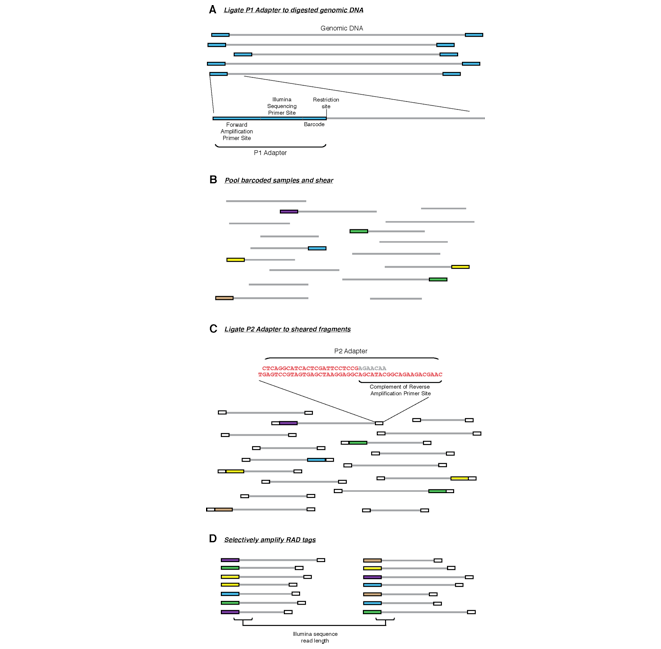
\includegraphics{02_Molecular/./images/seq_radmark_fig1.png}

}

\caption{IMAGE TO BE INCLUDED LATER}

\end{figure}

Fig. 1. RAD tag library generation. (A) Genomic DNA is digested with a
restriction enzyme and a barcoded P1 adapter is ligated to the
fragments. The P1 adapter contains a forward amplification primer site,
an Illumina sequencing primer site, and a barcode (colored boxes
represent P1 adapters with different barcodes). (B) Adapter-ligated
fragments are combined (if multiplexing), sheared and (C) ligated to a
second adapter (P2, white boxes). The P2 adapter is a divergent ``Y''
adapter, containing the reverse complement of the P2 reverse
amplification primer site, preventing amplification of genomic fragments
lacking a P1 adapter. (D) RAD tags, which have a P1 adapter, are
selectively and robustly enriched by PCR amplification. (Reproduced from
ref. 12 with permission from PLoS). (ref. 9 with permission from
Elsevier Science). {[}Baird et al., 2008{]}

\hypertarget{dna-extraction-and-rnase-a-treatment-1}{%
\subsection{DNA extraction and RNase A
treatment}\label{dna-extraction-and-rnase-a-treatment-1}}

\begin{itemize}
\tightlist
\item
  We recommend extracting genomic DNA samples using the DNeasy Blood \&
  Tissue Kit (Qiagen) or a similar product that produces very pure, high
  molecular weight, RNA-free DNA.
\item
  High-quality DNA is required for optimal restriction endonuclease
  digestion and is of utmost importance for the overall success of the
  protocol.
\item
  Follow the manufacturers instructions for extraction from your tissue
  type.
\item
  Be sure to treat samples with RNase A following manufacturer's
  instructions to remove residual RNA.
\item
  Quantify the DNA using a fluorimeter to get the most accurate
  concentration readings (see Note 3).
\item
  The optimal concentration after elution is 25 ng/μl or greater.
\end{itemize}

\hypertarget{restriction-endonuclease-digestion-1}{%
\subsection{Restriction endonuclease
digestion}\label{restriction-endonuclease-digestion-1}}

\begin{enumerate}
\def\labelenumi{\arabic{enumi}.}
\item
  Digest 1μg genomic DNA for each individual sample, or a mix of pooled
  individuals sharing a common phenotype, with appropriate restriction
  enzyme in a 50 μl reaction volume, following the manufacturers
  instructions.
\item
  In a microcentrifuge tube combine: 5.0 μl 10X NEB Buffer 2, 0.5 μl
  EcoRI, DNA and H2O to 50.0 μl.
\item
  Use NEB Buffer 4 with High Fidelity enzymes, e.g., SbfI-HF. Set up
  larger reaction if necessary because of dilute DNA -- concentrate with
  a Zymo column before proceeding to ligation or adjust ligation
  volumes. 1.5 hours SbfI incubation. Heat inactivate 65°C for 25
  min.{]}
\item
  Heat-inactivate the restriction enzyme following manufacturer's
  instructions. Allow reaction to cool slowly to ambient temperature
  (30-60 min). If the enzyme cannot be heat-inactivated, purify with a
  QIAquick or Zymo column following manufacturer's instructions prior to
  ligation.
\end{enumerate}

\hypertarget{p1-adapter-ligation-1}{%
\subsection{P1 Adapter ligation}\label{p1-adapter-ligation-1}}

\begin{enumerate}
\def\labelenumi{\arabic{enumi}.}
\tightlist
\item
  This step in the protocol ligates barcoded, restriction-site overhang
  specific P1 adapters onto complementary compatible ends on the genomic
  DNA created in the previous step (see Note 5). In Baird et al., 2008
  (12) 60 different barcoded P1 adapters were used to make EcoRI RAD tag
  libraries for 96 F2 individuals (see Note 7).
\item
  To each inactivated digest, add: 1.0 μl 10X NEB Buffer 2, 5.0 μl
  Barcoded P1 Adapter (100 nM), 0.6 μl rATP (100 mM), 0.5 μl
  concentrated T4 DNA Ligase (2,000,000 U/ml), 2.9 μl H2O; 60.0 μl total
  volume. Be sure to add P1 adapters to the reaction before the Ligase
  to avoid re-ligation of the genomic DNA. Incubate reaction at room
  temperature for at least 30 min. or 1 hr at RT then overnight at 4C
  (ligase will still be active, but slow at 4C -- the longer incubation
  time assumes that there is no exonuclease activity in the ligase).
\item
  NEB Buffer 2 is used in the ligation reactions in this protocol
  instead of ligase buffer because the salt it contains (50 mM NaCl)
  ensures the double-stranded adapters remain annealed during the
  reactions (see Note 4). T4 DNA Ligase is active in all 4 NEB Buffers
  if supplemented with 1mM rATP, but doesn't work at maximum efficiency
  in NEB 3. If the restriction buffer used for digestion does not
  contain at least 50 mM potassium or sodium ions, or if the
  endonuclease cannot be heat-inactivated and the reaction must be
  purified in a column prior to P1 ligation, add 6.0 μl NEB Buffer 2.
\item
  Reduce the amount of P1 used in the ligation reaction if starting with
  less than 1μg genomic DNA or if cutting with an enzyme that cuts less
  frequently than EcoRI (e.g., use 2.5 µl adapter if using SbfI in
  stickleback). It is critical to optimize the amount of P1 adapter
  added when a given restriction enzyme is used for the first time in an
  organism (see Note 6).
\item
  Heat-inactivate T4 DNA Ligase for 20 (25) min at 65° C. Allow reaction
  to cool slowly to ambient temperature (30 min).
\end{enumerate}

\hypertarget{sample-multiplexing}{%
\subsection{Sample multiplexing}\label{sample-multiplexing}}

\begin{enumerate}
\def\labelenumi{\arabic{enumi}.}
\tightlist
\item
  This step allows multiple individually barcoded samples to be combined
  and processed as one to cut down on cost, work time, and differences
  in amplification efficiency that may arise between different library
  preparations when processing many at once.
\item
  Combine barcoded samples at desired ratio. Use a 100-300 μl aliquot
  containing 1-2 μg DNA total to complete the protocol and freeze the
  rest at -20° C. In Baird et al., 2008 (12) F0 parent samples, as well
  as the F2 pools used for bulk-segregant analysis, were combined at
  equal volumes to create one library (see Fig. 2, lanes 2, 3 \& 5).
  EcoRI libraries containing barcoded samples from F2 individuals
  sharing a given lateral plate phenotype were pooled and processed as
  separate libraries after P1 ligation (see Note 7).
\end{enumerate}

\hypertarget{dna-shearing-1}{%
\subsection{DNA shearing}\label{dna-shearing-1}}

\begin{enumerate}
\def\labelenumi{\arabic{enumi}.}
\tightlist
\item
  Shear DNA samples to an average size of 500 bp to create a library of
  P1/restriction-site-ligated molecules with random variable ends for
  amplification. This step requires some optimization for different DNA
  concentrations and each time a different restriction endonuclease is
  used. The following protocol has been optimized to shear Stickleback
  DNA digested with either EcoRI or SbfI using the Bioruptor and is a
  good starting point for any study. The goal is to create sheared
  product that is predominantly smaller than 1 kb in size (see Fig. 2).
\item
  Dilute ligation reaction to 100 μl in water (or take 100-300 μl
  aliquot from multiplexed samples) and shear in Bioruptor 10 times for
  30 sec on high following manufacturer's instructions. Make sure the
  tank water in the Bioruptor is cold (4 C) before starting -- bail out
  and replace with chilled water if necessary. All other positions in
  the Bioruptor holder that are not filled by your sample/s should be
  filled with balance tubes containing 100 microliters of water.
\item
  Clean up sheared DNA sample(s) using a MinElute or Zymo column
  following manufacturer's instructions. This purification is performed
  in order to remove the ligase and restriction enzymes, and to
  concentrate the DNA so that the entire sample can be loaded in a
  single lane on an agarose gel. Elute in 20 μl EB.
\end{enumerate}

\hypertarget{size-selectionagarose-gel-extraction-1}{%
\subsection{Size selection/agarose gel
extraction}\label{size-selectionagarose-gel-extraction-1}}

\begin{enumerate}
\def\labelenumi{\arabic{enumi}.}
\tightlist
\item
  This step in the protocol removes free un-ligated or concatamerized P1
  adapters and restricts the size range of tags to that which can be
  sequenced efficiently on an Illumina Genome Analyzer flow cell. Run
  the entire sheared sample in 1X Orange Loading Dye on a 1.25\%
  agarose, 0.5X TBE gel for 45 min at 100 V, next to 2.0 μl GeneRuler
  100 bp DNA Ladder Plus for size reference (see Fig. 2, Note 8).
\item
  Being careful to exclude any free P1 adapters and P1 dimers running at
  \textasciitilde130 bp and below, use a fresh razor blade to cut a
  slice of the gel spanning 300-500 bp. Extract DNA using MinElute Gel
  Purification Kit following manufacturer's instructions with the
  following modification: to improve representation of A + T-rich
  sequences, melt agarose gel slices in the supplied buffer at room
  temperature (18-22°C) with agitation for 30 min (14). Elute in 20 μl
  EB into eppendorf tube containing 2.5 μl 10X Blunting Buffer from
  Quick Blunting Kit used in the following step. {[}Use MinElute columns
  and not Qiaquick columns, which require a larger elution volume{]}
\end{enumerate}

\hypertarget{perform-end-repair-1}{%
\subsection{Perform end repair}\label{perform-end-repair-1}}

\begin{enumerate}
\def\labelenumi{\arabic{enumi}.}
\tightlist
\item
  The Quick Blunting Kit protocol converts 5´ or 3´ overhangs, created
  by shearing, into phosphorylated blunt ends using T4 DNA Polymerase
  and T4 Polynucleotide Kinase.
\item
  To the eluate from the previous step, add: 2.5 μl dNTP mix (1mM), 1.0
  μl Blunt Enzyme Mix. Incubate at RT for 30 min.
\item
  Purify with QIAquick or Zymo column. Elute in 43 μl EB (42 µl if using
  Zymo column) into eppendorf tube containing 5.0 μl 10X NEB Buffer 2.
\end{enumerate}

\hypertarget{da-overhang-addition-1}{%
\subsection{3´-dA overhang addition}\label{da-overhang-addition-1}}

\begin{enumerate}
\def\labelenumi{\arabic{enumi}.}
\tightlist
\item
  This step in the protocol adds an `A' base to the 3´ ends of the blunt
  phosphorylated DNA gfragments, using the polymerase activity of Klenow
  Fragment (3´ to 5´ exo-). This prepares the DNA fragments for ligation
  to the P2 adapter, which possesses a single `T' base overhang at the
  3´ end of its bottom strand.
\item
  To the eluate from the previous step, add: 1.0 μl dATP (10mM), 3.0 μl
  Klenow (exo-). Incubate at 37º C for 30 min. Allow reaction to cool
  slowly to ambient temperature (15 min).
\item
  Purify with QIAquick or Zymo column. Elute in 45 μl EB (44 µl if using
  Zymo) into eppendorf tube containing 5.0 μl 10X NEB Buffer 2
\end{enumerate}

\hypertarget{p2-adapter-ligation-1}{%
\subsection{P2 Adapter ligation}\label{p2-adapter-ligation-1}}

\begin{enumerate}
\def\labelenumi{\arabic{enumi}.}
\tightlist
\item
  This step in the protocol ligates the P2 adapter, a ``Y'' adapter with
  divergent ends that contains a 3´ dT overhang, onto the ends of blunt
  DNA fragments with 3´ dA overhangs.
\item
  To the eluate from previous step, add: 1.0 μl P2 Adapter (10 μM), 0.5
  μl rATP (100 mM), 0.5 μl concentrated T4 DNA Ligase. Incubate reaction
  at room temperature for 30 min. to 1 hour at RT then overnight (the
  longer incubation time assumes that there is no exonuclease activity
  in the ligase).
\item
  Purify with QIAquick or Zymo column. Elute in 52 μl EB (or 2 x 10 µl,
  for more concentrated sample).
\end{enumerate}

\hypertarget{rad-tag-amplificationenrichment-1}{%
\subsection{RAD tag
Amplification/Enrichment}\label{rad-tag-amplificationenrichment-1}}

\begin{enumerate}
\def\labelenumi{\arabic{enumi}.}
\tightlist
\item
  In this step you will perform high-fidelity PCR amplification on P1
  and P2 adapter-ligated DNA fragments, enriching for RAD tags that
  contain both a P1 and P2 and preparing them to be hybridized to an
  Illumina Genome Analyzer flow cell (see Fig. 1).
\item
  Perform a test amplification to determine library quality. In
  thin-walled PCR tube, combine: 10.5 μl H2O, 12.5 μl Phusion
  High-Fidelity Master Mix, 1.0 μl Solexa primer mix (10 μM), 1.0 μl RAD
  library template (eluate from last step). If using concentrated
  Phusion enzyme (i.e., not Master Mix), instead combine: 17.25 µl H2O,
  5 µl Phusion HF buffer, 0.5 µl 10 mM dNTPs, 1 µl primer mix, 1 µl
  template, 0.25 µl Phusion DNA polymerase. Perform 18 cycles of
  amplification in thermal cycler: 30 sec 98° C, 18X (or 14X) {[}10 sec
  98° C, 30 sec 65° C, 30 sec 72° C{]}, 5 min 72° C, hold 4° C. Run 5.0
  μl PCR product in 1X Orange Loading Dye out on 1.0\% agarose gel next
  to 1.0 μl RAD library template and 2.0 μl GeneRuler 100 bp DNA Ladder
  Plus (Fig. 3), (or clean whole reaction with Zymo column, elute in 2 x
  10 µl EB and run all on gel).
\item
  If the amplified product is at least twice as bright as the template,
  perform a larger volume amplification (typically 50-100 μl) but with
  fewer cycles (10-14, usually 12, to minimize bias), to create enough
  to retrieve a large amount of the RAD tag library from the final gel
  extraction in the protocol. If amplification looks poor, use more
  library template in a second test PCR reaction (see Note 9). Fig. 3
  shows three libraries that amplified well, which is apparent when
  comparing the amplified product to the amount of template loaded in
  the lane to the right of each sample. Template should be dim, yet
  visible on the gel. Purify large volume reaction with a MinElute or
  Zymo column. Elute in 20 μl EB (or 2 x 10 µl)
\item
  This purification step is performed to eliminate any contaminant bands
  that may appear due to an improper ratio of P1 adapter to
  restriction-site compatible ends (see Note 6). Load entire sample in
  1X Orange Loading Dye on a 1.25\% agarose, 0.5X TBE gel and run for 45
  min at 100 V, next to 2.0 μl GeneRuler 100 bp DNA Ladder Plus for size
  reference (Fig. 4). Being careful to exclude any free adapters or P1
  dimer contaminants running at \textasciitilde130 bp and below, use a
  fresh razor blade to cut a slice of the gel spanning 300-500 bp (or
  rather, 385-585 bp, which accounts for extra length of
  post-amplification adapters). Extract DNA using MinElute Gel
  Purification Kit following manufacturer's instructions. Melt agarose
  gel slices in the supplied buffer at room temperature. Elute in 20 μl
  EB.
\item
  Quantify the DNA using a fluorimeter to get the most accurate
  concentration readings. Concentrations will range from 1-20 ng/μl.
  Determine the molar concentration of the library by examining the gel
  image and estimating the median size of the library smear, which
  should be around 400 bp. Multiply this size by 650 (the molecular mass
  of a base-pair) to get the molecular weight of the library. Use this
  number to calculate the molar concentration of the library (see Note
  10)
\item
  Validate library by cloning 1.0 μl of the gel purified library into a
  blunt-end compatible sequencing vector. Sequence individual clones by
  conventional Sanger sequencing. Verify that the insert sequences are
  from the genomic source DNA.
\item
  Sequence libraries on Illumina Genome Analyzer following
  manufacturer's instructions.
\end{enumerate}

\hypertarget{sec-molecular-T_overhang}{%
\chapter{T-overhang addition}\label{sec-molecular-T_overhang}}

\hypertarget{introduction-24}{%
\section{Introduction}\label{introduction-24}}

\begin{itemize}
\tightlist
\item
  \textbf{Purpose}: This protocol will add a t-overhang to PCR or other
  genomic DNA fragments for the purposes of cloning or Illumina
  sequencing.
\item
  \textbf{Procedure Type}: Molecular
\item
  \textbf{Species}: N/A
\item
  \textbf{Author}: xxx
\item
  \textbf{Date Created}: xxx
\end{itemize}

\begin{tcolorbox}[enhanced jigsaw, rightrule=.15mm, title=\textcolor{quarto-callout-warning-color}{\faExclamationTriangle}\hspace{0.5em}{NOTES}, titlerule=0mm, opacitybacktitle=0.6, toprule=.15mm, bottomrule=.15mm, opacityback=0, left=2mm, colframe=quarto-callout-warning-color-frame, breakable, coltitle=black, colback=white, colbacktitle=quarto-callout-warning-color!10!white, bottomtitle=1mm, leftrule=.75mm, toptitle=1mm, arc=.35mm]

xxxx

\end{tcolorbox}

\hypertarget{materials-24}{%
\section{Materials:}\label{materials-24}}

\begin{itemize}
\tightlist
\item
  2.5 µl 10 X buffer
\item
  2.5 µl 1 mM dNTP mix
\item
  1 µl enzyme
\item
  5 µl 10x Klenow Exo- buffer (Epicentre)
\item
  1 µl dATP 10 mM
\item
  3 µl 5 u/µl Klenow Exo- (Epicentre)
\item
  5 µl 10x NEB buffer 2
\item
  0.5 µl rATP 100 mM
\item
  x µl of 10 µm* T-overhang PE adapter
\item
  x µl water to 49.5 µl total
\item
  0.5 µl T4 DNA ligase (10 u/µl, Epicentre)
\item
  2.5 \% agarose gel
\item
  QG
\item
  Qiagen gel extraction kit
\item
  MinElute columns
\item
  Zymo DNA column
\end{itemize}

\hypertarget{procedure-23}{%
\section{Procedure}\label{procedure-23}}

\hypertarget{shearing}{%
\subsection{Shearing:}\label{shearing}}

\begin{itemize}
\tightlist
\item
  Up to 1 µg\textsuperscript{†} DNA in 100 microliters in EB (in 0.6 ml
  tubes, Axygen) -- fill all other positions in Bioruptor holder with
  tubes containing 100 µl water. Before beginning, make sure Bioruptor
  tank water is 4°C or less -- bail out and replace with chilled water
  if necessary and add a little crushed ice to the tank.
\item
  Set the controls to shear 30 sec.~on, 30 sec.~off for 15 cycles
\item
  After cycling, replace tank water with cold water and a little ice
\item
  Repeat shearing (i.e., another 15 cycles)
\item
  Zymo column concentrate -- elute 2 times with 10.5 µl EB.
\end{itemize}

\begin{tcolorbox}[enhanced jigsaw, rightrule=.15mm, title=\textcolor{quarto-callout-warning-color}{\faExclamationTriangle}\hspace{0.5em}{NOTES}, titlerule=0mm, opacitybacktitle=0.6, toprule=.15mm, bottomrule=.15mm, opacityback=0, left=2mm, colframe=quarto-callout-warning-color-frame, breakable, coltitle=black, colback=white, colbacktitle=quarto-callout-warning-color!10!white, bottomtitle=1mm, leftrule=.75mm, toptitle=1mm, arc=.35mm]

If you start with greater than 1 µg (up to 2 µg), you will either have
to scale up the volume of the ligation, decrease the amount of EB used
in the elution after addition of A overhangs, or make a batch of
annealed adapter that is greater than 10 µM in order to maintain a 10:1
ratio of adapter to fragmented DNA in the ligation reaction.

\end{tcolorbox}

\hypertarget{end-repair}{%
\subsection{End repair:}\label{end-repair}}

To eluate, add NEB Quick Blunting kit reagents:

\begin{itemize}
\tightlist
\item
  2.5 µl 10 X buffer
\item
  2.5 µl 1 mM dNTP mix
\item
  1 µl enzyme
\end{itemize}

Then:

\begin{itemize}
\tightlist
\item
  30 min at room temperature
\item
  Clean with Zymo column, elute 2 times with 21 µl EB.
\end{itemize}

\hypertarget{addition-of-a-overhangs}{%
\subsection{Addition of A overhangs:}\label{addition-of-a-overhangs}}

To eluate, add:

\begin{itemize}
\tightlist
\item
  5 µl 10x Klenow Exo- buffer (Epicentre)
\item
  1 µl dATP 10 mM
\item
  3 µl 5 u/µl Klenow Exo- (Epicentre)
\end{itemize}

Then:

\begin{itemize}
\tightlist
\item
  30 min at 37°C
\item
  Clean with Zymo column, elute 2 times with 20 µl EB
\end{itemize}

\hypertarget{ligation}{%
\subsection{Ligation:}\label{ligation}}

To eluate, add:

\begin{itemize}
\tightlist
\item
  5 µl 10x NEB buffer 2
\item
  0.5 µl rATP 100 mM
\item
  x µl of 10 µm* T-overhang PE adapter
\item
  x µl water to 49.5 µl total
\item
  0.5 µl T4 DNA ligase (10 u/µl, Epicentre)
\item
  1 hour to overnight at RT
\end{itemize}

\begin{tcolorbox}[enhanced jigsaw, rightrule=.15mm, title=\textcolor{quarto-callout-warning-color}{\faExclamationTriangle}\hspace{0.5em}{NOTES}, titlerule=0mm, opacitybacktitle=0.6, toprule=.15mm, bottomrule=.15mm, opacityback=0, left=2mm, colframe=quarto-callout-warning-color-frame, breakable, coltitle=black, colback=white, colbacktitle=quarto-callout-warning-color!10!white, bottomtitle=1mm, leftrule=.75mm, toptitle=1mm, arc=.35mm]

You should scale the adapter concentration to the amount of DNA used,
maintaining an approximate 10:1 molar ratio of adapter to fragments.
Assuming the average size of sheared fragments is 350 bp, 228 ng should
equal about 1 pmol. Starting with 1 µg, then, we'd have about 4.4 pmol.
10 times that would be 44 pmol of adapter or 4.4 µl of 10 µM adapter. In
reality, there is probably some loss of a percentage of cDNA during
cleanups, incomplete efficiency of blunting and A-overhang addition and
less than ideal shearing, all driving down the molarity of ligatable
fragments, so you can probably get away with adding less adapter than
calculated from the ideal. If you see a faint band of unincorporated
adapter in your size fractionation gel, that is probably a good
indication that you have saturated but not grossly exceeded the amount
of adapter needed.

\end{tcolorbox}

\hypertarget{alternatives}{%
\section{Alternatives}\label{alternatives}}

\hypertarget{alternative-a.}{%
\subsection{Alternative A.}\label{alternative-a.}}

\begin{itemize}
\tightlist
\item
  Zymo column purify, elute 2 times with 6 µl and proceed to
  amplification before size fractionation.
\item
  Only do this if there is a vanishingly small amount of material. It is
  probably better to size-fractionate before amplification.
\end{itemize}

\hypertarget{alternative-b.}{%
\subsection{Alternative B.}\label{alternative-b.}}

\begin{itemize}
\tightlist
\item
  Zymo column purify, elute 2 times with 10 µl and size fractionate (see
  below)
\item
  Size fractionation: 2.5 \% agarose gel Cut 200 -- 500, carefully
  avoiding any unincorporated adaptor.
\item
  If desired, also cut 500-700 bp fraction.
\item
  These two fractions should constitute most of the sheared cDNA.
\item
  The smaller size range may be less biased against short transcripts.
  Recover DNA with Qiagen gel extraction kit and MinElute columns.
\item
  Dissolve gel at room temperature in 6 volumes QG. Follow manufacturer
  instructions, being sure to let wash buffer stand on column for at
  least 5 min. before spinning through.
\item
  Elute 2 times with 10 µl EB. Check concentration on Qubit fluorometer
  using Quant-It HS (high sensitivity) kit.
\end{itemize}

\hypertarget{sec-molecular-TopoClone}{%
\chapter{Topo Cloning}\label{sec-molecular-TopoClone}}

\hypertarget{introduction-25}{%
\section{Introduction}\label{introduction-25}}

\begin{itemize}
\tightlist
\item
  \textbf{Purpose}: This procedure describes how to TOPO Clone with pCR4
  Vector.
\item
  \textbf{Procedure Type}: xxx
\item
  \textbf{Species}: N/A
\item
  \textbf{Author}: xxx
\item
  \textbf{Date Created}: xxx
\end{itemize}

\begin{tcolorbox}[enhanced jigsaw, rightrule=.15mm, title=\textcolor{quarto-callout-warning-color}{\faExclamationTriangle}\hspace{0.5em}{NOTES}, titlerule=0mm, opacitybacktitle=0.6, toprule=.15mm, bottomrule=.15mm, opacityback=0, left=2mm, colframe=quarto-callout-warning-color-frame, breakable, coltitle=black, colback=white, colbacktitle=quarto-callout-warning-color!10!white, bottomtitle=1mm, leftrule=.75mm, toptitle=1mm, arc=.35mm]

xxxx

\end{tcolorbox}

\hypertarget{materials-25}{%
\section{Materials:}\label{materials-25}}

\begin{itemize}
\tightlist
\item
  1 μl of salt solution
\item
  0.5 μl of vector
\item
  20 μl of TOP10 chemically competent cells
\item
  ice
\item
  400 μl of room temp SOC
\item
  bacterial plates
\item
  50 μl LB-Amp in round bottom plates
\item
  10.0 μl Lab PCR mix
\item
  0.25 μl T3/T7 Primer Pair
\item
  0.1 μl Taq
\item
  50 μl LB-Amp
\item
  14\% Glycerol
\end{itemize}

\hypertarget{procedure-24}{%
\section{Procedure:}\label{procedure-24}}

\hypertarget{topo-clone-with-pcr4-vector}{%
\subsection{TOPO Clone With pCR4
Vector}\label{topo-clone-with-pcr4-vector}}

\begin{enumerate}
\def\labelenumi{\arabic{enumi}.}
\tightlist
\item
  Cut PCR bands from gels, freeze
\item
  Vortex band tubes, then spin at 14000RPM for 10 min
\item
  place at room temperature for 20 min
\item
  add 20 μl of TOP10 chemically competent cells
\item
  back on ice for 30 min
\item
  heat shock at 42°C for 30 sec
\item
  add 400 μl of room temp SOC, place at 37°C for one hour
\item
  spread onto plates
\item
  incubate overnight at 37°C
\end{enumerate}

\hypertarget{pcr-screen-for-inserts}{%
\subsection{PCR screen for Inserts}\label{pcr-screen-for-inserts}}

\begin{enumerate}
\def\labelenumi{\arabic{enumi}.}
\tightlist
\item
  Pick colonies from each plate with toothpick
\item
  Into 50 μl LB-Amp in round bottom plates, 37°C for one hour
\item
  Use 2 μl as template for PCR reaction, put plate back at 37°C
\end{enumerate}

\begin{longtable}[]{@{}lccrl@{}}
\toprule\noalign{}
\endhead
\bottomrule\noalign{}
\endlastfoot
Step 1 & - & 94°C - & 5 min & \\
Step 2 & - & 94°C - & 45 sec & \\
Step 3 & - & 56°C - & 45 sec & \\
Step 4 & - & 72°C - & 1 min & 37X for steps 2-4 \\
Step 5 & - & 72°C - & 5 min & \\
Step 6 & - & 12°C - & indef & \\
\end{longtable}

\hypertarget{overnight}{%
\subsection{Overnight:}\label{overnight}}

\begin{itemize}
\tightlist
\item
  Use 2 μl to inoculate 5 ml of LB-Amp, shake at 37°C overnight
\item
  Qiagen miniprep next day, ready to sequence
\end{itemize}

\hypertarget{storage-of-clones}{%
\subsection{Storage of Clones:}\label{storage-of-clones}}

\begin{itemize}
\tightlist
\item
  Grow clone plates overnight at 37°C
\item
  Next morning, add 50 μl LB-Amp, 14\% Glycerol to each well (7\% final)
\item
  Freeze for long term storage
\end{itemize}

\hypertarget{sec-molecular-TopoClone_PCR4}{%
\chapter{TopoClone with PCR4
Vector}\label{sec-molecular-TopoClone_PCR4}}

\hypertarget{introduction-26}{%
\section{Introduction}\label{introduction-26}}

\begin{itemize}
\item
  \textbf{Purpose}: This procedure describes how to TopoClone with PCR4
  Vector.
\item
  \textbf{Procedure Type}: Molecular
\item
  \textbf{Author}: Susie Bassham
\item
  \textbf{Date Created}: xxx
\end{itemize}

\hypertarget{materials-26}{%
\section{Materials}\label{materials-26}}

\begin{itemize}
\item
  ice
\item
  bacterial plates
\item
  50 μl LB-Amp in round bottom plates
\end{itemize}

\hypertarget{solutions-21}{%
\section{Solutions}\label{solutions-21}}

\begin{itemize}
\tightlist
\item
  0.5 μl of salt solution
\item
  0.5 μl of vector
\item
  20 μl of TOP10 chemically competent cells
\item
  400 μl of room temp SOC
\item
  10.0 μl Lab PCR mix
\item
  0.25 μl T3/T7 Primer Pair
\item
  0.1 μl Taq
\item
  50 μl LB-Amp
\item
  14\% Glycerol
\end{itemize}

\hypertarget{procedure-25}{%
\section{Procedure}\label{procedure-25}}

\begin{enumerate}
\def\labelenumi{\arabic{enumi}.}
\item
  \textbf{TopoClone with PCR4 Vector}

  \begin{enumerate}
  \def\labelenumii{\arabic{enumii}.}
  \tightlist
  \item
    Cut PCR bands from gels, freeze
  \item
    Vortex band tubes, then spin at 14000RPM for 10min
  \end{enumerate}

  \begin{tcolorbox}[enhanced jigsaw, rightrule=.15mm, title=\textcolor{quarto-callout-important-color}{\faExclamation}\hspace{0.5em}{NOTE}, titlerule=0mm, opacitybacktitle=0.6, toprule=.15mm, bottomrule=.15mm, opacityback=0, left=2mm, colframe=quarto-callout-important-color-frame, breakable, coltitle=black, colback=white, colbacktitle=quarto-callout-important-color!10!white, bottomtitle=1mm, leftrule=.75mm, toptitle=1mm, arc=.35mm]

  electrophoresis should be carried out in TAE buffer not TBE because
  the borate in TBE will interfere with ligation

  \end{tcolorbox}

  \begin{tcolorbox}[enhanced jigsaw, rightrule=.15mm, title=\textcolor{quarto-callout-important-color}{\faExclamation}\hspace{0.5em}{NOTE}, titlerule=0mm, opacitybacktitle=0.6, toprule=.15mm, bottomrule=.15mm, opacityback=0, left=2mm, colframe=quarto-callout-important-color-frame, breakable, coltitle=black, colback=white, colbacktitle=quarto-callout-important-color!10!white, bottomtitle=1mm, leftrule=.75mm, toptitle=1mm, arc=.35mm]

  if the PCR was carried out with an error correcting polymerase like
  Phusion, you will need to clean the reaction with beads or column and
  A-tail the products with dATP and wild-type Taq or with Klenow exo-
  before TA cloning.

  \end{tcolorbox}

  \begin{enumerate}
  \def\labelenumii{\arabic{enumii}.}
  \setcounter{enumii}{2}
  \tightlist
  \item
    1X cloning reaction

    \begin{enumerate}
    \def\labelenumiii{\arabic{enumiii}.}
    \tightlist
    \item
      2 μl of supernatant from each tube
    \item
      0.5 μl of salt solution
    \item
      0.5 μl of vector
    \item
      place at room temperature for 20min
    \item
      add 20 μl of TOP10 chemically competent cells back on ice for 30
      min 6 heat shock at42C for 30 sec
    \item
      add 400 μl of room temp SOC, place at 37C for one hour
    \item
      spread onto plates
    \item
      incubate overnight at 37C
    \end{enumerate}
  \end{enumerate}
\item
  \textbf{PCR Screen for Inserts}

  \begin{enumerate}
  \def\labelenumii{\arabic{enumii}.}
  \tightlist
  \item
    Pick colonies from each plate with toothpick
  \item
    Into 50 μl LB-Amp in round bottom plates, 37C for one hour
  \item
    Use 2 μl as template for PCR reaction, put plate back at 37C
  \end{enumerate}

  1X PCR Reaction - 10.0 μl Lab PCR mix - 0.25 μl T3/T7 Primer Pair -
  0.1 μl Taq

  \begin{longtable}[]{@{}lllll@{}}
  \toprule\noalign{}
  94C & - & 5 min & - & - \\
  \midrule\noalign{}
  \endhead
  \bottomrule\noalign{}
  \endlastfoot
  - & 94C & - & 45 sec & \\
  - & 56C & - & 45 sec & 37X \\
  - & 72C & - & 1 min & \\
  72C & - & 5 min & - & \\
  12C & - & indefinite & - & \\
  \end{longtable}
\item
  \textbf{Overnight}

  \begin{enumerate}
  \def\labelenumii{\arabic{enumii}.}
  \tightlist
  \item
    Use 2 μl to inoculate 5ml of LB-Amp, shake at 37C overnight
  \item
    Qiagen miniprep next day, ready to sequence.
  \end{enumerate}
\item
  \textbf{Storage of Clones}

  \begin{enumerate}
  \def\labelenumii{\arabic{enumii}.}
  \tightlist
  \item
    Grow clone plates overnight at 37C
  \item
    Next morning, add 50 μl LB-Amp, 14\% Glycerol to each well (7\%
    final)
  \item
    Freeze for long term storage
  \end{enumerate}
\end{enumerate}

\hypertarget{associated-papers-15}{%
\section{Associated Papers}\label{associated-papers-15}}

\begin{itemize}
\tightlist
\item
  xxx
\item
  xxx
\item
  xxx
\end{itemize}

\part{Microbiology}

This ection of the book contains protocols that involve the use of
microbes, mostly in the context of host-microbe interactions, but also
standard protocols for cloning of nucleic acides using microbes.

\hypertarget{sec-microbiology}{%
\chapter{Placeholder\_Microbiology}\label{sec-microbiology}}

\hypertarget{xxx}{%
\section{xxx}\label{xxx}}

xxxx

\hypertarget{xxx-1}{%
\subsection{xxx}\label{xxx-1}}

xxxxx

\part{Vertebrate Husbandry}

This section of the manual contains protocols for the safe and ethical
husbandry and use of vertebrate animals, particular the fish models
stickleback, zebrafish and syngnathids.

\hypertarget{sec-husbandry-autoclaving}{%
\chapter{Autoclaving Fish Room}\label{sec-husbandry-autoclaving}}

\hypertarget{introduction-27}{%
\section{Introduction}\label{introduction-27}}

\begin{itemize}
\tightlist
\item
  \textbf{Purpose}: For sanitizing nets and scrub pads that have been
  used in the fish room.
\item
  \textbf{Procedure Type}: xxx
\item
  \textbf{Species}:

  \begin{itemize}
  \tightlist
  \item
    Threespine stickleback, (\emph{Gasterosteus aculeatus})
  \item
    Bay pipefish, (\emph{Syngnathus leptorhyncus})
  \item
    Gulf pipefish (\emph{Syngnathus scovelli})
  \item
    Zebrafish, (\emph{Danio rerio})
  \end{itemize}
\item
  \textbf{Author}: xxx
\item
  \textbf{Date Created}: xxx
\end{itemize}

\begin{tcolorbox}[enhanced jigsaw, rightrule=.15mm, title=\textcolor{quarto-callout-warning-color}{\faExclamationTriangle}\hspace{0.5em}{NOTES}, titlerule=0mm, opacitybacktitle=0.6, toprule=.15mm, bottomrule=.15mm, opacityback=0, left=2mm, colframe=quarto-callout-warning-color-frame, breakable, coltitle=black, colback=white, colbacktitle=quarto-callout-warning-color!10!white, bottomtitle=1mm, leftrule=.75mm, toptitle=1mm, arc=.35mm]

xxxx

\end{tcolorbox}

\hypertarget{materials-27}{%
\section{Materials}\label{materials-27}}

\begin{itemize}
\tightlist
\item
  xx
\item
  xx
\item
  xx
\end{itemize}

\hypertarget{procedure-26}{%
\section{Procedure}\label{procedure-26}}

\begin{enumerate}
\def\labelenumi{\arabic{enumi}.}
\tightlist
\item
  Place dirty nets and scrub pads in autoclave wire bin
\item
  Put bin into autoclave, and close the door (close door by pushing main
  door against hinge on left of door, then push door shut and seal by
  turning handle clockwise to just tight, DO NOT OVER TIGHTEN).
\item
  Change menu to B using keypad
\item
  Hit \#1 twice, this will start the autoclave.
\item
  Sign sheet on outside of entrance door
\item
  Wait 45 minutes and remove nets
\item
  Put nets in clean nets tub.
\item
  Initial Check list on outside of door.~~~\textbf{Gravity~~~45 min~~~OK
  to Remove}
\end{enumerate}

\hypertarget{sec-husbandry-20gal_tank_cleaning}{%
\chapter{Tank Cleaning 20G}\label{sec-husbandry-20gal_tank_cleaning}}

\hypertarget{introduction-28}{%
\section{Introduction}\label{introduction-28}}

\begin{itemize}
\tightlist
\item
  \textbf{Purpose}: This procedure describes how to clean 20 gallon
  glass tanks.
\item
  \textbf{Procedure Type}: Husbandry
\item
  \textbf{Species}:

  \begin{itemize}
  \tightlist
  \item
    Threespine stickleback, (\emph{Gasterosteus aculeatus})
  \item
    Gulf pipefish (\emph{Syngnathus scovelli})
  \end{itemize}
\item
  \textbf{Author}: Mark Currey
\item
  \textbf{Date Created}: April 8, 2008; revised December 6, 2018 by M.
  Currey
\end{itemize}

\begin{tcolorbox}[enhanced jigsaw, rightrule=.15mm, title=\textcolor{quarto-callout-important-color}{\faExclamation}\hspace{0.5em}{This is important}, titlerule=0mm, opacitybacktitle=0.6, toprule=.15mm, bottomrule=.15mm, opacityback=0, left=2mm, colframe=quarto-callout-important-color-frame, breakable, coltitle=black, colback=white, colbacktitle=quarto-callout-important-color!10!white, bottomtitle=1mm, leftrule=.75mm, toptitle=1mm, arc=.35mm]

Tank cleaning is to be done \textbf{ONLY Monday - Friday}.

\end{tcolorbox}

\hypertarget{materials-28}{%
\section{Materials}\label{materials-28}}

\begin{itemize}
\tightlist
\item
  Scrub pad or sponge
\item
  Cart
\item
  Old clothes (this can be messy)
\item
  Personal protection equipment (Splash proof glasses or face shield)
\item
  Gloves
\item
  Sink
\end{itemize}

\hypertarget{solutions-22}{%
\section{Solutions}\label{solutions-22}}

\begin{itemize}
\tightlist
\item
  \textbf{Bleach solution}: Make a 10\% bleach solution in a used 1
  gallon bleach bottle. To do so: Add 2.7 L of water. Add 0.3 L of
  bleach and gently stir. Dispense into appropriately labeled squirt
  bottle for use.
\item
  \textbf{Sodium thiosulfate}: Make a 5\% solution of sodium thiosulfate
  in the carboy located on counter above the fridge. To do so: Add 500 g
  of sodium thiosulfate. Fill carboy to the fill line indicated on front
  of carboy (\textasciitilde{} 5L) with water. Mix aggressively.
  Dispense into appropriately labeled squirt bottle for use.
\end{itemize}

\begin{tcolorbox}[enhanced jigsaw, rightrule=.15mm, title=\textcolor{quarto-callout-caution-color}{\faFire}\hspace{0.5em}{Chemical Hygiene}, titlerule=0mm, opacitybacktitle=0.6, toprule=.15mm, bottomrule=.15mm, opacityback=0, left=2mm, colframe=quarto-callout-caution-color-frame, breakable, coltitle=black, colback=white, colbacktitle=quarto-callout-caution-color!10!white, bottomtitle=1mm, leftrule=.75mm, toptitle=1mm, arc=.35mm]

When using bleach and/or sodium thiosulfate. Eye protection is required.
Please use splash proof glasses or a face shield when using bleach and
sodium thiosulfate.

\end{tcolorbox}

\hypertarget{procedure-27}{%
\section{Procedure}\label{procedure-27}}

\begin{itemize}
\item
  \textbf{Complete bleaching and cleaning of tank.} This needs to be
  done to each tank every 2 months.

  \begin{enumerate}
  \def\labelenumi{\arabic{enumi}.}
  \tightlist
  \item
    Remove fish from tank and put them into a clean tank. Tanks that are
    emptied of fish need to be cleaned and sterilized before another
    batch of fish can be introduced.
  \item
    Drain the tank and remove it from the rack. Clean air diffuser as
    instructed below. Clean the tank and all parts thoroughly with a
    scrub pad, taking care not to damage the silicon water seals on the
    inside (algae should be left if very gentle rubbing will not remove
    it.
  \item
    Squirt about 10-20 mls of bleach into the tank. Wash the bleach
    water thoroughly around the inside of the tank by hand using a pad
    or sponge exposing all inside portions of the tank to bleach.
  \item
    Rinse the tank thoroughly with hot tap water. \textbf{Rinse the tank
    with sodium thiosulfate, and then rinse it again with hot water. Put
    a few thiosulfate crystals into the tank and leave it.}
  \item
    Reassemble the tank and put it back on the rack. Fill with system
    water and using a dry erase marker record date/time on the front of
    the tank.
  \item
    Allow water to recirculate for about \textbf{30 minutes} before
    adding fish. If adding fish, \textbf{Watch fish for 15 min} after
    adding them to look for any signs of distress.
  \end{enumerate}
\item
  \textbf{Initial check list}
\item
  \textbf{Air diffuser cleaning}:

  \begin{enumerate}
  \def\labelenumi{\arabic{enumi}.}
  \tightlist
  \item
    Remove dirty air diffusers from tanks and rinse with tap water to
    remove excess algae and debris.
  \item
    Place in 10\% bleach solution for 15-30 minutes. Please see
    \{\#sec-Plastic\_Glassware\_cleaning-bleach\} for bleach and sodium
    thisolfate instructions.
  \item
    Rinse with hot water for 5 and then place into 3\% sodium
    thiosulfate for 5 minutes.
  \item
    Rinse with hot water for 5 minutes.
  \item
    When cleaned, air diffusers are placed back into aquaria, observe
    fish for 15 min for signs of distress.
  \end{enumerate}
\end{itemize}

\hypertarget{associated-papers-16}{%
\section{Associated Papers}\label{associated-papers-16}}

\begin{itemize}
\tightlist
\item
  xxx
\item
  xxx
\item
  xxx
\item
  xxx
\end{itemize}

\hypertarget{sec-husbandry-brineshrimp_decap}{%
\chapter{Artemia Decapsulation}\label{sec-husbandry-brineshrimp_decap}}

\hypertarget{introduction-29}{%
\section{Introduction}\label{introduction-29}}

\begin{itemize}
\tightlist
\item
  \textbf{Purpose}: This procedure describes standard practices for
  decapsulating brine shrimp.
\item
  \textbf{Procedure Type}: Husbandry
\item
  \textbf{Species}:

  \begin{itemize}
  \tightlist
  \item
    Threespine stickleback, (\emph{Gasterosteus aculeatus})
  \item
    Gulf pipefish (\emph{Syngnathus scovelli})
  \end{itemize}
\item
  \textbf{Author}: Mark Currey
\item
  \textbf{Date Created}: Adapted April 3, 2008 by M. Currey; Updated
  February 12, 2024 by M. Currey
\end{itemize}

\hypertarget{materials-29}{%
\section{Materials}\label{materials-29}}

\begin{itemize}
\tightlist
\item
  15 oz can of dried Artemia cysts (approximately 430 g)
\item
  4.3 L \textasciitilde6\% laundry grade bleach
\item
  Rock Salt (NaCl)
\item
  125 ml 40\% Lye (NaOH) solution
\item
  30.0 g Sodium thiosulfate (Na2S2O3)
\item
  16 L Hatching Cone with aeration
\item
  125 micron mesh bag (Aquatic Eco-Systems PMB3, 125 micron x 18'')
\item
  Several 3-5 L beakers
\item
  (1-2) Squirt bottles - squeeze type
\end{itemize}

\hypertarget{solutions-23}{%
\section{Solutions}\label{solutions-23}}

\begin{tcolorbox}[enhanced jigsaw, rightrule=.15mm, title=\textcolor{quarto-callout-warning-color}{\faExclamationTriangle}\hspace{0.5em}{NOTES}, titlerule=0mm, opacitybacktitle=0.6, toprule=.15mm, bottomrule=.15mm, opacityback=0, left=2mm, colframe=quarto-callout-warning-color-frame, breakable, coltitle=black, colback=white, colbacktitle=quarto-callout-warning-color!10!white, bottomtitle=1mm, leftrule=.75mm, toptitle=1mm, arc=.35mm]

Solutions should be prepared in advance.

\end{tcolorbox}

\begin{tcolorbox}[enhanced jigsaw, rightrule=.15mm, title=\textcolor{quarto-callout-caution-color}{\faFire}\hspace{0.5em}{Chemical Hygiene}, titlerule=0mm, opacitybacktitle=0.6, toprule=.15mm, bottomrule=.15mm, opacityback=0, left=2mm, colframe=quarto-callout-caution-color-frame, breakable, coltitle=black, colback=white, colbacktitle=quarto-callout-caution-color!10!white, bottomtitle=1mm, leftrule=.75mm, toptitle=1mm, arc=.35mm]

When using bleach and/or NaOH. Eye protection is required. Please use
splash proof glasses or a face shield and gloves during this protocol.

\end{tcolorbox}

\begin{itemize}
\tightlist
\item
  Bleach, \textasciitilde6\% laundry grade
\item
  25 ppt Salt Solution

  \begin{enumerate}
  \def\labelenumi{\arabic{enumi}.}
  \tightlist
  \item
    Combine: 50 g Rock Salt (NaCl) To 2.0 L with tap water
  \item
    Stir to dissolve completely.
  \end{enumerate}
\item
  40\% Lye (NaOH) solution

  \begin{enumerate}
  \def\labelenumi{\arabic{enumi}.}
  \tightlist
  \item
    Combine: 200 g Lye (NaOH) To 500 mL with tap water
  \item
    Stir to dissolve completely.
  \item
    Store in refrigerator (4°C)
  \end{enumerate}
\item
  Buffered Salt Solution

  \begin{enumerate}
  \def\labelenumi{\arabic{enumi}.}
  \tightlist
  \item
    Combine: 2L, 25 ppt Salt Solution
  \item
    125 mL 40\% Lye Solution, pre-chilled to 4°C
  \end{enumerate}
\item
  1.0\% Sodium Thiosulfate

  \begin{enumerate}
  \def\labelenumi{\arabic{enumi}.}
  \tightlist
  \item
    Combine: 30 g sodium thiosulfate To 3.0 L with tap water
  \item
    Stir to dissolve.
  \end{enumerate}
\item
  Saturated Brine

  \begin{enumerate}
  \def\labelenumi{\arabic{enumi}.}
  \tightlist
  \item
    Combine: \textasciitilde25g Rock Salt to 4.0 L with tap water
  \item
    Aerate to dissolve.
  \end{enumerate}
\end{itemize}

\hypertarget{procedure-28}{%
\section{Procedure}\label{procedure-28}}

\begin{enumerate}
\def\labelenumi{\arabic{enumi}.}
\item
  \textbf{Cyst hydration}: Hydrate one full can of dried cyst in 5 L of
  tap water in a hatching cone with aeration for 1 hour at room temp.
  Examine the cyst under a dissecting scope with top lighting before
  proceeding. Dry cysts are dimpled, resembling a deflated basketball,
  whereas fully hydrated cysts are completely spherical in shape. The
  cysts must be fully hydrated prior to the de-capsulation step. If
  cysts are not completely spherical after 1 hour, continue the
  hydration process (for a maximum of 2 hours), checking the progress of
  the cysts under a microscope every 15 min.
\item
  \textbf{Filter and rinse cysts}: Collect the hydrated cyst in a 125 um
  mesh bag and rinse with cool tap water.
\item
  \textbf{Transfer cysts back to the cone}: Add the Buffered Salt
  Solution to the cone and aerate (save back a filled squirt bottle of
  salt solution to help transfer cysts to cone). Transfer cysts into
  cone.
\item
  \textbf{De-capsulation}: Add the bleach (4.3 L) to the cone and
  continue aeration. Watch the cysts turn from brown to grey to orange,
  When the cysts are 90\% orange, stop the reaction by quickly siphoning
  the cysts through a 125 um mesh bag and rinsing well with cool tap
  water.
\item
  \textbf{Neutralization residual chlorine}: To neutralize any residual
  chlorine transfer the mesh bag to a clean 4 L beaker and pour the
  1.0\% Sodium Thiosulfate (3L) into the bag. Soak the cysts in the
  sodium thiosulfate solution for \textasciitilde1 min, then rinse the
  cysts with de-ionized tap water. Rinse until discharge turns clear.
\item
  \textbf{Dehydration for long-term storage}: Transfer the cysts back to
  the cone with 4 L of saturated brine and aerate until salt is
  dissolved. Transfer dehydrated cyst to (5 or 6) 1 L Nalgene bottles
  filled with 200 - 300 grams of salt. Add enough salt so that it does
  not dissolve when de-capsulated brine is added. Fill the bottles with
  de-capsulated brine. Store in refrigerator. The de-capsulated brine
  will store for at least 1 month. Hatch brine as you would capsulated
  brine (see Hatching and Feeding Brine SOP).
\end{enumerate}

\hypertarget{associated-papers-17}{%
\section{Associated Papers}\label{associated-papers-17}}

\begin{itemize}
\tightlist
\item
  xxx
\item
  xxx
\item
  xxx
\item
  xxx
\end{itemize}

\hypertarget{sec-husbandry-enrich_brineshrimp}{%
\chapter{Brine Shrimp
Enrichment}\label{sec-husbandry-enrich_brineshrimp}}

\hypertarget{introduction-30}{%
\section{Introduction}\label{introduction-30}}

\begin{itemize}
\tightlist
\item
  \textbf{Purpose}: This procedure describes how to enrich brine shrimp
  with high-carotenoid marine algae (or other enrichments).
\item
  \textbf{Procedure Type}: Husbandry
\item
  \textbf{Species}:

  \begin{itemize}
  \tightlist
  \item
    Threespine stickleback, (\emph{Gasterosteus aculeatus})
  \item
    Gulf pipefish (\emph{Syngnathus scovelli})
  \end{itemize}
\item
  \textbf{Author}: Mark Currey
\item
  \textbf{Date Created}: May 6, 2008; February 2, 2024 updated by M.
  Currey
\end{itemize}

\hypertarget{materials-30}{%
\section{Materials}\label{materials-30}}

\begin{itemize}
\tightlist
\item
  De-capsulated Brine Shrimp
\item
  Rock Salt
\item
  105 μm mesh shrimp collector
\item
  Baking Soda
\item
  Squirt Bottle
\item
  Enrichment material
\end{itemize}

\#Solutions

\begin{itemize}
\tightlist
\item
  none
\end{itemize}

\hypertarget{procedure-29}{%
\section{Procedure}\label{procedure-29}}

\begin{enumerate}
\def\labelenumi{\arabic{enumi}.}
\item
  Hatch and harvest the brine shrimp (see brine shrimp hatching and
  feeding SOP).
\item
  Transfer into a specimen cup with clean seawater to resuspend them.
  Fill the specimen cup with new seawater until it reaches 1L.
\item
  \textbf{Dilute the brine shrimp.} Assuming an 80\% hatch rate from the
  1 g of brine shrimp eggs about 200,000 nauplii will hatch. For further
  culturing the recommended density is 1,000-2,000 brine shrimp/L. As
  many will be lost in the culturing process shooting for a higher
  density will result in more alive at the end. Add between
  \textbf{300-400 mL} of the brine shrimp to a 5-gallon (18L) conical
  hatching jar (made to 30-35 ppt) ensuring that the brine shrimp are
  suspended in the specimen cup and not settled at the bottom.

  \begin{itemize}
  \tightlist
  \item
    Provide a lid to reduce evaporation and proper aeration. Make sure
    the tube extends as far down as possible to eliminate the
    possibility of a ``dead zone''
  \end{itemize}
\item
  \textbf{Feed the brine shrimp.} Brine shrimp do not eat for the first
  48 hrs. of their life cycle as they absorb nutrients from their yolk
  sac. After 48 hr. feed the brine shrimp High-Carotenoid Marine Algae
  (ordered from brineshrimpdirect.com). Add 1 tsp. of Hi-C Algae to a
  blender with 0.5L of seawater and blend until smooth. Add this
  solution to the conical hatching jar for the brine shrimp to feed on.
  Feed this solution to brine shrimp daily.

  \begin{itemize}
  \tightlist
  \item
    Store leftover Hi-C Algae in 50 mL Falcon Tubes sealed with parafilm
    in the freezer
  \end{itemize}
\item
  \textbf{Conduct daily water changes.} Since a filtration system cannot
  be implemented due to the small nature of the brine shrimp,
  \textbf{20-30\%} water changes should be conducted daily. Remove air
  from the system and open the stopcock to allow water to exit the
  container. Filter the water through a fine mesh net to catch any brine
  shrimp as it exits the conical hatching jar. Immediately transfer
  those brine shrimp to a specimen container and re-add them to the
  system. Wipe down and food that has settled along the edge and lid and
  re-fill the conical hatching jar with clean seawater. Reintroduce the
  air.
\item
  \textbf{Feed out the brine shrimp.} It takes around 8-12 days for the
  brine shrimp to reach their full size of 7mm (this amount of time will
  change depending on how optimum the conditions are for the brine
  shrimp). Once large enough, drain a portion of the container through a
  fine mesh net and immediately transfer into a specimen cup with clean
  seawater. Drain this water through a net with larger holes to remove
  food from the solution (brine shrimp will be large enough at this time
  to not fall through the holes) into a new specimen cup. Use a turkey
  baster to allocate food evenly to all of the tanks.
\end{enumerate}

Depending on the amount of fish that must be fed the culture may be fed
out over a period of multiple days

\begin{enumerate}
\def\labelenumi{\arabic{enumi}.}
\setcounter{enumi}{6}
\tightlist
\item
  If the conical hatching jar is completely fed out, restart the culture
  with new nauplii. For best results stagger the start of the conical
  hatching jars so brine shrimp will always be growing while you feed
  out others.
\end{enumerate}

\hypertarget{associated-papers-18}{%
\section{Associated Papers}\label{associated-papers-18}}

\begin{itemize}
\tightlist
\item
  xxx
\item
  xxx
\item
  xxx
\item
  xxx
\end{itemize}

\hypertarget{sec-husbandry-plastic_glassware_cleaning}{%
\chapter{Bleach and Sodium
Thiosulfate}\label{sec-husbandry-plastic_glassware_cleaning}}

\hypertarget{introduction-31}{%
\section{Introduction}\label{introduction-31}}

\begin{itemize}
\tightlist
\item
  \textbf{Purpose}: This procedure describes how to use bleach and
  sodium thisosulfate to clean plastics and glassware in the Pacific
  fish facility.
\item
  \textbf{Procedure Type}: Husbandry
\item
  \textbf{Species}:

  \begin{itemize}
  \tightlist
  \item
    Threespine stickleback, (\emph{Gasterosteus aculeatus})
  \item
    Gulf pipefish (\emph{Syngnathus scovelli})
  \end{itemize}
\item
  \textbf{Author}: Mark Currey
\item
  \textbf{Date Created}: April 10, 2008; updated April 4, 2012 by M.
  Currey
\end{itemize}

\hypertarget{materials-31}{%
\section{Materials}\label{materials-31}}

\begin{itemize}
\tightlist
\item
  Gloves
\item
  Eye protection
\item
  Apron
\item
  Gloves
\item
  Old clothes (I have ruined many shirts doing this)
\end{itemize}

\hypertarget{solutions-24}{%
\section{Solutions}\label{solutions-24}}

\begin{itemize}
\tightlist
\item
  \textbf{Bleach solution}: Make a 10\% bleach solution in a 2 gallon
  bucket. Add 4.5 L of water. Add 0.5 L of bleach and gently stir.
\item
  \textbf{Sodium thiosulfate}: Make a 5\% solution of sodium thiosulfate
  in a separate 2 gallon bucket. Add 5 L of water (to line) and 250 g
  (marked on dispenser) of sodium thiosulfate. Mix aggressively.
\end{itemize}

\begin{tcolorbox}[enhanced jigsaw, rightrule=.15mm, title=\textcolor{quarto-callout-caution-color}{\faFire}\hspace{0.5em}{Chemical Hygiene}, titlerule=0mm, opacitybacktitle=0.6, toprule=.15mm, bottomrule=.15mm, opacityback=0, left=2mm, colframe=quarto-callout-caution-color-frame, breakable, coltitle=black, colback=white, colbacktitle=quarto-callout-caution-color!10!white, bottomtitle=1mm, leftrule=.75mm, toptitle=1mm, arc=.35mm]

When using bleach and/or sodium thiosulfate. Eye protection is required.
Please use splash proof glasses or a face shield when using bleach and
sodium thiosulfate.

\end{tcolorbox}

\begin{tcolorbox}[enhanced jigsaw, rightrule=.15mm, title=\textcolor{quarto-callout-warning-color}{\faExclamationTriangle}\hspace{0.5em}{NOTES}, titlerule=0mm, opacitybacktitle=0.6, toprule=.15mm, bottomrule=.15mm, opacityback=0, left=2mm, colframe=quarto-callout-warning-color-frame, breakable, coltitle=black, colback=white, colbacktitle=quarto-callout-warning-color!10!white, bottomtitle=1mm, leftrule=.75mm, toptitle=1mm, arc=.35mm]

These solutions need to be changed once a week. (see below for
directions)

\end{tcolorbox}

\hypertarget{procedure-30}{%
\section{Procedure}\label{procedure-30}}

\begin{itemize}
\item
  \textbf{Cleaning of Dishes}: (Do the steps below in the order
  displayed)

  \begin{enumerate}
  \def\labelenumi{\arabic{enumi}.}
  \tightlist
  \item
    Put away all clean dishes that are on drying shelve.
  \item
    Transfer sodium thiosulfate soaked dishes into sink and rinse well.
    After they have been rinsed place the dishes on drying racks to dry.
  \item
    Transfer bleach soaked dishes into sodium thiosulfate solution and
    let soak overnight.
  \item
    Rinse dirty (dishes) glass and plastic ware, \textbf{NO NETS}, in
    the sink.
  \item
    Place rinsed dishes into bleach and let soak overnight.
  \end{enumerate}
\item
  \textbf{Changing solutions}:

  \begin{enumerate}
  \def\labelenumi{\arabic{enumi}.}
  \tightlist
  \item
    Wear gloves and protective eyewear.
  \item
    Empty bleach/sodium thiosulfate containers of all dishes.
  \item
    Empty used solutions into sink.
  \item
    Rinse container with water and allow to drain.
  \item
    Fill with water and the proper amount of bleach/sodium thiosulfate
    to make the concentrations as stated above. (The directions for this
    with amounts of water and chemical should be written on container)
  \item
    Initial Check list
  \end{enumerate}
\end{itemize}

\hypertarget{associated-papers-19}{%
\section{Associated Papers}\label{associated-papers-19}}

\begin{itemize}
\tightlist
\item
  xxx
\item
  xxx
\item
  xxx
\item
  xxx
\end{itemize}

\hypertarget{sec-husbandry-foodstorage_sources}{%
\chapter{Food Storage and
Sources}\label{sec-husbandry-foodstorage_sources}}

\hypertarget{introduction-32}{%
\section{Introduction}\label{introduction-32}}

\begin{itemize}
\tightlist
\item
  \textbf{Purpose}: This procedure describes sources of the various fish
  foods that are used in the Pacific Stickleback Facility and standard
  practices for storing these foods.
\item
  \textbf{Procedure Type}: Husbandry
\item
  \textbf{Species}:

  \begin{itemize}
  \tightlist
  \item
    Threespine stickleback, (\emph{Gasterosteus aculeatus})
  \end{itemize}
\item
  \textbf{Author}: Mark Currey
\item
  \textbf{Date Created}: August 25, 2011; updated 2023 by M. Currey
\end{itemize}

\hypertarget{procedure-31}{%
\section{Procedure}\label{procedure-31}}

\begin{tcolorbox}[enhanced jigsaw, rightrule=.15mm, title=\textcolor{quarto-callout-warning-color}{\faExclamationTriangle}\hspace{0.5em}{NOTES}, titlerule=0mm, opacitybacktitle=0.6, toprule=.15mm, bottomrule=.15mm, opacityback=0, left=2mm, colframe=quarto-callout-warning-color-frame, breakable, coltitle=black, colback=white, colbacktitle=quarto-callout-warning-color!10!white, bottomtitle=1mm, leftrule=.75mm, toptitle=1mm, arc=.35mm]

\begin{itemize}
\tightlist
\item
  Label all foods with received date and expiration date (see below for
  how to determine expiration date).
\item
  If one or more component is missing (being ordered) it is ok to leave
  it out of the mix. Please alert Mark C. to order the missing
  component.
\end{itemize}

\end{tcolorbox}

\begin{enumerate}
\def\labelenumi{\arabic{enumi}.}
\item
  \textbf{Brine Shrimp}:

  \begin{itemize}
  \tightlist
  \item
    Source: Brine Shrimp Direct, www.brineshrimpdirect.com
  \item
    Expiration: Good \textbf{indefinitely} if frozen in tightly sealed
    container.

    \begin{itemize}
    \tightlist
    \item
      Upon receiving label with received date.
    \item
      Store unopened tins in -20°C freezer
    \item
      After de-capsulation label with date de-capsulated and date of
      expiration (\textbf{30} days from de-capsulation).
    \item
      Store de-capsulated shrimp at 4°C.
    \end{itemize}
  \end{itemize}
\item
  \textbf{Selco (brine shrimp supplement)}:

  \begin{itemize}
  \tightlist
  \item
    Source: Aquatic Ecosystems, http://www.aquaticeco.com/
  \item
    Expiration: Good \textbf{indefinitely} if kept unopened at room
    temperature.

    \begin{itemize}
    \tightlist
    \item
      Upon receiving label with received date.
    \item
      Once opened label with opened date and expiration date of 1 year
      post opening
    \item
      Store at room temperature.
    \end{itemize}
  \end{itemize}
\item
  \textbf{Golden Pearl Larval Diet}: 100-200, 300-500, and 800-1000
  micron

  \begin{itemize}
  \tightlist
  \item
    Source: Brine Shrimp Direct, www.brineshrimpdirect.com
  \item
    Expiration: Good \textbf{1} year if kept unopened in the fridge

    \begin{itemize}
    \tightlist
    \item
      Store in -4°C fridge.
    \item
      If stored unopened label with expiration date \textbf{1 year} from
      receiving date.
    \item
      Upon opening change expiration date to \textbf{6 months} from date
      opened.
    \item
      Store at room temperature.
    \end{itemize}
  \end{itemize}
\item
  \textbf{Hikari dry foods}: Micro Pellets

  \begin{itemize}
  \tightlist
  \item
    Source: Pet Mountain, www.petmountain.com, That Pet Place:
    http://www.thatpetplace.com
  \item
    Expiration: If un-opened, expiration date is labeled on container by
    manufacturer. Once opened and placed in the fridge the food is good
    for \textbf{6 months}.

    \begin{itemize}
    \tightlist
    \item
      Keep out of direct sunlight, high heat, and humidity.
    \item
      Store at 4°C.
    \end{itemize}
  \end{itemize}
\item
  \textbf{New Life Spectrum dry foods}: Optimum saltwater flakes, Growth
  Formula

  \begin{itemize}
  \tightlist
  \item
    Source: Jehmco, www.jehmco.com
  \item
    Expiration: If un-opened, expiration date is labeled on container by
    manufacturer. Once opened and placed in fridge the food is good for
    \textbf{6 months}.

    \begin{itemize}
    \tightlist
    \item
      Keep out of direct sunlight, high heat, and humidity.
    \item
      Store at 4°C.
    \end{itemize}
  \end{itemize}
\item
  \textbf{Zeigler Larval dry food}: AP100 (150-250 microns)

  \begin{itemize}
  \tightlist
  \item
    Source: Aquatic Ecosystems, http://pentairaes.com
  \item
    Expiration: Good \textbf{2 years} if kept unopened and in freezer.
    Once opened and placed in fridge the food is good for \textbf{12
    months}.

    \begin{itemize}
    \tightlist
    \item
      Upon receiving label with received date and expiration date (2
      years from received date).
    \item
      Store at 4°C.
    \end{itemize}
  \end{itemize}
\item
  \textbf{Otohime Fish Diet}: S1 and S2

  \begin{itemize}
  \tightlist
  \item
    Source:
    http://reedmariculture.com/product\_otohime\_fish\_diet.php\#tab\_tech
  \item
    Expiration: If un-opened, expiration date is labeled on container by
    manufacturer. Once opened and placed in freezer the food is good for
    \textbf{6 months}.

    \begin{itemize}
    \tightlist
    \item
      Upon receiving label with received date and expiration date (1
      years from received date).
    \item
      Store at 4°C.
    \end{itemize}
  \end{itemize}
\item
  \textbf{Ziegler Zebrafish Diet}:

  \begin{itemize}
  \tightlist
  \item
    Source:
    http://www.zeiglerfeed.com/research-diets/adult-zebrafish-diet/
  \item
    Expiration: If un-opened, expiration date is labeled on container by
    manufacturer. Once opened and placed in freezer the food is good for
    \textbf{6 months}.

    \begin{itemize}
    \tightlist
    \item
      Upon receiving label with received date and expiration date (1
      years from received date).
    \item
      Store at 4°C.
    \end{itemize}
  \end{itemize}
\item
  \textbf{Frozen Mysid and Blood Worms}:

  \begin{itemize}
  \tightlist
  \item
    Source: Online and local pet stores
  \item
    Expiration: Expiration date printed on front label.

    \begin{itemize}
    \tightlist
    \item
      Upon receiving label with received date
    \item
      Store at -20°C.
    \end{itemize}
  \end{itemize}
\end{enumerate}

\hypertarget{associated-papers-20}{%
\section{Associated Papers}\label{associated-papers-20}}

\begin{itemize}
\tightlist
\item
  xxx
\item
  xxx
\item
  xxx
\item
  xxx
\end{itemize}

\hypertarget{sec-husbandry-plastic_tank_cleaning}{%
\chapter{PLastic Tank
Cleaning}\label{sec-husbandry-plastic_tank_cleaning}}

\hypertarget{introduction-33}{%
\section{Introduction}\label{introduction-33}}

\begin{itemize}
\tightlist
\item
  \textbf{Purpose}: This procedure describes how to clean plastic tanks.
  Fish will live in these tanks (4.5 or 10.5 liter) for 2-3 months at
  which point the tank will be emptied and sterilized using the
  dishwasher then stored for further use. If the fry remain in these
  tanks for longer then 3 months, or there is a build-up of waste or
  algae in the tanks, then follow this procedure.
\item
  \textbf{Procedure Type}: Husbandry
\item
  \textbf{Species}:

  \begin{itemize}
  \tightlist
  \item
    Threespine stickleback, (\emph{Gasterosteus aculeatus})
  \item
    Gulf pipefish (\emph{Syngnathus scovelli})
  \end{itemize}
\item
  \textbf{Author}: Mark Currey
\item
  \textbf{Date Created}: April 10, 2008
\end{itemize}

\hypertarget{materials-32}{%
\section{Materials:}\label{materials-32}}

\begin{itemize}
\tightlist
\item
  2.8 L or 9.5 L Aquaneering tanks
\item
  matching lid
\item
  fry baffle - note: When placing new fish into the system use 400
  micron (smaller) mesh baffles.
\item
  Blue tubing.
\end{itemize}

\hypertarget{solutions-25}{%
\section{Solutions:}\label{solutions-25}}

\begin{tcolorbox}[enhanced jigsaw, rightrule=.15mm, title=\textcolor{quarto-callout-caution-color}{\faFire}\hspace{0.5em}{Chemical Hygiene}, titlerule=0mm, opacitybacktitle=0.6, toprule=.15mm, bottomrule=.15mm, opacityback=0, left=2mm, colframe=quarto-callout-caution-color-frame, breakable, coltitle=black, colback=white, colbacktitle=quarto-callout-caution-color!10!white, bottomtitle=1mm, leftrule=.75mm, toptitle=1mm, arc=.35mm]

When using bleach and/or Sodium Thiosulfate. Eye protection is required.
Please use splash proof glasses or a face shield and gloves during this
protocol.

\end{tcolorbox}

\begin{itemize}
\tightlist
\item
  Bleach solution: Make a 10\% bleach solution in a 2 gallon bucket. Add
  4.5 L of water. Add 0.5 L of bleach and gently stir.
\item
  Sodium thiosulfate: Make a 3\% solution of sodium thiosulfate in a
  separate 2 gallon bucket. Add 5 L of water (to line) and 150g (marked
  on dispenser) of sodium thiosulfate. Mix
\end{itemize}

\hypertarget{procedure-32}{%
\section{Procedure:}\label{procedure-32}}

\begin{enumerate}
\def\labelenumi{\arabic{enumi}.}
\tightlist
\item
  Obtain clean fry tank and install lid and baffle.
\item
  Put fish from dirty tank into clean tank. To do this remove dirty fish
  tank from rack and carefully pour off 1/3 of tank water. Then pour the
  rest of the water and fish into clean tank. If there is lots of waste
  in the tank transfer fish with a net to leaving waste in dirty tank.
\item
  Put clean tank of fish back on rack and start water.
\item
  Wash dirty tank, lid, and baffle using the dishwasher (see Dishwasher
  SOP).
\item
  Clean blue tubing with a squirt of bleach followed by a squirt of
  sodium thiosulfate and then rinsed thoroughly with hot water.
\end{enumerate}

\hypertarget{associated-papers-21}{%
\section{Associated Papers}\label{associated-papers-21}}

\begin{itemize}
\tightlist
\item
  xxx
\item
  xxx
\item
  xxx
\item
  xxx
\end{itemize}

\hypertarget{sec-husbandry-fish_health_check}{%
\chapter{Sick and Dead Fish}\label{sec-husbandry-fish_health_check}}

\hypertarget{introduction-34}{%
\section{Introduction}\label{introduction-34}}

\begin{itemize}
\tightlist
\item
  \textbf{Purpose}: This procedure describes how to do daily health
  checks on stickleback and pipefish.
\item
  \textbf{Procedure Type}: Husbandry
\item
  \textbf{Species}:

  \begin{itemize}
  \tightlist
  \item
    Threespine stickleback, (\emph{Gasterosteus aculeatus})
  \item
    Gulf pipefish (\emph{Syngnathus scovelli})
  \end{itemize}
\item
  \textbf{Author}: Mark Currey
\item
  \textbf{Date Created}: April 14, 2008; updated January 01, 2015 by
  Mark Currey
\end{itemize}

\hypertarget{materials-33}{%
\section{Materials}\label{materials-33}}

\begin{itemize}
\tightlist
\item
  Fish Morgue consisting of a sealable plastic bag located in the
  freezer.
\item
  Small container for fish transport
\item
  Net
\end{itemize}

\hypertarget{solutions-26}{%
\section{Solutions}\label{solutions-26}}

\begin{itemize}
\tightlist
\item
  Mesab, a.k.a. MS222, tricaine or 3-aminobenzoic acid ethyl ester
\end{itemize}

\hypertarget{procedure-33}{%
\section{Procedure}\label{procedure-33}}

\begin{enumerate}
\def\labelenumi{\arabic{enumi}.}
\tightlist
\item
  Check for sick and dead fish \textbf{daily} by looking through all
  tanks. This is best done when feeding. Be sure to look along the sides
  both at the top and bottom of the tank and near the outflow baffle.
\item
  When done initial and record sick and dead fish on the daily
  checklist. Symptoms of Sick and Distressed fish are posted in the fish
  room.
\end{enumerate}

\begin{itemize}
\tightlist
\item
  If dead fish is found:

  \begin{enumerate}
  \def\labelenumi{\arabic{enumi}.}
  \tightlist
  \item
    Make note of the number of fish, tank space, and what stock the fish
    was from on the daily check list.
  \item
    With a clean net, remove fish and place into fish morgue. (The fish
    morgue can be found in the chest freezer. It is a small bucket
    labeled ``Fish Morgue'' on the lid).
  \end{enumerate}
\item
  If sick/dead fish are found:

  \begin{enumerate}
  \def\labelenumi{\arabic{enumi}.}
  \tightlist
  \item
    If sick - make a note on the tank and contact supervisor.
  \end{enumerate}
\end{itemize}

\begin{tcolorbox}[enhanced jigsaw, rightrule=.15mm, title=\textcolor{quarto-callout-important-color}{\faExclamation}\hspace{0.5em}{This is a callout IMPORTANT}, titlerule=0mm, opacitybacktitle=0.6, toprule=.15mm, bottomrule=.15mm, opacityback=0, left=2mm, colframe=quarto-callout-important-color-frame, breakable, coltitle=black, colback=white, colbacktitle=quarto-callout-important-color!10!white, bottomtitle=1mm, leftrule=.75mm, toptitle=1mm, arc=.35mm]

\textbf{If there are more than 3 sick or dead fish in any one tank
please contact Mark Currey 541-505-0006 or Bill Cresko 541-285-5446
immediately.}

\end{tcolorbox}

\hypertarget{associated-papers-22}{%
\section{Associated Papers}\label{associated-papers-22}}

\begin{itemize}
\tightlist
\item
  xxx
\item
  xxx
\item
  xxx
\item
  xxx
\end{itemize}

\hypertarget{sec-husbandry-mysid_culture}{%
\chapter{Mysid Culture}\label{sec-husbandry-mysid_culture}}

\hypertarget{introduction-35}{%
\section{Introduction}\label{introduction-35}}

\begin{itemize}
\tightlist
\item
  \textbf{Purpose}: This procedure describes standard practices for
  culturing mysids to feed to the pipefish. We will use 10.5 L tanks on
  the dedicated pipefish Aquaneering rack. The basic premise is that
  each tank will be collected once a month and reset with a subset of
  the collected shrimp and the rest of the collected shrimp fed to the
  pipefish, kind of like a sour dough culture.
\item
  \textbf{Procedure Type}: Husbandry
\item
  \textbf{Species}:

  \begin{itemize}
  \tightlist
  \item
    Threespine stickleback, (\emph{Gasterosteus aculeatus})
  \item
    Gulf pipefish (\emph{Syngnathus scovelli})
  \end{itemize}
\item
  \textbf{Author}: Tiffany Thornton, Mark Currey
\item
  \textbf{Date Created}: 2023
\end{itemize}

\hypertarget{materials-34}{%
\section{Materials}\label{materials-34}}

\begin{itemize}
\tightlist
\item
  10.5 L Aquaneering tanks/rack plumbed to the common pipefish sump.
\item
  6'' Brine shrimp nets.
\item
  Plastic containers for collecting.
\end{itemize}

\hypertarget{procedure-34}{%
\section{Procedure:}\label{procedure-34}}

\begin{enumerate}
\def\labelenumi{\arabic{enumi}.}
\tightlist
\item
  \textbf{Feeding}

  \begin{itemize}
  \tightlist
  \item
    Feed each mysid tank with newly hatched brine shrimp supplemented
    with Selcon twice daily. Ideally this is done when feeding the
    stickleback.
  \end{itemize}
\item
  \textbf{Water Change}

  \begin{itemize}
  \tightlist
  \item
    2-3 times per week. The mysid tanks are connected to the pipefish
    water system so will experience a water change along with the
    pipefish. See pipefish water change SOP.
  \end{itemize}
\end{enumerate}

\begin{tcolorbox}[enhanced jigsaw, rightrule=.15mm, title=\textcolor{quarto-callout-note-color}{\faInfo}\hspace{0.5em}{This is a callout NOTE}, titlerule=0mm, opacitybacktitle=0.6, toprule=.15mm, bottomrule=.15mm, opacityback=0, left=2mm, colframe=quarto-callout-note-color-frame, breakable, coltitle=black, colback=white, colbacktitle=quarto-callout-note-color!10!white, bottomtitle=1mm, leftrule=.75mm, toptitle=1mm, arc=.35mm]

Mysids will only be collected Monday through Friday.

\end{tcolorbox}

\begin{enumerate}
\def\labelenumi{\arabic{enumi}.}
\setcounter{enumi}{2}
\tightlist
\item
  \textbf{Mysid Collection and Tank Reset (Daily - except on weekends)}

  \begin{itemize}
  \tightlist
  \item
    Turn off water to the oldest tank as noted by the date placed on the
    front of the tank.
  \item
    Take the 10.5 L tank to the sink.
  \item
    Obtain a clean 10.5 L tank and remove the green baffle and place a
    screen in the slots at the rear of the tank. Place this tank in the
    empty slot and start the water. Record the date with a piece of tape
    on the front of the tank.
  \item
    Using the clip light for illumination, a white 6'' brine shrimp net,
    and two plastic containers collect all of the mysids from the tank
    and place into the plastic containers. Place \textasciitilde{} 20
    mysids into container \#1. Collect the rest of the mysids and place
    in container \#2.
  \item
    Put all the mysids from container \#1 into the empty ``reset'' tank.
  \item
    Feed the mysids in container \#2 to the adult pipefish.
  \end{itemize}
\end{enumerate}

\hypertarget{associated-papers-23}{%
\section{Associated Papers}\label{associated-papers-23}}

\begin{itemize}
\tightlist
\item
  xxx
\item
  xxx
\item
  xxx
\item
  xxx
\end{itemize}

\hypertarget{sec-husbandry-stickleback_database_use}{%
\chapter{Stock Number
Assignment}\label{sec-husbandry-stickleback_database_use}}

\hypertarget{introduction-36}{%
\section{Introduction}\label{introduction-36}}

\begin{itemize}
\tightlist
\item
  \textbf{Purpose}: To track stickleback crosses, families, lines and
  collections.
\item
  \textbf{Procedure Type}: xxx
\item
  \textbf{Species}:

  \begin{itemize}
  \tightlist
  \item
    Threespine stickleback, (\emph{Gasterosteus aculeatus})
  \item
    Bay pipefish, (\emph{Syngnathus leptorhyncus})
  \item
    Gulf pipefish (\emph{Syngnathus scovelli})
  \item
    Zebrafish, (\emph{Danio rerio})
  \end{itemize}
\item
  \textbf{Author}: Mark Currey\\
\item
  \textbf{Date Created}: February 12, 2024
\end{itemize}

\#\#Materials N/A

\#\#Sloutions N/A

\begin{tcolorbox}[enhanced jigsaw, rightrule=.15mm, title=\textcolor{quarto-callout-warning-color}{\faExclamationTriangle}\hspace{0.5em}{NOTE}, titlerule=0mm, opacitybacktitle=0.6, toprule=.15mm, bottomrule=.15mm, opacityback=0, left=2mm, colframe=quarto-callout-warning-color-frame, breakable, coltitle=black, colback=white, colbacktitle=quarto-callout-warning-color!10!white, bottomtitle=1mm, leftrule=.75mm, toptitle=1mm, arc=.35mm]

If you have not been given access to the stickleback database please ask
Mark C to do this.

\end{tcolorbox}

\hypertarget{procedure-35}{%
\section{Procedure}\label{procedure-35}}

\#\#Wild Collections

\begin{enumerate}
\def\labelenumi{\arabic{enumi}.}
\tightlist
\item
  Go to the stickleback website,
  https://sticklebackdb.uoregon.edu/sticklebackdb/ (if you don't have
  access please see note above).
\item
  Click on the ``stocks'' button from the tool bar.
\item
  Click on ``New Stock from Capture''.
\item
  Find ``capture population'' from drop down list. If it is a new
  location add it by clicking the ``add new population'' button.
\item
  Enter capture date, line, and stock name information. The convention
  for wild collections is ``wild caught'' - ``location''(e.g.~Wild
  Caught - Cushman Slough).
\item
  Highlight protocol information.
\item
  Click the ``create'' button.
\item
  Record information in the crossing book.
\end{enumerate}

\#\#Lab Crosses

\begin{enumerate}
\def\labelenumi{\arabic{enumi}.}
\tightlist
\item
  Go to the stickleback website,
  https://sticklebackdb.uoregon.edu/sticklebackdb/ (if you don't have
  access please see note above).
\item
  Click on the ``stocks'' button from the tool bar.
\item
  Click on ``New Stock from Breeding''.
\item
  Add stock name information. The convention for crosses is ``stock -
  line'' (e.g.~Stock - Cushman Slough) or if it's an experimental cross,
  ``line - experiment information'' (Cushman - CRISPR - FGF16 CNE KO).
\end{enumerate}

\begin{tcolorbox}[enhanced jigsaw, rightrule=.15mm, title=\textcolor{quarto-callout-warning-color}{\faExclamationTriangle}\hspace{0.5em}{NOTE}, titlerule=0mm, opacitybacktitle=0.6, toprule=.15mm, bottomrule=.15mm, opacityback=0, left=2mm, colframe=quarto-callout-warning-color-frame, breakable, coltitle=black, colback=white, colbacktitle=quarto-callout-warning-color!10!white, bottomtitle=1mm, leftrule=.75mm, toptitle=1mm, arc=.35mm]

If it is a new experiment (e.g.~a new CRISPR target) you will need to
create a name by simply typing it in.

\end{tcolorbox}

\begin{enumerate}
\def\labelenumi{\arabic{enumi}.}
\setcounter{enumi}{4}
\tightlist
\item
  Add line information from drop down list.
\item
  Add maternal ID or add a new maternal individual.
\item
  Add paternal ID or add a new paternal individual.
\item
  Add the number of eggs and number of fertilized embryos.
\item
  Add protocol information.
\item
  Add any Label notes or comments
\item
  Click the ``create'' button.
\item
  Record information in the crossing book.
\end{enumerate}

\hypertarget{sec-husbandry-UV_bulb}{%
\chapter{UV Filter Bulb}\label{sec-husbandry-UV_bulb}}

\hypertarget{introduction-37}{%
\section{Introduction}\label{introduction-37}}

\begin{itemize}
\tightlist
\item
  \textbf{Purpose}: Properly maintain and change UV bulbs in
  recirculating system in 310 Pacific Hall.
\item
  \textbf{Procedure Type}: Husbandry
\item
  \textbf{Species}:

  \begin{itemize}
  \tightlist
  \item
    Threespine stickleback, (\emph{Gasterosteus aculeatus})
  \item
    Gulf pipefish (\emph{Syngnathus scovelli})
  \end{itemize}
\item
  \textbf{Author}: xxx
\item
  \textbf{Date Created}: xxx
\end{itemize}

\hypertarget{materials-35}{%
\section{Materials}\label{materials-35}}

\begin{itemize}
\tightlist
\item
  New UV bulbs
\item
  Stickleback system -- 120 Watt
\item
  Pipefish system -- 40 Watt
\item
  Gloves
\item
  High vacuum grease
\item
  Replacement Seals
\item
  Cloth for cleaning bulb housing
\item
  Bucket
\end{itemize}

\hypertarget{solutions-27}{%
\section{Solutions}\label{solutions-27}}

\begin{itemize}
\tightlist
\item
  NA
\end{itemize}

\hypertarget{procedure-36}{%
\section{Procedure}\label{procedure-36}}

\begin{tcolorbox}[enhanced jigsaw, rightrule=.15mm, title=\textcolor{quarto-callout-warning-color}{\faExclamationTriangle}\hspace{0.5em}{NOTES}, titlerule=0mm, opacitybacktitle=0.6, toprule=.15mm, bottomrule=.15mm, opacityback=0, left=2mm, colframe=quarto-callout-warning-color-frame, breakable, coltitle=black, colback=white, colbacktitle=quarto-callout-warning-color!10!white, bottomtitle=1mm, leftrule=.75mm, toptitle=1mm, arc=.35mm]

\begin{itemize}
\tightlist
\item
  Always wear gloves when handling UV bulbs as oils from your hands can
  ruin the bulb.
\item
  If bulb is not on it is probably because the prongs are incorrect.
\item
  Take bulb back out and change the way the bulb is plugged in.
\item
  Bulbs should be replaced once per year.
\end{itemize}

\end{tcolorbox}

\begin{enumerate}
\def\labelenumi{\arabic{enumi}.}
\tightlist
\item
  Turn off power to UV filter by unplugging power cord
\item
  Remove bulb by unscrewing plastic bulb bolt (grey threaded bolt at end
  of filter).
\item
  Unplug bulb noting prong placement.
\item
  Plug in new bulb with same prong placement as old bulb.
\item
  Screw in bolt and UV.
\item
  Turn power back on by plugging filter back in.
\item
  Check to see that UV is working by looking for light through ``viewing
  window'' at the end of the filter.
\item
  Update changed/next change needed sticker on outside of unit.
\end{enumerate}

\hypertarget{associated-papers-24}{%
\section{Associated Papers}\label{associated-papers-24}}

\begin{itemize}
\tightlist
\item
  xxx
\item
  xxx
\item
  xxx
\item
  xxx
\end{itemize}

\hypertarget{sec-husbandry-adutl_sb_euthanasia}{%
\chapter{Stickleback Adult
Euthanasia}\label{sec-husbandry-adutl_sb_euthanasia}}

\hypertarget{introduction-38}{%
\section{Introduction}\label{introduction-38}}

\begin{itemize}
\tightlist
\item
  \textbf{Purpose}: This procedure describes best practices for
  euthanizing adult threespine stickleback.
\item
  \textbf{Procedure Type}: Husbandry
\item
  \textbf{Species}:

  \begin{itemize}
  \tightlist
  \item
    Threespine stickleback, (\emph{Gasterosteus aculeatus})
  \end{itemize}
\item
  \textbf{Author}: Mark Currey
\item
  \textbf{Date Created}: May 6, 2008; revised November 29, 2017 and 2023
  by Mark Currey
\end{itemize}

\hypertarget{materials-36}{%
\section{Materials}\label{materials-36}}

\begin{itemize}
\tightlist
\item
  Euthanasia strength Mesab (see below)
\item
  Container to hold fish while being euthanized.
\item
  Post mortem fixing equipment
\item
  Morgue
\end{itemize}

\hypertarget{solutions-28}{%
\section{Solutions}\label{solutions-28}}

\begin{tcolorbox}[enhanced jigsaw, rightrule=.15mm, title=\textcolor{quarto-callout-warning-color}{\faExclamationTriangle}\hspace{0.5em}{NOTES}, titlerule=0mm, opacitybacktitle=0.6, toprule=.15mm, bottomrule=.15mm, opacityback=0, left=2mm, colframe=quarto-callout-warning-color-frame, breakable, coltitle=black, colback=white, colbacktitle=quarto-callout-warning-color!10!white, bottomtitle=1mm, leftrule=.75mm, toptitle=1mm, arc=.35mm]

\begin{verbatim}
Tricaine must be pharmaceutical-grade. We use tricaine purchased from Pentair, manufactured by Western Chemical and FDA approved. Tricaine (3-amino benzoic acid ethyl lester also called ethyl m-aminoboenzoate) comes in a powdered form. Purchase the smallest amount possible because tricaine expires quickly.
\end{verbatim}

\end{tcolorbox}

\begin{itemize}
\item
  \textbf{Mesab Stock Solution (4g/L From Zebrafish Book 4th edition)
  (tris buffered)}:

  \begin{itemize}
  \tightlist
  \item
    4 g tricaine powder
  \item
    979 ml DD water
  \item
    \textasciitilde21 ml 1 M Tris (pH 9).
  \item
    Adjust pH to \textasciitilde7.
  \item
    Aliquot in 50ml tubes, label with MESAB Stock Solution 4g/L, and
    store in a -20 freezer.
  \item
    This makes 1 liter of solution.
  \end{itemize}
\item
  \textbf{Euthanasia Solution (300 mg/L)}:

  \begin{itemize}
  \tightlist
  \item
    Make a solution of tris buffered \textbf{Stock Solution} as
    described above. (Or obtain an aliquot from the freezer)
  \item
    Make a solution of 3.0 ppt Instant Ocean by adding 0.3 grams of
    Instant Ocean to 100 ml of DD water.
  \item
    Combine 7.5ml of stock solution into 100 ml of 3 ppt Instant Ocean.
  \item
    Store solution in an amber bottle to protect it from light and add
    mixed and expiration dates (6 months after being mixed) to the
    bottle.
  \end{itemize}
\end{itemize}

\hypertarget{procedure-37}{%
\section{Procedure}\label{procedure-37}}

\begin{enumerate}
\def\labelenumi{\arabic{enumi}.}
\tightlist
\item
  Place fish in mesab and wait 10 minutes.
\item
  \textbf{Describe how death will be confirmed}:

  \begin{itemize}
  \tightlist
  \item
    Ten minutes after opercular movement a tap test will be performed by
    gently tapping on the table next to the container holding the fish.
    If the fish is still alive this will trigger a startle response,
    wait 5 more minutes and repeat tap test. If no response, proceed to
    fixing for post mortem experiments or place fish in the morgue.
  \end{itemize}
\end{enumerate}

\hypertarget{associated-papers-25}{%
\section{Associated Papers}\label{associated-papers-25}}

\begin{itemize}
\tightlist
\item
  xxx
\item
  xxx
\item
  xxx
\item
  xxx
\end{itemize}

\hypertarget{sec-husbandry-pipefish_larval_euth}{%
\chapter{Pipefish Embryo \& Larval
Euthanasia}\label{sec-husbandry-pipefish_larval_euth}}

\hypertarget{introduction-39}{%
\section{Introduction}\label{introduction-39}}

\begin{itemize}
\tightlist
\item
  \textbf{Purpose}: This procedure describes best practices for
  euthanizing embryonic and larval pipefish.
\item
  \textbf{Procedure Type}: Husbandry
\item
  \textbf{Species}:

  \begin{itemize}
  \tightlist
  \item
    Bay pipefish, (\emph{Syngnathus leptorhyncus})
  \item
    Gulf pipefish (\emph{Syngnathus scovelli})
  \end{itemize}
\item
  \textbf{Author}: Mark Currey
\item
  \textbf{Date Created}: 2023
\end{itemize}

\hypertarget{materials-37}{%
\section{Materials}\label{materials-37}}

\begin{itemize}
\tightlist
\item
  Euthanasia strength Mesab (see below)
\item
  Container to hold fish while being euthanized
\item
  Post mortem fixing equipment
\item
  Morgue
\end{itemize}

\hypertarget{solutions-29}{%
\section{Solutions}\label{solutions-29}}

\begin{tcolorbox}[enhanced jigsaw, rightrule=.15mm, title=\textcolor{quarto-callout-warning-color}{\faExclamationTriangle}\hspace{0.5em}{NOTES}, titlerule=0mm, opacitybacktitle=0.6, toprule=.15mm, bottomrule=.15mm, opacityback=0, left=2mm, colframe=quarto-callout-warning-color-frame, breakable, coltitle=black, colback=white, colbacktitle=quarto-callout-warning-color!10!white, bottomtitle=1mm, leftrule=.75mm, toptitle=1mm, arc=.35mm]

\begin{verbatim}
    Tricaine must be pharmaceutical-grade. We use tricaine purchased from Pentair, manufactured by Western Chemical and FDA approved. Tricaine (3-amino benzoic acid ethyl lester also called ethyl m-aminoboenzoate) comes in a powdered form. Purchase the smallest amount possible because tricaine expires quickly
\end{verbatim}

\end{tcolorbox}

\begin{tcolorbox}[enhanced jigsaw, rightrule=.15mm, title=\textcolor{quarto-callout-caution-color}{\faFire}\hspace{0.5em}{This is a callout CAUTON}, titlerule=0mm, opacitybacktitle=0.6, toprule=.15mm, bottomrule=.15mm, opacityback=0, left=2mm, colframe=quarto-callout-caution-color-frame, breakable, coltitle=black, colback=white, colbacktitle=quarto-callout-caution-color!10!white, bottomtitle=1mm, leftrule=.75mm, toptitle=1mm, arc=.35mm]

When handling Mesab please wear gloves and wash your hand after use.

\end{tcolorbox}

\begin{itemize}
\item
  \textbf{Mesab Stock Solution (4g/L, From Zebrafish Book 4th edition)
  (tris buffered)}:

  \begin{itemize}
  \tightlist
  \item
    4 g tricaine powder
  \item
    979 ml DD water
  \item
    \textasciitilde21 ml 1 M Tris (pH 9)
  \item
    Adjust pH to \textasciitilde7
  \item
    Aliquot in 50ml tubes, label with MESAB Stock Solution 4g/L, and
    store in a -20 freezer
  \item
    This makes 1 liter of solution
  \end{itemize}
\item
  \textbf{Euthanasia Solution (300 mg/L)}:

  \begin{itemize}
  \tightlist
  \item
    Make a solution of tris buffered \textbf{Stock Solution} as
    described above. (Or obtain an aliquot from the freezer)
  \item
    Combine 7.5ml of stock solution into 100 ml of fish water
  \end{itemize}
\end{itemize}

\hypertarget{procedure-38}{%
\section{Procedure}\label{procedure-38}}

\begin{enumerate}
\def\labelenumi{\arabic{enumi}.}
\item
  Procedure for embryo euthanasia:

  \begin{enumerate}
  \def\labelenumii{\arabic{enumii}.}
  \tightlist
  \item
    Place embryos into a MS-222 euthanasia solution.
  \item
    Leave embryos in solution until movement has stopped,
    \textasciitilde{} 10 minutes.
  \item
    If fish is to be used for experiments, proceed with fixation or
    preparation for the experiment.
  \item
    If the fish are to be disposed of, place embryo in 95\% ETOH for 5
    minutes and then into morgue for disposal.
  \end{enumerate}
\end{enumerate}

\begin{tcolorbox}[enhanced jigsaw, rightrule=.15mm, title=\textcolor{quarto-callout-warning-color}{\faExclamationTriangle}\hspace{0.5em}{NOTES}, titlerule=0mm, opacitybacktitle=0.6, toprule=.15mm, bottomrule=.15mm, opacityback=0, left=2mm, colframe=quarto-callout-warning-color-frame, breakable, coltitle=black, colback=white, colbacktitle=quarto-callout-warning-color!10!white, bottomtitle=1mm, leftrule=.75mm, toptitle=1mm, arc=.35mm]

\begin{verbatim}
This step is necessary as a startle response is not obvious in unhatched fish.
\end{verbatim}

\end{tcolorbox}

\begin{enumerate}
\def\labelenumi{\arabic{enumi}.}
\setcounter{enumi}{1}
\item
  Procedure for larval euthanasia:

  \begin{enumerate}
  \def\labelenumii{\arabic{enumii}.}
  \tightlist
  \item
    Place larva into a MS-222 euthanasia solution.
  \item
    Wait 10 minutes and perform a tap test to look for a startle
    response. If there is a response wait 5 minutes and repeat startle
    response test. Repeat this step every 5 minutes as needed. If there
    is no response move to fixing for post mortem experiments or place
    in morgue.
  \end{enumerate}
\end{enumerate}

\hypertarget{associated-papers-26}{%
\section{Associated Papers}\label{associated-papers-26}}

\begin{itemize}
\tightlist
\item
  xxx
\item
  xxx
\item
  xxx
\item
  xxx
\end{itemize}

\hypertarget{sec-husbandry-dishwasher}{%
\chapter{Dishwasher Use}\label{sec-husbandry-dishwasher}}

\hypertarget{introduction-40}{%
\section{Introduction}\label{introduction-40}}

\begin{itemize}
\tightlist
\item
  \textbf{Purpose}: This procedure describes how to use the dishwasher
  to clean plastics, glassware, and nets in the Pacific fish facility.
\item
  \textbf{Procedure Type}: Husbandry
\item
  \textbf{Species}:

  \begin{itemize}
  \tightlist
  \item
    Threespine stickleback, (\emph{Gasterosteus aculeatus})
  \item
    Gulf pipefish (\emph{Syngnathus scovelli})
  \end{itemize}
\item
  \textbf{Author}: J. Crandall
\item
  \textbf{Date Created}: April 2016
\end{itemize}

\hypertarget{materials-38}{%
\section{Materials}\label{materials-38}}

\begin{itemize}
\tightlist
\item
  Dishwasher soap
\end{itemize}

\hypertarget{solutions-30}{%
\section{Solutions}\label{solutions-30}}

\begin{itemize}
\tightlist
\item
  none
\end{itemize}

\hypertarget{procedure-39}{%
\section{Procedure}\label{procedure-39}}

\begin{tcolorbox}[enhanced jigsaw, rightrule=.15mm, title=\textcolor{quarto-callout-note-color}{\faInfo}\hspace{0.5em}{NOTE}, titlerule=0mm, opacitybacktitle=0.6, toprule=.15mm, bottomrule=.15mm, opacityback=0, left=2mm, colframe=quarto-callout-note-color-frame, breakable, coltitle=black, colback=white, colbacktitle=quarto-callout-note-color!10!white, bottomtitle=1mm, leftrule=.75mm, toptitle=1mm, arc=.35mm]

Bulkheads, PVC fittings, and PVC pipefish should be cleaned with bleach
and sodium thiosulfate (see xxxxxSOP).

\end{tcolorbox}

\begin{itemize}
\tightlist
\item
  Loading the dishwasher:

  \begin{enumerate}
  \def\labelenumi{\arabic{enumi}.}
  \tightlist
  \item
    If there are clean dishes from a previous cycle, put them away in
    their respective locations. If some are still wet, set them out to
    dry on the drying rack before putting them away.
  \item
    RINSE ALL DIRTY DISHES VERY WELL, especially those with algae/food
    residue. the dishwasher will sanitize, but will not effectively
    clean, the dishes. Scrub dishes with a scrub pad to remove buildup,
    if needed.
  \item
    Small tank lids should be stacked on the bottom rack, but not on the
    raised portion of the rack, as this impedes the rinser from spinning
    properly.
  \item
    Plastic tanks, Ziploc containers should be placed on the top rack.
  \item
    Nets can be placed on both racks.
  \end{enumerate}
\end{itemize}

\begin{tcolorbox}[enhanced jigsaw, rightrule=.15mm, title=\textcolor{quarto-callout-note-color}{\faInfo}\hspace{0.5em}{NOTE}, titlerule=0mm, opacitybacktitle=0.6, toprule=.15mm, bottomrule=.15mm, opacityback=0, left=2mm, colframe=quarto-callout-note-color-frame, breakable, coltitle=black, colback=white, colbacktitle=quarto-callout-note-color!10!white, bottomtitle=1mm, leftrule=.75mm, toptitle=1mm, arc=.35mm]

BEFORE RUNNING THE DISHWASHER, SLIDE BOTH RACKS IN AND MAKE SURE THE
RINSER ON THE BOTTOM OF THE TOP RACK CAN SPIN FREELY

\end{tcolorbox}

\begin{tcolorbox}[enhanced jigsaw, rightrule=.15mm, title=\textcolor{quarto-callout-note-color}{\faInfo}\hspace{0.5em}{NOTE}, titlerule=0mm, opacitybacktitle=0.6, toprule=.15mm, bottomrule=.15mm, opacityback=0, left=2mm, colframe=quarto-callout-note-color-frame, breakable, coltitle=black, colback=white, colbacktitle=quarto-callout-note-color!10!white, bottomtitle=1mm, leftrule=.75mm, toptitle=1mm, arc=.35mm]

Once per week (ON THURSDAY) include temperature tape

\end{tcolorbox}

\begin{itemize}
\tightlist
\item
  Running the dishwasher:

  \begin{enumerate}
  \def\labelenumi{\arabic{enumi}.}
  \tightlist
  \item
    Add \textasciitilde1/2 scoop of dish detergent (found under the
    sink) to the well in the door of the dishwasher. Close the lid to
    the well.
  \item
    Close and latch the door to the dishwasher. The display will light
    up, and after booting up it should read ``User 1.'' Press the
    RUN/CANCEL button to begin the cycle. If it instead displays a list
    of programs, use the down arrow key to navigate down the list to
    ``User 1.'' When the ``User 1'' program is highlighted, press the
    RUN/CANCEL button to begin the cycle. If the screen displays
    something other than ``User 1,'' press the DISPLAY button to show
    the list of programs, scroll down to ``User 1,'' and press
    RUN/CANCEL.
  \item
    Should the program ever need to be cancelled mid-cycle, pressing the
    RUN/CANCEL button once will result in the cycle canceling and the
    water draining.
  \end{enumerate}
\item
  Cleaning large tank lids

  \begin{enumerate}
  \def\labelenumi{\arabic{enumi}.}
  \tightlist
  \item
    The small frontal lids to the large glass tanks should be loaded
    into the dishwasher. The large lids to the large glass tanks should
    be hosed off thoroughly with very hot water, and set on the rack to
    dry.
  \end{enumerate}
\end{itemize}

\hypertarget{associated-papers-27}{%
\section{Associated Papers}\label{associated-papers-27}}

\begin{itemize}
\tightlist
\item
  xxx
\item
  xxx
\item
  xxx
\item
  xxx
\end{itemize}

\hypertarget{sec-husbandry-brine_gen_hatch_feed}{%
\chapter{Brine Shrimp
Culture}\label{sec-husbandry-brine_gen_hatch_feed}}

\hypertarget{introduction-41}{%
\section{Introduction}\label{introduction-41}}

\begin{itemize}
\tightlist
\item
  \textbf{Purpose}: This procedure describes the hatching and feeding of
  brine shrimp as well as how to reset the brine cone.
\item
  \textbf{Procedure Type}: Husbandry
\item
  \textbf{Species}:

  \begin{itemize}
  \tightlist
  \item
    Threespine stickleback, (\emph{Gasterosteus aculeatus})
  \item
    Gulf pipefish (\emph{Syngnathus scovelli})
  \end{itemize}
\item
  \textbf{Author}: Mark Currey
\item
  \textbf{Date Created}: May 6, 2008; updated February 5, 2024 Mark
  Currey
\end{itemize}

\hypertarget{materials-39}{%
\section{Materials}\label{materials-39}}

\begin{itemize}
\tightlist
\item
  Brine Shrimp
\item
  Rock Salt
\item
  105 μm mesh shrimp collector
\item
  Baking Soda
\item
  Squirt Bottle
\end{itemize}

\hypertarget{solutions-31}{%
\section{Solutions}\label{solutions-31}}

\begin{itemize}
\tightlist
\item
  Selcon
\end{itemize}

\hypertarget{procedure-40}{%
\section{Procedure}\label{procedure-40}}

\begin{enumerate}
\def\labelenumi{\arabic{enumi}.}
\tightlist
\item
  Remove air bubbler, place a light at the bottom of the cone, and allow
  the shrimp to collect at the bottom\\
\item
  Collect Brine Shrimp by draining the brine through the two system
  brine shrimp collector.
\end{enumerate}

\begin{tcolorbox}[enhanced jigsaw, rightrule=.15mm, title=\textcolor{quarto-callout-note-color}{\faInfo}\hspace{0.5em}{NOTES}, titlerule=0mm, opacitybacktitle=0.6, toprule=.15mm, bottomrule=.15mm, opacityback=0, left=2mm, colframe=quarto-callout-note-color-frame, breakable, coltitle=black, colback=white, colbacktitle=quarto-callout-note-color!10!white, bottomtitle=1mm, leftrule=.75mm, toptitle=1mm, arc=.35mm]

\begin{enumerate}
\def\labelenumi{\alph{enumi}.}
\tightlist
\item
  Only collect the bottom portion of the cone (only the orange 4-5
  inches)
\item
  It will take awhile for the brine shrimp to separate from the cysts.
  The brine shrimp colletion system can be placed on a stand while water
  is run through it from the sink.
\item
  Do not use the spary nozzle to force the brine shrimp through net 1 as
  it will destroy the shrimp.
\end{enumerate}

\end{tcolorbox}

\begin{enumerate}
\def\labelenumi{\arabic{enumi}.}
\setcounter{enumi}{2}
\item
  Reset Brine Cone: Fill cone with DI water to 10 L. Put airline and
  heater (set at 80°F) into cone. Add \textbf{300 ml of rock salt},
  \textbf{1 scoop (5 ml) of baking soda}, and \textbf{1 ml of Selcon}.
  Obtain brine shrimp from refrigerator. Measure out \textbf{30 ml of
  dry brine cysts} and add it to the cone.

  \begin{tcolorbox}[enhanced jigsaw, rightrule=.15mm, title=\textcolor{quarto-callout-note-color}{\faInfo}\hspace{0.5em}{NOTE}, titlerule=0mm, opacitybacktitle=0.6, toprule=.15mm, bottomrule=.15mm, opacityback=0, left=2mm, colframe=quarto-callout-note-color-frame, breakable, coltitle=black, colback=white, colbacktitle=quarto-callout-note-color!10!white, bottomtitle=1mm, leftrule=.75mm, toptitle=1mm, arc=.35mm]

  The amount of brine shrimp needed will vary depending on the number of
  juvenile fish that need to be fed. If there is a need for more brine
  shrimp add more brine shrimp cysts to cone and leave a note for the
  next person. Increase the amount in 30 ml increments.

  \end{tcolorbox}
\item
  If enriching with a High-Carotenoid Marine Algae see Brine Shrimp
  Enrichment SOP.
\item
  Wait 24 hours and repeat.
\end{enumerate}

\hypertarget{associated-papers-28}{%
\section{Associated Papers}\label{associated-papers-28}}

\begin{itemize}
\tightlist
\item
  xxx
\item
  xxx
\item
  xxx
\item
  xxx
\end{itemize}

\hypertarget{sec-husbandry-incubator_use}{%
\chapter{Incubator \& Stickleback
Fry}\label{sec-husbandry-incubator_use}}

\hypertarget{introduction-42}{%
\section{Introduction}\label{introduction-42}}

\begin{itemize}
\tightlist
\item
  \textbf{Purpose}: This procedure describes best practices for the use
  of the embryo incubator.
\item
  \textbf{Procedure Type}: Husbandry
\item
  \textbf{Species}:

  \begin{itemize}
  \tightlist
  \item
    Threespine stickleback, (\emph{Gasterosteus aculeatus})
  \end{itemize}
\item
  \textbf{Author}: Mark Currey
\item
  \textbf{Date Created}: April 1, 2008
\end{itemize}

\hypertarget{materials-40}{%
\section{Materials}\label{materials-40}}

\begin{itemize}
\tightlist
\item
  Petri Dishes
\item
  Incubator
\item
  Fry food
\item
  Checklist
\end{itemize}

\hypertarget{solutions-32}{%
\section{Solutions}\label{solutions-32}}

\begin{itemize}
\tightlist
\item
  Embryo Medium (found above incubator)
\end{itemize}

\hypertarget{procedure-41}{%
\section{Procedure}\label{procedure-41}}

\begin{tcolorbox}[enhanced jigsaw, rightrule=.15mm, title=\textcolor{quarto-callout-important-color}{\faExclamation}\hspace{0.5em}{This is important}, titlerule=0mm, opacitybacktitle=0.6, toprule=.15mm, bottomrule=.15mm, opacityback=0, left=2mm, colframe=quarto-callout-important-color-frame, breakable, coltitle=black, colback=white, colbacktitle=quarto-callout-important-color!10!white, bottomtitle=1mm, leftrule=.75mm, toptitle=1mm, arc=.35mm]

Researchers are responsible for monitoring and caring of their research
animals while in the incubator. This includes water changes, removing
?deads?, fixing, euthanizing and any other procedures regarding the
fish. If the fish are to be raised past hatching please contact Mark,
prior to hatching, to make arrangements for putting fish into the
system. Also, please see Mark prior to initial use of incubator for
brief training.

\end{tcolorbox}

Procedure:

\begin{enumerate}
\def\labelenumi{\arabic{enumi}.}
\item
  Raise Embryos (check daily):

  \begin{itemize}
  \tightlist
  \item
    Embryos will develop at approximately 2.5 times zebrafish time
    {[}see http://zfin.org/zf\_info/zfbook/stages/index.html{]}, and
    hatch at approximately 7 days. 48hr stickleback embryos have
    completed most major morphogenetic processes, and the melanic
    pigment cells are just starting to migrate. A beating heart can be
    seen after \textasciitilde72hr. Check petri dishes daily and remove
    deads and those with arrested development. Change embryo medium at
    3-4 dpf and more if warranted.
  \end{itemize}
\item
  Hatching, Begin Feeding Brine Shrimp, and Move to System (t = 7-8 days
  post fertilization):

  \begin{itemize}
  \tightlist
  \item
    After hatching at 7-8 days post fertilization, remove chorions and
    allow young to absorb yolk (2-3 days). At approximately day 2 post
    hatching take petri dish containing fry out of incubator and place
    dishes on a table. To each petri dish add approximately the same
    volume of system water, as there is embryo medium; this will double
    the volume of liquid in the dish. This acclimates the fry to the
    system water. Allow the fry to acclimate for 15-20 minutes, the
    longer the better. Then transfer fry to small aquaria on the system.
    Feed newly hatched brine shrimp 1-2 times daily according to
    directions posted in the fish room.
  \end{itemize}
\item
  \textbf{Initial checklist and add what type of check was done to
  checklist.}
\end{enumerate}

\hypertarget{associated-papers-29}{%
\section{Associated Papers}\label{associated-papers-29}}

\begin{itemize}
\tightlist
\item
  xxx
\item
  xxx
\item
  xxx
\item
  xxx
\end{itemize}

\hypertarget{sec-husbandry-room_lighting}{%
\chapter{Room Light Programming}\label{sec-husbandry-room_lighting}}

\hypertarget{introduction-43}{%
\section{Introduction}\label{introduction-43}}

\begin{itemize}
\tightlist
\item
  \textbf{Purpose}: This procedure describes how to set and or change
  the lighting regime in 310 A,B,C.
\item
  \textbf{Procedure Type}: xxx
\item
  \textbf{Species}:

  \begin{itemize}
  \tightlist
  \item
    Threespine stickleback, (\emph{Gasterosteus aculeatus})
  \item
    Bay pipefish, (\emph{Syngnathus leptorhyncus})
  \item
    Gulf pipefish (\emph{Syngnathus scovelli})
  \end{itemize}
\item
  \textbf{Author}: xxx
\item
  \textbf{Date Created}: xxx
\end{itemize}

\begin{tcolorbox}[enhanced jigsaw, rightrule=.15mm, title=\textcolor{quarto-callout-warning-color}{\faExclamationTriangle}\hspace{0.5em}{NOTES}, titlerule=0mm, opacitybacktitle=0.6, toprule=.15mm, bottomrule=.15mm, opacityback=0, left=2mm, colframe=quarto-callout-warning-color-frame, breakable, coltitle=black, colback=white, colbacktitle=quarto-callout-warning-color!10!white, bottomtitle=1mm, leftrule=.75mm, toptitle=1mm, arc=.35mm]

To check if the lighting is programmed correctly use a data logger to
track the light levels over the course of at least 24 hours.

\end{tcolorbox}

\hypertarget{materials-41}{%
\section{Materials}\label{materials-41}}

\begin{enumerate}
\def\labelenumi{\arabic{enumi}.}
\setcounter{enumi}{1}
\tightlist
\item
  Older PC located in the closet outside the animal facility.
\item
  Liason software and manual.
\end{enumerate}

\hypertarget{procedure-42}{%
\section{Procedure}\label{procedure-42}}

\hypertarget{standard-approach}{%
\subsection{Standard approach}\label{standard-approach}}

\begin{itemize}
\tightlist
\item
  Programming of fish room lighting regimes is done using the wall unit
  Grafik Eye 3000 and a PC.
\item
  The unit is programmed in terms of scenes.
\item
  Each scene specifies a lighting event, e.g.~turning on the lights in
  one room over a 1/2 hour time period.
\item
  Scenes are set at the control unit following the directions in the
  manual.
\item
  Four scenes have been set up to turn off or on lighting in the main
  room and the breeding room.
\end{itemize}

Scene 1: \textbf{Main room ON} with 30 min dawn.\\
\strut \\
Scene 2: \textbf{Main room OFF} with 30 min dusk.\\
\strut \\
Scene 3: \textbf{Breeding room ON} with 30 min dawn.\\
\strut \\
Scene 4: \textbf{Breeding room OFF} with 30 min dusk.

\begin{itemize}
\tightlist
\item
  Once the scenes are programmed you must tell the unit when to activate
  the scenes.
\item
  This is done with a PC and Grafik Eye Liason software.
\item
  If the software needs to be installed do so.
\item
  Connect the PC to the control unit.
\end{itemize}

In EDIT MODE,

\begin{enumerate}
\def\labelenumi{\arabic{enumi}.}
\tightlist
\item
  Select control unit (I think that this unit is GRX3105).
\item
  Go to schedule (Not program).
\item
  Drag scenes (upper right box) to desired times.
\item
  Drag control unit (lower right box) to each scene.
\item
  Be sure and copy schedule to the weekend.
\item
  Go to FILE and establish communications via Online Options.
\item
  After communications have been established go back to edit mode.
\item
  Go to Online Options and select transfer data. This should program the
  wall unit when to activate scenes.
\end{enumerate}

\hypertarget{alternate-version}{%
\subsection{Alternate Version:}\label{alternate-version}}

\begin{enumerate}
\def\labelenumi{\arabic{enumi}.}
\tightlist
\item
  Open program located on PC desktop
\item
  Select create or edit
\item
  Under file and select sticklePAC310.LIA and OPEN
\item
  Under Online options select ESTABLISH COMMUNICATIONS
\item
  Under timeclock select SCHEDULE EVENTS
\item
  Drag scenes (upper right box) to desired times
\item
  Drag control unit (lower right box) to each scene
\item
  Be sure and copy schedule to the weekend
\item
  Go to FILE and establish communications via Online Options.
\item
  After communications have been established go back to edit mode
\item
  Go to Online Options and select transfer data. This should program the
  wall unit when to activate scenes.
\end{enumerate}

\hypertarget{sec-husbandry_facility_cleaning}{%
\chapter{Animal Facility
Cleaning}\label{sec-husbandry_facility_cleaning}}

\hypertarget{introduction-44}{%
\section{Introduction}\label{introduction-44}}

\begin{itemize}
\tightlist
\item
  \textbf{Purpose}: Procedure for keeping animal facility clean and
  disinfected
\item
  \textbf{Procedure Type}: xxx
\item
  \textbf{Species}:

  \begin{itemize}
  \tightlist
  \item
    Threespine stickleback, (\emph{Gasterosteus aculeatus})
  \item
    Bay pipefish, (\emph{Syngnathus leptorhyncus})
  \item
    Gulf pipefish (\emph{Syngnathus scovelli})
  \end{itemize}
\item
  \textbf{Author}: xxx
\item
  \textbf{Date Created}: xxx
\end{itemize}

\begin{tcolorbox}[enhanced jigsaw, rightrule=.15mm, title=\textcolor{quarto-callout-caution-color}{\faFire}\hspace{0.5em}{Chemical Hygiene}, titlerule=0mm, opacitybacktitle=0.6, toprule=.15mm, bottomrule=.15mm, opacityback=0, left=2mm, colframe=quarto-callout-caution-color-frame, breakable, coltitle=black, colback=white, colbacktitle=quarto-callout-caution-color!10!white, bottomtitle=1mm, leftrule=.75mm, toptitle=1mm, arc=.35mm]

When using bleach and/or sodium thiosulfate. Eye protection is required.
Please use splash proof glasses or a face shield when using bleach and
sodium thiosulfate.

\end{tcolorbox}

\hypertarget{materials-42}{%
\section{Materials}\label{materials-42}}

\begin{itemize}
\tightlist
\item
  Mop and broom
\item
  Sponges
\item
  Bleach
\end{itemize}

\hypertarget{solutions-33}{%
\section{Solutions}\label{solutions-33}}

\begin{itemize}
\tightlist
\item
  \textbf{Bleach solution}: Make a 10\% bleach solution in a 2 gallon
  bucket. Add 4.5 L of water. Add 0.5 L of bleach and gently stir.
\end{itemize}

\hypertarget{procedure-43}{%
\section{Procedure}\label{procedure-43}}

\begin{itemize}
\tightlist
\item
  Once per week the floors will be swept and mopped using a 10\% bleach
  solution.
\item
  Once per week counter tops will be cleaned with sponge and a 10\%
  bleach solution.
\item
  Broken tanks are to be taken to the dumpster located at the northeast
  corner of Pacific Hall.
\item
  Dishes will be done daily (see
  \protect\hypertarget{sec-husbandry-Plastic_Glassware_cleaning-bleach}{}{Plastic
  and Glass Cleaning SOP}.
\end{itemize}

\hypertarget{sec-husbandry-stickleback_adult_anesthisia}{%
\chapter{Stickleback Adult
Anesthesia}\label{sec-husbandry-stickleback_adult_anesthisia}}

\hypertarget{introduction-45}{%
\section{Introduction}\label{introduction-45}}

\begin{itemize}
\tightlist
\item
  \textbf{Purpose}: This protocol descibes how to anesthitize adult
  threespine stickleback
\item
  \textbf{Procedure Type}: Anesthesia
\item
  \textbf{Species}:

  \begin{itemize}
  \tightlist
  \item
    Threespine stickleback, (\emph{Gasterosteus aculeatus})
  \end{itemize}
\item
  \textbf{Author}: Mark Currey\\
\item
  \textbf{Date Created}: February 28th, 2024
\end{itemize}

\hypertarget{materials-43}{%
\section{Materials}\label{materials-43}}

\begin{itemize}
\tightlist
\item
  Petri dishes or fish container
\end{itemize}

\hypertarget{solutions-34}{%
\section{Solutions}\label{solutions-34}}

\begin{itemize}
\tightlist
\item
  MS-222 Stock solution of (4g/L, From Zebrafish Book 4th edition)
\end{itemize}

\begin{tcolorbox}[enhanced jigsaw, rightrule=.15mm, title=\textcolor{quarto-callout-warning-color}{\faExclamationTriangle}\hspace{0.5em}{NOTES}, titlerule=0mm, opacitybacktitle=0.6, toprule=.15mm, bottomrule=.15mm, opacityback=0, left=2mm, colframe=quarto-callout-warning-color-frame, breakable, coltitle=black, colback=white, colbacktitle=quarto-callout-warning-color!10!white, bottomtitle=1mm, leftrule=.75mm, toptitle=1mm, arc=.35mm]

\begin{verbatim}
Tricaine must be pharmaceutical-grade. We use tricaine purchased from Pentair, manufactured by Western Chemical and FDA approved. Tricaine (3-amino benzoic acid ethyl lester also called ethyl m-aminoboenzoate) comes in a powdered form. Purchase the smallest amount possible because tricaine expires quickly.
\end{verbatim}

\end{tcolorbox}

\textbf{Mesab Stock Solution (4g/L) (tris buffered)}

\begin{verbatim}
-   4 g tricaine powder
-   979 ml DD water
-   \~21 ml 1 M Tris (pH 9).
-   Adjust pH to \~7.
-   Aliquot in 50ml tubes, label with MESAB Stock Solution 4g/L, and store in a -20 freezer.
-   This makes 1 liter of solution.
\end{verbatim}

\textbf{Anesthesia (168 mg/L)} - Make a solution of tris buffered Stock
solution MS-222 solution as described above. (Or obtain a pre-made
solution from freezer) - Make a solution of 3 ppt Instant Ocean by
adding 0.3 grams of Instant Ocean to 100 ml of DD water. - Combine 7.5ml
of stock solution into 100 ml of 3 ppt Instant Ocean. - Store solution
in an amber bottle to protect it from light and add mixed and expiration
dates (6 months after being mixed) to the bottle.

\hypertarget{procedure-44}{%
\section{Procedure:}\label{procedure-44}}

\begin{verbatim}
1.  Place fish into 168 mg/l MS-222 solution and wait for the fish to slow down.
2.  Image or do other experiments quickly to minimize fish exposure to MS-222. Pay attention to opercular movement to be sure that fish is alive.
3.  Revive by placing in fish water and moving fish gently through the water to pass water over gills.
\end{verbatim}

\hypertarget{associated-papers-30}{%
\section{Associated Papers}\label{associated-papers-30}}

\begin{itemize}
\tightlist
\item
  xxx
\item
  xxx
\item
  xxx
\item
  xxx
\end{itemize}

\hypertarget{sec-husbandry-rotifer}{%
\chapter{Live Food Culture - Rotifers}\label{sec-husbandry-rotifer}}

\hypertarget{introduction-46}{%
\section{Introduction}\label{introduction-46}}

\begin{itemize}
\tightlist
\item
  \textbf{Purpose}: This procedure describes standard practices for
  culturing live foods, rotifers, for pipefish and threespine
  stickleback.
\item
  \textbf{Procedure Type}: Husbandry
\item
  \textbf{Species}:

  \begin{itemize}
  \tightlist
  \item
    Threespine stickleback, (\emph{Gasterosteus aculeatus})
  \item
    Gulf pipefish (\emph{Syngnathus scovelli})
  \item
    ADD SPECIES OF ROTIFERS AND SUPPLIER INFO
  \end{itemize}
\item
  \textbf{Author}: Tiffany Thornton
\item
  \textbf{Date Created}: 2023
\end{itemize}

\hypertarget{materials-44}{%
\section{Materials}\label{materials-44}}

\begin{itemize}
\item
  Fish-safe gloves (e.g., blue nitrile ``clean room'' gloves)
\item
  70\% ethanol used to disinfect surfaces
\item
  Germicidal bleach (minimum 5.25\% sodium hypochlorite)
\item
  Sodium thiosulfate crystals
\item
  Reverse-osmosis filtered water (``RO'' water)
\item
  Reed Mariculture ``Rotigrow Plus'' rotifer food
\item
  Reed Mariculture ``N-rich'' gut-loading food

  \begin{tcolorbox}[enhanced jigsaw, rightrule=.15mm, title=\textcolor{quarto-callout-warning-color}{\faExclamationTriangle}\hspace{0.5em}{NOTES}, titlerule=0mm, opacitybacktitle=0.6, toprule=.15mm, bottomrule=.15mm, opacityback=0, left=2mm, colframe=quarto-callout-warning-color-frame, breakable, coltitle=black, colback=white, colbacktitle=quarto-callout-warning-color!10!white, bottomtitle=1mm, leftrule=.75mm, toptitle=1mm, arc=.35mm]

  Not used by zebrafish facility- has a short shelf life

  \end{tcolorbox}
\item
  Straining sieves, 20 µm pore size
\item
  Salinity test pen (e.g., Oakton SaltTestr 11 pocket meter)

  \begin{tcolorbox}[enhanced jigsaw, rightrule=.15mm, title=\textcolor{quarto-callout-warning-color}{\faExclamationTriangle}\hspace{0.5em}{NOTES}, titlerule=0mm, opacitybacktitle=0.6, toprule=.15mm, bottomrule=.15mm, opacityback=0, left=2mm, colframe=quarto-callout-warning-color-frame, breakable, coltitle=black, colback=white, colbacktitle=quarto-callout-warning-color!10!white, bottomtitle=1mm, leftrule=.75mm, toptitle=1mm, arc=.35mm]

  Use refractometer for saltwater system. The stickleback facility uses
  a refractometer for salinity testing

  \end{tcolorbox}
\item
  Harvesting pail (e.g., plastic 3-gallon bucket, with graduated lines
  showing gallons)
\item
  Sink or wastewater bucket (e.g., plastic 5-gallon bucket)
\item
  Brackish water mixing bucket (e.g., clean, plastic 5-gallon bucket)
\item
  Sea salt (e.g., Instant Ocean commercial sea salt mix)
\item
  Stir stick (e.g., clean, plastic stir rod approximately 18 inches to
  24 inches long)
\item
  Clean 1-Liter beaker for holding harvested rotifers
\item
  Clean measuring cups (green and blue) or graduated cylinder or
  calibrated balance to measure sea salt mix
\item
  Disposable graduated transfer pipettes
\end{itemize}

\hypertarget{solutions-35}{%
\section{Solutions:}\label{solutions-35}}

\begin{itemize}
\tightlist
\item
  xxx
\item
  xxx
\item
  xxx
\item
  xxx
\end{itemize}

\hypertarget{procedure-45}{%
\section{Procedure:}\label{procedure-45}}

\begin{tcolorbox}[enhanced jigsaw, rightrule=.15mm, title=\textcolor{quarto-callout-warning-color}{\faExclamationTriangle}\hspace{0.5em}{NOTES}, titlerule=0mm, opacitybacktitle=0.6, toprule=.15mm, bottomrule=.15mm, opacityback=0, left=2mm, colframe=quarto-callout-warning-color-frame, breakable, coltitle=black, colback=white, colbacktitle=quarto-callout-warning-color!10!white, bottomtitle=1mm, leftrule=.75mm, toptitle=1mm, arc=.35mm]

Wear clean fish-safe gloves.

\end{tcolorbox}

\textbf{Rotifer Harvest}

\begin{enumerate}
\def\labelenumi{\arabic{enumi}.}
\item
  Prepare two gallons of 25-27 part-per-thousand (ppt) brackish water
  (E5).

  \begin{enumerate}
  \def\labelenumii{\arabic{enumii}.}
  \tightlist
  \item
    Ensure RO water source is clean.

    \begin{enumerate}
    \def\labelenumiii{\arabic{enumiii}.}
    \tightlist
    \item
      Use 70\% ethanol to disinfect RO water hose end, if using RO hose.
    \item
      Use dedicated, clean RO vessels (carboys), if using vessels.
    \end{enumerate}
  \item
    Add 2 gallons clean RO water to harvesting pail.

    \begin{enumerate}
    \def\labelenumiii{\arabic{enumiii}.}
    \tightlist
    \item
      Use 2-gallon graduated mark to ensure volume.
    \end{enumerate}
  \item
    Add up to 210 grams Instant Ocean to harvesting pail.

    \begin{enumerate}
    \def\labelenumiii{\arabic{enumiii}.}
    \tightlist
    \item
      Use graduated beaker to measure Instant Ocean.
    \item
      Alternatively, use provided labeled and color-coded tool specific
      to making 25-27 ppt brackish water.
    \end{enumerate}
  \item
    Use stir stick to mix and dissolve salt mix into RO water.
  \item
    Test the salinity using the refractometer to ensure 25-27 ppt
    salinity has been achieved.
  \end{enumerate}
\item
  Harvest rotifers.

  \begin{enumerate}
  \def\labelenumii{\arabic{enumii}.}
  \tightlist
  \item
    Strain 40\% of the rotifer culture through the 20?m sieve.
  \item
    Transfer the collected rotifers from the sieve to the pail of 25-27
    ppt brackish water: place sieve in brackish water
  \end{enumerate}
\item
  Concentrate rotifers.

  \begin{enumerate}
  \def\labelenumii{\arabic{enumii}.}
  \tightlist
  \item
    Pour rotifers through 20µm sieve, fill sieve with brackish water and
    gently pour into 1 L beaker.
  \item
    IMPORTANT - Keep sieve wet at all times.

    \begin{enumerate}
    \def\labelenumiii{\arabic{enumiii}.}
    \tightlist
    \item
      Use RO water to loosen rotifers from sieve into beaker, if
      necessary.
    \end{enumerate}
  \end{enumerate}
\item
  Gut-load the rotifers.

  \begin{enumerate}
  \def\labelenumii{\arabic{enumii}.}
  \item
    Add 2 ml ``Rotigrow Plus'' rotifer food to the beaker and aerate.
  \item
    Allow the rotifers to feed for 15 minutes to 1 hour before feeding
    to the fish.

    \begin{tcolorbox}[enhanced jigsaw, rightrule=.15mm, title=\textcolor{quarto-callout-warning-color}{\faExclamationTriangle}\hspace{0.5em}{NOTES}, titlerule=0mm, opacitybacktitle=0.6, toprule=.15mm, bottomrule=.15mm, opacityback=0, left=2mm, colframe=quarto-callout-warning-color-frame, breakable, coltitle=black, colback=white, colbacktitle=quarto-callout-warning-color!10!white, bottomtitle=1mm, leftrule=.75mm, toptitle=1mm, arc=.35mm]

    Adjust down for smaller harvests

    \end{tcolorbox}
  \item
    Test the salinity with the refractometer and adjust using RO water
    or Instant Ocean sea salt mix as needed to achieve 25-27 ppt.
  \end{enumerate}
\item
  Use rotifers as food for larval fish.
\end{enumerate}

\textbf{Rotifer Water Replacement}

\begin{enumerate}
\def\labelenumi{\arabic{enumi}.}
\item
  Replace 40\% rotifer bucket water using new brackish water.

  \begin{enumerate}
  \def\labelenumii{\arabic{enumii}.}
  \tightlist
  \item
    Prepare 25-27 ppt brackish water.

    \begin{enumerate}
    \def\labelenumiii{\arabic{enumiii}.}
    \tightlist
    \item
      Pour 340 grams (need to recalculate for 5 gallons) Instant Ocean
      sea salt mix into a clean 5-gallon bucket. Use provided marked and
      color-coded green tool specific to making replacement water if
      balance unavailable.
    \item
      Fill bucket with RO water.
    \item
      Use clean stir stick to mix sea salt mix and RO water completely.
    \end{enumerate}
  \item
    Pour brackish water into rotifer buckets until full.
  \end{enumerate}
\end{enumerate}

\textbf{Rotifer Feeding}

\begin{enumerate}
\def\labelenumi{\arabic{enumi}.}
\tightlist
\item
  Feed rotifers.

  \begin{enumerate}
  \def\labelenumii{\arabic{enumii}.}
  \tightlist
  \item
    Add 6 ml ``Rotigrow Plus'' rotifer food to each rotifer bucket.

    \begin{enumerate}
    \def\labelenumiii{\arabic{enumiii}.}
    \tightlist
    \item
      Use new graduated transfer pipette to measure and transfer food to
      rotifers.
    \item
      Feed in the morning and again in the afternoon.
    \end{enumerate}
  \end{enumerate}
\end{enumerate}

\textbf{Clean Up}

\begin{enumerate}
\def\labelenumi{\arabic{enumi}.}
\tightlist
\item
  Sanitize equipment.

  \begin{enumerate}
  \def\labelenumii{\arabic{enumii}.}
  \tightlist
  \item
    Place sieves into harvesting pail.
  \item
    Add two capfuls of 10\% bleach.
  \item
    Fill harvesting pail with municipal water.

    \begin{enumerate}
    \def\labelenumiii{\arabic{enumiii}.}
    \tightlist
    \item
      Ensure all equipment and bucket interior are covered by bleach
      water.
    \end{enumerate}
  \item
    Wait 10 minutes.
  \item
    Dump harvesting pail bleach water into sink.
  \item
    Add 2 tablespoons sodium thiosulfate to harvesting pail.
  \item
    Fill harvesting pail with municipal water.

    \begin{enumerate}
    \def\labelenumiii{\arabic{enumiii}.}
    \tightlist
    \item
      Ensure all equipment and bucket interior are covered by sodium
      thiosulfate water.
    \end{enumerate}
  \item
    Dump harvesting pail water into sink.
  \item
    Use 70\% ethanol to disinfect exterior of harvesting pail and
    storage shelf.
  \item
    Place harvesting pail now containing sanitized equipment on storage
    cart.
  \item
    Use Facility rack washer to sanitize wastewater buckets and brackish
    water mixing buckets then place buckets on storage cart.
  \end{enumerate}
\end{enumerate}

\hypertarget{associated-papers-31}{%
\section{Associated Papers}\label{associated-papers-31}}

\begin{itemize}
\tightlist
\item
  xxx
\item
  xxx
\item
  xxx
\item
  xxx
\end{itemize}

\hypertarget{sec-husbandry-weekend_feeding}{%
\chapter{Weekend Stickleback and Pipefish Feeding and Health
Checks}\label{sec-husbandry-weekend_feeding}}

\hypertarget{introduction-47}{%
\section{Introduction}\label{introduction-47}}

\begin{itemize}
\tightlist
\item
  \textbf{Purpose}: This procedure describes how to conduct weekend
  feedings and health checks for stickleback and pipefish
\item
  \textbf{Procedure Type}: Husbandry
\item
  \textbf{Species}:

  \begin{itemize}
  \tightlist
  \item
    Threespine stickleback, (\emph{Gasterosteus aculeatus})
  \item
    Gulf pipefish (\emph{Syngnathus scovelli})
  \end{itemize}
\item
  \textbf{Author}: Mark Currey
\item
  \textbf{Date Created}: December 15, 2023; modified January 2, 2023 by
  Micah Woods
\end{itemize}

\hypertarget{materials-45}{%
\section{Materials}\label{materials-45}}

\begin{itemize}
\tightlist
\item
  Adult stickleback food
\item
  Juvenile stickleback food
\item
  Brine shrimp
\item
  Squirt bottle
\item
  De-capsulated brine shrimp
\item
  Rock salt
\item
  105 μm mesh shrimp collector
\item
  Baking soda
\item
  Frozen mysids
\item
  1000 ml beaker labeled ``Pipefish Only''
\item
  Net
\item
  Container to hold fish while being euthanized
\item
  Postmortem fixing equipment
\item
  Morgue
\end{itemize}

\hypertarget{solutions-36}{%
\section{Solutions}\label{solutions-36}}

\begin{itemize}
\tightlist
\item
  Euthanasia strength Mesab (located in Mark's fridge in 324 Pacific)
\end{itemize}

\hypertarget{procedure-46}{%
\section{Procedure}\label{procedure-46}}

\begin{tcolorbox}[enhanced jigsaw, rightrule=.15mm, title=\textcolor{quarto-callout-warning-color}{\faExclamationTriangle}\hspace{0.5em}{NOTES}, titlerule=0mm, opacitybacktitle=0.6, toprule=.15mm, bottomrule=.15mm, opacityback=0, left=2mm, colframe=quarto-callout-warning-color-frame, breakable, coltitle=black, colback=white, colbacktitle=quarto-callout-warning-color!10!white, bottomtitle=1mm, leftrule=.75mm, toptitle=1mm, arc=.35mm]

Fish only need to be fed once per day on weekends. Ideally, fish will be
fed on weekends around noon since they only receive one feeding, but
this time can be flexible to accommodate weekend feeders? schedules.

\end{tcolorbox}

\begin{enumerate}
\def\labelenumi{\arabic{enumi}.}
\item
  \textbf{Conduct health checks} of all fish in Winter Room and Summer
  Room according to the steps described in
  ``Husbandry\_Health\_Check\_SOP''.
\item
  Prepare brine cone for feeding by following the steps described in
  ``Husbandry\_Hatching\_Feeding\_BrineShrimp\_SOP''.
\end{enumerate}

\begin{tcolorbox}[enhanced jigsaw, rightrule=.15mm, title=\textcolor{quarto-callout-warning-color}{\faExclamationTriangle}\hspace{0.5em}{NOTES}, titlerule=0mm, opacitybacktitle=0.6, toprule=.15mm, bottomrule=.15mm, opacityback=0, left=2mm, colframe=quarto-callout-warning-color-frame, breakable, coltitle=black, colback=white, colbacktitle=quarto-callout-warning-color!10!white, bottomtitle=1mm, leftrule=.75mm, toptitle=1mm, arc=.35mm]

Since fish are only fed once per day on weekends, use the entire brine
cone to feed fish.

\end{tcolorbox}

\begin{enumerate}
\def\labelenumi{\arabic{enumi}.}
\setcounter{enumi}{2}
\item
  \textbf{Feed Stickleback}

  \begin{enumerate}
  \def\labelenumii{\arabic{enumii}.}
  \tightlist
  \item
    Winter Room

    \begin{itemize}
    \tightlist
    \item
      20g tanks

      \begin{enumerate}
      \def\labelenumiii{\arabic{enumiii}.}
      \tightlist
      \item
        Feed 1 scoop of adult stickleback food.
      \end{enumerate}
    \end{itemize}
  \item
    Summer Room

    \begin{itemize}
    \tightlist
    \item
      20g tanks

      \begin{enumerate}
      \def\labelenumiii{\arabic{enumiii}.}
      \tightlist
      \item
        Feed 1 scoop of adult stickleback food.
      \end{enumerate}
    \item
      4.5 and 10.5 liter tanks

      \begin{enumerate}
      \def\labelenumiii{\arabic{enumiii}.}
      \tightlist
      \item
        \textbf{Larval} (red tags): feed small squirt of brine shrimp.
      \item
        \textbf{Juvenile} (green and blue tags): feed half of a scoop of
        juvenile food.
      \end{enumerate}
    \end{itemize}
  \end{enumerate}

  \begin{tcolorbox}[enhanced jigsaw, rightrule=.15mm, title=\textcolor{quarto-callout-warning-color}{\faExclamationTriangle}\hspace{0.5em}{NOTES}, titlerule=0mm, opacitybacktitle=0.6, toprule=.15mm, bottomrule=.15mm, opacityback=0, left=2mm, colframe=quarto-callout-warning-color-frame, breakable, coltitle=black, colback=white, colbacktitle=quarto-callout-warning-color!10!white, bottomtitle=1mm, leftrule=.75mm, toptitle=1mm, arc=.35mm]

  If there is not sufficient adult or juvenile food to conduct feedings,
  see ``Stickleback\_Dry\_Food\_Mix\_SOP'' for instructions on making
  more food.

  \end{tcolorbox}
\item
  Feed Pipefish

  \begin{enumerate}
  \def\labelenumii{\arabic{enumii}.}
  \item
    Summer Room

    \begin{itemize}
    \item
      20g tanks (adults and juveniles)

      \begin{enumerate}
      \def\labelenumiii{\arabic{enumiii}.}
      \tightlist
      \item
        \textbf{Adults}: feed frozen mysids
      \end{enumerate}

      \begin{tcolorbox}[enhanced jigsaw, rightrule=.15mm, title=\textcolor{quarto-callout-warning-color}{\faExclamationTriangle}\hspace{0.5em}{NOTE FOR PREPARING AND FEEDING FROZEN MYSIDS}, titlerule=0mm, opacitybacktitle=0.6, toprule=.15mm, bottomrule=.15mm, opacityback=0, left=2mm, colframe=quarto-callout-warning-color-frame, breakable, coltitle=black, colback=white, colbacktitle=quarto-callout-warning-color!10!white, bottomtitle=1mm, leftrule=.75mm, toptitle=1mm, arc=.35mm]

      Partially fill the 1000 ml beaker labeled ``Pipefish Only''
      located on the pipefish rack with pipefish water. Place a dime
      sized piece of frozen mysids (bottom shelf in freezer) in the
      beaker with water, and swirl water to thaw mysids. Once thawed,
      feed to the adult pipefish.

      \end{tcolorbox}

      \begin{enumerate}
      \def\labelenumiii{\arabic{enumiii}.}
      \setcounter{enumiii}{1}
      \tightlist
      \item
        \textbf{Juveniles}: feed squirt of brine shrimp.
      \end{enumerate}
    \item
      10.5 liter tanks (mysids, pregnant males, and juvenile pipefish)

      \begin{enumerate}
      \def\labelenumiii{\arabic{enumiii}.}
      \tightlist
      \item
        \textbf{Juvenile pipefish/mysids}: feed small squirt of brine
        shrimp.
      \end{enumerate}
    \end{itemize}
  \end{enumerate}
\end{enumerate}

\begin{tcolorbox}[enhanced jigsaw, rightrule=.15mm, title=\textcolor{quarto-callout-warning-color}{\faExclamationTriangle}\hspace{0.5em}{NOTES}, titlerule=0mm, opacitybacktitle=0.6, toprule=.15mm, bottomrule=.15mm, opacityback=0, left=2mm, colframe=quarto-callout-warning-color-frame, breakable, coltitle=black, colback=white, colbacktitle=quarto-callout-warning-color!10!white, bottomtitle=1mm, leftrule=.75mm, toptitle=1mm, arc=.35mm]

Please move any male that has given birth into a community (20g) adult
pipefish tank

\end{tcolorbox}

\begin{enumerate}
\def\labelenumi{\arabic{enumi}.}
\setcounter{enumi}{4}
\tightlist
\item
  Reset brine shrimp cone according to steps described in
  ``Husbandry\_Hatching\_Feeding\_BrineShrimp\_SOP''.
\end{enumerate}

\hypertarget{associated-papers-32}{%
\section{Associated Papers}\label{associated-papers-32}}

\begin{itemize}
\tightlist
\item
  xxx
\item
  xxx
\item
  xxx
\item
  xxx
\end{itemize}

\hypertarget{sec-husbandry-weekday_feeding}{%
\chapter{Weekday Stickleback and Pipefish
Feeding}\label{sec-husbandry-weekday_feeding}}

\hypertarget{introduction-48}{%
\section{Introduction}\label{introduction-48}}

\begin{itemize}
\tightlist
\item
  \textbf{Purpose}: This procedure describes how to conduct weekday
  feedings for stickleback and pipefish
\item
  \textbf{Procedure Type}: Husbandry
\item
  \textbf{Species}:

  \begin{itemize}
  \tightlist
  \item
    Threespine stickleback, (\emph{Gasterosteus aculeatus})
  \item
    Gulf pipefish (\emph{Syngnathus scovelli})
  \end{itemize}
\item
  \textbf{Author}: Mark Currey
\item
  \textbf{Date Created}: March 08, 2024
\end{itemize}

\hypertarget{materials-46}{%
\section{Materials}\label{materials-46}}

\begin{itemize}
\tightlist
\item
  Adult stickleback food
\item
  Juvenile stickleback food
\item
  Brine shrimp
\item
  Squirt bottle
\item
  De-capsulated brine shrimp
\item
  Rock salt
\item
  105 μm mesh shrimp collector
\item
  Baking soda
\item
  Frozen mysids
\item
  1000 ml beaker labeled ``Pipefish Only''
\end{itemize}

\hypertarget{solutions-37}{%
\section{Solutions}\label{solutions-37}}

\begin{itemize}
\tightlist
\item
\end{itemize}

\hypertarget{procedure-47}{%
\section{Procedure}\label{procedure-47}}

\begin{enumerate}
\def\labelenumi{\arabic{enumi}.}
\item
  \textbf{Conduct health checks} of all fish in Winter Room and Summer
  Room according to the steps described in
  \{\#sec-husbandry-fish\_health\_check\}.
\item
  Prepare brine cone for feeding by following the steps described in
  \{\#sec-husbandry-brine\_gen\_hatch\_feed\}.
\end{enumerate}

\begin{tcolorbox}[enhanced jigsaw, rightrule=.15mm, title=\textcolor{quarto-callout-warning-color}{\faExclamationTriangle}\hspace{0.5em}{NOTES}, titlerule=0mm, opacitybacktitle=0.6, toprule=.15mm, bottomrule=.15mm, opacityback=0, left=2mm, colframe=quarto-callout-warning-color-frame, breakable, coltitle=black, colback=white, colbacktitle=quarto-callout-warning-color!10!white, bottomtitle=1mm, leftrule=.75mm, toptitle=1mm, arc=.35mm]

Since fish are fed twice per day, only collect one half of the brine
shrimp in the morning and make sure to reset the cone during the
afternoon feeding.

\end{tcolorbox}

\begin{tcolorbox}[enhanced jigsaw, rightrule=.15mm, title=\textcolor{quarto-callout-warning-color}{\faExclamationTriangle}\hspace{0.5em}{NOTES}, titlerule=0mm, opacitybacktitle=0.6, toprule=.15mm, bottomrule=.15mm, opacityback=0, left=2mm, colframe=quarto-callout-warning-color-frame, breakable, coltitle=black, colback=white, colbacktitle=quarto-callout-warning-color!10!white, bottomtitle=1mm, leftrule=.75mm, toptitle=1mm, arc=.35mm]

Since fish are fed twice per day, feed fish at the start of the shift in
the morning and at the end of the shift in the afternoons.

\end{tcolorbox}

\begin{enumerate}
\def\labelenumi{\arabic{enumi}.}
\setcounter{enumi}{2}
\item
  \textbf{Feed Stickleback twice per day}

  \begin{enumerate}
  \def\labelenumii{\arabic{enumii}.}
  \tightlist
  \item
    Winter Room

    \begin{itemize}
    \tightlist
    \item
      20g tanks

      \begin{enumerate}
      \def\labelenumiii{\arabic{enumiii}.}
      \tightlist
      \item
        Feed 1 scoop of adult stickleback food.
      \end{enumerate}
    \end{itemize}
  \item
    Summer Room

    \begin{itemize}
    \tightlist
    \item
      20g tanks

      \begin{enumerate}
      \def\labelenumiii{\arabic{enumiii}.}
      \tightlist
      \item
        Feed 1 scoop of adult stickleback food.
      \end{enumerate}
    \item
      4.5 and 10.5 liter tanks

      \begin{enumerate}
      \def\labelenumiii{\arabic{enumiii}.}
      \tightlist
      \item
        \textbf{Larval} (2.8L and 9.5L tanks): feed small squirt of
        brine shrimp.
      \item
        \textbf{Juvenile} (9.5L tanks): feed half of a scoop of juvenile
        food.
      \end{enumerate}
    \end{itemize}
  \end{enumerate}
\end{enumerate}

\begin{tcolorbox}[enhanced jigsaw, rightrule=.15mm, title=\textcolor{quarto-callout-warning-color}{\faExclamationTriangle}\hspace{0.5em}{NOTES}, titlerule=0mm, opacitybacktitle=0.6, toprule=.15mm, bottomrule=.15mm, opacityback=0, left=2mm, colframe=quarto-callout-warning-color-frame, breakable, coltitle=black, colback=white, colbacktitle=quarto-callout-warning-color!10!white, bottomtitle=1mm, leftrule=.75mm, toptitle=1mm, arc=.35mm]

Please pay attention to the fish size in the 9.5L tanks and feed
accordingly. Tanks of similar sized fish will try to be clustered
together on the racks for ease of feeding. Also pay attention to sign
and/or tags and message on the white board or Teams for direction on how
9.5L tanks are to be fed.

\end{tcolorbox}

\begin{tcolorbox}[enhanced jigsaw, rightrule=.15mm, title=\textcolor{quarto-callout-warning-color}{\faExclamationTriangle}\hspace{0.5em}{NOTES}, titlerule=0mm, opacitybacktitle=0.6, toprule=.15mm, bottomrule=.15mm, opacityback=0, left=2mm, colframe=quarto-callout-warning-color-frame, breakable, coltitle=black, colback=white, colbacktitle=quarto-callout-warning-color!10!white, bottomtitle=1mm, leftrule=.75mm, toptitle=1mm, arc=.35mm]

If there is not sufficient adult or juvenile food to conduct feedings,
see \{\#sec-recipe-dry\_fish\_food\} for instructions on making more
food.

\end{tcolorbox}

\begin{enumerate}
\def\labelenumi{\arabic{enumi}.}
\setcounter{enumi}{3}
\tightlist
\item
  Feed Pipefish
\end{enumerate}

\begin{tcolorbox}[enhanced jigsaw, rightrule=.15mm, title=\textcolor{quarto-callout-warning-color}{\faExclamationTriangle}\hspace{0.5em}{NOTES}, titlerule=0mm, opacitybacktitle=0.6, toprule=.15mm, bottomrule=.15mm, opacityback=0, left=2mm, colframe=quarto-callout-warning-color-frame, breakable, coltitle=black, colback=white, colbacktitle=quarto-callout-warning-color!10!white, bottomtitle=1mm, leftrule=.75mm, toptitle=1mm, arc=.35mm]

Since fish are fed twice per day, feed fish at the start of the shift in
the morning and at the end of the shift in the afternoons.

\end{tcolorbox}

\begin{verbatim}
1.  Summer Room

    -   20g tanks (adults and juveniles)

        1.  **Adults**: feed frozen mysids
\end{verbatim}

\begin{tcolorbox}[enhanced jigsaw, rightrule=.15mm, title=\textcolor{quarto-callout-warning-color}{\faExclamationTriangle}\hspace{0.5em}{NOTE FOR PREPARING AND FEEDING FROZEN MYSIDS}, titlerule=0mm, opacitybacktitle=0.6, toprule=.15mm, bottomrule=.15mm, opacityback=0, left=2mm, colframe=quarto-callout-warning-color-frame, breakable, coltitle=black, colback=white, colbacktitle=quarto-callout-warning-color!10!white, bottomtitle=1mm, leftrule=.75mm, toptitle=1mm, arc=.35mm]

Partially fill the 1000 ml beaker labeled ``Pipefish Only'' located on
the pipefish rack with pipefish water. Place a dime sized piece of
frozen mysids (bottom shelf in freezer) in the beaker with water, and
swirl water to thaw mysids. Once thawed, feed to the adult pipefish.

\end{tcolorbox}

\begin{tcolorbox}[enhanced jigsaw, rightrule=.15mm, title=\textcolor{quarto-callout-warning-color}{\faExclamationTriangle}\hspace{0.5em}{NOTE FOR PREPARING AND FEEDING FROZEN MYSIDS}, titlerule=0mm, opacitybacktitle=0.6, toprule=.15mm, bottomrule=.15mm, opacityback=0, left=2mm, colframe=quarto-callout-warning-color-frame, breakable, coltitle=black, colback=white, colbacktitle=quarto-callout-warning-color!10!white, bottomtitle=1mm, leftrule=.75mm, toptitle=1mm, arc=.35mm]

During the morning feeding please feed the adults only frozen mysids. In
the evenings please feed frozen and live brine shrimp
\{\#sec-husb-mysid\_culture\}

\end{tcolorbox}

\begin{verbatim}
        2.  **Juveniles**: feed squirt of brine shrimp.

    -   10.5 liter tanks (mysids, pregnant males, and juvenile pipefish)

        1.  **Juvenile pipefish/mysids**: feed small squirt of brine shrimp.
        
       
\end{verbatim}

\begin{tcolorbox}[enhanced jigsaw, rightrule=.15mm, title=\textcolor{quarto-callout-warning-color}{\faExclamationTriangle}\hspace{0.5em}{NOTES}, titlerule=0mm, opacitybacktitle=0.6, toprule=.15mm, bottomrule=.15mm, opacityback=0, left=2mm, colframe=quarto-callout-warning-color-frame, breakable, coltitle=black, colback=white, colbacktitle=quarto-callout-warning-color!10!white, bottomtitle=1mm, leftrule=.75mm, toptitle=1mm, arc=.35mm]

Please move any male that has given birth into a community (20g) adult
pipefish tank

\end{tcolorbox}

\hypertarget{associated-papers-33}{%
\section{Associated Papers}\label{associated-papers-33}}

\begin{itemize}
\tightlist
\item
  xxx
\item
  xxx
\item
  xxx
\item
  xxx
\end{itemize}

\hypertarget{sec-husbandry-stickle_density}{%
\chapter{Stickleback Density
Standards}\label{sec-husbandry-stickle_density}}

\hypertarget{introduction-49}{%
\section{Introduction}\label{introduction-49}}

\begin{itemize}
\tightlist
\item
  \textbf{Purpose}: This document describes stickleback and pipefish
  density standards that are used in the Cresko Lab.
\item
  \textbf{Procedure Type}: Husbandry
\item
  \textbf{Species}:

  \begin{itemize}
  \tightlist
  \item
    Threespine stickleback, (\emph{Gasterosteus aculeatus})
  \item
    Gulf pipefish (\emph{Syngnathus scovelli})
  \end{itemize}
\item
  \textbf{Author}: Mark Currey\\
\item
  \textbf{Date Created}: January 01, 2020, updated February 05, 2024
\end{itemize}

\hypertarget{materials-47}{%
\section{Materials}\label{materials-47}}

\begin{itemize}
\tightlist
\item
  N/A
\end{itemize}

\hypertarget{solutions-38}{%
\section{Solutions}\label{solutions-38}}

\begin{itemize}
\tightlist
\item
  N/A
\end{itemize}

\hypertarget{procedure-48}{%
\section{Procedure:}\label{procedure-48}}

\begin{tcolorbox}[enhanced jigsaw, rightrule=.15mm, title=\textcolor{quarto-callout-note-color}{\faInfo}\hspace{0.5em}{NOTES}, titlerule=0mm, opacitybacktitle=0.6, toprule=.15mm, bottomrule=.15mm, opacityback=0, left=2mm, colframe=quarto-callout-note-color-frame, breakable, coltitle=black, colback=white, colbacktitle=quarto-callout-note-color!10!white, bottomtitle=1mm, leftrule=.75mm, toptitle=1mm, arc=.35mm]

\begin{itemize}
\tightlist
\item
  Fry and early juveniles stickleback are kept in short day conditions
  12 hours of light/day
\item
  Adult stickleback are kept in the long day room with 12 hours of
  light/day.
\item
  All pipefish are kept in the long day room with 12 hours of light/day.
\item
  These standards for fish densities are what we in the Cresko lab have
  determined optimal after 20 years of keeping threespine stickleback
  and 8 years of keeping pipefish in recirculating aquaculture systems.
\end{itemize}

\end{tcolorbox}

\hypertarget{stickleback-fry-9dpf---2-months}{%
\subsection{Stickleback Fry (9dpf - 2
months)}\label{stickleback-fry-9dpf---2-months}}

\begin{itemize}
\tightlist
\item
  Fry are kept in 4.5 L tanks at an ideal density of 20 fish per
  container.
\item
  Fry can be kept in densities of up to 40 fish per tank.
\item
  If fish densities are near 40 per tank fish are transferred or thinned
  after 1 month of age.
\end{itemize}

\hypertarget{stickleback-juveniles-2-months---3-months-early-grow-out}{%
\subsection{Stickleback Juveniles (2 months - 3 months) Early Grow
Out}\label{stickleback-juveniles-2-months---3-months-early-grow-out}}

\begin{itemize}
\tightlist
\item
  Juvenile fish are transferred from fry tanks into 10.5 L tanks and
  kept at a density of 20 fish per container.
\end{itemize}

\hypertarget{stickleback-post-juvenile-3-months---1-year-late-grow-out}{%
\section{Stickleback post-Juvenile (3 months - 1 year) Late Grow
Out}\label{stickleback-post-juvenile-3-months---1-year-late-grow-out}}

\begin{itemize}
\tightlist
\item
  Fish older are then 3 months are transferred into 20 gallon tanks (if
  not already in a 20 gallon) and grown to 1 year of age in the Winter
  room.
\end{itemize}

\hypertarget{stickleback-adults-1-year---1.5-years-breeding}{%
\section{Stickleback Adults (1 year - 1.5 years)
Breeding:}\label{stickleback-adults-1-year---1.5-years-breeding}}

\begin{itemize}
\tightlist
\item
  Adult fish are transferred to 20 gallon tanks in the long day room.
\item
  Fish can be kept at a density of 40 fish per tank if space is needed.
\item
  Adult fish become sexually mature 4-6 weeks after being in long day
  conditions and will stay in breeding condition for 1-3 months.
\end{itemize}

\hypertarget{pipefish}{%
\section{Pipefish}\label{pipefish}}

\begin{itemize}
\tightlist
\item
  Pregnant males are placed in 10.5 L tanks and moved back to 20 gallon
  tanks when the haev given birth.
\item
  Young pipefish (0-3 months) are grown in 10.5 L tanks at the density
  they are born at.
\item
  Adult pipefish are kept in mixed gender 20 gallon tanks at no more
  than 15 fish per tank.
\end{itemize}

\hypertarget{sec-husbandry_stickleback_crossing}{%
\chapter{Stickleback Crosses}\label{sec-husbandry_stickleback_crossing}}

\hypertarget{introduction-50}{%
\section{Introduction}\label{introduction-50}}

\begin{itemize}
\tightlist
\item
  \textbf{Purpose}: The procedure describes the creation of stickleback
  crosses via invitro fertilization.
\item
  \textbf{Procedure Type}: Husbandry
\item
  \textbf{Species}:

  \begin{itemize}
  \tightlist
  \item
    Threespine stickleback, (\emph{Gasterosteus aculeatus})
  \end{itemize}
\item
  \textbf{Author}: Mark Currey
\item
  \textbf{Date Created}: created March 4th, 2004, updated February 2nd,
  2024
\end{itemize}

\hypertarget{materials-48}{%
\section{Materials:}\label{materials-48}}

\begin{itemize}
\tightlist
\item
  25 and 90mm disposable sterile petri dishes (standard)
\item
  Fine scissors and forceps
\item
  Wide-blade entomology forceps
\item
  Squeeze wash bottles
\item
  Stress coat (standard from pet store)
\item
  Sterile flat razor blades
\item
  Sterile disposable large bore transfer pipettes (VWR cat\# 691)
\item
  Dissecting microscope
\end{itemize}

\hypertarget{solutions-39}{%
\section{Solutions}\label{solutions-39}}

\begin{itemize}
\tightlist
\item
  Testes Solution \{\#sec-recipes\_testes\_solution\}
\item
  MS222 Tricaine Methanesulfonate \{\#sec-recipes\_Mesab\}
\item
  95\% ethanol
\item
  Embryo medium \textbf{?@sec-general-em}
\end{itemize}

\hypertarget{procedures}{%
\section{Procedures}\label{procedures}}

\hypertarget{squeeze-female}{%
\subsection{Squeeze Female}\label{squeeze-female}}

Gravid females can be identified by those that have large rounded
abdomens and a slightly extended cloaca. If you can see individual eggs
in the abdomen this is an indication that the eggs are old.

\begin{enumerate}
\def\labelenumi{\arabic{enumi}.}
\tightlist
\item
  Cover fingers with stress coat and gently squeeze gravid female.
\item
  If eggs do not emerge with very slight pressure the female is not
  quite ready or the eggs are too old.
\item
  Remove eggs by slightly squeezing the abdomen starting just posterior
  of the pectoral girdle towards the cloaca expelling the eggs into a
  25mm sterile petri dish.
\item
  Note the stock number of the female on the petri dish.
\end{enumerate}

The small size of petri dish allows the sperm to be concentrated on the
eggs.

\hypertarget{dissect-testes-from-male}{%
\subsection{Dissect Testes From Male}\label{dissect-testes-from-male}}

\begin{enumerate}
\def\labelenumi{\arabic{enumi}.}
\setcounter{enumi}{4}
\tightlist
\item
  Euthanize male by placing him into a small container containing a
  lethal volume of MS222.
\item
  Clean a large, 30cm by 60cm or similar size, glass sheet, fine
  scissors, and forceps with 95\% ethanol.
\item
  When male is motionless and not responding in accordance with the
  Stickleback Adult Euthanasia procedure
  \{\#sec-husbandry\_stickleback\_adult\_euthansisa\}, remove and the
  fish and place on the glass sheet. Sever the spinal cord behind skull
  using a razor to be sure of euthanization.
\item
  Use scissors to make incision from the cloaca anteriorly to the pelvic
  girdle making the incision along the mid line of the fish.
\item
  Make another cut to each side of the fish from the cloaca dorsally
  approximately 15mm so that the body cavity is easily accessed.
\end{enumerate}

Incisions should be made just deep enough to cut the skin and body wall
muscle while being wary to not cut into the stomach and intestines that
are located just below the skin surface.

\begin{enumerate}
\def\labelenumi{\arabic{enumi}.}
\setcounter{enumi}{9}
\tightlist
\item
  Locate paired testes and vas deferens.
\end{enumerate}

Testes are variable in shape and coloration, but are usually long and
pigmented, usually having the same pigmentation as the skin surface, and
sit in the dorsal part of the coelom near the kidneys. The vas deferens
are threadlike and are usually as long as the testis to which it
connects.

\begin{enumerate}
\def\labelenumi{\arabic{enumi}.}
\setcounter{enumi}{10}
\tightlist
\item
  Use fine forceps to grab vas deferens, sever near the cloaca, and
  remove one (or often) both testes.
\end{enumerate}

Doing so keeps the testes intact, allowing them to contain viable sperm
for up to 1 month at 4°C in Testes Solution.

\hypertarget{storing-of-testes}{%
\subsection{Storing of Testes}\label{storing-of-testes}}

\begin{enumerate}
\def\labelenumi{\arabic{enumi}.}
\setcounter{enumi}{11}
\tightlist
\item
  If only a single cross is to be made with a male, proceed to step 4.
\item
  Otherwise, place testes into 15 ml tube filled with cold Testes
  Solution and label tube with make stock number and date.
\item
  Store testes at 4°C.
\item
  To store testes for extended periods, change out medium once a week.
\end{enumerate}

\hypertarget{prepare-testis}{%
\subsection{Prepare Testis}\label{prepare-testis}}

\begin{enumerate}
\def\labelenumi{\arabic{enumi}.}
\setcounter{enumi}{15}
\tightlist
\item
  If multiple crosses are to be performed from a single pair of male's
  testes, place both testes on the inside lid of the 25mm petri dish
  into which a females eggs have been squeezed.
\item
  Using a sterile razor to macerate testis.
\end{enumerate}

Under a dissecting scope swimming sperm should cause a `sparkling'
refraction.

\begin{enumerate}
\def\labelenumi{\arabic{enumi}.}
\setcounter{enumi}{17}
\item
  Add approximately 1.0 ml of sterile embryo medium to testes prep with
  disposable pipette, mix, and then add to the eggs one drop at a time,
  using same disposable pipette, dispersing drops between petri dishes
  so that all eggs are covered with sperm mixture. Label petri dish(s)
  with male stock number and time/date of fertilization.
\item
  Leave sperm on the eggs for about 5-10 minutes.
\item
  Add embryo medium to cover the embryos.
\item
  Place in incubator at 20°C.
\end{enumerate}

\hypertarget{separation-of-embryos-and-second-cleaning-t-2-hr}{%
\subsection{Separation of Embryos and Second Cleaning (t = 2
hr)}\label{separation-of-embryos-and-second-cleaning-t-2-hr}}

The animal pole of the embryo is established at the site of sperm entry,
and at 20°C the first cell syncitium is usually visible within 45
minutes. The first cell division usually occurs approximately 25 minutes
later, and the two cell stage is fully visible approximately 1.5 - 2 hr
post fertilization. During this time, the chorion thickens and attaches
to the petri dish as well as to other embryos.

\begin{enumerate}
\def\labelenumi{\arabic{enumi}.}
\setcounter{enumi}{21}
\tightlist
\item
  After 2 hours post fertilization, use the wide blade entomological
  forceps to detach the embryos from one another, as well as to dislodge
  embryos from the bottom of the petri dish.
\item
  Remove all of the unfertilized eggs to limit mold contamination, and
  record the total number of eggs and embryos.
\item
  Rinse embryos 3 to 4 more times then distribute embryos to 90mm petri
  dishes (30-50 embryos per dish) filled half way with fresh embryo
  medium.
\item
  Enter cross information into database, print labels for dishes, and
  place embryos into incubator at 20°C.
\end{enumerate}

\hypertarget{raise-embryos-check-daily}{%
\subsection{Raise Embryos (check
daily)}\label{raise-embryos-check-daily}}

Embryos will develop at approximately 2.5 times zebrafish time {[}see
\url{http://zfin.org/zf_info/zfbook/stages/index.html}{]}, and hatch at
approximately 7-9 days. 48 to 52 hpf stickleback embryos have completed
most major morphogenetic processes, and the melanic pigment cells are
just starting to migrate. A beating heart can be seen after
\textasciitilde72hr.

\begin{enumerate}
\def\labelenumi{\arabic{enumi}.}
\setcounter{enumi}{25}
\tightlist
\item
  Check petri dishes daily and remove embryos that have arrested
  development.
\item
  Change of embryo medium at 3-4 dpf and more if water has fouled.
\item
  Record health checks on incubator checklist.
\end{enumerate}

\hypertarget{place-embryos-into-aquaculture-system}{%
\section{Place embryos into aquaculture
system}\label{place-embryos-into-aquaculture-system}}

\begin{enumerate}
\def\labelenumi{\arabic{enumi}.}
\setcounter{enumi}{28}
\tightlist
\item
  Prepare small 4.5 L fry tank by adding 400 micron baffle and tuirning
  in the system water to the tank while letting it flush for 15 minutes.
\end{enumerate}

If the plumbing line has set stagnent for awhile flush the line by
turning on the valve and expressing system water into a small (not the
tank) container.

\begin{enumerate}
\def\labelenumi{\arabic{enumi}.}
\setcounter{enumi}{29}
\tightlist
\item
  Once embryos have hatched and thier yolks have absorbed
  (\textasciitilde9 dpf) add aquaculture system water to dish and let
  sit 15 minutes.
\item
  Gently add the fry to the preppared tank making sure all fry have been
  added.
\end{enumerate}

\hypertarget{sec-husbandry-dry_fish_food}{%
\chapter{Stickleback Dry Fish Food
Mix}\label{sec-husbandry-dry_fish_food}}

\hypertarget{introduction-51}{%
\section{Introduction}\label{introduction-51}}

\begin{itemize}
\tightlist
\item
  \textbf{Purpose}: This procedure describes standard practices for
  mixing of dry food to feed all life stages of threespine stickleback
  in the Pacific Stickleback Facility.
\item
  \textbf{Procedure Type}: Husbandry
\item
  \textbf{Species}:

  \begin{itemize}
  \tightlist
  \item
    Threespine stickleback, (\emph{Gasterosteus aculeatus})
  \end{itemize}
\item
  \textbf{Author}: Mark Currey
\item
  \textbf{Date Created}: August 25, 2014; updated January 26, 2023 by
  Mark Currey
\end{itemize}

\hypertarget{materials-49}{%
\section{Materials}\label{materials-49}}

\begin{itemize}
\tightlist
\item
  Plastic measuring cup
\item
  Clean food container
\end{itemize}

\hypertarget{solutions-40}{%
\section{Solutions}\label{solutions-40}}

\begin{itemize}
\tightlist
\item
  none
\end{itemize}

\hypertarget{procedure-49}{%
\section{Procedure}\label{procedure-49}}

\begin{tcolorbox}[enhanced jigsaw, rightrule=.15mm, title=\textcolor{quarto-callout-warning-color}{\faExclamationTriangle}\hspace{0.5em}{NOTES}, titlerule=0mm, opacitybacktitle=0.6, toprule=.15mm, bottomrule=.15mm, opacityback=0, left=2mm, colframe=quarto-callout-warning-color-frame, breakable, coltitle=black, colback=white, colbacktitle=quarto-callout-warning-color!10!white, bottomtitle=1mm, leftrule=.75mm, toptitle=1mm, arc=.35mm]

At each new mixing of dry food (approximately once per week) food
containers will be cleaned (washed in the dish washer) and spoons
cleaned with 70\% ETOH. The beaker that holds feeding spoons will also
be replaced with clean beaker.

\end{tcolorbox}

\begin{enumerate}
\def\labelenumi{\arabic{enumi}.}
\tightlist
\item
  Mix equal parts of the following, store at 4C in fish facility food
  fridge. Label with an expiration date of 1 month from mixing.
\end{enumerate}

\textbf{Fry Mix}: 1. 100-200 micron golden pearls 2. Ziegler AP100

\textbf{Juvenile Mix}: (label with a yellow dot or yellow tape) 1.
Aquanix cool mix flakes (or other flake food) 2. 200-300 micron golden
pearls 3. Otohime C1 pellets

\textbf{Adult Mix}: 1. Otohime S1 2. Ziegler zebrafish diet 3. Hikari
micro pellet 4. Golden pearls 500-800 micron 5. Aquanix cool mix flakes
(or other flake food)

\begin{tcolorbox}[enhanced jigsaw, rightrule=.15mm, title=\textcolor{quarto-callout-note-color}{\faInfo}\hspace{0.5em}{NOTES}, titlerule=0mm, opacitybacktitle=0.6, toprule=.15mm, bottomrule=.15mm, opacityback=0, left=2mm, colframe=quarto-callout-note-color-frame, breakable, coltitle=black, colback=white, colbacktitle=quarto-callout-note-color!10!white, bottomtitle=1mm, leftrule=.75mm, toptitle=1mm, arc=.35mm]

If we are out of one of the types of food it is ok to omite it from the
mix.

\end{tcolorbox}

\hypertarget{associated-papers-34}{%
\section{Associated Papers}\label{associated-papers-34}}

\begin{itemize}
\tightlist
\item
  xxx
\item
  xxx
\item
  xxx
\item
  xxx
\end{itemize}

\hypertarget{sec-husbandry_testes_storage}{%
\chapter{Testes Storage}\label{sec-husbandry_testes_storage}}

\hypertarget{introduction-52}{%
\section{Introduction}\label{introduction-52}}

\begin{itemize}
\tightlist
\item
  \textbf{Purpose}: This procedure describes how to store stickleback
  testes for fertilization up to 1-2 months post extraction.
\item
  \textbf{Procedure Type}: Husbandry
\item
  \textbf{Species}:

  \begin{itemize}
  \tightlist
  \item
    Threespine stickleback, (\emph{Gasterosteus aculeatus})
  \end{itemize}
\item
  \textbf{Author}: Mark Currey
\item
  \textbf{Date Created}: May 6, 2008; updated January 15, 2015 by Mark
  Currey
\end{itemize}

\hypertarget{materials-50}{%
\section{Materials}\label{materials-50}}

\begin{itemize}
\tightlist
\item
  15 ml falcon tube
\item
  4°C refrigerator
\item
  Gentamycin (antimycotic) (Stock - 10mg/ml)*
\item
  Cell Culture anti-biotic/mycotic from Gibco-BRL (15240-096) 100x
  Concentration*
\end{itemize}

\begin{tcolorbox}[enhanced jigsaw, rightrule=.15mm, title=\textcolor{quarto-callout-warning-color}{\faExclamationTriangle}\hspace{0.5em}{NOTES}, titlerule=0mm, opacitybacktitle=0.6, toprule=.15mm, bottomrule=.15mm, opacityback=0, left=2mm, colframe=quarto-callout-warning-color-frame, breakable, coltitle=black, colback=white, colbacktitle=quarto-callout-warning-color!10!white, bottomtitle=1mm, leftrule=.75mm, toptitle=1mm, arc=.35mm]

*Both of these reagents are located in separate boxes in the scientific
-20° C freezer. They are partitioned into 100μl aliquots.

\end{tcolorbox}

\hypertarget{solutions-41}{%
\section{Solutions}\label{solutions-41}}

\begin{itemize}
\tightlist
\item
  Ginzberg's Ringers \{\#sec-recipe\_ginzbergs\}
\item
  Testes solution \{\#sec-recipe\_testes\_solution\}
\end{itemize}

\textbf{Ginzberg's Ringers} - Mix solids into 750 ml of npH2O - 6.6g
NaCl - 0.25g KCl - 0.3g CaCl\textsubscript{2} - 0.2g
NaHCO\textsubscript{3} - Bring to 1 liter total volume with
npH\textsubscript{2}O. - Store at 4° C. \textbf{Testes solution} (100ml)
- Add 100μl of Gentamycin and 100μl of Anti-biotic/mycotic to 100ml of
Ginzburg's Ringers solution. Store at 4°C.

\hypertarget{procedure-50}{%
\section{Procedure}\label{procedure-50}}

\begin{enumerate}
\def\labelenumi{\arabic{enumi}.}
\tightlist
\item
  Make solutions
\item
  Dissect testes \{\#sec-husbandry\_stickleback\_cross\}.
\item
  Place testes in 15 ml tube with \textasciitilde10 ml of testes
  solution.
\item
  Label tube with stock number and date of testes dissection and place
  tube with testes in 4°C refrigerator.
\item
  Change testes solution once per week.
\end{enumerate}

\begin{tcolorbox}[enhanced jigsaw, rightrule=.15mm, title=\textcolor{quarto-callout-warning-color}{\faExclamationTriangle}\hspace{0.5em}{NOTES}, titlerule=0mm, opacitybacktitle=0.6, toprule=.15mm, bottomrule=.15mm, opacityback=0, left=2mm, colframe=quarto-callout-warning-color-frame, breakable, coltitle=black, colback=white, colbacktitle=quarto-callout-warning-color!10!white, bottomtitle=1mm, leftrule=.75mm, toptitle=1mm, arc=.35mm]

Testes can be used up to \textasciitilde1-2 months when stored this way.

\end{tcolorbox}

\hypertarget{sec-husbandry-sentinel_fish}{%
\chapter{Sentinel Fish}\label{sec-husbandry-sentinel_fish}}

\hypertarget{introduction-53}{%
\section{Introduction}\label{introduction-53}}

\begin{itemize}
\tightlist
\item
  \textbf{Purpose}: This protocol describes the setup, care, and
  processing of sentinel fish for the Pacific Stickleback fish room.
\item
  \textbf{Procedure Type}: xxx
\item
  \textbf{Species}:

  \begin{itemize}
  \tightlist
  \item
    Threespine stickleback, (\emph{Gasterosteus aculeatus})
  \item
    Bay pipefish, (\emph{Syngnathus leptorhyncus})
  \item
    Gulf pipefish (\emph{Syngnathus scovelli})
  \end{itemize}
\item
  \textbf{Author}: xxx
\item
  \textbf{Date Created}: xxx
\end{itemize}

\begin{tcolorbox}[enhanced jigsaw, rightrule=.15mm, title=\textcolor{quarto-callout-warning-color}{\faExclamationTriangle}\hspace{0.5em}{NOTES}, titlerule=0mm, opacitybacktitle=0.6, toprule=.15mm, bottomrule=.15mm, opacityback=0, left=2mm, colframe=quarto-callout-warning-color-frame, breakable, coltitle=black, colback=white, colbacktitle=quarto-callout-warning-color!10!white, bottomtitle=1mm, leftrule=.75mm, toptitle=1mm, arc=.35mm]

xxxx

\end{tcolorbox}

\hypertarget{materials-51}{%
\section{Materials}\label{materials-51}}

\begin{itemize}
\tightlist
\item
  Dietrich's fixative \{\#sec-general\_recipe\_dietrichs\_fix\}
\item
  50 ml tubes
\item
  Straight razor
\end{itemize}

\hypertarget{solutions-42}{%
\section{Solutions}\label{solutions-42}}

\begin{itemize}
\tightlist
\item
  Prepare Dietrich's Fixative (100 ml) as follows \&
  \{\#sec-general\_recipe\_dietrichs\_fix\}
\item
  Store fixative at room temperature.

  \begin{itemize}
  \tightlist
  \item
    30 ml Ethanol (95\%)
  \item
    10 ml Formalin (Formaldehyde 37\% solution, histological grade,
    contains 10-15\% methanol, Sigma \# F1635)
  \item
    2 ml Glacial Acetic Acid
  \item
    58 ml Distilled Water
  \end{itemize}
\end{itemize}

\hypertarget{procedure-51}{%
\section{Procedure}\label{procedure-51}}

\hypertarget{location-and-monitoring-of-sentinel-tanks}{%
\subsection{Location and monitoring of sentinel
tanks}\label{location-and-monitoring-of-sentinel-tanks}}

\begin{enumerate}
\def\labelenumi{\arabic{enumi}.}
\tightlist
\item
  Sentinel fish are placed in tanks in both the Summer and Winter rooms.
\item
  A subset of a stock cross can be used, allow fish to live in the water
  system for at least 2 weeks before sampling.
\item
  Every 6 months four fish from each tank are fixed with Deitrich's
  fixative.
\item
  Take fish to the Histology lab for Hematoxylin and Eosin staining and
  sectioning.
\item
  Prepared slides are given to Dr.~Kathy Snell for diagnosis.
\end{enumerate}

\hypertarget{fixing-of-fish-and-sectioning}{%
\subsection{Fixing of Fish and
Sectioning}\label{fixing-of-fish-and-sectioning}}

\begin{enumerate}
\def\labelenumi{\arabic{enumi}.}
\tightlist
\item
  Fish are euthanized using MS222.
\item
  Cut 2 cm segments starting just behind the eye to 2 cm caudally.
\item
  Put these segments into Dietrich's fix for at least 24 hours.
\item
  Parafin embedded sagital sections need to be done.
\item
  Request cross sections through the gills and into the gut.
\end{enumerate}

\hypertarget{fish-to-dr.-kathy-snell}{%
\subsection{Fish to Dr.~Kathy Snell}\label{fish-to-dr.-kathy-snell}}

\begin{enumerate}
\def\labelenumi{\arabic{enumi}.}
\tightlist
\item
  Arrange drop off of slides to Dr.~Snell located in Huestis Hall,
  snellk@uoregon.edu
\end{enumerate}

\hypertarget{sec-husbandry_stickleback_embryo_bleaching}{%
\chapter{Embryo Bleaching for
Disinfection}\label{sec-husbandry_stickleback_embryo_bleaching}}

\hypertarget{introduction-54}{%
\section{Introduction}\label{introduction-54}}

\begin{itemize}
\tightlist
\item
  \textbf{Purpose}: This protocol allows for the removal of
  ecto-parasites from embryos produced from wild-caught stickleback. Use
  this protocol whenever new fish are added to a pre-existing
  stickleback rearing system, or whenever stocks are transferred between
  labs.
\item
  \textbf{Procedure Type}: Husbandry
\item
  \textbf{Species}:

  \begin{itemize}
  \tightlist
  \item
    Threespine stickleback, (\emph{Gasterosteus aculeatus})
  \end{itemize}
\item
  \textbf{Author}: Mark Currey\\
\item
  \textbf{Date Created}: August 25, 2011, update February 29, 2014
\end{itemize}

\hypertarget{materials-52}{%
\section{Materials}\label{materials-52}}

\begin{itemize}
\tightlist
\item
  Wash bottle and petri dishes
\item
  Timer
\end{itemize}

\hypertarget{solutions-43}{%
\section{Solutions}\label{solutions-43}}

\begin{itemize}
\tightlist
\item
  6\% sodium hypochlorite (standard bleach)
\item
  Working stock of bleach, mix: 500 µl of bleach 1 liter of embryo
  medium \{\#sec-general\_recipe\_embryo\_medium\}
\end{itemize}

\hypertarget{procedure-52}{%
\section{Procedure}\label{procedure-52}}

\begin{verbatim}
  1.  Raise embryos according to standard crossing and rearing protocols {#sec-husbandry_stickleback_crossing}
  2.  At 48-60 hours post-fertilization (@ 20C - at this point most organogenesis is complete) remove embryo medium from petri dishes and rinse embryos once with fresh embryo medium.
  3.  Fill petri dish with working stock solution of bleach. Swirl and let sit for 1.5 min. Do not bleach embryos for longer as chorions can thicken and it becomes difficult for embryos to hatch.
  4.  Drain bleach solution from embryos, and wash them three times with fresh embryo medium. This is really important.
  5.  Replace embryo medium daily. If crosses are done in the field, the embryos can be shipped from day 3 to day 6 post-fertilization. To ship embryos, rinse once with embryo medium, place embryos into a 50ml conical tube (~100 embryos/tube) and fill with fresh embryo medium. Place tubes in a shipping container with wet ice. Separate the tubes from the ice with bubble-wrap and newspapers. Ship the embryos overnight.
  6.  When the embryos arrive at the lab, rinse the outside of the containers well before moving into the lab. Allow them to equilibrate to room temp (~20C). Place the embryos into petri dishes, rinse once, and add new embryo medium. Rear according to standard protocol.
\end{verbatim}

\hypertarget{associated-papers-35}{%
\section{Associated Papers}\label{associated-papers-35}}

\begin{itemize}
\tightlist
\item
  xxx
\item
  xxx
\item
  xxx
\item
  xxx
\end{itemize}

\hypertarget{sec-husbandry_euthanasia_stickleback}{%
\chapter{Stickleback Embryo and Larval
Euthanasia}\label{sec-husbandry_euthanasia_stickleback}}

\hypertarget{introduction-55}{%
\section{Introduction}\label{introduction-55}}

\begin{itemize}
\tightlist
\item
  \textbf{Purpose}: This procedure describes best practices for
  euthanizing embryonic and larval threespine stickleback.
\item
  \textbf{Procedure Type}: Vertebrate Husbandry
\item
  \textbf{Species}:

  \begin{itemize}
  \tightlist
  \item
    Threespine stickleback, (\emph{Gasterosteus aculeatus})
  \end{itemize}
\item
  \textbf{Author}: Mark Currey\\
\item
  \textbf{Date Created}: April 10, 2010, update January 1, 2014
\end{itemize}

\hypertarget{materials-53}{%
\section{Materials}\label{materials-53}}

\begin{itemize}
\tightlist
\item
  Container to hold fish while being euthanized.
\item
  Post mortem fixing equipment
\item
  Morgue (if needed)
\end{itemize}

\hypertarget{solutions-44}{%
\section{Solutions}\label{solutions-44}}

\begin{itemize}
\item
  Mesab Stock Solution \{\#sec-general\_recipe\_mesab\}
\item
  Euthanasia strength Mesab (see below)
\item
  \textbf{Euthanasia Solution (300 mg/L)}:

  \begin{itemize}
  \tightlist
  \item
    Make Mesab stock solution or obtain an aliquot from the freezer.
  \item
    Make a solution of 3.0 ppt Instant Ocean by adding 0.3 grams of
    Instant Ocean to 100 ml of DD water.
  \item
    Combine 7.5ml of stock solution into 100 ml of 3 ppt Instant Ocean.
  \item
    Store solution in an amber bottle to protect it from light and add
    mixed and expiration dates (6 months after being mixed) to the
    bottle.
  \end{itemize}
\end{itemize}

\hypertarget{procedure-53}{%
\section{Procedure}\label{procedure-53}}

\textbf{Procedure for embryo euthanasia}

\begin{verbatim}
1.  Place embryos into a MS-222 euthanasia solution.
2.  Leave embryos in solution until movement has stopped, ~ 10 minutes.
3.  If fish is to be used for experiments, proceed with fixation or preparation for the experiment.
4.  If the fish are to be disposed of, place embryo in 95% ETOH for 5 minutes and then into morgue for disposal.
\end{verbatim}

\begin{tcolorbox}[enhanced jigsaw, rightrule=.15mm, title=\textcolor{quarto-callout-warning-color}{\faExclamationTriangle}\hspace{0.5em}{NOTES}, titlerule=0mm, opacitybacktitle=0.6, toprule=.15mm, bottomrule=.15mm, opacityback=0, left=2mm, colframe=quarto-callout-warning-color-frame, breakable, coltitle=black, colback=white, colbacktitle=quarto-callout-warning-color!10!white, bottomtitle=1mm, leftrule=.75mm, toptitle=1mm, arc=.35mm]

The last step is necessary as a startle response is not obvious in
unhatched fish.

\end{tcolorbox}

\textbf{Procedure for larval euthanasia}

\begin{verbatim}
1.   Place larva into a MS-222 euthanasia solution.
2.   Wait 10 minutes and perform a tap test to look for a startle response.
3.   If there is a response wait 5 minutes and repeat startle response test.
4.   Repeat this step every 5 minutes as needed.
5.   If there is no response move to fixing for post mortem experiments or place in morgue.
\end{verbatim}

\hypertarget{associated-papers-36}{%
\section{Associated Papers}\label{associated-papers-36}}

\begin{itemize}
\tightlist
\item
  xxx
\item
  xxx
\item
  xxx
\item
  xxx
\end{itemize}

\hypertarget{sec-husbandry_wild_syng_introduction}{%
\chapter{Pipefish Crossing}\label{sec-husbandry_wild_syng_introduction}}

\hypertarget{introduction-56}{%
\section{Introduction}\label{introduction-56}}

\begin{itemize}
\tightlist
\item
  \textbf{Purpose}: The procedure describes how introduce wild caught
  gulf pipefish into our aquaculture systems.
\item
  \textbf{Procedure Type}: husbandry
\item
  \textbf{Species}:

  \begin{itemize}
  \tightlist
  \item
    Gulf pipefish (\emph{Syngnathus scovelli})
  \end{itemize}
\item
  \textbf{Author}: Mark Currey\\
\item
  \textbf{Date Created}: February 29, 2024
\end{itemize}

\begin{tcolorbox}[enhanced jigsaw, rightrule=.15mm, title=\textcolor{quarto-callout-note-color}{\faInfo}\hspace{0.5em}{NOTES}, titlerule=0mm, opacitybacktitle=0.6, toprule=.15mm, bottomrule=.15mm, opacityback=0, left=2mm, colframe=quarto-callout-note-color-frame, breakable, coltitle=black, colback=white, colbacktitle=quarto-callout-note-color!10!white, bottomtitle=1mm, leftrule=.75mm, toptitle=1mm, arc=.35mm]

Wild pipefish will arrive very stressed out so they need to be handled
carefully.

\end{tcolorbox}

\hypertarget{materials-54}{%
\section{Materials}\label{materials-54}}

\begin{itemize}
\tightlist
\item
  Empty 20 gallon Tank
\item
  Clean 5 gallon bucket
\end{itemize}

\hypertarget{solutions-45}{%
\section{Solutions}\label{solutions-45}}

\begin{itemize}
\tightlist
\item
  none
\end{itemize}

\hypertarget{procedure-54}{%
\section{Procedure}\label{procedure-54}}

\begin{enumerate}
\def\labelenumi{\arabic{enumi}.}
\tightlist
\item
  When pipefish arrive remove them from packaging and let float them in
  system water for 15-30 minutes to accilmate to the temperature.
\item
  Poor contents of each bag of pipefish into a 5 gallon bucket.
\item
  Slowly acclimate the new pipefish by adding 1/4 - 1/2 gallon of system
  water to the 5 gallon bucket over the course of a few hours. Do this
  until most of the water in the bucket is system water.
\item
  Move pipefish (not water) to clean 20 gallon tank.
\item
  Feed lightly for 2-3 days as the fish acclimate to captivity. Slowly
  introduce frozen mysids along with live mysids.
\end{enumerate}

\hypertarget{sec-husbandry_syng_cross}{%
\chapter{Pipefish Crossing}\label{sec-husbandry_syng_cross}}

\hypertarget{introduction-57}{%
\section{Introduction}\label{introduction-57}}

\begin{itemize}
\tightlist
\item
  \textbf{Purpose}: The procedure describes how to set up pipefish for
  crossing.
\item
  \textbf{Procedure Type}: husbnadry
\item
  \textbf{Species}:

  \begin{itemize}
  \tightlist
  \item
    Gulf pipefish (\emph{Syngnathus scovelli})
  \end{itemize}
\item
  \textbf{Author}: Mark Currey\\
\item
  \textbf{Date Created}: February 29, 2024
\end{itemize}

\begin{tcolorbox}[enhanced jigsaw, rightrule=.15mm, title=\textcolor{quarto-callout-note-color}{\faInfo}\hspace{0.5em}{NOTES}, titlerule=0mm, opacitybacktitle=0.6, toprule=.15mm, bottomrule=.15mm, opacityback=0, left=2mm, colframe=quarto-callout-note-color-frame, breakable, coltitle=black, colback=white, colbacktitle=quarto-callout-note-color!10!white, bottomtitle=1mm, leftrule=.75mm, toptitle=1mm, arc=.35mm]

Pipefish are housed communally or kept as pairs and allowed to naturally
spawn.

\end{tcolorbox}

\hypertarget{materials-55}{%
\section{Materials}\label{materials-55}}

\begin{itemize}
\tightlist
\item
  Empty 20 gallon Tank
\end{itemize}

\hypertarget{solutions-46}{%
\section{Solutions}\label{solutions-46}}

\begin{itemize}
\tightlist
\item
  none
\end{itemize}

\hypertarget{procedure-55}{%
\section{Procedure}\label{procedure-55}}

\hypertarget{setting-up-crosses}{%
\subsection{Setting up crosses}\label{setting-up-crosses}}

\begin{enumerate}
\def\labelenumi{\arabic{enumi}.}
\tightlist
\item
  House pairs of adults or groups of mixed sex pipefish in a 20 gallon
  tank.
\item
  Check tanks each day to look for pregnant males.
\item
  Place pregnant males singly in 4.5 L tanks containing plastic grass
  with a 850 mesh baffle installed.
\item
  Once the male has given birth move him to a 20 gallon tank.
\end{enumerate}

\hypertarget{sec-husbandry_pipefish_tank_maint}{%
\chapter{Pipefish Water System
Maintenance}\label{sec-husbandry_pipefish_tank_maint}}

\hypertarget{introduction-58}{%
\section{Introduction}\label{introduction-58}}

\begin{itemize}
\tightlist
\item
  \textbf{Purpose}: This procedure describes maintenance of the pipefish
  recirculating system. The pipefish system is a \textasciitilde{} 500
  gallon recirculating salt water system. Water parameters: 25C, 25ppt
  salinity, no ammonia, no nitrites, and nitrates below 40 ppm.
\item
  \textbf{Procedure Type}: Husbandry
\item
  \textbf{Species}:

  \begin{itemize}
  \tightlist
  \item
    Gulf pipefish (\emph{Syngnathus scovelli})
  \end{itemize}
\item
  \textbf{Author}: Mark Currey\\
\item
  \textbf{Date Created}: February 29, 2024
\end{itemize}

\hypertarget{materials-56}{%
\section{Materials}\label{materials-56}}

\begin{itemize}
\tightlist
\item
  Clean 20 gallon tanks
\item
  Clean tank hardware
\item
  Plastic plants
\item
  Gravel vacuum
\end{itemize}

\hypertarget{procedure-56}{%
\section{Procedure}\label{procedure-56}}

\textbf{20 gallon adult pipefish tanks}

\begin{tcolorbox}[enhanced jigsaw, rightrule=.15mm, title=\textcolor{quarto-callout-warning-color}{\faExclamationTriangle}\hspace{0.5em}{NOTES}, titlerule=0mm, opacitybacktitle=0.6, toprule=.15mm, bottomrule=.15mm, opacityback=0, left=2mm, colframe=quarto-callout-warning-color-frame, breakable, coltitle=black, colback=white, colbacktitle=quarto-callout-warning-color!10!white, bottomtitle=1mm, leftrule=.75mm, toptitle=1mm, arc=.35mm]

All 20 gallon pipefish tanks are cleaned and reset at least once a
month.

\end{tcolorbox}

\begin{itemize}
\item
  \emph{Complete take down and cleaning}

  \begin{enumerate}
  \def\labelenumi{\arabic{enumi}.}
  \tightlist
  \item
    After transferring fish to a clean tank, take down the old tank as
    described in \{\#sec-vert\_husb-aquarium\_cleaning\}, but leave the
    bulkhead on and keep the substrate in the tank.
  \item
    Put the strainer catch over the drain in the sink to prevent
    substrate from clogging the drain. Tilt the tank vertically so the
    substrate pools in the back.
  \item
    Reset tank as described in the
    S\{\#sec-vert\_husb-aquarium\_cleaning\}, but add at least 2 clean
    plastic plants to the tank for enrichment.
  \item
    Circulate clean tanks 30 minutes before transferring fish.
  \end{enumerate}
\end{itemize}

\begin{tcolorbox}[enhanced jigsaw, rightrule=.15mm, title=\textcolor{quarto-callout-warning-color}{\faExclamationTriangle}\hspace{0.5em}{NOTES}, titlerule=0mm, opacitybacktitle=0.6, toprule=.15mm, bottomrule=.15mm, opacityback=0, left=2mm, colframe=quarto-callout-warning-color-frame, breakable, coltitle=black, colback=white, colbacktitle=quarto-callout-warning-color!10!white, bottomtitle=1mm, leftrule=.75mm, toptitle=1mm, arc=.35mm]

If there are not enough open tanks to completely clean and reset 3-5 per
week, use the gravel vac to clean all occupied tanks at least 1x per
week:

\end{tcolorbox}

\begin{itemize}
\item
  \emph{Gravel Vac cleaning}

  \begin{enumerate}
  \def\labelenumi{\arabic{enumi}.}
  \tightlist
  \item
    Use an empty bucket (with drain drilled in) to catch the water
    siphoned out of each tank.
  \item
    Rinse gravel vac and tube with RO water.
  \item
    Turn off water and air flow to the tank being cleaned.
  \item
    Create a siphon with the gravel vac to begin draining the tank water
    into the bin. Keep a section of the gravel vac hose near the end
    pinched to control suction by pinching down to stop and releasing
    slightly to restart. Agitate substrate by ``fluffing'' up and down
    with the gravel vac.
  \end{enumerate}
\end{itemize}

\begin{tcolorbox}[enhanced jigsaw, rightrule=.15mm, title=\textcolor{quarto-callout-warning-color}{\faExclamationTriangle}\hspace{0.5em}{CAUTION}, titlerule=0mm, opacitybacktitle=0.6, toprule=.15mm, bottomrule=.15mm, opacityback=0, left=2mm, colframe=quarto-callout-warning-color-frame, breakable, coltitle=black, colback=white, colbacktitle=quarto-callout-warning-color!10!white, bottomtitle=1mm, leftrule=.75mm, toptitle=1mm, arc=.35mm]

Do not allow water level to be drained below 5-6 inches in the sump.
Immediately stop suction if a pipefish enters the gravel vac. Check the
bin for any pipefish that may have been accidentally sucked into the
gravel vac before moving to the next tank.

\end{tcolorbox}

\textbf{10.5 L pipefish fry tanks}

\begin{tcolorbox}[enhanced jigsaw, rightrule=.15mm, title=\textcolor{quarto-callout-note-color}{\faInfo}\hspace{0.5em}{NOTE}, titlerule=0mm, opacitybacktitle=0.6, toprule=.15mm, bottomrule=.15mm, opacityback=0, left=2mm, colframe=quarto-callout-note-color-frame, breakable, coltitle=black, colback=white, colbacktitle=quarto-callout-note-color!10!white, bottomtitle=1mm, leftrule=.75mm, toptitle=1mm, arc=.35mm]

Fry are generally large enough to be transferred to clean 10L tanks at 2
months post-birth

\end{tcolorbox}

\begin{enumerate}
\def\labelenumi{\arabic{enumi}.}
\tightlist
\item
  Set up new 10.5 L tanks band place a clean small plastic plant in the
  tank for enrichment.
\item
  Uneaten food will build up quickly. Use a turkey baster and muck
  bucket to spot clean 2x per week or as needed.
\item
  Replace the back 850 screen baffle in tanks when they appear clogged.
\end{enumerate}

\textbf{Changing water in the system}

\begin{tcolorbox}[enhanced jigsaw, rightrule=.15mm, title=\textcolor{quarto-callout-note-color}{\faInfo}\hspace{0.5em}{NOTE}, titlerule=0mm, opacitybacktitle=0.6, toprule=.15mm, bottomrule=.15mm, opacityback=0, left=2mm, colframe=quarto-callout-note-color-frame, breakable, coltitle=black, colback=white, colbacktitle=quarto-callout-note-color!10!white, bottomtitle=1mm, leftrule=.75mm, toptitle=1mm, arc=.35mm]

10-20\% of the system water should be changed every week.

\end{tcolorbox}

\begin{enumerate}
\def\labelenumi{\arabic{enumi}.}
\tightlist
\item
  Drain system water by attaching a hose to one of the 20 gallon tanks
  supply placing the other end of the hose in the corner room drain.
  Turn on valve and allow water to drain until the water level is 3-5
  inches above the basket that supplies the system pump (located left
  side of largest sump under 20 gallon rack).
\item
  The makeup water vat should be full. Check makeup water salinity with
  a refractometer. Target salinity is \textasciitilde25 ppt. Adjust
  salinity by adding salt or RO water if necessary. Put the end of the
  makeup water hose into the small sump.
\item
  Turn makeup water pump on until makeup water drops to the drain line
  marked on the outside of the makeup water vat, then turn off. Lift the
  makeup water hose out of the sump and rest on the rim of the makeup
  water vat.
\item
  To reset the makeup water vat, use the RO located in the northeast
  corner of the room to fill the vat up to the fill line. This take
  about 15 minutes.
\item
  Use a 5 L beaker to measure 2.5 L of instant ocean and pour into
  makeup water vat. Recheck salinity after several minutes and adjust as
  necessary.
\end{enumerate}

\hypertarget{associated-papers-37}{%
\section{Associated Papers}\label{associated-papers-37}}

\begin{itemize}
\tightlist
\item
  xxx
\item
  xxx
\item
  xxx
\item
  xxx
\end{itemize}

\hypertarget{sec-husbandry-euthanasia_syngnathid}{%
\chapter{Syngnathid
Euthanasia}\label{sec-husbandry-euthanasia_syngnathid}}

\hypertarget{introduction-59}{%
\section{Introduction}\label{introduction-59}}

\begin{itemize}
\tightlist
\item
  \textbf{Purpose}: This procedure describes best practices for
  euthanizing embryonic and larval pipefish
\item
  \textbf{Procedure Type}: Vertebrate Husbandry
\item
  \textbf{Species}:

  \begin{itemize}
  \tightlist
  \item
    Bay pipefish, (\emph{Syngnathus leptorhyncus}),
  \item
    Gulf pipefish (\emph{Syngnathus scovelli})
  \end{itemize}
\item
  \textbf{Author}: xxx
\item
  \textbf{Date Created}: xxx
\end{itemize}

\begin{tcolorbox}[enhanced jigsaw, rightrule=.15mm, title=\textcolor{quarto-callout-warning-color}{\faExclamationTriangle}\hspace{0.5em}{NOTES}, titlerule=0mm, opacitybacktitle=0.6, toprule=.15mm, bottomrule=.15mm, opacityback=0, left=2mm, colframe=quarto-callout-warning-color-frame, breakable, coltitle=black, colback=white, colbacktitle=quarto-callout-warning-color!10!white, bottomtitle=1mm, leftrule=.75mm, toptitle=1mm, arc=.35mm]

xxxx

\end{tcolorbox}

\hypertarget{materials-57}{%
\section{Materials}\label{materials-57}}

\begin{itemize}
\tightlist
\item
  Euthanasia strength Mesab (see above)
\item
  Container to hold fish while being euthanized.
\item
  Post mortem fixing equipment
\item
  Morgue
\end{itemize}

\hypertarget{solutions-47}{%
\section{Solutions}\label{solutions-47}}

\begin{itemize}
\tightlist
\item
  MS-222 Stock solution of (4g/L, From Zebrafish Book 4th edition)??

  \begin{itemize}
  \tightlist
  \item
    Tricaine must be pharmaceutical-grade
  \item
    We use tricaine purchased from Pentair, manufactured by Western
    Chemical and FDA approved.
  \item
    Tricaine (3-amino benzoic acid ethyl lester also called ethyl
    m-aminoboenzoate) comes in a powdered form.
  \item
    Purchase the smallest amount possible because tricaine expires
    quickly.
  \end{itemize}
\item
  Mesab Stock Solution (4g/L) (tris buffered):

  \begin{itemize}
  \tightlist
  \item
    4 g tricaine powder
  \item
    979 ml DD water
  \item
    \textasciitilde21 ml 1 M Tris (pH 9).
  \item
    Adjust pH to \textasciitilde7.
  \item
    Aliquot in 50ml tubes, label with MESAB Stock
  \item
    Solution 4g/L, and store in a -20 freezer.
  \item
    This makes 1 liter of solution.
  \end{itemize}
\item
  Euthanasia Solution (300 mg/L):

  \begin{itemize}
  \tightlist
  \item
    Make a solution of tris buffered Stock Solution as described above.
  \item
    (Or obtain an aliquot from the freezer)
  \item
    Combine 7.5ml of stock solution into 100 ml of fish water.
  \end{itemize}
\end{itemize}

\hypertarget{procedure-57}{%
\section{Procedure}\label{procedure-57}}

\begin{itemize}
\item
  Procedure for embryo euthanasia:

  \begin{itemize}
  \tightlist
  \item
    Place embryos into a MS-222 euthanasia solution.
  \item
    Leave embryos in solution until movement has stopped,
    \textasciitilde{} 10 minutes.
  \item
    If fish is to be used for experiments, proceed with fixation or
    preparation for the experiment.
  \item
    If the fish are to be disposed of, place embryo in 95\% ETOH for 5
    minutes and then into morgue for disposal.
  \end{itemize}
\end{itemize}

\begin{tcolorbox}[enhanced jigsaw, rightrule=.15mm, title=\textcolor{quarto-callout-warning-color}{\faExclamationTriangle}\hspace{0.5em}{NOTES}, titlerule=0mm, opacitybacktitle=0.6, toprule=.15mm, bottomrule=.15mm, opacityback=0, left=2mm, colframe=quarto-callout-warning-color-frame, breakable, coltitle=black, colback=white, colbacktitle=quarto-callout-warning-color!10!white, bottomtitle=1mm, leftrule=.75mm, toptitle=1mm, arc=.35mm]

This last step is necessary as a startle response is not obvious in
unhatched fish

\end{tcolorbox}

\begin{itemize}
\item
  Procedure for larval euthanasia:

  \begin{itemize}
  \tightlist
  \item
    Place larva into a MS-222 euthanasia solution.
  \item
    Wait 10 minutes and perform a tap test to look for a startle
    response.
  \item
    If there is a response wait 5 minutes and repeat startle response
    test.
  \item
    Repeat this step every 5 minutes as needed.
  \item
    If there is no response move to fixing for post mortem experiments
    or place in morgue.
  \end{itemize}
\end{itemize}

\hypertarget{sec-husbandry_adult_syng_euth}{%
\chapter{Pipefish Adult
Euthanasia}\label{sec-husbandry_adult_syng_euth}}

\hypertarget{introduction-60}{%
\section{Introduction}\label{introduction-60}}

\begin{itemize}
\tightlist
\item
  \textbf{Purpose}: This procedure describes best practices for
  euthanizing adult pipefish.
\item
  \textbf{Procedure Type}: Husbandry
\item
  \textbf{Species}:

  \begin{itemize}
  \tightlist
  \item
    Bay pipefish, (\emph{Syngnathus leptorhyncus})
  \item
    Gulf pipefish (\emph{Syngnathus scovelli})
  \end{itemize}
\item
  \textbf{Author}: Mark Currey\\
\item
  \textbf{Date Created}: February 29, 2024
\end{itemize}

\hypertarget{materials-58}{%
\section{Materials}\label{materials-58}}

\begin{itemize}
\tightlist
\item
  Container to hold fish while being euthanized.
\item
  Post mortem fixing equipment
\item
  Morgue
\end{itemize}

\hypertarget{solutions-48}{%
\section{Solutions}\label{solutions-48}}

\begin{tcolorbox}[enhanced jigsaw, rightrule=.15mm, title=\textcolor{quarto-callout-warning-color}{\faExclamationTriangle}\hspace{0.5em}{NOTES}, titlerule=0mm, opacitybacktitle=0.6, toprule=.15mm, bottomrule=.15mm, opacityback=0, left=2mm, colframe=quarto-callout-warning-color-frame, breakable, coltitle=black, colback=white, colbacktitle=quarto-callout-warning-color!10!white, bottomtitle=1mm, leftrule=.75mm, toptitle=1mm, arc=.35mm]

Tricaine must be pharmaceutical-grade. We use tricaine purchased from
Pentair, manufactured by Western Chemical and FDA approved. Tricaine
(3-amino benzoic acid ethyl lester also called ethyl m-aminoboenzoate)
comes in a powdered form. Purchase the smallest amount possible because
tricaine expires quickly.

\end{tcolorbox}

\begin{itemize}
\item
  Euthanasia strength Mesab (see below) and
  \{\#sec-general\_recipe\_mesab\}
\item
  \textbf{Mesab Stock Solution (4g/L From Zebrafish Book 4th edition)
  (tris buffered)}:

  \begin{itemize}
  \tightlist
  \item
    4 g tricaine powder
  \item
    979 ml DD water
  \item
    \textasciitilde21 ml 1 M Tris (pH 9).
  \item
    Adjust pH to \textasciitilde7.
  \item
    Aliquot in 50ml tubes, label with MESAB Stock Solution 4g/L, and
    store in a -20 freezer.
  \item
    This makes 1 liter of solution.
  \end{itemize}
\item
  \textbf{Euthanasia Solution (300 mg/L)}:

  \begin{itemize}
  \tightlist
  \item
    Make a solution of tris buffered \textbf{Stock Solution} as
    described above. (Or obtain an aliquot from the freezer)
  \item
    Make a solution of 3.0 ppt Instant Ocean by adding 0.3 grams of
    Instant Ocean to 100 ml of DD water.
  \item
    Combine 7.5ml of stock solution into 100 ml of 3 ppt Instant Ocean.
  \item
    Store solution in an amber bottle to protect it from light and add
    mixed and expiration dates (6 months after being mixed) to the
    bottle.
  \end{itemize}
\end{itemize}

\hypertarget{procedure-58}{%
\section{Procedure}\label{procedure-58}}

\begin{enumerate}
\def\labelenumi{\arabic{enumi}.}
\tightlist
\item
  Place fish in euthanasia strength mesab and wait 10 minutes.
\item
  To confirm death wait ten minutes after opercular movement has stopped
  and perform a tap test. TO do this gently tap on the table next to the
  container holding the fish. If the fish is still alive this will
  trigger a startle response, wait 5 more minutes and repeat tap test.
  If no response, proceed to fixing for post mortem experiments or place
  fish in the morgue.
\end{enumerate}

\hypertarget{associated-papers-38}{%
\section{Associated Papers}\label{associated-papers-38}}

\begin{itemize}
\tightlist
\item
  xxx
\item
  xxx
\item
  xxx
\item
  xxx
\end{itemize}

\hypertarget{sec-husbandry_anesth_pipefish}{%
\chapter{Pipefish Adult
Anesthesia}\label{sec-husbandry_anesth_pipefish}}

\hypertarget{introduction-61}{%
\section{Introduction}\label{introduction-61}}

\begin{itemize}
\tightlist
\item
  \textbf{Purpose}: This procedure dscribes how to anesthetize adult
  pipefish
\item
  \textbf{Procedure Type}: Anesthesia
\item
  \textbf{Species}:

  \begin{itemize}
  \tightlist
  \item
    Bay pipefish, (\emph{Syngnathus leptorhyncus})
  \item
    Gulf pipefish (\emph{Syngnathus scovelli})
  \end{itemize}
\item
  \textbf{Author}: xxx
\item
  \textbf{Date Created}: xxx
\end{itemize}

\hypertarget{materials-59}{%
\section{Materials}\label{materials-59}}

\begin{itemize}
\tightlist
\item
  Petri dishes or fish container
\end{itemize}

\hypertarget{solutions-49}{%
\section{Solutions}\label{solutions-49}}

\begin{tcolorbox}[enhanced jigsaw, rightrule=.15mm, title=\textcolor{quarto-callout-warning-color}{\faExclamationTriangle}\hspace{0.5em}{NOTES}, titlerule=0mm, opacitybacktitle=0.6, toprule=.15mm, bottomrule=.15mm, opacityback=0, left=2mm, colframe=quarto-callout-warning-color-frame, breakable, coltitle=black, colback=white, colbacktitle=quarto-callout-warning-color!10!white, bottomtitle=1mm, leftrule=.75mm, toptitle=1mm, arc=.35mm]

\begin{verbatim}
Tricaine must be pharmaceutical-grade. We use tricaine purchased from Pentair, manufactured by Western Chemical and FDA approved. Tricaine (3-amino benzoic acid ethyl lester also called ethyl m-aminoboenzoate) comes in a powdered form. Purchase the smallest amount possible because tricaine expires quickly.
\end{verbatim}

\end{tcolorbox}

\begin{itemize}
\tightlist
\item
  MS-222 Stock solution \{\#sec-general\_recipe\_mesab\}
\end{itemize}

\textbf{Mesab Stock Solution (4g/L) (tris buffered)}

\begin{verbatim}
-   4 g tricaine powder
-   979 ml DD water
-   \~21 ml 1 M Tris (pH 9).
-   Adjust pH to \~7.
-   Aliquot in 50ml tubes, label with MESAB Stock Solution 4g/L, and store in a -20 freezer.
-   This makes 1 liter of solution.
\end{verbatim}

\textbf{Anesthesia (168 mg/L)} - Make a solution of tris buffered Stock
solution MS-222 solution as described above. (Or obtain a pre-made
solution from freezer) - Make a solution of 3 ppt Instant Ocean by
adding 0.3 grams of Instant Ocean to 100 ml of DD water. - Combine 7.5ml
of stock solution into 100 ml of 3 ppt Instant Ocean. - Store solution
in an amber bottle to protect it from light and add mixed and expiration
dates (6 months after being mixed) to the bottle.

\hypertarget{procedure-59}{%
\section{Procedure:}\label{procedure-59}}

\begin{verbatim}
1.  Place fish into 168 mg/l MS-222 solution and wait for the fish to slow down.
2.  Image or do other experiments quickly to minimize fish exposure to MS-222. Pay attention to opercular movement to be sure that fish is alive.
3.  Revive by placing in fish water and moving fish gently through the water to pass water over gills.
\end{verbatim}

\hypertarget{associated-papers-39}{%
\section{Associated Papers}\label{associated-papers-39}}

\begin{itemize}
\tightlist
\item
  xxx
\item
  xxx
\item
  xxx
\item
  xxx
\end{itemize}

\part{Vertebrate Experiment}

This section of the manual contains protocols for the safe and ethical
experimental use of vertebrate animals, particular the fish models
stickleback, zebrafish and syngnathids.

\hypertarget{sec-vert_exp-Alizarin}{%
\chapter{Alizarin Staining}\label{sec-vert_exp-Alizarin}}

\hypertarget{syngnathid-fishes}{%
\subsection{\texorpdfstring{\emph{Syngnathid
fishes}}{Syngnathid fishes}}\label{syngnathid-fishes}}

\hypertarget{introduction-62}{%
\section{Introduction}\label{introduction-62}}

\begin{itemize}
\tightlist
\item
  \textbf{Purpose}: This procedure describes how to live alizarin stain
  pipefish
\item
  \textbf{Procedure Type}: Amimal Experimental
\item
  \textbf{Species}:

  \begin{itemize}
  \tightlist
  \item
    Bay pipefish, (\emph{Syngnathus leptorhyncus}),
  \item
    Gulf pipefish (\emph{Syngnathus scovelli})
  \end{itemize}
\item
  \textbf{Author}: xxx
\item
  \textbf{Date Created}: xxx
\end{itemize}

\begin{tcolorbox}[enhanced jigsaw, rightrule=.15mm, title=\textcolor{quarto-callout-warning-color}{\faExclamationTriangle}\hspace{0.5em}{NOTES}, titlerule=0mm, opacitybacktitle=0.6, toprule=.15mm, bottomrule=.15mm, opacityback=0, left=2mm, colframe=quarto-callout-warning-color-frame, breakable, coltitle=black, colback=white, colbacktitle=quarto-callout-warning-color!10!white, bottomtitle=1mm, leftrule=.75mm, toptitle=1mm, arc=.35mm]

xxxx

\end{tcolorbox}

\hypertarget{solutions-50}{%
\section{Solutions}\label{solutions-50}}

\begin{itemize}
\tightlist
\item
  Alizarin stock solutions: 0.5g?Alizarin red in 100ml or in 50ml in
  sterile water?(SIGMA cat\# A5533 Alizarin Red S, certified).?? ?
\item
  Staining Solution: For 1 Liter:?

  \begin{itemize}
  \tightlist
  \item
    990 ml embryo medium?(See embryo medium recipe).?
  \item
    Add 10 ml 0.5\% or 1\% Alizarin Stock in sterile water?for final
    concentrations of 0.005\% or 0.01\%.
  \item
    Adjust to pH 7.5 with NaOH ? For 50 ml (enough for 100mm diameter
    petri dish):?
  \end{itemize}
\item
  49.5 ml Embryo medium?
\item
  Add 500 ?l 0.5\% or 1\% Alizarin Stock in sterile water?
\item
  Adjust to pH 7.5 with NaOH
\end{itemize}

\hypertarget{procedures-1}{%
\section{Procedures}\label{procedures-1}}

\begin{itemize}
\tightlist
\item
  Place fish into a container containing stain for 1-2 hours for larvae
  to overnight for juveniles or adult fish in the dark. We have found
  that fish do not experience adverse effects from being exposed to
  stain. Monitor fish every 30-60 minutes if possible. To de-stain,
  rinse thoroughly with embryo medium by placing fish into container of
  embryo medium without stain for 30 minutes; background continues to go
  down with time. Move on to DASPEI live staining if desired (see DASPEI
  live staining SOP) or anesthetize until the fish reaches a light plane
  of anesthesia (i.e.~movement has slowed down enough that the fish can
  be safely handled) and observe/image.?
\item
  Bone fluorescence will decrease over time, so plan on imaging the same
  day if possible.?
\item
  Keep fish in the dark as much as is reasonably convenient.?
\item
  After fish has been observed/imaged place in a container of fish
  water. Monitor fish every 5-10 minutes until the fish is revived. Once
  fish is revived place back on the fish system and monitor during daily
  health checks. If the fish is to be fixed for post mortem experiments
  place fish directly into euthanasia MS222 solution and follow the
  euthanasia SOP.
\end{itemize}

\hypertarget{associated-papers-40}{%
\section{Associated Papers}\label{associated-papers-40}}

\hypertarget{sec-vert_exp-Calcein}{%
\chapter{Calcein staining}\label{sec-vert_exp-Calcein}}

\hypertarget{syngnathid-fishes-1}{%
\subsection{\texorpdfstring{\emph{Syngnathid
fishes}}{Syngnathid fishes}}\label{syngnathid-fishes-1}}

\hypertarget{introduction-63}{%
\section{Introduction}\label{introduction-63}}

\begin{itemize}
\tightlist
\item
  \textbf{Purpose}: This procedure describes how to live stain pipefish
  with calcein
\item
  \textbf{Procedure Type}: Animal Experimental
\item
  \textbf{Species}:

  \begin{itemize}
  \tightlist
  \item
    Bay pipefish, (\emph{Syngnathus leptorhyncus}),
  \item
    Gulf pipefish (\emph{Syngnathus scovelli})
  \end{itemize}
\item
  \textbf{Author}: xxx
\item
  \textbf{Date Created}: xxx
\end{itemize}

\begin{tcolorbox}[enhanced jigsaw, rightrule=.15mm, title=\textcolor{quarto-callout-warning-color}{\faExclamationTriangle}\hspace{0.5em}{NOTES}, titlerule=0mm, opacitybacktitle=0.6, toprule=.15mm, bottomrule=.15mm, opacityback=0, left=2mm, colframe=quarto-callout-warning-color-frame, breakable, coltitle=black, colback=white, colbacktitle=quarto-callout-warning-color!10!white, bottomtitle=1mm, leftrule=.75mm, toptitle=1mm, arc=.35mm]

xxxx

\end{tcolorbox}

\hypertarget{materials-60}{%
\section{Materials:}\label{materials-60}}

\begin{itemize}
\tightlist
\item
  Petri dishes and/or 1 L tanks
\item
  Calcein (Molecular Probes; cat. C481)
\end{itemize}

\hypertarget{solutions-51}{%
\section{Solutions:}\label{solutions-51}}

\begin{itemize}
\tightlist
\item
  MS-222 Anesthesia solution (see fish anesthesia and euthanasia SOP)?
\item
  Artificial sea water
\item
  10\% NaOH
\item
  Stain Solution:
\item
  0.005 to 0.05\% calcein in sea water.
\item
  Adjust pH to 8.2 with NaOH
\item
  Make fresh, keep in dark.
\end{itemize}

\hypertarget{procedures-2}{%
\section{Procedures:}\label{procedures-2}}

\begin{itemize}
\tightlist
\item
  Place fish into a container containing stain for 1-2 hours for larvae
  to overnight for juveniles or adult fish in the dark. We have found
  that fish do not experience adverse effects from being exposed to
  stain. Monitor fish every 30-60 minutes if possible. To de-stain,
  rinse thoroughly with embryo medium by placing fish into container of
  embryo medium without stain for 30 minutes; background continues to go
  down with time. Move on to DASPEI live staining if desired (see DASPEI
  live staining SOP) or anesthetize until the fish reaches a light plane
  of anesthesia (i.e.~movement has slowed down enough that the fish can
  be safely handled) and observe/image.?
\item
  Bone fluorescence will decrease over time, so plan on imaging the same
  day if possible.?
\item
  Keep fish in the dark as much as is reasonably convenient.?
\item
  After fish has been observed/imaged place in a container of fish
  water. Monitor fish every 5-10 minutes until the fish is revived. Once
  fish is revived place back on the fish system and monitor during daily
  health checks. If the fish is to be fixed for post mortem experiments
  place fish directly into euthanasia MS222 solution and follow the
  euthanasia SOP.
\end{itemize}

\hypertarget{associated-papers-41}{%
\section{Associated Papers:}\label{associated-papers-41}}

\hypertarget{sec-vert_exp-DASPEI}{%
\chapter{DASPEI staining}\label{sec-vert_exp-DASPEI}}

\hypertarget{syngnathid-fishes-2}{%
\subsection{\texorpdfstring{\emph{Syngnathid
fishes}}{Syngnathid fishes}}\label{syngnathid-fishes-2}}

\hypertarget{introduction-64}{%
\section{Introduction}\label{introduction-64}}

\begin{itemize}
\tightlist
\item
  \textbf{Purpose}: This procedure describes how to live stain pipefish
  with DASPEI
\item
  \textbf{Procedure Type}: xxx
\item
  \textbf{Species}:

  \begin{itemize}
  \tightlist
  \item
    Bay pipefish, (\emph{Syngnathus leptorhyncus}),
  \item
    Gulf pipefish (\emph{Syngnathus scovelli})
  \end{itemize}
\item
  \textbf{Author}: Susan Bassham
\item
  \textbf{Date Created}: 25 October 2021
\end{itemize}

\begin{tcolorbox}[enhanced jigsaw, rightrule=.15mm, title=\textcolor{quarto-callout-warning-color}{\faExclamationTriangle}\hspace{0.5em}{xxxx}, titlerule=0mm, opacitybacktitle=0.6, toprule=.15mm, bottomrule=.15mm, opacityback=0, left=2mm, colframe=quarto-callout-warning-color-frame, breakable, coltitle=black, colback=white, colbacktitle=quarto-callout-warning-color!10!white, bottomtitle=1mm, leftrule=.75mm, toptitle=1mm, arc=.35mm]

xxxx

\end{tcolorbox}

\hypertarget{materials-61}{%
\section{Materials:}\label{materials-61}}

\begin{itemize}
\tightlist
\item
  Petri dishes and/or 1 L tanks
\item
  DASPEI (Sigma Aldrich; cat. D3418)
\end{itemize}

\hypertarget{solutions-52}{%
\section{Solutions:}\label{solutions-52}}

\begin{itemize}
\tightlist
\item
  MS-222 Anesthesia solution (see fish anesthesia and euthanasia SOP)?
\item
  Artificial sea water\\
\item
  Staining Solution: 0.005\% DASPEI in sea water
\end{itemize}

\hypertarget{procedures-3}{%
\section{Procedures:}\label{procedures-3}}

\begin{itemize}
\tightlist
\item
  Stain larvae in Petri dishes and juveniles/adults in 1 L tanks
  containing stain solution for 5 to 75 min in the dark; stagger so that
  no fish stain longer than this before imaging. Rinse for 20 to 60 min
  in container of sea water without DASPEI to reduce background.?
\item
  Keep fish in the dark as much as is reasonably convenient through
  procedures. Monitor fish every 15-30 minutes.?
\item
  Anesthetize until the fish reaches a light plane of anesthesia
  (i.e.~movement has slowed down enough that the fish can be safely
  handled) and observe/image fluorescence immediately.
\item
  After fish has been observed/imaged place in a container of fish
  water. Monitor fish every 5-10 minutes until the fish is revived. Once
  fish is revived place back on the fish system and monitor during daily
  health checks. If the fish is to be fixed for post mortem experiments
  place fish directly into euthanasia MS222 solution and follow the
  euthanasia SOP.??
\item
  Staining solution can be stored at 4C and reused.
\end{itemize}

\hypertarget{associated-papers-42}{%
\section{Associated Papers}\label{associated-papers-42}}

adapted from DOI: 10.1007/s10162-002-3022-x

\hypertarget{sec-vert_exp-fin_clip_syn}{%
\chapter{Fin clipping}\label{sec-vert_exp-fin_clip_syn}}

\hypertarget{syngnathid-fishes-3}{%
\subsection{\texorpdfstring{\emph{Syngnathid
fishes}}{Syngnathid fishes}}\label{syngnathid-fishes-3}}

\hypertarget{introduction-65}{%
\section{Introduction}\label{introduction-65}}

\begin{itemize}
\tightlist
\item
  \textbf{Purpose}: This procedure describes how to take fin clips from
  live pipefish.
\item
  \textbf{Procedure Type}: Husbandry
\item
  \textbf{Species}:

  \begin{itemize}
  \tightlist
  \item
    Bay pipefish, (\emph{Syngnathus leptorhyncus}),
  \item
    Gulf pipefish (\emph{Syngnathus scovelli})
  \end{itemize}
\item
  \textbf{Author}: Mark C. Currey
\item
  \textbf{Date Created}: 06 April 2010
\end{itemize}

\begin{tcolorbox}[enhanced jigsaw, rightrule=.15mm, title=\textcolor{quarto-callout-warning-color}{\faExclamationTriangle}\hspace{0.5em}{xxxx}, titlerule=0mm, opacitybacktitle=0.6, toprule=.15mm, bottomrule=.15mm, opacityback=0, left=2mm, colframe=quarto-callout-warning-color-frame, breakable, coltitle=black, colback=white, colbacktitle=quarto-callout-warning-color!10!white, bottomtitle=1mm, leftrule=.75mm, toptitle=1mm, arc=.35mm]

xxxx

\end{tcolorbox}

\hypertarget{solutions-53}{%
\section{Solutions:}\label{solutions-53}}

\begin{itemize}
\tightlist
\item
  MS-222 Anesthesia solution (see fish anesthesia and euthanasia SOP)
\item
  Melafix (antifungal and antibacterial agent)
\end{itemize}

\hypertarget{materials-62}{%
\section{Materials:}\label{materials-62}}

\begin{itemize}
\tightlist
\item
  Beakers of system water
\item
  Forceps and scissors
\item
  Bucket of ice
\item
  1.5ml tubes
\end{itemize}

\hypertarget{procedure-60}{%
\section{Procedure:}\label{procedure-60}}

\begin{itemize}
\tightlist
\item
  To minimize fish?s exposure to MS-222, do all labeling of tubes and
  vials prior to fin clipping.
\item
  Place fish in beaker containing MS-222 anesthesia dose in system water
  (168 mg/L).
\item
  Once the breathing of the fish slows take fish out of water and remove
  caudal fin blade ? carefully avoiding the peduncle - with scissors and
  forceps. Note: To observe slowed breathing watch the operculum
  movement. This movement will slow and the fish will turn on its side.
\item
  Place fin in labeled 1.5 ml tube on ice.
\item
  Put fish into clean system water and move gently to force water over
  gills.
\item
  Once fish is revived and swimming upright, put fish into new container
  with Melafix (diluted in system water according to manufacturer?s
  recommendations) for 15 minutes.
\item
  Return fish to aquaculture system.
\end{itemize}

\hypertarget{sec-vert_exp-sygnathid_collections}{%
\chapter{Syngnathid wild
collections}\label{sec-vert_exp-sygnathid_collections}}

\hypertarget{introduction-66}{%
\section{Introduction}\label{introduction-66}}

\begin{itemize}
\tightlist
\item
  \textbf{Purpose}: This procedure describes how to collect wild
  pipefish. Please note that new collectors should go with an
  experienced collector the first time to learn how to handle collecting
  devices and how to handle pipefish and by-catch.
\item
  \textbf{Procedure Type}: Field
\item
  \textbf{Species}:

  \begin{itemize}
  \tightlist
  \item
    Bay pipefish, (\emph{Syngnathus leptorhyncus}),
  \item
    Gulf pipefish (\emph{Syngnathus scovelli})
  \end{itemize}
\item
  \textbf{Author}: Mark Currey
\item
  \textbf{Date Created}: September 10, 2012
\end{itemize}

\hypertarget{materials-63}{%
\section{Materials}\label{materials-63}}

\begin{itemize}
\tightlist
\item
  Minnow Traps
\item
  Seine
\item
  Dip nets
\item
  Field Notebook
\item
  500 and 1000ml Nalgene bottles
\item
  Bucket
\item
  Net
\item
  Mouse cage
\item
  Gloves
\end{itemize}

\begin{tcolorbox}[enhanced jigsaw, rightrule=.15mm, title=\textcolor{quarto-callout-warning-color}{\faExclamationTriangle}\hspace{0.5em}{OPTIONAL}, titlerule=0mm, opacitybacktitle=0.6, toprule=.15mm, bottomrule=.15mm, opacityback=0, left=2mm, colframe=quarto-callout-warning-color-frame, breakable, coltitle=black, colback=white, colbacktitle=quarto-callout-warning-color!10!white, bottomtitle=1mm, leftrule=.75mm, toptitle=1mm, arc=.35mm]

\begin{itemize}
\tightlist
\item
  Waders
\item
  Kayak
\end{itemize}

\end{tcolorbox}

\hypertarget{solutions-54}{%
\section{Solutions}\label{solutions-54}}

\begin{itemize}
\tightlist
\item
  95\% ETOH
\item
  Mesab (see fish Euthanasia SOP)
\end{itemize}

\hypertarget{procedure-61}{%
\section{Procedure}\label{procedure-61}}

\begin{itemize}
\tightlist
\item
  \textbf{Minnow trap collecting}

  \begin{itemize}
  \tightlist
  \item
    Place traps in areas with cover.
  \item
    Tether trap to shore or other non-movable object.
  \item
    Leave traps up to but not over 24 hours. Traps may need to be
    checked more frequently depending on the tidal influence of water
    body being investigated.
  \item
    Pull traps looking for endangered species such as salmonids, Oregon
    chub, and/or Bull Trout. If an endangered species is noticed open
    trap under water and release all of the fish.
  \item
    If no endangered species are noticed, remove trap from the water and
    empty contents in a bucket filled 1/3 with water from where the
    trapping is taking place.
  \item
    Remove, count, and record all pipefish and non-pipefish species.
    This will be used for ODFW reporting at the end of the year.
  \item
    Record (in field notebook); collecting location, GPS coordinates,
    water temp, water type, water condition, substrate condition,
    vegetation condition, pH (if possible), D.O. (if possible), and
    other environmental measurements.
  \item
    Use dip net and/or siene to capture fish, return all non-targeted
    species immediately back into the water.
  \end{itemize}
\end{itemize}

\begin{tcolorbox}[enhanced jigsaw, rightrule=.15mm, title=\textcolor{quarto-callout-warning-color}{\faExclamationTriangle}\hspace{0.5em}{TRAP PLACEMENT}, titlerule=0mm, opacitybacktitle=0.6, toprule=.15mm, bottomrule=.15mm, opacityback=0, left=2mm, colframe=quarto-callout-warning-color-frame, breakable, coltitle=black, colback=white, colbacktitle=quarto-callout-warning-color!10!white, bottomtitle=1mm, leftrule=.75mm, toptitle=1mm, arc=.35mm]

Care should be taken when setting traps in tidally influenced waters as
traps that are set above the low water line have the potential to leave
fish without water resulting in fish fatality.

\end{tcolorbox}

\begin{itemize}
\item
  \textbf{Trap Disinfection}:

  \begin{itemize}
  \tightlist
  \item
    Let minnow traps and other collecting equipment air dry for
    \textasciitilde{} 1 week between collecting locations.
  \item
    Further steps may be needed depending on the invasive species
    encountered. Updates will come soon.
  \end{itemize}
\end{itemize}

\begin{tcolorbox}[enhanced jigsaw, rightrule=.15mm, title=\textcolor{quarto-callout-warning-color}{\faExclamationTriangle}\hspace{0.5em}{TRAP DISINFECTION}, titlerule=0mm, opacitybacktitle=0.6, toprule=.15mm, bottomrule=.15mm, opacityback=0, left=2mm, colframe=quarto-callout-warning-color-frame, breakable, coltitle=black, colback=white, colbacktitle=quarto-callout-warning-color!10!white, bottomtitle=1mm, leftrule=.75mm, toptitle=1mm, arc=.35mm]

When trapping between watersheds or between different water bodies
within a watershed that ODFW has requested that we disinfect our traps
and collecting equipment (see comments for current ODFW fish take
permit) please do the following.

\end{tcolorbox}

\begin{itemize}
\tightlist
\item
  \textbf{Euthanize and Storage of Collected Fish}:

  \begin{itemize}
  \tightlist
  \item
    Euthanize fish using MS222 (see Fish Euthanasia and Anesthesia SOP)
  \item
    Collect fish by pouring fish through a net. MS222 can be collected
    by pouring solution into a secondary container.
  \item
    Place fish into a Nalgene container and fill with 95\% ETOH. Do not
    fill bottle over half full with fish as fluids coming out of fish
    can dilute ETOH to the point that DNA/Tissue degradation can take
    place.
  \item
    Return to lab and assign stock \#.
  \item
    Alternatively, euthanized fish can be flash frozen by placing in
    liquid nitrogen and stored in dry ice if high quality DNA is
    required.
  \end{itemize}
\end{itemize}

\hypertarget{associated-papers-43}{%
\section{Associated Papers}\label{associated-papers-43}}

\begin{itemize}
\tightlist
\item
  xxx
\item
  xxx
\item
  xxx
\end{itemize}

\hypertarget{sec-vert_exp-stickleback_collections}{%
\chapter{Stickleback wild
collections}\label{sec-vert_exp-stickleback_collections}}

\hypertarget{introduction-67}{%
\section{Introduction}\label{introduction-67}}

\begin{itemize}
\tightlist
\item
  \textbf{Purpose}: This procedure describes how to collect wild
  threespine stickleback.
\item
  \textbf{Procedure Type}: Field
\item
  \textbf{Species}: Threespine stickleback, (\emph{Gasterosteus
  aculeatus})
\item
  \textbf{Author}: Mark Currey
\item
  \textbf{Date Created}: September 10, 2012
\end{itemize}

\hypertarget{materials-64}{%
\section{Materials}\label{materials-64}}

\begin{itemize}
\tightlist
\item
  Minnow Traps
\item
  Field Notebook
\item
  500 and 1000ml Nalgene bottles
\item
  Bucket
\item
  Net
\item
  Mouse cage
\item
  Gloves
\item
  Crossing materials (see stickleback crossing SOP)
\end{itemize}

\begin{tcolorbox}[enhanced jigsaw, rightrule=.15mm, title=\textcolor{quarto-callout-warning-color}{\faExclamationTriangle}\hspace{0.5em}{OPTIONAL}, titlerule=0mm, opacitybacktitle=0.6, toprule=.15mm, bottomrule=.15mm, opacityback=0, left=2mm, colframe=quarto-callout-warning-color-frame, breakable, coltitle=black, colback=white, colbacktitle=quarto-callout-warning-color!10!white, bottomtitle=1mm, leftrule=.75mm, toptitle=1mm, arc=.35mm]

\begin{itemize}
\tightlist
\item
  Waders
\item
  Kayak
\end{itemize}

\end{tcolorbox}

\hypertarget{solutions-55}{%
\section{Solutions}\label{solutions-55}}

\begin{itemize}
\tightlist
\item
  95\% ETOH
\item
  Mesab (see fish Euthanasia SOP)
\end{itemize}

\hypertarget{procedure-62}{%
\section{Procedure}\label{procedure-62}}

\begin{itemize}
\item
  \textbf{Minnow trap collecting}

  \begin{enumerate}
  \def\labelenumi{\arabic{enumi}.}
  \item
    Place traps in areas with cover.
  \item
    Tether trap to shore or other non-movable object.
  \item
    Leave traps up to but not over 24 hours. Traps may need to be
    checked more frequently depending on the tidal influence of water
    body being investigated.
  \item
    Pull traps looking for endangered species such as salmonids, Oregon
    chub, and/or Bull Trout. If an endangered species is noticed open
    trap under water and release all of the fish.
  \item
    If no endangered species are noticed, remove trap from the water and
    empty contents in a bucket filled 1/3 with water from where the
    trapping is taking place.
  \item
    Remove, count, and record all stickleback and non-stickleback
    species. This will be used for ODFW reporting at the end of the
    year.
  \item
    Record (in field notebook); collecting location, GPS coordinates,
    water temp, water type, water condition, substrate condition,
    vegetation condition, pH (if possible), D.O. (if possible), and
    other environmental measurements.
  \end{enumerate}
\end{itemize}

\begin{tcolorbox}[enhanced jigsaw, rightrule=.15mm, title=\textcolor{quarto-callout-warning-color}{\faExclamationTriangle}\hspace{0.5em}{TRAP PLACEMENT}, titlerule=0mm, opacitybacktitle=0.6, toprule=.15mm, bottomrule=.15mm, opacityback=0, left=2mm, colframe=quarto-callout-warning-color-frame, breakable, coltitle=black, colback=white, colbacktitle=quarto-callout-warning-color!10!white, bottomtitle=1mm, leftrule=.75mm, toptitle=1mm, arc=.35mm]

Care should be taken when setting traps in tidally influenced waters as
traps that are set above the low water line have the potential to leave
fish without water resulting in fish fatality.

\end{tcolorbox}

\begin{itemize}
\item
  \textbf{Trap Disinfection}:

  \begin{enumerate}
  \def\labelenumi{\arabic{enumi}.}
  \tightlist
  \item
    Let minnow traps and other collecting equipment air dry for
    \textasciitilde{} 1 week between collecting locations.
  \item
    Further steps may be needed depending on the invasive species
    encountered. Updates will come soon.
  \end{enumerate}
\end{itemize}

\begin{tcolorbox}[enhanced jigsaw, rightrule=.15mm, title=\textcolor{quarto-callout-warning-color}{\faExclamationTriangle}\hspace{0.5em}{TRAP DISINFECTION}, titlerule=0mm, opacitybacktitle=0.6, toprule=.15mm, bottomrule=.15mm, opacityback=0, left=2mm, colframe=quarto-callout-warning-color-frame, breakable, coltitle=black, colback=white, colbacktitle=quarto-callout-warning-color!10!white, bottomtitle=1mm, leftrule=.75mm, toptitle=1mm, arc=.35mm]

When trapping between watersheds or between different water bodies
within a watershed that ODFW has requested that we disinfect our traps
and collecting equipment (see comments for current ODFW fish take
permit) please do the following.

\end{tcolorbox}

\begin{itemize}
\item
  \textbf{Euthanize and Storage of Collected Fish}:

  \begin{enumerate}
  \def\labelenumi{\arabic{enumi}.}
  \tightlist
  \item
    Euthanize fish using MS222 (see Fish Euthanasia and Anesthesia SOP)
  \item
    Collect fish by pouring fish through a net. MS222 can be collected
    by pouring solution into a secondary container.
  \item
    Place fish into a Nalgene container and fill with 95\% ETOH. Do not
    fill bottle over half full with fish as fluids coming out of fish
    can dilute ETOH to the point that DNA/Tissue degradation can take
    place.
  \item
    Return to lab and assign stock \#.
  \item
    Alternatively, euthanized fish can be flash frozen by placing in
    liquid nitrogen and stored in dry ice if high quality DNA is
    required.
  \end{enumerate}
\item
  \textbf{Wild crosses introduction into the lab}:

  \begin{itemize}
  \item
    Crosses fish (see stickleback crossing SOP).
  \item
    Bleach embryos (see embryo bleaching SOP).
  \item
    Introduce into fish system (see stickleback crossing SOP).
  \item
    If embryos are to be fixed and used for investigation fix embryos
    (see Embryo and larval euthanasia SOP).
  \end{itemize}
\end{itemize}

\hypertarget{associated-papers-44}{%
\section{Associated Papers}\label{associated-papers-44}}

\begin{itemize}
\tightlist
\item
  xxx
\item
  xxx
\item
  xxx
\end{itemize}

\hypertarget{sec-vert_exp--zfish_dechorinate}{%
\chapter{Dechorionating Zebrafish
Embryos}\label{sec-vert_exp--zfish_dechorinate}}

\hypertarget{introduction-68}{%
\section{Introduction}\label{introduction-68}}

\begin{itemize}
\tightlist
\item
  \textbf{Purpose}: This procedure describes how to dechorionate
  zebrafish embryos.
\item
  \textbf{Procedure Type}: Vertebrate experiment
\item
  \textbf{Species}:

  \begin{itemize}
  \tightlist
  \item
    Zebrafish (\emph{Danio rerio})
  \end{itemize}
\item
  \textbf{Author}:
\item
  \textbf{Date Created}:
\end{itemize}

\hypertarget{materials-65}{%
\section{Materials}\label{materials-65}}

\begin{itemize}
\tightlist
\item
  Two pairs of Dumont \#5 forceps
\item
  Fire-polished wide-bore Pasteur pipet
\item
  If using enzymatic dechorionation:

  \begin{itemize}
  \tightlist
  \item
    6X flyfishing tippet
  \item
    Capillary tube
  \end{itemize}
\item
  Microscope
\end{itemize}

\hypertarget{solutions-56}{%
\section{Solutions}\label{solutions-56}}

\begin{itemize}
\tightlist
\item
  E3 medium (quantities for 5 L of 60X stock listed after each
  ingredient in parentheses)

  \begin{itemize}
  \tightlist
  \item
    5 mM NaCl (86 g)
  \item
    0.17 mM KCl (3.8 g)
  \item
    0.33 mM CaCl\textsubscript{2} (14.5 g CaCl\textsubscript{2} x
    2H\textsubscript{2}O)
  \item
    0.333 mM MgSO\textsubscript{4} (24.5 g MgSO\textsubscript{4} x
    7H\textsubscript{2}O)
  \item
    0.00001\% (w/v) Methylene Blue (to be added to 1X solution)
  \end{itemize}
\item
  2 mg/ml Pronase in E3 medium (Pronase Solution made from solid Powder
  (Roche 165921))
\end{itemize}

\hypertarget{procedure-63}{%
\section{Procedure}\label{procedure-63}}

\begin{enumerate}
\def\labelenumi{\arabic{enumi}.}
\item
  Chorions can be removed easily using two forceps (it is critical that
  the tips are sharp and that their ends can touch). When raised in E3
  medium at 28.5°C, zebrafish embryos develop normally outside of their
  chorions. Manually dechorionate embryos, using the following
  procedure:

  \begin{enumerate}
  \def\labelenumii{\alph{enumii}.}
  \tightlist
  \item
    While using one pair of forceps to hold the chorion, make a tear in
    the chorion with the other pair of forceps.
  \item
    Hold the chorion in a region opposite of the tear, and gently push
    the embryo through the opening by passing the chorion and the embryo
    between the tips of the other pair of forceps.
  \end{enumerate}
\end{enumerate}

\begin{tcolorbox}[enhanced jigsaw, rightrule=.15mm, title=\textcolor{quarto-callout-warning-color}{\faExclamationTriangle}\hspace{0.5em}{IMPORTANT}, titlerule=0mm, opacitybacktitle=0.6, toprule=.15mm, bottomrule=.15mm, opacityback=0, left=2mm, colframe=quarto-callout-warning-color-frame, breakable, coltitle=black, colback=white, colbacktitle=quarto-callout-warning-color!10!white, bottomtitle=1mm, leftrule=.75mm, toptitle=1mm, arc=.35mm]

Embryos younger than 15 hpf are particularly fragile and great care must
be taken not to damage them.

\end{tcolorbox}

\begin{enumerate}
\def\labelenumi{\arabic{enumi}.}
\setcounter{enumi}{1}
\item
  Alternatively, embryos can be enzymatically dechorionated in bulk
  using the following procedure:

  \begin{enumerate}
  \def\labelenumii{\alph{enumii}.}
  \tightlist
  \item
    Incubate the embryos in the Pronase Solution at room temperature for
    a brief time (typically 1-10 minutes, depending on the embryonic
    stage). Constantly check the condition of the chorions by gently
    depressing them with a poker (made by attaching a loop of 6X
    flyfishing tippet to a capillary tube) and looking at them under a
    microscope. When the chorions no longer return to a spherical shape,
    the Pronase treatment is complete.
  \item
    Thoroughly wash the embryos (3 to 4 times) in E3 mediun to remove
    the Pronase solution. Using the fire-polished Pasteur pipet, pipet
    the embryos back and fourth in the E3 medium. The Pronase-treated
    chorions should break open, releasing the embryos.
  \item
    Dechorionated embryos should be handled using fire-polished Pasteur
    pipets to minimize damage.
  \end{enumerate}
\end{enumerate}

\hypertarget{associated-papers-45}{%
\section{Associated Papers}\label{associated-papers-45}}

\begin{itemize}
\tightlist
\item
\end{itemize}

\hypertarget{sec-vert_exp-blood_collection}{%
\chapter{Fish Blood Collection}\label{sec-vert_exp-blood_collection}}

\hypertarget{introduction-69}{%
\section{Introduction}\label{introduction-69}}

\begin{itemize}
\tightlist
\item
  \textbf{Purpose}: Describe procedures for the collection of fish blood
\item
  \textbf{Procedure Type}: Vert Experiment
\item
  \textbf{Species}:

  \begin{itemize}
  \tightlist
  \item
    Threespine stickleback, (\emph{Gasterosteus aculeatus})
  \item
    Bay pipefish, (\emph{Syngnathus leptorhyncus})
  \item
    Gulf pipefish (\emph{Syngnathus scovelli})
  \item
    Zebrafish, (\emph{Danio rerio})
  \end{itemize}
\item
  \textbf{Author}: Ann Petersen
\item
  \textbf{Date Created}: August 1, 2011
\end{itemize}

\begin{tcolorbox}[enhanced jigsaw, rightrule=.15mm, title=\textcolor{quarto-callout-warning-color}{\faExclamationTriangle}\hspace{0.5em}{HUMAN SAFETY MEASURES}, titlerule=0mm, opacitybacktitle=0.6, toprule=.15mm, bottomrule=.15mm, opacityback=0, left=2mm, colframe=quarto-callout-warning-color-frame, breakable, coltitle=black, colback=white, colbacktitle=quarto-callout-warning-color!10!white, bottomtitle=1mm, leftrule=.75mm, toptitle=1mm, arc=.35mm]

\begin{itemize}
\tightlist
\item
  Wear gloves at all times when handling blood collection equiptment.
  While this will not prevent accidents, it may reduce the risk of
  contamination.
\item
  Never attempt to re-sheath needles. Always discard them into a sharps
  container immediately after use.
\item
  Never overfill the sharps container.
\item
  Place the sharps container in the area you are working to avoid
  transporting needles outside of your work area.
\item
  Ensure the work area is clean.
\item
  Wash hands after handling fish blood.
\end{itemize}

\end{tcolorbox}

\hypertarget{materials}{%
\section{Materials:}\label{materials}}

\begin{itemize}
\tightlist
\item
  Gloves to be worn when handling fish, anesthesia water, blood samples
\item
  Disinfectant for cleaning after blood sample
\item
  Scalpal or sharp knife for tail ablation
\item
  Sterile needles or vacutainer needles from 14-30 gauge
\item
  Syringe for collecting samples
\item
  Hematocrit tubes
\item
  Critoseal
\item
  Sharps container for needles
\item
  Whatman 903 Specimen collection paper
\end{itemize}

\hypertarget{solutions-57}{%
\section{Solutions}\label{solutions-57}}

\begin{itemize}
\tightlist
\item
  Euthanisia MS-222 (tricaine-methanosulfanate)
  \{\#sec-husb-adutl\_sb\_euthanasia\}
\end{itemize}

\hypertarget{procedure-64}{%
\section{Procedure}\label{procedure-64}}

\begin{enumerate}
\def\labelenumi{\arabic{enumi}.}
\tightlist
\item
  Place fish in beaker containing MS-222 euthanasia dose (300 mg/L).
\item
  Wait for fish to slow and become unresponsive to taps on the container
  to ensure it is fully euthanized
\item
  Sever the caudal peduncle with a scalpel blade or sharp knife
\item
  Fill a heparnized hematocrit tube/capillary tube with the blood as it
  flows from the caudal vein. Plug one end of the hematocrit tube with
  critoseal. Spin on microhematocrit centrifuge to separate plasma from
  red blood cells. Measure hematocrit volume \%, Use a pipette or break
  the capillary to extract the plasma or packed cells as needed.
\item
  Alternatively, collect a 25μL drop of blood at the tail and allow it
  to drop onto Whatman specimen collection filter paper for some
  endocrinological downstream applications. Blood spotted filter paper
  must be dried for 4 hours on the bench away from heat and light, and
  then may be stored at -20C in a sealed bag with desiccant packs.
\item
  Dispose of fish soma and tail in fish morgue.
\item
  Clean and disinfect area where blood was collected.
\end{enumerate}

\hypertarget{sec-vert_exp-needle_pulling}{%
\chapter{Needle Pulling for
Injections}\label{sec-vert_exp-needle_pulling}}

\hypertarget{introduction-70}{%
\section{Introduction}\label{introduction-70}}

\begin{itemize}
\tightlist
\item
  \textbf{Purpose}: This procedure describes how to pull needles for
  injections.
\item
  \textbf{Procedure Type}: Vert Experiment
\item
  \textbf{Species}:

  \begin{itemize}
  \tightlist
  \item
    Threespine stickleback, (\emph{Gasterosteus aculeatus})
  \item
    Zebrafish, (\emph{Danio rerio})
  \end{itemize}
\item
  \textbf{Author}: Susie Bassham
\item
  \textbf{Date Created}: March 1, 2024
\end{itemize}

\begin{tcolorbox}[enhanced jigsaw, rightrule=.15mm, title=\textcolor{quarto-callout-warning-color}{\faExclamationTriangle}\hspace{0.5em}{NOTES}, titlerule=0mm, opacitybacktitle=0.6, toprule=.15mm, bottomrule=.15mm, opacityback=0, left=2mm, colframe=quarto-callout-warning-color-frame, breakable, coltitle=black, colback=white, colbacktitle=quarto-callout-warning-color!10!white, bottomtitle=1mm, leftrule=.75mm, toptitle=1mm, arc=.35mm]

xxxx

\end{tcolorbox}

\hypertarget{materials-66}{%
\section{Materials}\label{materials-66}}

\begin{itemize}
\tightlist
\item
  filament capillaries (1.2OD/0.69ID)
\item
  needle puller
\item
  glass
\end{itemize}

\hypertarget{solutions-58}{%
\section{Solutions}\label{solutions-58}}

\hypertarget{procedure-65}{%
\section{Procedure}\label{procedure-65}}

\begin{itemize}
\tightlist
\item
  use zebrafish filament capillaries (1.2OD/0.69ID)
\item
  needle puller
\item
  Program 1, range from 140 to 200 PSI by 20PSI steps
\item
  Mark Appropriately
\end{itemize}

\hypertarget{sec-vert_exp-insitu_whole_mount}{%
\chapter{\texorpdfstring{Whole Mount \emph{In
situ}}{Whole Mount In situ}}\label{sec-vert_exp-insitu_whole_mount}}

\hypertarget{introduction-71}{%
\section{Introduction}\label{introduction-71}}

\begin{itemize}
\tightlist
\item
  \textbf{Purpose}: This procedure describes how to perform insitus on
  whole mount embryos.
\item
  \textbf{Procedure Type}: Vert Experiment
\item
  \textbf{Species}:

  \begin{itemize}
  \tightlist
  \item
    Threespine stickleback, (\emph{Gasterosteus aculeatus})
  \item
    Bay pipefish, (\emph{Syngnathus leptorhyncus})
  \item
    Gulf pipefish (\emph{Syngnathus scovelli})
  \end{itemize}
\item
  \textbf{Author}: Susan Bassham
\item
  \textbf{Date Created}: March 1, 2024
\end{itemize}

\begin{tcolorbox}[enhanced jigsaw, rightrule=.15mm, title=\textcolor{quarto-callout-warning-color}{\faExclamationTriangle}\hspace{0.5em}{Chemical Warning}, titlerule=0mm, opacitybacktitle=0.6, toprule=.15mm, bottomrule=.15mm, opacityback=0, left=2mm, colframe=quarto-callout-warning-color-frame, breakable, coltitle=black, colback=white, colbacktitle=quarto-callout-warning-color!10!white, bottomtitle=1mm, leftrule=.75mm, toptitle=1mm, arc=.35mm]

Wear PPE when handling PFA.

\end{tcolorbox}

\hypertarget{materials-67}{%
\section{Materials}\label{materials-67}}

\begin{itemize}
\tightlist
\item
  ice
\item
  distilled water
\item
  primary antibody (eg. mouse anti-fish)
\item
  secondary antibody (eg. goat anti-mouse)
\item
  tertiary antibody (ie mouse PAP)
\end{itemize}

\hypertarget{solutions-59}{%
\section{Solutions}\label{solutions-59}}

\begin{itemize}
\tightlist
\item
  8\% PFA \{\#sec-general\_recipe\_8\%PFA\}
\item
  BT fix, 4\% paraformaldehyde in PBS
\item
  0.1 M sodium citrate buffer, pH 6.4
\item
  citrate buffer containing 0.1\% sodium azide
\item
  acetone
\item
  blocking solution (2\% normal goat serum in wash solution -- PBS
  containing 1\% BSA, 1\% DMSO, 0.2\% triton-X 100)
\end{itemize}

\hypertarget{procedure-66}{%
\section{Procedure}\label{procedure-66}}

\hypertarget{fixation}{%
\subsection{Fixation}\label{fixation}}

\begin{enumerate}
\def\labelenumi{\arabic{enumi}.}
\tightlist
\item
  Fix embryos in BT Fix for 4 to 6 hours on ice or at 4°C (see notes
  below).
\end{enumerate}

\hypertarget{modified-antigen-retrieval}{%
\subsection{Modified
Antigen-Retrieval}\label{modified-antigen-retrieval}}

\begin{enumerate}
\def\labelenumi{\arabic{enumi}.}
\setcounter{enumi}{1}
\tightlist
\item
  Wash in 0.1 M sodium citrate buffer, pH 6.4, 5 min.
\item
  Replace with fresh citrate buffer containing 0.1\% sodium azide.
\item
  Incubate overnight in 35-40°C water bath. (see note below).
\end{enumerate}

\hypertarget{acetone-permeabilization}{%
\subsection{Acetone Permeabilization}\label{acetone-permeabilization}}

\begin{enumerate}
\def\labelenumi{\arabic{enumi}.}
\setcounter{enumi}{4}
\tightlist
\item
  Wash in DW 5 min.
\item
  Freeze in acetone at -20°C for 7 min. to permeabilize the tissue (see
  note below).
\item
  Wash in DW 5 min.
\item
  Wash in 0.1 M citrate buffer 5 min.
\end{enumerate}

\hypertarget{immuno-histochemistry}{%
\section{Immuno-histochemistry}\label{immuno-histochemistry}}

\begin{enumerate}
\def\labelenumi{\arabic{enumi}.}
\setcounter{enumi}{8}
\tightlist
\item
  Treat with blocking solution (2\% normal goat serum in wash solution
  -- PBS containing 1\% BSA, 1\% DMSO, 0.2\% triton-X 100) to block
  nonspecific binding sites for 30 min.
\item
  Treat with primary antibody (eg. mouse anti-fish) diluted in blocking
  solution for 5 hours at RT or overnight at 4°C. A shaker may be used
  to facilitate process.
\item
  Wash for about 2 hours with frequent changes of wash solution.
\item
  Treat with secondary antibody (eg. goat anti-mouse) diluted in wash
  solution overnight at 4°C or for 5 hours at RT.
\item
  Repeat wash step.
\item
  If required, treat with tertiary antibody (ie mouse PAP) diluted in
  wash buffer overnight at 4°C or for 5 hours at RT.
\item
  Repeat wash step.
\item
  If required, develop enzyme-mediated stain.
\end{enumerate}

\begin{tcolorbox}[enhanced jigsaw, rightrule=.15mm, title=\textcolor{quarto-callout-note-color}{\faInfo}\hspace{0.5em}{Composition of fixative}, titlerule=0mm, opacitybacktitle=0.6, toprule=.15mm, bottomrule=.15mm, opacityback=0, left=2mm, colframe=quarto-callout-note-color-frame, breakable, coltitle=black, colback=white, colbacktitle=quarto-callout-note-color!10!white, bottomtitle=1mm, leftrule=.75mm, toptitle=1mm, arc=.35mm]

I simultaneously fixed fish in three different aldehyde fixatives: BT
fix, 4\% paraformaldehyde in PBS, or 4\% paraformaldehyde in 0.1 M
phosphate, pH 7.3. - Those fish fixed in 4\% paraformaldehyde in
phosphate buffer were poorly and incompletely stained. - Those fish
fixed in BT fix or in 4\% pf in PBS demonstrated robust staining
throughout the head and trunk of the fish (the staining in the BT-fixed
fish may have been slightly better). - I also tested the components in
the BT fix. The 4\% sucrose in this fix was required for high-quality
staining. - In contrast, the quality of the staining in fish fixed in BT
fixative without calcium was comparable to that of fish fixed in BT fix
containing 0.15 mM calcium chloride.

\end{tcolorbox}

\begin{tcolorbox}[enhanced jigsaw, rightrule=.15mm, title=\textcolor{quarto-callout-note-color}{\faInfo}\hspace{0.5em}{Modified Antigen Retrieva}, titlerule=0mm, opacitybacktitle=0.6, toprule=.15mm, bottomrule=.15mm, opacityback=0, left=2mm, colframe=quarto-callout-note-color-frame, breakable, coltitle=black, colback=white, colbacktitle=quarto-callout-note-color!10!white, bottomtitle=1mm, leftrule=.75mm, toptitle=1mm, arc=.35mm]

\begin{itemize}
\tightlist
\item
  First introduced in the early 1990s, antigen-retrieval methods have
  been widely adopted by the clinical community as a way to recover
  antigenicity in paraffin sections.
\item
  Several authors have demonstrated that heat is one of the most
  important variables in antigen retrieval (Brain Res 632, 105-113,
  1993; Pathol Int 44, 759-764, 1994; APMIS 102, 295-307, 1994). In my
  initial experiments,
\item
  I performed overnight incubations in citrate buffer at one of 4
  temperatures: 4C, room temperature, 37C or 44C.
\item
  The 5-day embryos incubated overnight at 4C or room temperature were
  poorly and incompletely stained, whereas those incubated at 37C and
  44C were stained robustly throughout the head and trunk of the fish.
\item
  However, the background staining in embryos incubated at 44C was quite
  high.
\item
  This background staining was not present in embryos incubated at 37C.
\item
  Since these initial experiments, I have been using embryos incubated
  overnight at 4C as my negative control.
\item
  The quality of the staining in the negative control varies
  tremendously from experiment to experiment, whereas there is little or
  no experiment-to-experiment variation in the quality of staining in my
  positive controls using the above protocol.
\end{itemize}

\end{tcolorbox}

\#\#Papers

\begin{itemize}
\tightlist
\item
  Antigen Retrieval Techniques: Immunohistochemistry and Molecular
  Morphology*, S-R Shi, J Gu and CR Taylor, Eds., Eaton Publishing,
  Natick, MA, 2000.
\end{itemize}

\hypertarget{sec-vert_exp-doublestain}{%
\chapter{Alcian and Alizarin double stain - No Acid No Pain Double
Stain}\label{sec-vert_exp-doublestain}}

\hypertarget{introduction-72}{%
\section{Introduction}\label{introduction-72}}

\begin{itemize}
\tightlist
\item
  \textbf{Purpose}: Effectively stain fixed fish with Alician Blue and
  Alizarin Red
\item
  \textbf{Procedure Type}: Vertabrate Experiment
\item
  \textbf{Species}:

  \begin{itemize}
  \tightlist
  \item
    Threespine stickleback, (\emph{Gasterosteus aculeatus})
  \item
    Bay pipefish, (\emph{Syngnathus leptorhyncus})
  \item
    Gulf pipefish (\emph{Syngnathus scovelli})
  \item
    Zebrafish, (\emph{Danio rerio})
  \item
    and others
  \end{itemize}
\item
  \textbf{Author}: Macie B. Walker (Adapted by Mark Currey 7/9/13)
\item
  \textbf{Date Created}:
\end{itemize}

\begin{tcolorbox}[enhanced jigsaw, rightrule=.15mm, title=\textcolor{quarto-callout-warning-color}{\faExclamationTriangle}\hspace{0.5em}{NOTES}, titlerule=0mm, opacitybacktitle=0.6, toprule=.15mm, bottomrule=.15mm, opacityback=0, left=2mm, colframe=quarto-callout-warning-color-frame, breakable, coltitle=black, colback=white, colbacktitle=quarto-callout-warning-color!10!white, bottomtitle=1mm, leftrule=.75mm, toptitle=1mm, arc=.35mm]

xxxx

\end{tcolorbox}

\hypertarget{purpose}{%
\section{Purpose:}\label{purpose}}

Alcian blue is a basic dye which stains acidic mucopolysaccharides.
Traditionally alcian staining has utilized acidic conditions to stain
cartilage. As acidic conditions negatively affect bone staining,
simultaneous cartilage and bone staining is problematic. Also since acid
conditions destroy DNA, embryos to be alcian stained by the acid method
\& also prepped for DNA have to be dissected into heads for alcians and
tails for DNA. This process is laborious. The protocols below use MgCl2
rather than acid to differentiate staining. They have been tested on
zebrafish embryos 4-6 dpf and on young adult zebrafish, 6 months old.
For zebrafish embryos 4-6 dpf, up to 100 embryos can be stained in a
1.5ml tube, using 1ml of stain/washes per tube. For young adult
zebrafish, use 8X volume of stain/washes per volume of fish (roughly 40
ml solution/ 20 fish). All steps are at room temperature, with rocking
unless otherwise noted.

\hypertarget{bone-stain-is-sensitive-to-changes-in-protocol}{%
\subsection{Bone stain is sensitive to changes in
protocol:}\label{bone-stain-is-sensitive-to-changes-in-protocol}}

It is easy to reduce/lose bone stain. Reduction of bone stain is
apparent when certain regions of the bone do not stain well. It is
common to have OP staining reduced in skirt region, Mx \& den staining
reduced or gone. Staining tends to remain in denser regions such as CB5.
Overfixation, even by just a few hrs can reduce bone staining. Staining
embryos in alizarin overnight vs 30min can reduce bone stain. (Longer is
not necessarily better). Bleaching can reduce bone stain, especially if
it is not washed out well, which tends to happen if a lot of embryos are
stained in one tube. Trypsinizing embryos, even just a little bit, can
dramatically reduce bone stain. Detergent (Tween at 0.05\%) can also
wipe out the bone stain. So, caution: maybe first follow protocol as is,
and then make changes to suit your needs.

\hypertarget{dna-preps}{%
\subsection{DNA preps:}\label{dna-preps}}

Rinse out 50\% glycerol/0.1\%KOH with 2X quick rinses in low TE plus
squirt of PBSTw. Sort embryos into 96 well plate, remove excess liquid,
and lyse under standard conditions. The tween in PBSTw will help prevent
the embryos from getting sticky, but will also remove the bone stain.

\hypertarget{cartilage-only-stain}{%
\subsection{Cartilage only stain:}\label{cartilage-only-stain}}

Longer fixes, even 4\%PFA overnight, are fine. Cellular detail,
including muscles, ligaments, and cartilage nuclei are quite good under
normarski.

\hypertarget{bone-only-stain}{%
\subsection{Bone only stain:}\label{bone-only-stain}}

PFA fixed embryos have decreased bone fluorescence. For better bone
fluorescence, fix \& stain in 95\% ethanol/0.01\% alizarin overnight
(one step). Do not use MgCl\textsubscript{2} in washes, and extend
washes to 10 mins. Embryos will be soft due to light fix.

For a brief discussion of stain theory describing use of pH and salt to
control staining see the web page:
\url{http://stainsfile.info/StainsFile/jindex.html}

\begin{center}\rule{0.5\linewidth}{0.5pt}\end{center}

\hypertarget{materials-68}{%
\section{Materials}\label{materials-68}}

\begin{itemize}
\tightlist
\item
  containers to hold fish and solutions
\item
  rocker
\end{itemize}

\hypertarget{solutions-60}{%
\section{Solutions}\label{solutions-60}}

\hypertarget{solutions-for-embryos}{%
\subsection{Solutions for embryos}\label{solutions-for-embryos}}

\begin{itemize}
\item
  \textbf{2\% PFA/1X PBS pH 7.5}

  \emph{For 1 ml, add:}

  \begin{itemize}
  \tightlist
  \item
    250ul 8\% PFA
  \item
    100ul 10X PBS
  \item
    650ul water
  \item
    100mM Tris pH 7.5/10mM MgCl\textsubscript{2}
  \end{itemize}
\item
  \textbf{0.2\% alcian blue/90\%ETOH}
\end{itemize}

Alcian blue will not readily dissolve in 90\%ETOH. To make 100 mls add
0.2g alcian blue 8GX powder to 11.2ml 50\%ETOH. Warm and occasionally
swirl. When all is dissolved add 95\% ETOH to 100 ml. Check clarity of
solution under a microcope to make sure there are no precipitates.

\begin{itemize}
\item
  \textbf{0.04\% Alcian/10mM MgCl2 Stain pH 7.5} \emph{Final
  concentrations:}

  \begin{itemize}
  \tightlist
  \item
    0.04\% alcian blue
  \item
    80 \% ETOH
  \item
    100mM Tris pH 7.5
  \item
    10mM MgCl\textsubscript{2}
  \end{itemize}

  \emph{To make 50 mls, add:}

  \begin{itemize}
  \tightlist
  \item
    10ml 0.2\% alcian blue in 90\% ETOH
  \item
    5ml 1M Tris pH 7.5
  \item
    0.5ml 1M MgCl\textsubscript{2}
  \item
    32.6ml 95\% ETOH
  \item
    1.9ml water
  \end{itemize}
\end{itemize}

\textbf{For Ethanol rehydrations} \emph{To make 50 mls of each:}

\begin{verbatim}
   **80% ETOH/10mM MgCl~2~**
  -   42.1ml 95% ETOH
  -   5ml 1M Tris pH 7.5
  -   0.5ml 1M MgCl~2~
  -   2.4ml water
  
  **50% ETOH:**
  -   26.3ml 95% ETOH
  -   5ml 1M Tris pH 7.5
  -   18.7ml water
  
  **25% ETOH:**
  -   13.2ml 95% ETOH
  -   5ml 1M Tris pH 7.5
  -   31.8ml water
\end{verbatim}

\begin{itemize}
\item
  **0.5\% alizarin red S*

\begin{verbatim}
*To make 50 mls, add:*
- 0.25g alizarin red S powder 
- 50 ml water.
\end{verbatim}
\item
  \emph{3\% H\textsubscript{2}0\textsubscript{2}/0.5\% KOH:}

\begin{verbatim}
- Mix just before using: 0.5ml 6% H~2~0~2~ & 0.5ml 1% KOH (or adjust to desired final volume)
\end{verbatim}
\item
  \emph{50\% Isopropanol} \emph{To make 50 mls, add:} - 25 ml H20 - 25
  ml Isopropanol.
\end{itemize}

\hypertarget{procedure-67}{%
\section{Procedure}\label{procedure-67}}

\begin{verbatim}
  1.    Fix 2% PFA/1XPBS 1 hr.
  
\end{verbatim}

Fixing times can vary depending on the size of the specimen. We have
found that for 5-10 mm stickleback and pipefish a fix of 2-3 hours is
sufficient.

\begin{verbatim}
  2.    Rinse 50% ETOH/water 10 mins.
  3.    Double stain: Add 0.04% Alcian Blue/ 0.01% Alizarin Red S/10mM MgCl2/80% ETOH. Add Alizarin Red just before use. (add 20ul 0.5% alizarin red / 1ml of 0.04% alcian)
\end{verbatim}

With very small specimens it's very easy to over stain. Check amount of
staining every 30 minutes until the desired level of staining has been
achieved. Important: Store stock as 0.04\% Alcian Blue/10mM MgCl2/80\%
ETOH.

\begin{verbatim}
  4.    Rinse 80% ETOH/10mM MgCl2/water 10 mins to overnight.  Cleaner Alcian background with longer rinses.
  5.    Rinse 50% ETOH/water 5 mins.
  6.  Rinse 25% ETOH/water 5 mins.(Can fudge here, just rehydrating)
  7.    Bleach 3% H202/0.5% KOH 10 mins, lids open.
  8.  Rinse with water
  9.  Rinse with 50% Isopropanol
  10.   Store in 50% Isopropanol
\end{verbatim}

\#\#Papers (Walker, M., Kimmel, C., 2007. A Two-Color Acid-Free
Cartilage and Bone Stain For Zebrafish Larvae. Biotechnic \&
Histochemistry. Vol. 82, No.~1, Pages 23-28.)

\hypertarget{sec-vert_exp-hindbrain_backfill}{%
\chapter{Stickleback Backfilling of Hindbrain
Neurons}\label{sec-vert_exp-hindbrain_backfill}}

\hypertarget{introduction-73}{%
\section{Introduction}\label{introduction-73}}

\begin{itemize}
\tightlist
\item
  \textbf{Purpose}: This procedure describes how to perform backfilling
  of stickleback hindbrains.
\item
  \textbf{Procedure Type}: Vert Experiment
\item
  \textbf{Species}:

  \begin{itemize}
  \tightlist
  \item
    Threespine stickleback, (\emph{Gasterosteus aculeatus})
  \end{itemize}
\item
  \textbf{Author}: Susie Bassham
\item
  \textbf{Date Created}: January 01, 2020
\end{itemize}

\hypertarget{materials-69}{%
\section{Materials}\label{materials-69}}

\begin{itemize}
\tightlist
\item
  Obsidian
\item
  Rhodamine
\end{itemize}

\hypertarget{solutions-61}{%
\section{Solutions}\label{solutions-61}}

\begin{itemize}
\tightlist
\item
  MS-222 Anesthesia solution \{\#sec-sb\_adult\_anesthisia\}
\item
  MS-222 Euthanasia solution \{\#sec-husb-adutl\_sb\_euthanasia\}
\item
  Stickleback embryo medium \{\#sec-general\_recipe\_embryo\_medium\}
\item
  DiO lipophilic carbocyanine dye
\item
  Antibiotic (Cell Culture anti-biotic/mycotic from Gibco-BRL
  (15240-096) 100x Concentration)
\end{itemize}

\hypertarget{procedure-68}{%
\section{Procedure}\label{procedure-68}}

\begin{enumerate}
\def\labelenumi{\arabic{enumi}.}
\tightlist
\item
  Sedate Larval fish in MS222 in sterile filtered seawater + antibiotic
  (Cell Culture anti-biotic/mycotic from Gibco-BRL (15240-096) 100x
  Concentration).
\item
  Use a obsidian glass flake, an extremely sharp scalpel, an incision
  will be made from the dorsal side, extending ventrally just through
  the spinal cord.
\item
  Use a fine insect pin to apply dried crystals of rhodamine dextran,
  DiO, or similar reagent to the cut spinal cord.
\item
  Continuously sedate larvae. Euthanized with MS222 and fixed 5 to 16
  hours after surgery prior to imaging.
\end{enumerate}

\hypertarget{associated-papers-46}{%
\section{Associated Papers}\label{associated-papers-46}}

\begin{itemize}
\tightlist
\item
  xxx
\item
  xxx
\item
  xxx
\item
  xxx
\end{itemize}

\hypertarget{sec-vert_exp-stickleback_cybrid}{%
\chapter{Stickleback Creation of
Cybrids}\label{sec-vert_exp-stickleback_cybrid}}

\hypertarget{introduction-74}{%
\section{Introduction}\label{introduction-74}}

\begin{itemize}
\tightlist
\item
  \textbf{Purpose}: This procedure describes how to generate cytoplasmic
  hybrids (cybrids). Cytoplasm Transfer (CT) protocols have been
  established for a long time in vertebrates with the first human born
  from cytoplasm transfer in 1997. Methods follow similar protocols to
  somatic cell nuclear transfer in zebrafish and include the donation of
  approximately 20\% of the donor egg cytoplasm into recipients at the
  single cell stage.
\item
  \textbf{Procedure Type}: Vert Experimental
\item
  \textbf{Species}:

  \begin{itemize}
  \tightlist
  \item
    Threespine stickleback, (\emph{Gasterosteus aculeatus})
  \end{itemize}
\item
  \textbf{Author}: Emily Beck
\item
  \textbf{Date Created}: January 01, 2024
\end{itemize}

\hypertarget{materials-70}{%
\section{Materials}\label{materials-70}}

\begin{itemize}
\tightlist
\item
  Petri dish with specialized trough rig
\item
  Injection rig
\item
  Transfer pipette
\end{itemize}

\hypertarget{solutions-62}{%
\section{Solutions}\label{solutions-62}}

\begin{itemize}
\tightlist
\item
  Embryo medium
\end{itemize}

\hypertarget{procedure-69}{%
\section{Procedure}\label{procedure-69}}

\begin{enumerate}
\def\labelenumi{\arabic{enumi}.}
\tightlist
\item
  Collect eggs and sperm from one mitochondrial line (recipient) and
  fertilize \{\#sec-husbandry\_stickleback\_crossing\}.
\item
  Collect eggs from alternate (donor) mitochondrial line.
\item
  Use microinjector to draw 20\% of cytoplasm from donor egg
  \{\#sec-vert\_exp\_embryo\_injections\}.
\item
  Use microinjector to inject recipient embryo at single cell stage,
  \textasciitilde{} 1 hour post fertilization.
\item
  Rear animals until 10 days post fertilization, euthanize
  \{\#sec-vert\_husb-euthanasia\_syngnathid\} animal, and use a
  restriction digest to test for heteroplasmy.
\end{enumerate}

\hypertarget{associated-papers-47}{%
\section{Associated Papers}\label{associated-papers-47}}

\begin{itemize}
\tightlist
\item
  xxx
\item
  xxx
\item
  xxx
\item
  xxx
\end{itemize}

\hypertarget{sec-vert_exp-embryo_injections}{%
\chapter{Stickleback Embryo
Injections}\label{sec-vert_exp-embryo_injections}}

\hypertarget{introduction-75}{%
\section{Introduction}\label{introduction-75}}

\begin{itemize}
\tightlist
\item
  \textbf{Purpose}: This procedure describes how to inject embryos with
  injection rig.
\item
  \textbf{Procedure Type}: Vert Experimental
\item
  \textbf{Species}:

  \begin{itemize}
  \tightlist
  \item
    Threespine stickleback, (\emph{Gasterosteus aculeatus})
  \end{itemize}
\item
  \textbf{Author}: Mark Currey\\
\item
  \textbf{Date Created}: January 01, 2024
\end{itemize}

\hypertarget{materials-71}{%
\section{Materials}\label{materials-71}}

\begin{itemize}
\tightlist
\item
  Petri dish with specialized trough rig
\item
  Injection rig
\end{itemize}

\hypertarget{solutions-63}{%
\section{Solutions}\label{solutions-63}}

\begin{itemize}
\tightlist
\item
  Embryo medium
\end{itemize}

\hypertarget{procedure-70}{%
\section{Procedure:}\label{procedure-70}}

\begin{tcolorbox}[enhanced jigsaw, rightrule=.15mm, title=\textcolor{quarto-callout-note-color}{\faInfo}\hspace{0.5em}{background}, titlerule=0mm, opacitybacktitle=0.6, toprule=.15mm, bottomrule=.15mm, opacityback=0, left=2mm, colframe=quarto-callout-note-color-frame, breakable, coltitle=black, colback=white, colbacktitle=quarto-callout-note-color!10!white, bottomtitle=1mm, leftrule=.75mm, toptitle=1mm, arc=.35mm]

(from: Zebrafish Book 4th addition chp 5) This is an easy method for
holding embryos while injecting CRISPR elements, DNA, lineage tracer
dyes, etc., without removing their chorions. The embryos are held in
wedged-shaped troughs. Each trough can hold approximately 35 embryos
(with chorions). Embryos can be aligned by gently tamping them down with
forceps. As the pipette penetrates the chorion, the embryo is forced
against the rear vertical wall of the trough. The exact positioning of
the pipette tip within the embryo is achieved by slight movement of the
pipette with a micromanipulator or by movement of the stage. If the
pipette tip is thin and long enough, it can be withdrawn from the
chorion without dragging the embryo out of the trough. A problem with
thin pipettes, however, is that they lack the tensile strength to
penetrate the chorion and bend when forced onto the chorion surface.
Thicker pipettes do not easily slip out of the chorion, although the
embryo can be held with forceps as the pipette is slowly withdrawn.

\end{tcolorbox}

\begin{itemize}
\tightlist
\item
\end{itemize}

\begin{enumerate}
\def\labelenumi{\arabic{enumi}.}
\tightlist
\item
  Injecting:

  \begin{enumerate}
  \def\labelenumii{\arabic{enumii}.}
  \tightlist
  \item
    Warm the Petri dish to the temperature you prefer for injection
    (embryos can tolerate 18°C for about 1 hour, and the slower division
    rate allows more time to inject at the 1 and 2 cell stage).
  \item
    Remove the plastic mold.
  \item
    Position the dish on a microscope stage and adjust the angle of the
    pipette so that you can aim directly into the trough.
  \item
    Transfer embryos into the troughs.
  \item
    Using forceps, align the embryos all in the same orientation. Add
    enough culture medium so that the level reaches the plastic edges of
    the slits. Gently tamp the embryos down into the trough.
  \item
    Using controls on the micromanipulator, force the pipette through
    the chorion and the yolk cell, entering the embryonic cell(s) from
    the yolk cell. (You might prefer to enter the embryonic cell
    directly; in this case, you would choose a different orientation of
    the embryo in the trough.)
  \item
    As the pipette goes through the yolk, move the Petri dish a bit so
    that the pipette is close to the plastic cover.
  \item
    Inject the desired volume of solution and then withdraw the pipette
    with a slow steady motion. The embryo will catch on the plastic
    cover and drop back into the trough.
  \item
    Transfer the embryos into a dish with embryo medium and maintain at
    20°C for further development.
  \end{enumerate}
\end{enumerate}

\hypertarget{associated-papers-48}{%
\section{Associated Papers}\label{associated-papers-48}}

\begin{itemize}
\tightlist
\item
  xxx
\item
  xxx
\item
  xxx
\item
  xxx
\end{itemize}

\hypertarget{sec-vert_exp-gremfree_SB}{%
\chapter{Germ Free Stickleback}\label{sec-vert_exp-gremfree_SB}}

\hypertarget{introduction-76}{%
\section{Introduction}\label{introduction-76}}

\begin{itemize}
\tightlist
\item
  \textbf{Purpose}: This procedure describes the creation of germ-free
  threespine stickleback.
\item
  \textbf{Procedure Type}: Vert Experiment
\item
  \textbf{Species}:

  \begin{itemize}
  \tightlist
  \item
    Threespine stickleback, (\emph{Gasterosteus aculeatus})
  \end{itemize}
\item
  \textbf{Author}: Mark Currey
\item
  \textbf{Date Created}: January 01, 2024
\end{itemize}

\begin{tcolorbox}[enhanced jigsaw, rightrule=.15mm, title=\textcolor{quarto-callout-warning-color}{\faExclamationTriangle}\hspace{0.5em}{NOTES}, titlerule=0mm, opacitybacktitle=0.6, toprule=.15mm, bottomrule=.15mm, opacityback=0, left=2mm, colframe=quarto-callout-warning-color-frame, breakable, coltitle=black, colback=white, colbacktitle=quarto-callout-warning-color!10!white, bottomtitle=1mm, leftrule=.75mm, toptitle=1mm, arc=.35mm]

xxxx

\end{tcolorbox}

\hypertarget{materials-72}{%
\section{Materials}\label{materials-72}}

\begin{itemize}
\tightlist
\item
  filter sterilizer
\item
  3 sterile 50 ml beakers with foil tops
\item
  Hood
\item
  Individually wrapped, sterile transfer pipettes
\end{itemize}

\hypertarget{solutions-64}{%
\section{Solutions}\label{solutions-64}}

\begin{itemize}
\tightlist
\item
  embryo medium \{\#sec-general\_recipe\_embryo\_medium\}
\item
  100mg/ml Ampicillin
\item
  50mg/ml Kanamycin
\item
  8mg/ml Amphotericin
\end{itemize}

\begin{tcolorbox}[enhanced jigsaw, rightrule=.15mm, title=\textcolor{quarto-callout-note-color}{\faInfo}\hspace{0.5em}{NOTES}, titlerule=0mm, opacitybacktitle=0.6, toprule=.15mm, bottomrule=.15mm, opacityback=0, left=2mm, colframe=quarto-callout-note-color-frame, breakable, coltitle=black, colback=white, colbacktitle=quarto-callout-note-color!10!white, bottomtitle=1mm, leftrule=.75mm, toptitle=1mm, arc=.35mm]

All stored at -20C

\end{tcolorbox}

\begin{tcolorbox}[enhanced jigsaw, rightrule=.15mm, title=\textcolor{quarto-callout-warning-color}{\faExclamationTriangle}\hspace{0.5em}{NOTES}, titlerule=0mm, opacitybacktitle=0.6, toprule=.15mm, bottomrule=.15mm, opacityback=0, left=2mm, colframe=quarto-callout-warning-color-frame, breakable, coltitle=black, colback=white, colbacktitle=quarto-callout-warning-color!10!white, bottomtitle=1mm, leftrule=.75mm, toptitle=1mm, arc=.35mm]

Make the following solutions fresh for each use.

\end{tcolorbox}

\hypertarget{antibiotic-stickleback-medium}{%
\subsection{Antibiotic Stickleback
Medium}\label{antibiotic-stickleback-medium}}

\begin{itemize}
\tightlist
\item
  250ul Ampicillin 100mg/ml (100ug/ml final)
\item
  25ul Kanamycin 50mg/ml (5ug/ml final)
\item
  7.8ul Amphotericin B 8mg/ml (250ng/ml final)
\item
  250 ml Stickleback medium
\item
  Filter sterilize
\end{itemize}

\hypertarget{bleach-solution}{%
\subsection{0.003\% Bleach solution}\label{bleach-solution}}

\begin{itemize}
\tightlist
\item
  125ul 6.0\% bleach solution
\item
  250ml SM
\item
  Filter sterilize
\end{itemize}

\hypertarget{pvp-i-solution-polyvinylpyrrolidone-iodine-0.01-free-iodine-western-chemical-inc.}{%
\subsection{0.2\% PVP-I solution (Polyvinylpyrrolidone-iodine {[}0.01\%
free iodine{]} Western Chemical
Inc.)}\label{pvp-i-solution-polyvinylpyrrolidone-iodine-0.01-free-iodine-western-chemical-inc.}}

\begin{itemize}
\tightlist
\item
  5ml 10\% PVP-I stock
\item
  245ml SM
\item
  Filter sterilize
\end{itemize}

\hypertarget{procedure-71}{%
\section{Procedure}\label{procedure-71}}

\begin{enumerate}
\def\labelenumi{\arabic{enumi}.}
\tightlist
\item
  Make crosses as in \{\#sec-husbandry\_stickleback\_crossing\} except
  spray the outside of the euthanized male with 95\% ethanol prior to
  dissection.
\item
  Incubate eggs at 20°C until eggs reach 2 cell stage \textasciitilde2
  hours post fertilization, remove non-viable embryos from 2 cell stage
  eggs, and rinse viable embryos with fresh antibiotic stickleback
  medium 2X.
\item
  About 6 hours post fertilization, transfer viable embryos into 50 ml
  beakers
\end{enumerate}

\begin{tcolorbox}[enhanced jigsaw, rightrule=.15mm, title=\textcolor{quarto-callout-note-color}{\faInfo}\hspace{0.5em}{NOTES}, titlerule=0mm, opacitybacktitle=0.6, toprule=.15mm, bottomrule=.15mm, opacityback=0, left=2mm, colframe=quarto-callout-note-color-frame, breakable, coltitle=black, colback=white, colbacktitle=quarto-callout-note-color!10!white, bottomtitle=1mm, leftrule=.75mm, toptitle=1mm, arc=.35mm]

To increase the probability of maintaining sterility wear standard latex
laboratory gloves for subsequent steps of protocol.

\end{tcolorbox}

\begin{enumerate}
\def\labelenumi{\arabic{enumi}.}
\setcounter{enumi}{3}
\tightlist
\item
  Transfer the following into the hood to minimize number of times
  entering and exiting the hood (per 100 embryos cleaned) • 3 sterile
  50ml beakers with foil tops • Individually wrapped, sterile transfer
  pipettes • 1L filter sterilized stickleback medium • 0.003\% bleach •
  0.2-0.4\% PVP-I (some flasks may be contaminated with 0.2\% PVP-I, but
  more fish are likely to die in the 0.4\% PVP-I) • 10 sterile flasks --
  250 or 500cm2 with screw topped caps (in hood, add 48ml sterile •
  stickleback medium per 250cm2 flask or 98ml per 500cm2 prior to adding
  embryos) • 25ml or 50ml pipettes, sterile, individually wrapped
  Pipette aid • Embryos in 50ml covered beaker • Large beaker for
  collecting liquid waste
\item
  Transfer embryos to clean beaker
\item
  Pour off all but \textasciitilde10ml SM carefully into waste container
\item
  Transfer remaining 10ml SM with eggs into clean 50ml beaker
\item
  Add \textasciitilde20ml sterile SM to old beaker to get remaining eggs
\item
  Transfer remaining eggs to beaker
\item
  Bring volume in new beaker up to 50ml with sterile SM
\item
  Rinse embryos 3X with 50ml filter sterilized SM
\item
  Immerse embryos in \textasciitilde50ml 0.2-0.4\% PVP-I solution for 10
  minutes
\item
  Rinse embryos with sterile SM 1X
\item
  Transfer embryos to fresh beaker as in step b
\item
  Rinse embryos in sterile SM additional 2X
\item
  Immerse embryos in 0.003\% bleach for 10 minutes.
\item
  Rinse embryos in sterile SM 1X
\item
  Transfer embryos to fresh beaker.
\item
  Rinse embryos additional 2X in sterile SM
\item
  Transfer 20-40 embryos to flasks containing sterile SM using sterile,
  individually wrapped pipettes
\item
  Incubate embryos at 20°C in incubator in the Cresko Lab, room 324
  Pacific.
\end{enumerate}

**Post sterilization care 22. At 9 dpf, upon yolk absorption, feed larva
and change and test water for\\
contamination. 23. On the daily checklist record the number of fish dead
or not moving in response\\
to external stimuli. In tissue culture hood, remove dead or not
responsive (sick) fish. Euthanize sick fish with tricaine
\{\#sec-husbandry\_euthanasia\_stickleback\}. 24. In tissue culture
hood, remove 70\% of fish water with sterile pipette 25. Replace water
with sterile stickleback medium 26. Add one scoop of irradiated Ziegler
dry food to flask 27. Plate 50ul to 100ul of water on TSA plates to
check for contamination of bacteria.

\hypertarget{sec-vert_exp-live_alizarin_SB}{%
\chapter{Live stickleback alizarin
staining}\label{sec-vert_exp-live_alizarin_SB}}

\hypertarget{introduction-77}{%
\section{Introduction}\label{introduction-77}}

\begin{itemize}
\tightlist
\item
  \textbf{Purpose}: This procedure describes how to live stain
  stickleback with alizarin.
\item
  \textbf{Procedure Type}: Vert Experimental
\item
  \textbf{Species}:

  \begin{itemize}
  \tightlist
  \item
    Threespine stickleback, (\emph{Gasterosteus aculeatus})
  \end{itemize}
\item
  \textbf{Author}: Mark Currey
\item
  \textbf{Date Created}: January 01, 2024
\end{itemize}

\hypertarget{materials-73}{%
\section{Materials}\label{materials-73}}

\begin{itemize}
\tightlist
\item
  Large Petri Dish
\item
  xxx
\item
  xxx
\item
  xxx
\end{itemize}

\hypertarget{solutions-65}{%
\section{Solutions}\label{solutions-65}}

\begin{itemize}
\tightlist
\item
  Alizarin stock solutions: 0.5g Alizarin red in 100ml or in 50ml in
  sterile water (SIGMA cat\# A5533 Alizarin Red S, certified).
\item
  Staining Solution:

  \begin{itemize}
  \tightlist
  \item
    990 ml embryo medium \{\#sec-general\_recipe\_embryo\_medium\}
  \item
    Add 10 ml 0.5\% or 1\% Alizarin Stock in sterile water for final
    concentrations of 0.005\% or 0.01\%.
  \item
    Adjust to pH 7.5 with NaOH
  \end{itemize}
\item
  For 50 ml (enough for 100mm diameter petri dish):

  \begin{itemize}
  \tightlist
  \item
    49.5 ml Embryo medium
  \item
    Add 500 µl 0.5\% or 1\% Alizarin Stock in sterile water
  \item
    Adjust to pH 7.5 with NaOH
  \end{itemize}
\item
  MESAB anesthesia strength \{\#sec-husbandry\_euthanasia\_stickleback\}
\item
  MESAB euthanisia strength \{\#sec-sb\_adult\_anesthisia\}
\end{itemize}

\hypertarget{procedure-72}{%
\section{Procedure}\label{procedure-72}}

\begin{enumerate}
\def\labelenumi{\arabic{enumi}.}
\tightlist
\item
  Place fish into a container containing stain for 1-2 hours for larvae
  to overnight for juveniles or adult fish in the dark. We have found
  that fish do not experience adverse effects from being exposed to
  stain. Monitor fish every 30-60 minutes if possible. To de-stain,
  rinse thoroughly with embryo medium by placing fish into container of
  embryo medium without stain for 30 minutes; background continues to go
  down with time. Move on to DASPEI live staining if desired (see DASPEI
  live staining SOP) or anesthetize until the fish reaches a light plane
  of anesthesia (i.e.~movement has slowed down enough that the fish can
  be safely handled) and observe/image.
\item
  Bone fluorescence will decrease over time, so plan on imaging the same
  day if possible.
\item
  Keep fish in the dark as much as is reasonably convenient.
\item
  After fish has been observed/imaged place in a container of fish
  water. Monitor fish every 5-10 minutes until the fish is revived. Once
  fish is revived place back on the fish system and monitor during daily
  health checks. If the fish is to be fixed for post mortem experiments
  place fish directly into euthanasia MS222 solution and follow the
  euthanasia SOP.
\end{enumerate}

\hypertarget{associated-papers-49}{%
\section{Associated Papers}\label{associated-papers-49}}

\begin{itemize}
\tightlist
\item
  xxx
\item
  xxx
\item
  xxx
\item
  xxx
\end{itemize}

\hypertarget{sec-vert_exp-live_calcein_SB}{%
\chapter{Live stickleback calcein
staining}\label{sec-vert_exp-live_calcein_SB}}

\hypertarget{introduction-78}{%
\section{Introduction}\label{introduction-78}}

\begin{itemize}
\tightlist
\item
  \textbf{Purpose}: This procedure describes how to live stain
  stickleback with calcein.
\item
  \textbf{Procedure Type}: Vert Experimental
\item
  \textbf{Species}:

  \begin{itemize}
  \tightlist
  \item
    Threespine stickleback, (\emph{Gasterosteus aculeatus})
  \end{itemize}
\item
  \textbf{Author}: Mark Currey
\item
  \textbf{Date Created}: January 01, 2024
\end{itemize}

\hypertarget{materials-74}{%
\section{Materials}\label{materials-74}}

\begin{itemize}
\tightlist
\item
  Petri dishes and/or 1 L tanks
\item
  Calcein (Molecular Probes; cat. C481)
\end{itemize}

\hypertarget{solutions-66}{%
\section{Solutions}\label{solutions-66}}

\begin{itemize}
\tightlist
\item
  MESAB anesthesia strength \{\#sec-husbandry\_euthanasia\_stickleback\}
\item
  MESAB euthanisia strength \{\#sec-sb\_adult\_anesthisia\}
\item
  Embryo medium
\item
  10\% NaOH
\item
  Stain Solution:

  \begin{itemize}
  \tightlist
  \item
    0.005 to 0.05\% calcein in sea water.
  \item
    Adjust pH to 8.2 with NaOH
  \item
    Make fresh, keep in dark.
  \end{itemize}
\end{itemize}

\hypertarget{procedure-73}{%
\section{Procedure}\label{procedure-73}}

\begin{enumerate}
\def\labelenumi{\arabic{enumi}.}
\tightlist
\item
  Place fish into a container containing stain for 1-2 hours for larvae
  to overnight for juveniles or adult fish in the dark. We have found
  that fish do not experience adverse effects from being exposed to
  stain. Monitor fish every 30-60 minutes if possible. To de-stain,
  rinse thoroughly with embryo medium by placing fish into container of
  embryo medium without stain for 30 minutes; background continues to go
  down with time. Move on to DASPEI live staining if desired (see DASPEI
  live staining SOP) or anesthetize until the fish reaches a light plane
  of anesthesia (i.e.~movement has slowed down enough that the fish can
  be safely handled) and observe/image.
\item
  Bone fluorescence will decrease over time, so plan on imaging the same
  day if possible.
\item
  Keep fish in the dark as much as is reasonably convenient.
\item
  After fish has been observed/imaged place in a container of fish
  water. Monitor fish every 5-10 minutes until the fish is revived. Once
  fish is revived place back on the fish system and monitor during daily
  health checks. If the fish is to be fixed for post mortem experiments
  place fish directly into euthanasia MS222 solution and follow the
  euthanasia SOP.
\end{enumerate}

\hypertarget{associated-papers-50}{%
\section{Associated Papers}\label{associated-papers-50}}

\begin{itemize}
\tightlist
\item
  xxx
\item
  xxx
\item
  xxx
\item
  xxx
\end{itemize}

\hypertarget{sec-vert_exp-live_daspei_SB}{%
\chapter{Live stickleback DASPEI
staining}\label{sec-vert_exp-live_daspei_SB}}

\hypertarget{introduction-79}{%
\section{Introduction}\label{introduction-79}}

\begin{itemize}
\tightlist
\item
  \textbf{Purpose}: This procedure describes how to live stain
  stickleback with DASPEI.
\item
  \textbf{Procedure Type}: Vert Experimental
\item
  \textbf{Species}:

  \begin{itemize}
  \tightlist
  \item
    Threespine stickleback, (\emph{Gasterosteus aculeatus})
  \end{itemize}
\item
  \textbf{Author}: Susie Bassham
\item
  \textbf{Date Created}: October 25, 2021; adapted from DOI:
  10.1007/s10162-002-3022-x
\end{itemize}

\hypertarget{materials-75}{%
\section{Materials}\label{materials-75}}

\begin{itemize}
\tightlist
\item
  Petri dishes and/or 1 L tanks
\item
  DASPEI (Sigma Aldrich; cat. D3418)
\end{itemize}

\hypertarget{solutions-67}{%
\section{Solutions}\label{solutions-67}}

\begin{itemize}
\tightlist
\item
  MESAB anesthesia strength \{\#sec-husbandry\_euthanasia\_stickleback\}
\item
  MESAB euthanisia strength \{\#sec-sb\_adult\_anesthisia\}
\item
  Embryo Medium\\
\item
  Staining Solution:

  \begin{itemize}
  \tightlist
  \item
    0.005\% DASPEI in sea water
  \end{itemize}
\end{itemize}

\hypertarget{procedure-74}{%
\section{Procedure}\label{procedure-74}}

\begin{enumerate}
\def\labelenumi{\arabic{enumi}.}
\tightlist
\item
  Stain larvae in Petri dishes and juveniles/adults in 1 L tanks
  containing stain solution for 5 to 75 min in the dark; stagger so that
  no fish stain longer than this before imaging. Rinse for 20 to 60 min
  in container of sea water without DASPEI to reduce background.
\item
  Keep fish in the dark as much as is reasonably convenient through
  procedures. Monitor fish every 15-30 minutes.
\item
  Anesthetize until the fish reaches a light plane of anesthesia
  (i.e.~movement has slowed down enough that the fish can be safely
  handled) and observe/image fluorescence immediately.
\item
  After fish has been observed/imaged place in a container of fish
  water. Monitor fish every 5-10 minutes until the fish is revived. Once
  fish is revived place back on the fish system and monitor during daily
  health checks. If the fish is to be fixed for post mortem experiments
  place fish directly into euthanasia MS222 solution and follow the
  euthanasia SOP.
\item
  Staining solution can be stored at 4C and reused.
\end{enumerate}

\hypertarget{associated-papers-51}{%
\section{Associated Papers}\label{associated-papers-51}}

\begin{itemize}
\tightlist
\item
  xxx
\item
  xxx
\item
  xxx
\item
  xxx
\end{itemize}

\hypertarget{sec-vert_exp-live_fin_clipping}{%
\chapter{Live fin clipping in Stickleback and
Pipefish}\label{sec-vert_exp-live_fin_clipping}}

\hypertarget{introduction-80}{%
\section{Introduction}\label{introduction-80}}

\begin{itemize}
\tightlist
\item
  \textbf{Purpose}: This procedure decribes how to take live fin clips
  in stickleback and pipefish
\item
  \textbf{Procedure Type}: Vert Experimental
\item
  \textbf{Species}:

  \begin{itemize}
  \tightlist
  \item
    Threespine stickleback, (\emph{Gasterosteus aculeatus})
  \item
    Bay pipefish, (\emph{Syngnathus leptorhyncus})
  \item
    Gulf pipefish (\emph{Syngnathus scovelli})
  \end{itemize}
\item
  \textbf{Author}: xxx
\item
  \textbf{Date Created}: xxx
\end{itemize}

\hypertarget{materials-76}{%
\section{Materials}\label{materials-76}}

\begin{itemize}
\tightlist
\item
  Beakers of system water
\item
  Forceps and scissors
\item
  Bucket of ice
\item
  1.5ml tubes
\end{itemize}

\hypertarget{solutions-68}{%
\section{Solutions}\label{solutions-68}}

\begin{itemize}
\tightlist
\item
  MS-222 Pipefish Anesthesia solution
  \{\#sec-husbandry\_anesth\_pipefish\}
\item
  MS-222 Stickleback Anesthesia solution \{\#sec-sb\_adult\_anesthisia\}
\item
  Melafix (antifungal and antibacterial agent)
\end{itemize}

\hypertarget{procedure-75}{%
\section{Procedure}\label{procedure-75}}

\begin{enumerate}
\def\labelenumi{\arabic{enumi}.}
\tightlist
\item
  To minimize fish's exposure to MS-222, do all labeling of tubes and
  vials prior to fin clipping.
\item
  Place fish in beaker containing MS-222 anesthesia dose.
\end{enumerate}

To observe slowed breathing watch the operculum movement. This movement
will slow and the fish will turn on its side.

\begin{enumerate}
\def\labelenumi{\arabic{enumi}.}
\setcounter{enumi}{2}
\tightlist
\item
  Once the breathing of the fish slows take fish out of water and remove
  caudal fin - carefully avoiding the peduncle - with scissors and
  forceps.
\item
  Place fin in labeled 1.5 ml tube on ice.
\item
  Put fish into clean system water and move gently to force water over
  gills.
\item
  Once fish is revived and swimming upright, put fish into new container
  with Melafix (diluted in system water according to manufacturer's
  recommendations) for 15 minutes.
\item
  Return fish to aquaculture system.
\end{enumerate}

\hypertarget{associated-papers-52}{%
\section{Associated Papers}\label{associated-papers-52}}

\begin{itemize}
\tightlist
\item
  xxx
\item
  xxx
\item
  xxx
\item
  xxx
\end{itemize}

\hypertarget{sec-vert_exp-mono_ass_SB}{%
\chapter{Stickleback Bacterial
Monoassociation}\label{sec-vert_exp-mono_ass_SB}}

\hypertarget{introduction-81}{%
\section{Introduction}\label{introduction-81}}

\begin{itemize}
\tightlist
\item
  \textbf{Purpose}: This protocol is used to determine whether the
  microbial community of one strain of stickleback can colonize the gut
  of another strain that is evolutionarily different. This protocol has
  been adapted for use in stickleback from an established, approved
  zebrafish protocol.
\item
  \textbf{Procedure Type}: Vert Experiment
\item
  \textbf{Species}:

  \begin{itemize}
  \tightlist
  \item
    Threespine stickleback, (\emph{Gasterosteus aculeatus})
  \end{itemize}
\item
  \textbf{Author}: xxx
\item
  \textbf{Date Created}: xxx
\end{itemize}

\hypertarget{materials-77}{%
\section{Materials}\label{materials-77}}

\begin{itemize}
\tightlist
\item
  xxx
\item
  xxx
\end{itemize}

\hypertarget{solutions-69}{%
\section{Solutions}\label{solutions-69}}

\begin{itemize}
\tightlist
\item
  xxx
\item
  xxx
\end{itemize}

\hypertarget{procedure-76}{%
\section{Procedure}\label{procedure-76}}

The bacterial inoculums should be determined empirically for each
species used. For many bacteria 104 Colony Forming Units (CFUs) per
milliliter of stickleback medium will suffice for full colonization of
the intestine and minimal toxicity to the fish. Dead larvae in the flask
will be removed as this will often result in increased bacterial growth
that can ultimately be fatal to the remaining larvae. The method below
is used for several proteobacteria strains.

\begin{enumerate}
\def\labelenumi{\arabic{enumi}.}
\tightlist
\item
  Raise fish in a germ-free environment as described here:
  \{\#sec-vert\_exp\_gremfree\_SB\}
\item
  Incubate bacteria for 16 hours in 50 ml of growth medium in 250 ml
  flask at 25°C, 200 RPM. These bacteria will originate from the
  intestine of a healthy stickleback to ensure that the bacteria are not
  pathogens.
\item
  Measure the Optical Density\textsubscript{600} (OD\textsubscript{600})
  of the culture.
\item
  Calculate the original culture density, assuming 1
  OD\textsubscript{600} = 109 CFU / ml.
\item
  Dilute the culture to pre-determined concentration as needed in filter
  sterilized stickleback medium, and inoculate flask in tissue culture
  hood. The fish will be exposed to the bacteria in the water after
  their digestive system is open and they have been shown to consume
  food, which occurs between 9 and 13 days post fertilization. The
  inoculums will be determined in a manner similar to those already
  established for zebrafish and used regularly in the Guillemin
  laboratory. Germ-free fish water is inoculated between 1000 and
  1000000 bacteria per milliliter so the concentration the concentration
  can be chosen that results in healthy fish surviving to three days
  post-exposure.
\item
  Plate dilutions of the original bacterial culture in order to verify
  the CFU/ml of the inoculum.
\item
  Monitor fish daily for signs of illness, including lack of motility,
  response to external stimuli, rapid movement of opercular (gill) cover
  and any other sign of non-normal behavior.
\item
  At the end of the experiment, euthanize fish by established and
  approved protocols \{\#sec-husb-adutl\_sb\_euthanasia\}.
\end{enumerate}

\hypertarget{sec-vert_exp-salinity_exp_SB}{%
\chapter{Stickleback Salinity
Treatment}\label{sec-vert_exp-salinity_exp_SB}}

\hypertarget{introduction-82}{%
\section{Introduction}\label{introduction-82}}

\begin{itemize}
\tightlist
\item
  \textbf{Purpose}: Protocols for treating threespine stickleback with
  salinities that mimic natural freshwater, brackish and oceanic
  conditions.
\item
  \textbf{Procedure Type}: Vert Experiment
\item
  \textbf{Species}:

  \begin{itemize}
  \tightlist
  \item
    Threespine stickleback, (\emph{Gasterosteus aculeatus})
  \end{itemize}
\item
  \textbf{Author}: xxx
\item
  \textbf{Date Created}: xxx
\end{itemize}

\hypertarget{materials-78}{%
\section{Materials}\label{materials-78}}

\begin{itemize}
\tightlist
\item
  Glass containers of fish water of varying salinity ranging from 2 - 32
  ppt
\item
  Glass 4L fish containers (not plastic due to endocrine disruptive
  properties)
\end{itemize}

\hypertarget{solutions-70}{%
\section{Solutions}\label{solutions-70}}

\begin{itemize}
\tightlist
\item
  MS-222 Anesthesia solution \{\#sec-sb\_adult\_anesthisia\}
\item
  MS-222 Euthanasia solution \{\#sec-husb-adutl\_sb\_euthanasia\}
\end{itemize}

Different concentrations of Instant Ocean will be used.

\begin{itemize}
\tightlist
\item
  Instant Ocean saltwater mix at concentrations of:
\item
  2 ppt ``Freshwater'' environment (40g Instant Ocean/ 20L Nanopure H20)
\item
  15 ppt ``Brackish'' environment (300g Instant Ocean/ 20L Nanopure H20)
\item
  30 ppt ``Ocean'' environment (600g Instant Ocean/ 20L Nanopure H20)
\end{itemize}

\hypertarget{procedure-77}{%
\section{Procedure}\label{procedure-77}}

\begin{enumerate}
\def\labelenumi{\arabic{enumi}.}
\tightlist
\item
  Follow stickleback crossing and rearing SOP
  \{\#sec-husbandry\_stickleback\_crossing\} to generate 100-200
  fertilized embryos.
\item
  Raise fish in incubator until hatching as in
  \{\#sec-vert\_husbandry\_incubator\_use\}.
\item
  At hatching move 20 larval fish to a 10.5 L static tank containing the
  appropriate salinity water as listed above.
\item
  On 9 dpf feed enough artemia so that it is consumed by the juveniles
  within 15-30 minutes.
\item
  Feed and change water every other day. Check on fish at least twice
  EVERY DAY, and use the care checklist to denote daily health check,
  feeding, and water change. Look for sick or stressed fish (low rate of
  opercular fluttering, bad color, floating upside down, etc.) 6. Check
  water quality on two random tanks in each treatment once every two
  days before water has been changed. If ammonia and/or nitrite are
  detected then change water more frequently, check water quality daily,
  and denote this on checklist. Ideal ammonia and nitrite levels are 0
  ppm.
\item
  At designated time of interest up to 40 days post-fertilization
  euthanize fish with MS222.
\item
  Fix appropriately in liquid nitrogen, 4\%PFA, or Bouin's.
\end{enumerate}

\begin{enumerate}
\def\labelenumi{\arabic{enumi}.}
\tightlist
\item
  Anesthetize using above concentration of MS-222 and allow fish to lay
  motionless with only slight opercle movement. This should take
  approximatley 10 minutes.
\item
  Place fish in liquid N2 for 2 minutes. This instantaneously freezes
  the fish.
\item
  Thaw into RNAlater-ICE.
\end{enumerate}

Note: If downstream application requires instantaneous, non stressed
measurement of gene transcription, remove fish from water, rapidly blot,
and sacrifice directly into liquid nitrogen or RNAlater.

\hypertarget{sec-vert_exp-SB_sex_PCR}{%
\chapter{Stickleback Sex Determination with
PCR}\label{sec-vert_exp-SB_sex_PCR}}

\hypertarget{introduction-83}{%
\section{Introduction}\label{introduction-83}}

\begin{itemize}
\tightlist
\item
  \textbf{Purpose}: This protocol describes how to determine the
  genotypic sex of threespine stickleback with PCR.
\item
  \textbf{Procedure Type}: Vert Experiment
\item
  \textbf{Species}:

  \begin{itemize}
  \tightlist
  \item
    Threespine stickleback, (\emph{Gasterosteus aculeatus}),
  \end{itemize}
\item
  \textbf{Author}: xxx
\item
  \textbf{Date Created}: xxx
\item
  \textbf{IACUC Approved}: Not applicable
\item
  \textbf{IBC Approved}: Not applicable
\end{itemize}

\hypertarget{materials-79}{%
\section{Materials}\label{materials-79}}

\begin{itemize}
\tightlist
\item
  2X turbo mix
\item
  GA1 F primer (10µM conc.)
\item
  GA1 R primer (10µM conc.)
\item
  Taq
\item
  npH\textsubscript{2}O
\item
  DNA
\end{itemize}

\begin{tcolorbox}[enhanced jigsaw, rightrule=.15mm, title=\textcolor{quarto-callout-note-color}{\faInfo}\hspace{0.5em}{Other primer pairs that can be used}, titlerule=0mm, opacitybacktitle=0.6, toprule=.15mm, bottomrule=.15mm, opacityback=0, left=2mm, colframe=quarto-callout-note-color-frame, breakable, coltitle=black, colback=white, colbacktitle=quarto-callout-note-color!10!white, bottomtitle=1mm, leftrule=.75mm, toptitle=1mm, arc=.35mm]

This procedure also works with GA2 and IDH primers although PCR
parameters may be different.

\end{tcolorbox}

\begin{itemize}
\tightlist
\item
  Extract DNA into 250µl final volume
\end{itemize}

\hypertarget{pcr-recipe-1x}{%
\subsection{PCR recipe (1X)}\label{pcr-recipe-1x}}

\begin{longtable}[]{@{}llc@{}}
\toprule\noalign{}
Reagent & Concentration & Volume \\
\midrule\noalign{}
\endhead
\bottomrule\noalign{}
\endlastfoot
2X turbo mix & & 10µl \\
GA1 F primer & 10µM & .25µl \\
GA1 R primer & 10µM & .25µl \\
Taq & & .25µl \\
npH\textsubscript{2}O & & 7.25µl \\
DNA & & 2.0µl \\
\textbf{TOTAL} & & \textbf{20µl} \\
\end{longtable}

\begin{itemize}
\tightlist
\item
  After all ingredients are added to a PCR tube put a 10µl drop of
  mineral oil on top.
\end{itemize}

\hypertarget{pcr-reaction-protocol}{%
\subsection{PCR reaction protocol}\label{pcr-reaction-protocol}}

\begin{itemize}
\tightlist
\item
  94C -- 5 minutes
\item
  94C -- 50 seconds
\item
  44C -- 50 seconds (44 cycles)
\item
  72C -- 1:20 minutes
\item
  72C -- 10 minutes
\end{itemize}

\hypertarget{run-pcr-products-on-a-2-gel}{%
\subsection{Run PCR products on a 2\%
gel}\label{run-pcr-products-on-a-2-gel}}

\begin{tcolorbox}[enhanced jigsaw, rightrule=.15mm, title=\textcolor{quarto-callout-tip-color}{\faLightbulb}\hspace{0.5em}{Banding patterns for males and femals on the gel}, titlerule=0mm, opacitybacktitle=0.6, toprule=.15mm, bottomrule=.15mm, opacityback=0, left=2mm, colframe=quarto-callout-tip-color-frame, breakable, coltitle=black, colback=white, colbacktitle=quarto-callout-tip-color!10!white, bottomtitle=1mm, leftrule=.75mm, toptitle=1mm, arc=.35mm]

The GA1F/R primer pair amplify a 371 bp band only in males, and they
amplify a second, non-sex-linked 600 bp band in every fish. This second
band acts as an internal control to help distinguish a female genotype
from a failed PCR, when a 371 bp band is absent. Because of
amplification efficiency differences, the 600 bp band will usually be
significantly dimmer than the 371 bp band.

\end{tcolorbox}

\begin{figure}

{\centering 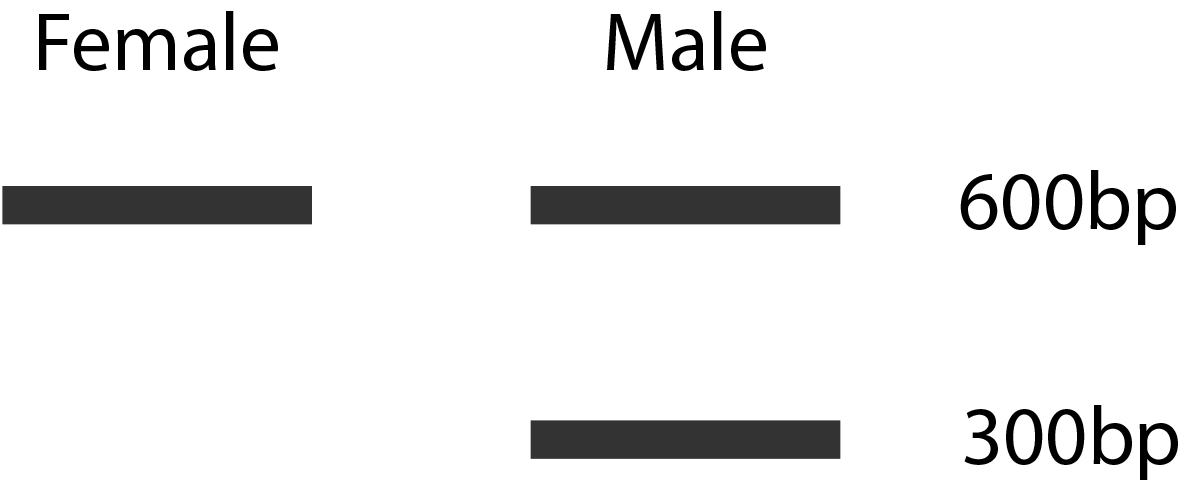
\includegraphics{05_Vertebrate_Experiment/../images/Sex_determ_gel_stickle.png}

}

\caption{Illustration of gel with female and male specific banding
patterns}

\end{figure}

\hypertarget{background-and-associated-papers}{%
\section{Background and associated
papers}\label{background-and-associated-papers}}

\hypertarget{sec-vert_exp-steroid_measure}{%
\chapter{Steroid Measurement}\label{sec-vert_exp-steroid_measure}}

\hypertarget{introduction-84}{%
\section{Introduction}\label{introduction-84}}

\begin{itemize}
\tightlist
\item
  \textbf{Purpose}: This procedure describes the technique of how to
  measure steroids in water that has been occupied by fish.
\item
  \textbf{Procedure Type}: Vert Experiment
\item
  \textbf{Species}:

  \begin{itemize}
  \tightlist
  \item
    Threespine stickleback, (\emph{Gasterosteus aculeatus}),
  \item
    Bay pipefish, (\emph{Syngnathus leptorhyncus}),
  \item
    Gulf pipefish (\emph{Syngnathus scovelli})
  \item
    Zebrafish, (\emph{Danio rerio}),
  \end{itemize}
\item
  \textbf{Author}: xxx
\item
  \textbf{Date Created}: xxx
\end{itemize}

\hypertarget{materials}{%
\section{Materials:}\label{materials}}

\begin{itemize}
\tightlist
\item
  150 ml glass beaker
\item
  C18 solid phase extraction (SPE) cartridges containing octadecylsilane
  (Sep-pak Plus, Waters Ltd., Watford, UK)
\end{itemize}

\hypertarget{solutions-71}{%
\section{Solutions}\label{solutions-71}}

\begin{itemize}
\tightlist
\item
  5 ml of distilled water
\item
  5 ml ethyl acetate
\item
  1 ml of RIA buffer (0.5 M phosphate buffer containing 0.2\% bovine
  serum albumen, 0.8\% sodium chloride, 0.03\% EDTA and 0.01\% sodium
  azide)
\item
  \textsuperscript{3}H-labeled steroids for 11-KT are purchased directly
  from Amersham Biosciences, UK (Scott et al., 2005)
\end{itemize}

\hypertarget{procedure-78}{%
\section{Procedure}\label{procedure-78}}

\hypertarget{water-collection}{%
\subsection{Water Collection}\label{water-collection}}

\begin{itemize}
\tightlist
\item
  The fish is placed in a 150-ml glass beaker with 50 ml of fresh water
  (the same source as used for aquaria) for 30 min.
\item
  In the case of male sticklebacks in individual tanks, the beaker is
  placed on a support in the tank to minimise the potential confinement
  stress.
\item
  After the 30-min period the fish is released in its tank.
\item
  If not able to pump the water sample immediately, pour the conditioned
  water into a 50-ml polypropylene centrifuge tube and store at 4°C (up
  to 1hour) or -20°C.
\end{itemize}

\hypertarget{steroid-extraction}{%
\subsection{Steroid Extraction}\label{steroid-extraction}}

\begin{itemize}
\tightlist
\item
  Water samples are pumped through C18 solid phase extraction (SPE)
  cartridges containing octadecylsilane (Sep-pak Plus, Waters Ltd.,
  Watford, UK).
\item
  The cartridges are first washed with 5 ml of 100\% methanol and then 5
  ml of distilled water.
\item
  As the volume of water is small (50ml) no filter is used.
\item
  The water samples are transferred into 60-ml syringes (BD Plastipak),
  drawn by vacuum through the cartridges, and 5 ml of distilled water is
  pushed through the cartridges and blown out.
\item
  The steroids are extracted with 5 ml ethyl acetate, which was then
  dried down to dryness under a stream of nitrogen (45°C).
\item
  Then, 1 ml of RIA buffer (0.5 M phosphate buffer containing 0.2\%
  bovine serum albumen, 0.8\% sodium chloride, 0.03\% EDTA and 0.01\%
  sodium azide) is added and the tubes stored at -20°C until RIAs.
\end{itemize}

\hypertarget{radioimmunoassay}{%
\subsection{Radioimmunoassay}\label{radioimmunoassay}}

\begin{itemize}
\tightlist
\item
  \textsuperscript{3}H-labeled steroids for 11-KT are purchased directly
  from Amersham Biosciences, UK (Scott et al., 2005).
\item
  Antisera came from previously recorded sources (see (Lower et al.,
  2004) where the same sort of study was carried out).
\item
  The RIA procedure has been described previously (Scott et al., 1980;
  Scott et al., 1984; Scott et al., 1982).
\item
  Briefly, 100 μl aliquots from the water sample extract or standards
  are transferred to assay tubes.
\item
  Labelled steroids and antisera are added in a further 100 μl of assay
  buffer, and the tubes left to incubate overnight at 4°C.
\item
  Free and bound labelled steroids are separated with dextran-coated
  charcoal by centrifugation (2,500 rpm for 12 min at 4ºC).
\item
  The supernatant is poured into suitable vials and 7 ml of
  scintillation fluid is added.
\item
  Each tube is then counted for 5 min in the counter (Beckman LS 6500).
\item
  The detection limit of the assays varied between 1 and 10 pg/ assay
  tube (i.e.~10 pg/ 100μl assay buffer).
\end{itemize}

\hypertarget{associated-papers-53}{%
\section{Associated Papers}\label{associated-papers-53}}

\begin{itemize}
\tightlist
\item
  LOWER, N., SCOTT, A. P. \& MOORE, A. (2004). Release of sex steroids
  into the water by roach. --- Journal of Fish Biology 64, 16-33.
\item
  SCOTT, A. P., BYE, V. J., BAYNES, S. M. \& SPRINGATE, J. R. C. (1980).
  Seasonal variations in plasma concentrations of 11-ketotestosterone
  and testosterone in male rainbow trout, Salmo gairdnerii Richardson.
  --- Journal of Fish Biology 17, 495-505.
\item
  SCOTT, A. P., SHELDRICK, E. L. \& FLINT, A.P.F. (1982). Measurement of
  17a,20b-dihydroxy-4-pregnen-3-one in plasma of trout (Salmo gairdneri
  Richardson): seasonal changes and response to salmon pituitary
  extract. --- General and Comparative Endocrinology 46, 444-451
\item
  SCOTT, A. P., MACKENZIE, D. S. \& STACEY, N. E. (1984). Endocrine
  changes during natural spawning in the white sucker, Catostomus
  commersoni. II. Steroid hormones. --- General and Comparative
  Endocrinology 56, 349-359.
\item
  SCOTT, A. P., PINILLOS, M. L. \& HUERTAS, M. (2005). The rate of
  uptake of sex steroids from water by Tinca tinca is influenced by
  their affinity for sex steroid binding protein in plasma. --- Journal
  of Fish Biology 67, 182-200
\end{itemize}

\hypertarget{sec-vert_exp-syngnathid_neuron}{%
\chapter{Pipefish backfill labeling if hindbrain
neurons}\label{sec-vert_exp-syngnathid_neuron}}

\hypertarget{introduction-85}{%
\section{Introduction}\label{introduction-85}}

\begin{itemize}
\tightlist
\item
  \textbf{Purpose}: This procedure descibes how to backfill nerons of
  pipefish.
\item
  \textbf{Procedure Type}: Experimental
\item
  \textbf{Species}:

  \begin{itemize}
  \tightlist
  \item
    Bay pipefish, (\emph{Syngnathus leptorhyncus})
  \item
    Gulf pipefish (\emph{Syngnathus scovelli})
  \end{itemize}
\item
  \textbf{Author}: Susie Bassham
\item
  \textbf{Date Created}: xxx
\end{itemize}

\hypertarget{materials-80}{%
\section{Materials}\label{materials-80}}

\begin{itemize}
\tightlist
\item
  Antibiotic (Cell Culture anti-biotic/mycotic from Gibco-BRL
  (15240-096) 100x Concentration) Stickleback embryo medium
\item
  Obsidian
\item
  Rhodamine
\item
  DiO lipophilic carbocyanine dye
\end{itemize}

\hypertarget{solutions-72}{%
\section{Solutions}\label{solutions-72}}

\begin{itemize}
\tightlist
\item
  MS-222 Anesthesia solution \{\#sec-husbandry\_anesth\_pipefish\}
\item
  MS-222 Euthanasia solution \{\#sec-vert\_husb-euthanasia\_syngnathid\}
\end{itemize}

\hypertarget{procedure-79}{%
\section{Procedure}\label{procedure-79}}

\begin{enumerate}
\def\labelenumi{\arabic{enumi}.}
\tightlist
\item
  Sedate Larval fish in MS222 in sterile filtered seawater + antibiotic
  (Cell Culture anti-biotic/mycotic from Gibco-BRL (15240-096) 100x
  Concentration).
\item
  Use a obsidian glass flake, an extremely sharp scalpel, an incision
  will be made from the dorsal side, extending ventrally just through
  the spinal cord.
\item
  Use a fine insect pin to apply dried crystals of rhodamine dextran,
  DiO, or similar reagent to the cut spinal cord.
\item
  Continuously sedate larvae. Euthanized with MS222 and fixed 5 to 16
  hours after surgery prior to imaging.
\end{enumerate}

\hypertarget{associated-papers-54}{%
\section{Associated Papers}\label{associated-papers-54}}

\begin{itemize}
\tightlist
\item
  xxx
\item
  xxx
\item
  xxx
\item
  xxx
\end{itemize}

\hypertarget{sec-vert_exp-live_alizarin_syngnathid}{%
\chapter{Live syngnathid alizarin
staining}\label{sec-vert_exp-live_alizarin_syngnathid}}

\hypertarget{introduction-86}{%
\section{Introduction}\label{introduction-86}}

\begin{itemize}
\tightlist
\item
  \textbf{Purpose}: This procedure describes how to live stain
  syngnathid with alizarin.
\item
  \textbf{Procedure Type}: Vert Experimental
\item
  \textbf{Species}:

  \begin{itemize}
  \tightlist
  \item
    Bay pipefish, (\emph{Syngnathus leptorhyncus})
  \item
    Gulf pipefish (\emph{Syngnathus scovelli})
  \end{itemize}
\item
  \textbf{Author}: Mark Currey
\item
  \textbf{Date Created}: January 01, 2024
\end{itemize}

\hypertarget{materials-81}{%
\section{Materials}\label{materials-81}}

\begin{itemize}
\tightlist
\item
  Large Petri Dish
\item
  xxx
\item
  xxx
\item
  xxx
\end{itemize}

\hypertarget{solutions-73}{%
\section{Solutions}\label{solutions-73}}

\begin{itemize}
\tightlist
\item
  Alizarin stock solutions: 0.5g Alizarin red in 100ml or in 50ml in
  sterile water (SIGMA cat\# A5533 Alizarin Red S, certified).
\item
  Staining Solution:

  \begin{itemize}
  \tightlist
  \item
    25 ppt Instant Ocean
  \item
    Add 10 ml 0.5\% or 1\% Alizarin Stock in sterile water for final
    concentrations of 0.005\% or 0.01\%.
  \item
    Adjust to pH 7.5 with NaOH
  \end{itemize}
\item
  For 50 ml (enough for 100mm diameter petri dish):

  \begin{itemize}
  \tightlist
  \item
    49.5 ml Embryo medium
  \item
    Add 500 µl 0.5\% or 1\% Alizarin Stock in sterile water
  \item
    Adjust to pH 7.5 with NaOH
  \end{itemize}
\item
  MESAB anesthesia strength \{\#sec-husbandry\_anesth\_pipefish\}
\item
  MESAB euthanisia strength \{\#sec-husbandry\_adult\_syng\_euth\}
\end{itemize}

\hypertarget{procedure-80}{%
\section{Procedure}\label{procedure-80}}

\begin{enumerate}
\def\labelenumi{\arabic{enumi}.}
\tightlist
\item
  Place fish into a container containing stain for 1-2 hours for larvae
  to overnight for juveniles or adult fish in the dark. We have found
  that fish do not experience adverse effects from being exposed to
  stain. Monitor fish every 30-60 minutes if possible. To de-stain,
  rinse thoroughly with embryo medium by placing fish into container of
  embryo medium without stain for 30 minutes; background continues to go
  down with time. Move on to DASPEI live staining if desired (see DASPEI
  live staining SOP) or anesthetize until the fish reaches a light plane
  of anesthesia (i.e.~movement has slowed down enough that the fish can
  be safely handled) and observe/image.
\item
  Bone fluorescence will decrease over time, so plan on imaging the same
  day if possible.
\item
  Keep fish in the dark as much as is reasonably convenient.
\item
  After fish has been observed/imaged place in a container of fish
  water. Monitor fish every 5-10 minutes until the fish is revived. Once
  fish is revived place back on the fish system and monitor during daily
  health checks. If the fish is to be fixed for post mortem experiments
  place fish directly into euthanasia MS222 solution and follow
  \{\#sec-husbandry\_adult\_syng\_euth\}.
\end{enumerate}

\hypertarget{associated-papers-55}{%
\section{Associated Papers}\label{associated-papers-55}}

\begin{itemize}
\tightlist
\item
  xxx
\item
  xxx
\item
  xxx
\item
  xxx
\end{itemize}

\hypertarget{sec-vert_exp-live_calcein_syngnathid}{%
\chapter{Live syngnathid calcein
staining}\label{sec-vert_exp-live_calcein_syngnathid}}

\hypertarget{introduction-87}{%
\section{Introduction}\label{introduction-87}}

\begin{itemize}
\tightlist
\item
  \textbf{Purpose}: This procedure describes how to live stain
  syngnathid with calcein.
\item
  \textbf{Procedure Type}: Vert Experimental
\item
  \textbf{Species}:

  \begin{itemize}
  \tightlist
  \item
    Bay pipefish, (\emph{Syngnathus leptorhyncus})
  \item
    Gulf pipefish (\emph{Syngnathus scovelli})
  \end{itemize}
\item
  \textbf{Author}: Mark Currey
\item
  \textbf{Date Created}: January 01, 2024
\end{itemize}

\hypertarget{materials-82}{%
\section{Materials}\label{materials-82}}

\begin{itemize}
\tightlist
\item
  Petri dishes and/or 1 L tanks
\item
  Calcein (Molecular Probes; cat. C481)
\end{itemize}

\hypertarget{solutions-74}{%
\section{Solutions}\label{solutions-74}}

\begin{itemize}
\tightlist
\item
  MESAB anesthesia strength \{\#sec-husbandry\_anesth\_pipefish\}
\item
  MESAB euthanisia strength \{\#sec-husbandry\_adult\_syng\_euth\}
\item
  25 ppt Instant Ocean
\item
  10\% NaOH
\item
  Stain Solution:

  \begin{itemize}
  \tightlist
  \item
    0.005 to 0.05\% calcein in sea water.
  \item
    Adjust pH to 8.2 with NaOH
  \item
    Make fresh, keep in dark.
  \end{itemize}
\end{itemize}

\hypertarget{procedure-81}{%
\section{Procedure}\label{procedure-81}}

\begin{enumerate}
\def\labelenumi{\arabic{enumi}.}
\tightlist
\item
  Place fish into a container containing stain for 1-2 hours for larvae
  to overnight for juveniles or adult fish in the dark. We have found
  that fish do not experience adverse effects from being exposed to
  stain. Monitor fish every 30-60 minutes if possible. To de-stain,
  rinse thoroughly with embryo medium by placing fish into container of
  embryo medium without stain for 30 minutes; background continues to go
  down with time. Move on to DASPEI live staining if desired (see DASPEI
  live staining SOP) or anesthetize until the fish reaches a light plane
  of anesthesia (i.e.~movement has slowed down enough that the fish can
  be safely handled) and observe/image.
\item
  Bone fluorescence will decrease over time, so plan on imaging the same
  day if possible.
\item
  Keep fish in the dark as much as is reasonably convenient.
\item
  After fish has been observed/imaged place in a container of fish
  water. Monitor fish every 5-10 minutes until the fish is revived. Once
  fish is revived place back on the fish system and monitor during daily
  health checks. If the fish is to be fixed for post mortem experiments
  place fish directly into euthanasia MS222 solution and follow the
  euthanasia SOP.
\end{enumerate}

\hypertarget{associated-papers-56}{%
\section{Associated Papers}\label{associated-papers-56}}

\begin{itemize}
\tightlist
\item
  xxx
\item
  xxx
\item
  xxx
\item
  xxx
\end{itemize}

\hypertarget{sec-vert_exp-live_daspei_syngnathid}{%
\chapter{Live syngnathid DASPEI
staining}\label{sec-vert_exp-live_daspei_syngnathid}}

\hypertarget{introduction-88}{%
\section{Introduction}\label{introduction-88}}

\begin{itemize}
\tightlist
\item
  \textbf{Purpose}: This procedure describes how to live stain
  syngnathid with DASPEI.
\item
  \textbf{Procedure Type}: Vert Experimental
\item
  \textbf{Species}:

  \begin{itemize}
  \tightlist
  \item
    Bay pipefish, (\emph{Syngnathus leptorhyncus})
  \item
    Gulf pipefish (\emph{Syngnathus scovelli})
  \end{itemize}
\item
  \textbf{Author}: Susie Bassham
\item
  \textbf{Date Created}: October 25, 2021; adapted from DOI:
  10.1007/s10162-002-3022-x
\end{itemize}

\hypertarget{materials-83}{%
\section{Materials}\label{materials-83}}

\begin{itemize}
\tightlist
\item
  Petri dishes and/or 1 L tanks
\item
  DASPEI (Sigma Aldrich; cat. D3418)
\end{itemize}

\hypertarget{solutions-75}{%
\section{Solutions}\label{solutions-75}}

\begin{itemize}
\tightlist
\item
  MESAB anesthesia strength \{\#sec-husbandry\_anesth\_pipefish\}
\item
  MESAB euthanisia strength \{\#sec-husbandry\_adult\_syng\_euth\}
\item
  25 ppt Instant Ocean
\item
  Staining Solution:

  \begin{itemize}
  \tightlist
  \item
    0.005\% DASPEI in sea water
  \end{itemize}
\end{itemize}

\hypertarget{procedure-82}{%
\section{Procedure}\label{procedure-82}}

\begin{enumerate}
\def\labelenumi{\arabic{enumi}.}
\tightlist
\item
  Stain larvae in Petri dishes and juveniles/adults in 1 L tanks
  containing stain solution for 5 to 75 min in the dark; stagger so that
  no fish stain longer than this before imaging. Rinse for 20 to 60 min
  in container of sea water without DASPEI to reduce background.
\item
  Keep fish in the dark as much as is reasonably convenient through
  procedures. Monitor fish every 15-30 minutes.
\item
  Anesthetize until the fish reaches a light plane of anesthesia
  (i.e.~movement has slowed down enough that the fish can be safely
  handled) and observe/image fluorescence immediately.
\item
  After fish has been observed/imaged place in a container of fish
  water. Monitor fish every 5-10 minutes until the fish is revived. Once
  fish is revived place back on the fish system and monitor during daily
  health checks. If the fish is to be fixed for post mortem experiments
  place fish directly into euthanasia MS222 solution and follow the
  euthanasia SOP.
\item
  Staining solution can be stored at 4C and reused.
\end{enumerate}

\hypertarget{associated-papers-57}{%
\section{Associated Papers}\label{associated-papers-57}}

\begin{itemize}
\tightlist
\item
  xxx
\item
  xxx
\item
  xxx
\item
  xxx
\end{itemize}

\hypertarget{sec-vert_exp-haploid_SB}{%
\chapter{Production of Haploid Embryos in
Stickleback}\label{sec-vert_exp-haploid_SB}}

\hypertarget{introduction-89}{%
\section{Introduction}\label{introduction-89}}

\begin{itemize}
\tightlist
\item
  \textbf{Purpose}: This method allows the production of homozygous
  haploid embryos for the purpose of screening for recessive mutations.
  Haploid embryos develop fairly normally for the first few days, but
  eventually develop bent tails and vacuolated body cavities. They are
  inviable.
\item
  \textbf{Procedure Type}: Vertabrate Experimental
\item
  \textbf{Species}:

  \begin{itemize}
  \tightlist
  \item
    Threespine stickleback, (\emph{Gasterosteus aculeatus})
  \end{itemize}
\item
  \textbf{Author}: Mark Currey
\item
  \textbf{Date Created}: xxx
\item
  \textbf{Date Updated}: xxx
\end{itemize}

This is a general procedure for making infertile sperm that can still
activate eggs for production of haploid, early pressure (EP) or heat
shock (HS) embryos.

\hypertarget{materials-84}{%
\section{Materials}\label{materials-84}}

\begin{itemize}
\tightlist
\item
  Watchglass
\item
  Large glass Petri dish
\item
  Ice
\item
  Two Pasteur pipettes
\item
  Pipette bulb
\item
  Stopwatch
\item
  UV Stratalinker® 1800 by Stratagene\\
\item
  Latex kitchen gloves
\item
  Safety glasses
\item
  Small test tube with cork marked for UV sperm
\end{itemize}

\hypertarget{solutions-76}{%
\section{Solutions}\label{solutions-76}}

\begin{itemize}
\tightlist
\item
  Hank's solution \{\#sec-general\_recipe\_hanks\}
\item
  xxx
\item
  xxx
\item
  xxx
\end{itemize}

\hypertarget{procedure-83}{%
\section{Procedure}\label{procedure-83}}

\begin{verbatim}
  1. Fill the bottom of the glass Petri dish with ice. 
  
  2. Put watchglass on top of the ice in the dish. 
  
  3. Using a Pasteur pipette, transfer the sperm from the test tube onto the watchglass. Be sure to get as much of the sperm into the pipette as possible without taking up any bubbles of air with it. Also, do not bubble the sperm in the watchglass as you are expelling them from the pipette. Expel sperm in a thin, even layer on watch glass.  
  
\end{verbatim}

\begin{tcolorbox}[enhanced jigsaw, rightrule=.15mm, title=\textcolor{quarto-callout-warning-color}{\faExclamationTriangle}\hspace{0.5em}{Warning}, titlerule=0mm, opacitybacktitle=0.6, toprule=.15mm, bottomrule=.15mm, opacityback=0, left=2mm, colframe=quarto-callout-warning-color-frame, breakable, coltitle=black, colback=white, colbacktitle=quarto-callout-warning-color!10!white, bottomtitle=1mm, leftrule=.75mm, toptitle=1mm, arc=.35mm]

DISCARD THIS PIPETTE.

\end{tcolorbox}

\begin{verbatim}
  4. Cover the sperm with the top of the Petri dish. 
  
  5. Put on the Latex gloves and safety glasses. 
  
  6. Place the covered Petri dish under the UV lamp. 
  
  7. Remove the cover of the Petri dish and start the stopwatch. 
  
  8. Gently move the dish under the lamp in a swirling motion for two minutes. 
  
  9. After exposing the sperm to UV light for two minutes, replace the cover on the Petri dish and remove the dish from under the lamp. 
  
  10. Using the CLEAN pipette, remove the sperm from the watchglass and transfer them to the small test tube marked for UV sperm. 
  
  11. Put the UV sperm test tube into the ice to be used later for fertilizing eggs.
\end{verbatim}

\hypertarget{associated-papers-58}{%
\section{Associated Papers}\label{associated-papers-58}}

\begin{itemize}
\tightlist
\item
  xxx
\item
  xxx
\item
  xxx
\item
  xxx
\end{itemize}

\hypertarget{sec-vert_exp-egg_storage_SB}{%
\chapter{Storage of stickleback
eggs}\label{sec-vert_exp-egg_storage_SB}}

\hypertarget{introduction-90}{%
\section{Introduction}\label{introduction-90}}

\begin{itemize}
\tightlist
\item
  \textbf{Purpose}: Storage of eggs for fertilization up to 24 hours
  post stripping.
\item
  \textbf{Procedure Type}: Vertabrate Experimental
\item
  \textbf{Species}:

  \begin{itemize}
  \tightlist
  \item
    Threespine stickleback, (\emph{Gasterosteus aculeatus})
  \end{itemize}
\item
  \textbf{Author}: Mark Currey
\item
  \textbf{Date Created}: xxx
\item
  \textbf{Date Updated}: xxx
\end{itemize}

This is a general procedure for making infertile sperm that can still
activate eggs for production of haploid, early pressure (EP) or heat
shock (HS) embryos.

\hypertarget{materials-85}{%
\section{Materials}\label{materials-85}}

\begin{itemize}
\tightlist
\item
  Streptomycin \& Penicillin Solution (PenStrep) from Sigma (P-0906)
  Stock -- 100\%
\item
  50ml sterile polypropylene conical tubes
\item
  90mm petri dish
\end{itemize}

\hypertarget{solutions-77}{%
\section{Solutions}\label{solutions-77}}

\begin{itemize}
\tightlist
\item
  Holtfrieter's Solution \{\#sec-general\_recipe\_holtfrieters\}
\item
  embryo medium \{\#sec-general\_recipe\_embryo\_medium\}
\item
  xxx
\item
  xxx
\end{itemize}

\hypertarget{procedure-84}{%
\section{Procedure}\label{procedure-84}}

\textbf{egg storage solution} 1. Add PenStrep to Holtfreiter's for a
final concentration of 1\% (10ml into 1 liter)

\begin{enumerate}
\def\labelenumi{\arabic{enumi}.}
\setcounter{enumi}{1}
\tightlist
\item
  Strip eggs from ripe female into a conical tube with 25ml cold egg
  storage solution.
\end{enumerate}

\begin{tcolorbox}[enhanced jigsaw, rightrule=.15mm, title=\textcolor{quarto-callout-note-color}{\faInfo}\hspace{0.5em}{Note}, titlerule=0mm, opacitybacktitle=0.6, toprule=.15mm, bottomrule=.15mm, opacityback=0, left=2mm, colframe=quarto-callout-note-color-frame, breakable, coltitle=black, colback=white, colbacktitle=quarto-callout-note-color!10!white, bottomtitle=1mm, leftrule=.75mm, toptitle=1mm, arc=.35mm]

Eggs can be transported on ice and fertilized up to 24 hours later
(maybe longer)

\end{tcolorbox}

\begin{enumerate}
\def\labelenumi{\arabic{enumi}.}
\setcounter{enumi}{2}
\item
  To fertilize, move eggs to 90mm petri dish and allow temperature to
  equilibrate to 20C
\item
  Remove egg storage solution, and rinse eggs once with embryo medium
  (important to make sure that salt concentration is low enough for
  sperm to be optimally activated).
\item
  Add macerated testis prep as usual, then cover eggs with embryo
  medium.
\end{enumerate}

\hypertarget{associated-papers-59}{%
\section{Associated Papers}\label{associated-papers-59}}

\begin{itemize}
\tightlist
\item
  xxx
\item
  xxx
\item
  xxx
\item
  xxx
\end{itemize}

\hypertarget{sec-vert_exp_CRISPR}{%
\chapter{CRISPR/Cas9 Technology}\label{sec-vert_exp_CRISPR}}

\hypertarget{introduction-91}{%
\section{Introduction}\label{introduction-91}}

\begin{itemize}
\tightlist
\item
  \textbf{Purpose}: This procedure describes CRISPR/Cas9 Technologies
  used in Threespine Stickleback.
\item
  \textbf{Procedure Type}: Vert Experiment
\item
  \textbf{Species}:

  \begin{itemize}
  \tightlist
  \item
    Threespine stickleback, (\emph{Gasterosteus aculeatus})
  \end{itemize}
\item
  \textbf{Author}: Sam Peterson and John H. Postlethwait, 2014, Modified
  by Susie 2/29/2024
\item
  \textbf{Date Created}: 2014
\end{itemize}

\begin{tcolorbox}[enhanced jigsaw, rightrule=.15mm, title=\textcolor{quarto-callout-note-color}{\faInfo}\hspace{0.5em}{CRISPR/Cas9 Technology}, titlerule=0mm, opacitybacktitle=0.6, toprule=.15mm, bottomrule=.15mm, opacityback=0, left=2mm, colframe=quarto-callout-note-color-frame, breakable, coltitle=black, colback=white, colbacktitle=quarto-callout-note-color!10!white, bottomtitle=1mm, leftrule=.75mm, toptitle=1mm, arc=.35mm]

This guide describes using the CRISPR/Cas9 system to induce small indels
or larger deletions in fish genomes. It includes descriptions of target
selection tools, generation and preparation of reagents, and mutation
screening approaches. Background information can be found in the
publications at the end of this protocol.

Introducing Cas9 enzyme and a guide RNA is used to cause double-stranded
breaks at a desired target locus in the genome. DNA repair machinery of
the cell seals the break, leaving a small insertion/deletion (indel) in
its place. In a coding region, this indel might result in a frame shift
that causes the remaining part of the mRNA to be translated incorrectly,
such as by generating an early stop codon, and this breaks the function
of the protein.

There are two ways to get Cas9 protein into cells. mRNA encoding Cas9
(particularly a version that has been codon adjusted to be translated
well in fish) can be injected. In that case, the cell's own translation
machinery uses this RNA to make Cas9 protein. It is economical to
generate large amounts of Cas9 RNA in vitro by using a plasmid carrying
the Cas9 gene driven by an RNA polymerase promoter (like the T3
promoter). The mRNA is then cleaned, quantified, aliquoted, and stored
at -80C until use. (This process is described below).

Alternatively, commercially purified Cas9 protein can be purchased in
lyophilized form and reconstituted into a liquid, aliquoted, and stored
at -80C until use. We have been using protein from PNA Bio
Inc.~(CP01-200 200 µg, that comes in four 50 µg aliquots). It arrives
lyophilized along with HEPES, KCl and sucrose so that adding 50 µl of
water to one of these aliquots reconstitutes the buffer at 1x and the
Cas9 at 1 mg/ml. Because we also sometimes co-inject guide RNAs with
plasmid knock-in constructs, we have adopted reconstituting in 50 µl of
1 mM DTT instead of pure water, to help prevent needle clogging. 1 µl
aliquots are frozen at -80C. For knock-in experiments, Cas9 protein
should be preferred over Cas9 mRNA, as it is believed maternal
homologous recombination machinery has a short window of opportunity,
during the one-cell stage (in other words, a delay due to Cas9 mRNA
needing to be translated can be avoided).

\end{tcolorbox}

\hypertarget{materials-86}{%
\section{Materials}\label{materials-86}}

\begin{itemize}
\tightlist
\item
  Injection rig
\item
  Needle puller
\item
\item
  xxx
\end{itemize}

\hypertarget{solutions-78}{%
\section{Solutions}\label{solutions-78}}

\begin{itemize}
\tightlist
\item
  xxx
\item
  xxx
\item
  xxx
\item
  xxx
\end{itemize}

\hypertarget{procedure-85}{%
\section{Procedure}\label{procedure-85}}

\begin{itemize}
\tightlist
\item
  \textbf{Generation of Cas9 mRNA (if not using Cas9 protein)}
\end{itemize}

\begin{tcolorbox}[enhanced jigsaw, rightrule=.15mm, title=\textcolor{quarto-callout-note-color}{\faInfo}\hspace{0.5em}{Note}, titlerule=0mm, opacitybacktitle=0.6, toprule=.15mm, bottomrule=.15mm, opacityback=0, left=2mm, colframe=quarto-callout-note-color-frame, breakable, coltitle=black, colback=white, colbacktitle=quarto-callout-note-color!10!white, bottomtitle=1mm, leftrule=.75mm, toptitle=1mm, arc=.35mm]

There are different plasmids available that can be used to transcribe
the Cas9 RNA. The one described in the Jao et al.~publication works
well. It is available from addgene: Plasmid 46757: pT3TS-nCas9n. Cas9
mRNA can be made by following the protocol outlined in their paper. The
plasmid is linearized with XbaI and used as a template after the
reaction is purified. mRNA is then synthesized with the T3 mMESSAGE kit
(Invitrogen) and cleaned with column purification.

Note: we should have aliquots frozen in strip tubes in the -80C, so it
is likely you will not need to make this yourself.

\end{tcolorbox}

\begin{verbatim}
1.  Grow 5ml of bacterial culture containing the pT3TS-nCas9n plasmid (stock located in -80° freezer box “CRISPR Reagents” in ampicillin overnight at 37°.  

2.  Extract plasmid DNA with the QIAprep Spin Miniprep Kit following manufacturer’s instructions. Measure concentration with the Qubit. 

3.  Linearize ~ 10 µg of plasmid with XbaI: 
                43 µl of plasmid DNA and water 
                5 µl NEB 10x buffer 
                2 µl XbaI 
                          
                Incubate overnight at 37C 

4. Clean the restriction reaction with Zymogen DNA Clean and Concentrator 5. At this point you can check the concentration with the Qubit and confirm complete linearization by running a small amount on a 1% agarose gel. There should be a single band at around 7 kb (7,330 bp). 

5. Make capped Cas9 mRNA with the mMESSAGE mMACHINE® T3 Transcription Kit following manufacturer’s instructions. Use about 1 µg of linearized plasmid DNA.  Note: unlike the original CRISPR/Cas9 zebrafish paper, the mRNA is not poly-adenylated with a separate step. Let the reaction go for 2 hours at 37° followed by the 15 minute optional DNAse step. 

6. Clean the reaction with Zymogen RNA Clean and Concentrator 25 and elute in 15-20 µl of nuclease free water. Check the size with 1µl on an agarose gel and measure the concentration with the nanodrop or with Qubit Broad Range RNA kit. 

7. Based on the measured concentration, dilute the remaining product to 200 ng/µl and store 3-4 µl aliquots at -80°C in the box labeled CRISPR reagents.  
\end{verbatim}

\textbf{Identify Target Sequence}

\begin{tcolorbox}[enhanced jigsaw, rightrule=.15mm, title=\textcolor{quarto-callout-note-color}{\faInfo}\hspace{0.5em}{Note}, titlerule=0mm, opacitybacktitle=0.6, toprule=.15mm, bottomrule=.15mm, opacityback=0, left=2mm, colframe=quarto-callout-note-color-frame, breakable, coltitle=black, colback=white, colbacktitle=quarto-callout-note-color!10!white, bottomtitle=1mm, leftrule=.75mm, toptitle=1mm, arc=.35mm]

The CRISPR/Cas9 system uses the injection of a guide RNA (gRNA) in
conjunction with Cas9 mRNA to create double-strand DNA breaks. Repair of
these dsDNA breaks with non-homologous end joining can result in indel
mutations or larger deletions spanning two simultaneously targeted
sites. The recognition sequence is specified by the gRNA and can be any
20 base pairs that are upstream from NGG. Efficient transcription using
a T7 promoter requires the transcript start with GG. This limits the
possible recognition sites to GG-(N)18-NGG. This can be relaxed to
G-(N)19-NGG if necessary and transcription of these are usually not
problematic. The orientation of the target sequence relative to a target
gene is not important so sense and anti-sense strands can be searched.
Please note that the NGG at the end of the recognition sequence is not
considered part of the target site and will not be incorporated into the
transcribed gRNA.

Online tools for designing CRISPR targets come and go. Their criteria
for scoring prospective targets differ and the different platforms will
often identify non-overlapping sets of targets, or they may rank the
same sites very differently. Some tools are able to take into account
potential off-target sites in the stickleback genome.

These two sites support many species including stickleback (i.e.,
includes a search of off-target sites). CCtop:
https://cctop.cos.uni-heidelberg.de/species.html and ChopChop:
http://chopchop.cbu.uib.no

CrisprScan currently supports zebrafish, medaka and killifish but not
stickleback, however its algorithm is based on significant empirical
testing and appears to perform well:
https://www.crisprscan.org/sequence/

\end{tcolorbox}

\begin{verbatim}
1. To use these tools, paste in a DNA sequence that you want to search for potential target sites (e.g., an early exon or flanking region).   

2. Select the T7 promoter to identify target sequences starting with GG. Select the stickleback genome (this is used to check for off-target regions), or in CrisprScan select “No search” (because otherwise the default is zebrafish). 

Tools like CrisprScan will also select targets that might start with GN or NG, in which case it will suggest changing the N to a G. This mismatch will be OK for targeting, and will allow better guide synthesis using T7 RNA polymerase. When generating annotations of your chosen targets in your reference sequence file of the genomic region, it is helpful to designate the orientation of the annotated target (either + or -). 

3. Using target sequences with multiple alignments to the genome or close matches may result in unwanted off-target effects. Use BLAT at https://genome.ucsc.edu/cgi-bin/hgBlat to compare your selected 20 base pair target sequence/s to the stickleback genome to confirm it matches only a single time and BLAT to the human genome to check that there are no matches (relevant to biosafety concerns). If the design tool recommended changing one of the start nucleotides to a G, BLAT the sequence that includes that change in addition to the original genomic target sequence.  

4. If you are using an Oregon stickleback source population, you can and should blast and compare the region of interest against an Oregon reference genome (like Cushman Slough) to confirm there are no polymorphisms in the targets you have selected, as these can reduce obliterate their efficacy. Alternatively, you could amplify the region of interest in the line /source population you are using and Sanger sequence it to ensure your designed target is identical. 
\end{verbatim}

\begin{tcolorbox}[enhanced jigsaw, rightrule=.15mm, title=\textcolor{quarto-callout-note-color}{\faInfo}\hspace{0.5em}{Important Consideration}, titlerule=0mm, opacitybacktitle=0.6, toprule=.15mm, bottomrule=.15mm, opacityback=0, left=2mm, colframe=quarto-callout-note-color-frame, breakable, coltitle=black, colback=white, colbacktitle=quarto-callout-note-color!10!white, bottomtitle=1mm, leftrule=.75mm, toptitle=1mm, arc=.35mm]

Important consideration: even when single guide RNAs work well, a
functional protein might still be produced. For example, if an indel
generated is a multiple of 3 bp, it could delete or add a small number
of codons (and therefore amino acids) while not disrupting the reading
frame for the rest of the coding region. Such mutations might not
abolish or possibly even affect the function of the protein. In order to
help circumvent this and also to make it easier to screen indels by size
on an electrophoresis gel, design a pair of target sequences that can be
injected at the same time to create a larger deletion. Successfully
deleted alleles will be easily resolved when PCR products flanking the
region are run on a gel. On the other hand, indels produced by a single
gRNA might not be discernable from wild type on a gel. Indels will be
created around the site of the double-strand break, which will occur
three base pairs before the NGG; so, if only a single guide will be used
for some reason, you can try to design a single target sequence that
would disrupt a restriction enzyme recognition sequence when an indel is
created in the expected location. In that case, screening is a two-step
process: amplify a fragment around the predicted indel, then try to
digest the fragment with the restriction enzyme. Wildtype fragments will
be cut, fragments with the indel will not be cut. And, if you've
designed the positions of your primers well, you can resolve all three
fragment sizes on a gel. Alternatively, PCR products can be Sanger
sequenced -- an expensive way to screen large numbers of prospective
CRISPR mutants.

\end{tcolorbox}

\textbf{Create gRNA DNA template}

\begin{tcolorbox}[enhanced jigsaw, rightrule=.15mm, title=\textcolor{quarto-callout-note-color}{\faInfo}\hspace{0.5em}{Notes}, titlerule=0mm, opacitybacktitle=0.6, toprule=.15mm, bottomrule=.15mm, opacityback=0, left=2mm, colframe=quarto-callout-note-color-frame, breakable, coltitle=black, colback=white, colbacktitle=quarto-callout-note-color!10!white, bottomtitle=1mm, leftrule=.75mm, toptitle=1mm, arc=.35mm]

There are multiple methods described for producing gRNA templates. The
standard method described in initial publications involves annealing two
small oligos and ligating them into a cut vector which is then cloned. I
prefer a simpler method which is adapted from one published in Cell
Reports (Bassett et al., 2013). It involves using two long oligos in a
template-free PCR reaction. The two oligos will partially anneal to each
other and the polymerase will fill in the rest yielding a short
double-stranded template with a T7 recognition site. One oligo is
generic in that it is used in every template production reaction. The
other is sequence specific to the target sequence. It should provide
essentially the same template as if you were to use the cloning method
described in Jao et al., 2013 with the addgene plasmid 46759: pT7-gRNA
(the last few nucleotides on the 3 prime end may be different, but these
do not seem to matter). This is then used as a template for in vitro
transcription. Once the base components are obtained, the only
additional thing that needs to be ordered for new targets is the gene
specific oligo.

\end{tcolorbox}

\begin{verbatim}
1. Obtain gRNA scaffold oligo (PAGE purified). IDT provides this service for their Ultramer DNA Oligos. A single order should provide enough for at least 100 template synthesis reactions.  
\end{verbatim}

\begin{tcolorbox}[enhanced jigsaw, rightrule=.15mm, title=\textcolor{quarto-callout-note-color}{\faInfo}\hspace{0.5em}{Notes}, titlerule=0mm, opacitybacktitle=0.6, toprule=.15mm, bottomrule=.15mm, opacityback=0, left=2mm, colframe=quarto-callout-note-color-frame, breakable, coltitle=black, colback=white, colbacktitle=quarto-callout-note-color!10!white, bottomtitle=1mm, leftrule=.75mm, toptitle=1mm, arc=.35mm]

We have a lab stock of this oligo and you should not need to order it.

\end{tcolorbox}

5\texttt{-gatccgcaccgactcggtgccactttttcaagttgataacggactagccttattttaacttgctatttctagctctaaaac-3}

\begin{verbatim}
2. Order gene-specific oligo. In our hands, this oligo does not need to be PAGE purified. The sequence should be [T7 promoter]-[Target Sequence]-[start of gRNA sequence]. Note: CrisprScan provides a version of this sequence, though it is shorter by a few nucleotides at either end – it probably also works, but the Cresko lab uses the slightly extended sequence below. 
\end{verbatim}

5\texttt{-\ aattaatacgactcactata-{[}20\ nt\ Target\ Sequence{]}-gttttagagctagaaatagc-3}

\begin{tcolorbox}[enhanced jigsaw, rightrule=.15mm, title=\textcolor{quarto-callout-note-color}{\faInfo}\hspace{0.5em}{Notes}, titlerule=0mm, opacitybacktitle=0.6, toprule=.15mm, bottomrule=.15mm, opacityback=0, left=2mm, colframe=quarto-callout-note-color-frame, breakable, coltitle=black, colback=white, colbacktitle=quarto-callout-note-color!10!white, bottomtitle=1mm, leftrule=.75mm, toptitle=1mm, arc=.35mm]

Note: do not include the NGG (the PAM sequence).

Note: if your target is on the minus strand, make sure to reverse
complement the target sequence before plugging into this sequence above.
In other words, the end facing the NGG should be to the right.

Note: If you haven't selected a target that already starts with GG, the
design software will probably have suggested that targets starting with
NG or GN should be changed to GG. Don't forget to include this suggested
change, supporting better T7 transcription.

\end{tcolorbox}

\begin{verbatim}
3. Perform PCR. The two oligos serves both as primers and template. Phusion polymerase is recommended but other polymerases should work as well. 

        - 4µl 5x Buffer 
        - 0.4µl dNTPs (10 mM) 
        - 1 µl of gene specific oligo (10 µM) 
        - 1 µl of gRNA scaffold oligo (10 µM) 
        - 0.2 µl Phusion 
        - 13.4 µl Water 
        
         98° 30 seconds 
         
         40 cycles of:  
         98° 10 seconds 
         60° 10 seconds 
         72° 15 seconds 
         72° 10 mins 

 

4. Clean the PCR reaction with column-based method (e.g., Zymo DNA Clean and Concentrator kit) or at least 2.5x volume of Omega beads (SB). At this point, the concentration can be checked and the product can be analyzed on a gel. It should be a single 125 bp band. [Susie adds: With Zymo columns, eluting in 20 µl, this reaction yields about 25 ng/µl. For short templates, the Megascript kit recommends using 100-200 ng per reaction. So for a half reaction, you would use 2-4 µl of the PCR product]. 

5. Use as template for in vitro transcription with either, MAXIscript® T7 Kit or MEGAscript® T7 Kit, both by Invitrogen. Perform the optional DNAse step and clean with column based method. Both kits should produce enough RNA. However, the MEGAscript T7 Kit will produce much more. I prefer using 4 µl of the template in a half reaction of the MEGAscript T7 Kit. The reaction can be extended for several hours or overnight to increase yield if necessary. After column based purification, it usually provides around 1 µg/µl in a 25µl elution but this can be quite variable. The RNA can be checked on a gel, but the results can be difficult to interpret due to heavy secondary structure. It usually looks like one or two bands around 100 and 200 bp. 

 
\end{verbatim}

\textbf{Inject Cas9 mRNA and gRNA into one-celled embryos}

\begin{tcolorbox}[enhanced jigsaw, rightrule=.15mm, title=\textcolor{quarto-callout-note-color}{\faInfo}\hspace{0.5em}{Notes}, titlerule=0mm, opacitybacktitle=0.6, toprule=.15mm, bottomrule=.15mm, opacityback=0, left=2mm, colframe=quarto-callout-note-color-frame, breakable, coltitle=black, colback=white, colbacktitle=quarto-callout-note-color!10!white, bottomtitle=1mm, leftrule=.75mm, toptitle=1mm, arc=.35mm]

Embryos should be injected at the one cell stage according to standard
protocols. Briefly, as soon as feasible, separate and clean fertilized
embryos and, in filter sterilized embryo medium, load them into the
grooves milled into a plastic insert fitting in a square plastic dish.
They need to be held securely but do not necessarily have to be pushed
to the bottom of the groove. Eggs from different clutches can differ in
diameter; choose the width of the milled groove and depth of embryos
within the groove to hold them without applying too much compression.
The blastomere should be oriented up or slightly tilted toward the
direction of the injection needle. A high concentration of Cas9 mRNA
(2nl of 300 ng/µl as suggested in early papers) can cause mortality
(reported by JHP lab). Lower concentrations (100 ng/µl or lower) seem to
be just as effective and cause less developmental defects and death. The
gRNA concentration does not seem to matter as much (reported
concentrations range greatly, from 1 ng/µl to almost 100 ng/µl). Higher
concentrations of gRNA do not seem to cause any additional defects or
mortality. I recommend starting at 100 ng/µl Cas9 with 50 ng/µl gRNA. If
mutagenesis is not detected with these concentrations than check the RNA
prep or consider that there may be a problem with the target location.
Some target sites do not work as well as others. Additionally, it is
useful to sequence the target region in the fish being used for
injections to confirm that the reference genome sequence is accurate. If
mutagenesis rates are successful, then the injection concentrations can
be changed based on mortality/deformity percentages and mutation
efficiency. The gRNA concentration can likely be lowered significantly
without affecting efficiency. Checking potential off-targets is advised
as well and might influence the ideal injection concentrations. If a
positive control is desired, the fh (second target site) gRNA described
in Hwang et al.~works at a high level of efficiency.

\end{tcolorbox}

\textbf{Inject embryos}

\emph{If using Cas9 mRNA}

\begin{verbatim}
1. On ice, prepare injection mixture in water with 1/10 volume phenol red*: 
  
  100 ng/µl Cas9 mRNA (range 50 to 100 ng/µl) 
  50 ng/µl gRNA (use 50 ng/µl of each gRNA if targeting multiple sites) 
\end{verbatim}

\textbf{If using Cas9 protein}

\begin{verbatim}
2. To preload protein, mix in these final concentrations (according the PNA Bio recommendations for zebrafish**): 
  
  500 ng/µl Cas9 protein (range: about 200-800 ng/µl) 
  250 ng/µl gRNA (range: about 100-400 ng/µl) 
  Incubate for 5’ at 37C then put on ice. 
  Add 1/10 volume phenol red* 
\end{verbatim}

\begin{tcolorbox}[enhanced jigsaw, rightrule=.15mm, title=\textcolor{quarto-callout-note-color}{\faInfo}\hspace{0.5em}{Notes}, titlerule=0mm, opacitybacktitle=0.6, toprule=.15mm, bottomrule=.15mm, opacityback=0, left=2mm, colframe=quarto-callout-note-color-frame, breakable, coltitle=black, colback=white, colbacktitle=quarto-callout-note-color!10!white, bottomtitle=1mm, leftrule=.75mm, toptitle=1mm, arc=.35mm]

*Note: before thawing your other reagents, thaw and vortex the phenol
red stock. Centrifuge the tube at max speed for 10 minutes to pellet any
needle-clogging precipitate before adding some to your other injection
reagents.

**Note: the reason for these ranges is that different targets work with
different efficiencies. Also, you might be constrained in final
concentrations if, for example, you want to use more than one guide in
combination, as the volume of each reagent you add dilutes the
constituents.

\end{tcolorbox}

\begin{verbatim}
3. Inject into the cell at the one-cell stage (1-2 nl). 
\end{verbatim}

\textbf{Screen Embryos for Mutations}

::: \{.callout-note title=``Notes''\} Large deletions induced by using
multiple gRNAs can be screened for with PCR. Mutagenesis in the form of
induced indels can be detected with either the Restriction Fragment
Length Polymorphism (RFLP) assay, or by Sanger sequencing of amplicons.
The RFLP assay detects changes in a restriction enzyme recognition
sequence. Sanger sequencing amplicons from injected embryos can detect
mosaicism at the target site. Screening 48 hpf embryos that appear to be
developmentally normally provides a good measure of whether or not
mutations were induced and to what degree. Later stages that are
developing abnormally and would not survive anyway can also be
euthanized and screened. Uninjected siblings should always be used as
negative controls.\\
:::

\textbf{Lysis-based DNA prep (this provides DNA that is not clean but
accessible enough for PCR)}

\begin{verbatim}
  1. Collect and euthanize embryos according to standard protocols (individuals or in groups of up to 5). If they are still in chorions, they should be crushed with a blue plastic pestle or chorions can be poked or crushed with sharp foreceps. 
  
  2. Remove water and lyse embryos with HotShot method (Meeker et al. 2007) 
  
  3. Add 100 µl of 50mM NaOH (50 µl for an individual embryo) 
  
  4. Heat at 95° for 20 mins 
  
  5. Chill on ice and neutralize with 10ul of 1 M Tris-HCl, pH 8.0 (5 µl for an individual embryo) 
\end{verbatim}

\textbf{RFLP Assay}

::: \{.callout-note title=``Notes''\} This assay only works if there is
a unique restriction enzyme recognition sequence located around the 3`
end of the target sequence. If the recognition sequence is altered by
successful mutagenesis, the restriction enzyme will no longer be able to
cut the PCR product.\\
:::

\begin{verbatim}
1. Perform PCR (look to amplify a 300-600 bp amplicon surrounding expected mutation site), preferably with the indel location positioned off-center with respect to the expected amplicon so that two different fragment lengths will be produced after cutting 

2. Run 2 µl of reaction on a gel to confirm a single band at the proper length 

3. Clean the PCR reaction with preferred method and cut with the appropriate restriction enzyme. For many restriction enzymes, purification of the reaction is not necessary. 

4. Run the reaction on a gel to determine if the restriction enzyme recognition site was altered. Results from uninjected embryos should show a completely digested product. Successful mutagenesis can be qualitatively estimated by looking at the intensity of the undigested PCR product. 
\end{verbatim}

\textbf{Sanger Sequencing}

\begin{verbatim}
1. Perform PCR (look to amplify a 300-600 bp amplicon surrounding expected mutation site). Run some of the reaction on a gel to confirm a correct sized product was amplified. 

2. Clean the rest of the reaction with preferred reaction clean-up method, elute in 50 µl, and send the reaction out for Sanger sequencing. The concentration can be measured at this point (although usually 1 µl is sufficient for Sanger sequencing).     

3. Send the PCR products to Genewiz according to their recommendations. 

4. Analyze results to estimate mutagenesis efficiency. It is not very useful to look at the actual sequence that is returned. It is much more informative to look at the trace file with the actual peaks. 

5. Results from uninjected embryos should be very clean with a single peak at each nucleotide position. Occasionally there will be two peaks for one nucleotide when the individual carried a polymorphism. It is also recommended to confirm that the fish do not carry polymorphisms in the target sequence region as this could drastically lower or abolish mutagenesis efficiency. 

6. Sequencing results from injected embryos should show nice clean peaks until near the target region where the quality should dramatically drop off (see attached trace image). 

7. There are online tools (e.g., https://tide.nki.nl/#about) to try to algorithmically disentangle the alleles present and their predicted frequencies in the mosaic fish from this kind of  sequence trace file (also called a chromatogram). 
\end{verbatim}

\st{Insert image if sequence here}

\begin{itemize}
\tightlist
\item
  Sequence from successful mutagenesis attempt
\end{itemize}

\textbf{F1 Screening}

::: \{.callout-note title=``Notes''\} The goal of using CRISPR/Cas9 is
to obtain a stable mutant line. Injected fish should be considered
potential mosaic carriers of mutations at the target region. Some cells
will contain the unmutated wild-type sequence while other cells will
carry mutations. Also to be noted is that different cells will contain
different mutations. By outcrossing potential carriers, stable
heterozygous mutant carriers can be obtained and identified.

The process of obtaining F1 carriers can be split into a few steps.
Below lists the key steps followed by a brief explanation of options and
thoughts on how to minimize the time to obtain mutants, cost of
screening, number of tanks used and effort required. :::

\begin{verbatim}
1. Outcross injected fish to wildtype background. 

2. Screen outcrossed clutches to estimate efficiency of mutation inheritance.  

3. Raise clutch that has decent inheritance efficiency. 

4. Fin clip potential F1 carriers and identify carriers. 

5. Sequence mutation carriers to determine exact molecular nature of mutation. 

6. Select fish who carry a desirable mutation. 
\end{verbatim}

\begin{tcolorbox}[enhanced jigsaw, rightrule=.15mm, title=\textcolor{quarto-callout-note-color}{\faInfo}\hspace{0.5em}{Notes}, titlerule=0mm, opacitybacktitle=0.6, toprule=.15mm, bottomrule=.15mm, opacityback=0, left=2mm, colframe=quarto-callout-note-color-frame, breakable, coltitle=black, colback=white, colbacktitle=quarto-callout-note-color!10!white, bottomtitle=1mm, leftrule=.75mm, toptitle=1mm, arc=.35mm]

\begin{enumerate}
\def\labelenumi{\arabic{enumi}.}
\item
  Usually, 25 injected fish are put into the fry rack and raised to
  adulthood. Sometimes the injections cause developmental delays or
  issues that impact initial survival. In these cases, more than 25 fish
  can be put into the nursery. However, there isn't a significant
  advantage raising more than 1 tank of injected fish. Injected fish
  should carry mutations at reasonable rates. If 25 fish are screened
  and none of them pass on a mutation the problem is better resolved by
  re-injecting at a higher concentration or using a different target
  site. When the fish reach a breedable age, 3 or 4 fish should be
  pairwise mated with wildtype stocks. These clutches should be kept
  separate so inheritance efficiency can be measured.
\item
  Out-crossed fish will be raised to adulthood before they are IDd and
  the exact molecular nature of the mutation is determined. This takes
  several months and takes up tank space. Screening clutches to estimate
  inheritance efficiency is recommended to avoid 2 things: 1) the need
  to raise several tanks of different clutches to insure that a mutant
  carrier is obtained 2) wasting several months waiting for fish to grow
  to find out that none of them carry a mutation.
\item
  Raise 25 fish from 1 or 2 clutches of F1 fish to adulthood. These
  should be selected based on the initial clutch screening. The F0 fish
  should be maintained until a stable line is obtained. Inheritance
  efficiency of individual clutches can be estimated by testing siblings
  by PCR (to detect a large deletion or via RFLP if there is an
  appropriate restriction enzyme site. Fish that are not carriers of
  mutations will give a PCR product that is completely digested by the
  restriction enzyme while those that carry a mutation will show a
  prominent undigested band.
\item
  Sanger sequencing of amplicons from carriers is used to determine the
  exact nature of the mutation. This is important for several reasons 1)
  not all mutations are predicted to cause a loss-of-function (it is
  important that the mutation causes a frame-shift or early termination
  codon) 2) knowing the exact nature of the mutation is important for
  developing a genotyping protocol and reporting results. There are a
  few options for how to do this. The PCR product from identified
  carriers can be cloned and then sequenced. This gives an easy to read
  result but is slightly costly and time consuming. The other option is
  to directly sequence the PCR products without cloning. This is easier
  and more cost effective but requires some effort to determine the
  mutation.
\end{enumerate}

Unlike the results of injected embryos which potentially carry many
different alleles, the F1 carriers should be wildtype or should be
heterozygous with one wildtype and one mutant allele if they are
carriers. If the sequence is clean throughout (or the trace file shows
only, e.g., a naturally occurring SNP), then the fish is not a carrier.
If the sequence starts clean but then turns into a series of double and
sometimes single peaks, then the fish is likely a carrier of an indel
mutation. Since the WT sequence is known, the sequence of the mutation
can be read by ``subtracting'' the WT peaks (if at a given nucleotide
position the WT sequence is expected to be A and there is a peak for A
and T, then the mutant allele has a T at that position -- if there is a
single peak, then both the mutant and WT sequence has the same
nucleotide at that position). See picture. Again, there are online tools
to disentangle the WT and mutant allele sequences
(https://tide.nki.nl/\#about).

\st{insert image here}

\begin{enumerate}
\def\labelenumi{\arabic{enumi}.}
\setcounter{enumi}{5}
\tightlist
\item
  It is likely that screening 1 or 2 clutches of F1 fish will produce
  multiple carriers of different mutations. At this point a decision
  must be made at which fish should be kept. It is advantageous to have
  multiple alleles of a mutation so that a phenotype can be confirmed.
  However, saving more than 2 alleles increases tank usage but doesn't
  offer that much of an advantage. It is helpful when a male and a
  female carrier of the same allele are identified so that they can be
  bred to obtain a homozygous mutant without having to have an
  additional outcross generation.
\end{enumerate}

\end{tcolorbox}

\hypertarget{associated-papers-60}{%
\section{Associated Papers}\label{associated-papers-60}}

\begin{verbatim}
- Efficient genome editing in zebrafish using a CRISPR-Cas system. (Hwang et al., 2013)
- Efficient multiplex biallelic zebrafish genome editing using a CRISPR nuclease system. (Jao et al., 2013). 
- crisPrscan: designing highly efficient sgrnAs for crisPr-cas9 targeting in vivo (Moreno-Mateos et al., 2015). 
- Maximizing mutagenesis with solubilized Crispr-Cas9 ribonucleoprotein complexes (Burger et al., 2017). 
- A simple and effective F0 knockout method for rapid screening of behavior and other complex phenotypes (Kroll et al., 2022). 
\end{verbatim}

\part{Daphnia Husbandry}

This section of the manual contains protocols for the safe and ethical
husbandry and use of invertebrate animals, particular the nematode worm
\emph{C. remanei} and water fleas of the genus \emph{Daphnia}

\hypertarget{sec-Daphnia}{%
\chapter{Placeholder\_Daphnia}\label{sec-Daphnia}}

\hypertarget{xxx-2}{%
\section{xxx}\label{xxx-2}}

xxxx

\hypertarget{xxx-3}{%
\subsection{xxx}\label{xxx-3}}

xxxxx

\part{Common Recipes}

This section of the book contains common recipes used for solutions and
reagents across other protocols

\hypertarget{sec-recipe-dietrichs_fix}{%
\chapter{Dietrich's Fixative (EM)}\label{sec-recipe-dietrichs_fix}}

\hypertarget{introduction-92}{%
\section{Introduction}\label{introduction-92}}

\begin{itemize}
\tightlist
\item
  \textbf{Purpose}: Recipe for Dietrich's fixative
\item
  \textbf{Procedure Type}: recipe
\item
  \textbf{Species}:

  \begin{itemize}
  \tightlist
  \item
    Threespine stickleback, (\emph{Gasterosteus aculeatus})
  \item
    Bay pipefish, (\emph{Syngnathus leptorhyncus})
  \item
    Gulf pipefish (\emph{Syngnathus scovelli})
  \end{itemize}
\item
  \textbf{Author}: Mark Currey
\item
  \textbf{Date Created}: February 29, 2024
\end{itemize}

When fixing sentinel fish use Dieterich's fixative.

\hypertarget{materials-87}{%
\section{Materials}\label{materials-87}}

\begin{itemize}
\tightlist
\item
  Ethanol (95\%)
\item
  Formalin (Formaldehyde 37\% solution, histological grade, contains
  10-15\% methanol, Sigma \# F1635)
\item
  Glacial Acetic Acid
\item
  Distilled WaterSolutions
\end{itemize}

\hypertarget{procedure-86}{%
\section{Procedure}\label{procedure-86}}

\begin{enumerate}
\def\labelenumi{\arabic{enumi}.}
\tightlist
\item
  Prepare Dietrich's Fixative (100 ml), mix: - 30 ml Ethanol (95\%) - 10
  ml Formalin (Formaldehyde 37\% solution, histological grade, contains
  10-15\% methanol, Sigma \# F1635) - 2 ml Glacial Acetic Acid - 58 ml
  Distilled Water
\item
  Store fixative at room temperature.
\end{enumerate}

\hypertarget{associated-papers-61}{%
\section{Associated Papers}\label{associated-papers-61}}

\begin{itemize}
\tightlist
\item
  xxx
\item
  xxx
\item
  xxx
\item
  xxx
\end{itemize}

\hypertarget{sec-recipe-em}{%
\chapter{Stickleback Embryo Medium (EM)}\label{sec-recipe-em}}

\hypertarget{introduction-93}{%
\section{Introduction}\label{introduction-93}}

\begin{itemize}
\tightlist
\item
  \textbf{Purpose}: Recipe for embryo medium\\
\item
  \textbf{Procedure Type}: recipe
\item
  \textbf{Species}:

  \begin{itemize}
  \tightlist
  \item
    Threespine stickleback, (\emph{Gasterosteus aculeatus})
  \end{itemize}
\item
  \textbf{Author}: Mark Currey
\item
  \textbf{Date Created}: January 1, 2004
\end{itemize}

\hypertarget{materials-88}{%
\section{Materials}\label{materials-88}}

\begin{itemize}
\tightlist
\item
  Instant Ocean Salt
\item
  Baking Soda
\item
  nano pure water (npH2O)
\end{itemize}

\hypertarget{solutions-79}{%
\section{Solutions}\label{solutions-79}}

\begin{itemize}
\tightlist
\item
  none
\end{itemize}

\hypertarget{procedure-87}{%
\section{Procedure}\label{procedure-87}}

For 2 liters: 1. Add 8g Instant Ocean to 2 liters of npH2O 2. Add
\textasciitilde0.5g baking soda 3. Check pH and adjust to 7.0 -- 8.0

Salt and baking soda are located in containers near the weigh station.
Rinse 2 liter flasks with DI water between uses.

\hypertarget{associated-papers-62}{%
\section{Associated Papers}\label{associated-papers-62}}

\begin{itemize}
\tightlist
\item
  xxx
\item
  xxx
\item
  xxx
\item
  xxx
\end{itemize}

\hypertarget{sec-recipe-ginzbergs_ringers}{%
\chapter{Ginzberg's Ringer
Solution}\label{sec-recipe-ginzbergs_ringers}}

\hypertarget{introduction-94}{%
\section{Introduction}\label{introduction-94}}

\begin{itemize}
\tightlist
\item
  \textbf{Purpose}: Recipe for making ginzberg's ringers solution\\
\item
  \textbf{Procedure Type}: recipe
\item
  \textbf{Species}:

  \begin{itemize}
  \tightlist
  \item
    Threespine stickleback, (\emph{Gasterosteus aculeatus})
  \end{itemize}
\item
  \textbf{Author}: Mark Currey
\item
  \textbf{Date Created}: January 1, 2004
\end{itemize}

\hypertarget{materials-89}{%
\section{Materials}\label{materials-89}}

\begin{itemize}
\tightlist
\item
  NaCl
\item
  KCl
\item
  CaCl2
\item
  NaHCO3
\item
  npH2O
\end{itemize}

All of these reagents should be located in the chemical cabinet.

\hypertarget{solutions-80}{%
\section{Solutions}\label{solutions-80}}

\begin{itemize}
\tightlist
\item
  none
\end{itemize}

\hypertarget{procedure-88}{%
\section{Procedure}\label{procedure-88}}

For 1000 mls, mix: 1. Mix solids into 750 ml of npH2O - 6.6g NaCl -
0.25g KCl - 0.3g CaCl2 - 0.2g NaHCO3 2. Bring to 1 liter total volume
with npH2O. 3. Store at 4° C.

\hypertarget{associated-papers-63}{%
\section{Associated Papers}\label{associated-papers-63}}

\begin{itemize}
\tightlist
\item
  xxx
\item
  xxx
\item
  xxx
\item
  xxx
\end{itemize}

\hypertarget{sec-recipe-mesab}{%
\chapter{Mesab Stock (EM)}\label{sec-recipe-mesab}}

\hypertarget{introduction-95}{%
\section{Introduction}\label{introduction-95}}

\begin{itemize}
\tightlist
\item
  \textbf{Purpose}: Recipe for making a mesab stock solution\\
\item
  \textbf{Procedure Type}: recipe
\item
  \textbf{Species}:

  \begin{itemize}
  \tightlist
  \item
    Threespine stickleback, (\emph{Gasterosteus aculeatus})
  \item
    Bay pipefish, (\emph{Syngnathus leptorhyncus})
  \item
    Gulf pipefish (\emph{Syngnathus scovelli})
  \end{itemize}
\item
  \textbf{Author}: Mark Currey
\item
  \textbf{Date Created}: January 1, 2004
\end{itemize}

Mesab also known as Tricaine must be pharmaceutical-grade. We use
tricaine purchased from Pentair, manufactured by Western Chemical and
FDA approved. Tricaine (3-amino benzoic acid ethyl lester also called
ethyl m-aminoboenzoate) comes in a powdered form. Purchase the smallest
amount possible because tricaine expires quickly.

\hypertarget{materials-90}{%
\section{Materials}\label{materials-90}}

\begin{itemize}
\tightlist
\item
  Mesab, a.k.a. MS222, tricaine, or 3-aminobenzoic acid ethyl ester
\item
  1 M Tris (pH 9)
\item
  DD water
\end{itemize}

\hypertarget{solutions-81}{%
\section{Solutions}\label{solutions-81}}

\begin{itemize}
\tightlist
\item
  none
\end{itemize}

\hypertarget{procedure-89}{%
\section{Procedure}\label{procedure-89}}

For 1 liter, mix: 1. 4 g tricaine powder 2. 979 ml DD water 3.
\textasciitilde21 ml 1 M Tris (pH 9). 4. Adjust pH to \textasciitilde7.
5. Aliquot in 50 ml tubes, label with MESAB Stock Solution 4g/L, and
store in a -20 freezer.

\hypertarget{associated-papers-64}{%
\section{Associated Papers}\label{associated-papers-64}}

\begin{itemize}
\tightlist
\item
  xxx
\item
  xxx
\item
  xxx
\item
  xxx
\end{itemize}

\hypertarget{sec-recipe-testes_solution}{%
\chapter{Testes Storage Solution}\label{sec-recipe-testes_solution}}

\hypertarget{introduction-96}{%
\section{Introduction}\label{introduction-96}}

\begin{itemize}
\tightlist
\item
  \textbf{Purpose}: Recipe for making testes storage solution\\
\item
  \textbf{Procedure Type}: recipe
\item
  \textbf{Species}:

  \begin{itemize}
  \tightlist
  \item
    Threespine stickleback, (\emph{Gasterosteus aculeatus})
  \end{itemize}
\item
  \textbf{Author}: Mark Currey
\item
  \textbf{Date Created}: January 1, 2004
\end{itemize}

\hypertarget{materials-91}{%
\section{Materials}\label{materials-91}}

\begin{itemize}
\tightlist
\item
  Gentamycin (antimycotic) (Stock -- 10 mg/ml)*
\item
  Cell Culture anti-biotic/mycotic from Gibco-BRL (15240-096) 100x
  Concentration
\end{itemize}

Both of these reagents are located in separate boxes in the scientific
-20° C freezer. They are partitioned into 100μl aliquots.

\hypertarget{solutions-82}{%
\section{Solutions}\label{solutions-82}}

\begin{itemize}
\tightlist
\item
  Ginzberg's Ringers \{\#sec-general\_recipe\_ginzbergs\_ringers\}
\end{itemize}

\hypertarget{procedure-90}{%
\section{Procedure}\label{procedure-90}}

For 100 mls, mix: 1. Add 100μl of Gentamycin and 100μl of
Anti-biotic/mycotic to 100ml of Ginzburg's Ringers solution. 2. Store at
4° C.

\hypertarget{associated-papers-65}{%
\section{Associated Papers}\label{associated-papers-65}}

\begin{itemize}
\tightlist
\item
  xxx
\item
  xxx
\item
  xxx
\item
  xxx
\end{itemize}

\hypertarget{sec-recipe-PFA}{%
\chapter{Recipe - 8\% Paraformaldehyde Stock
Solution}\label{sec-recipe-PFA}}

\hypertarget{introduction-97}{%
\section{Introduction}\label{introduction-97}}

\begin{itemize}
\tightlist
\item
  \textbf{Purpose}: Recipe for 8\% Paraformaldehyde (PFA) Stock
  Solution\\
\item
  \textbf{Procedure Type}: recipe
\item
  \textbf{Species}:

  \begin{itemize}
  \tightlist
  \item
    Threespine stickleback, (\emph{Gasterosteus aculeatus})
  \item
    Bay pipefish, (\emph{Syngnathus leptorhyncus})
  \item
    Gulf pipefish (\emph{Syngnathus scovelli})
  \end{itemize}
\item
  \textbf{Author}: Mark Currey
\item
  \textbf{Date Created}: February 29, 2024
\end{itemize}

Use gloves and PPE when handling paraformaldehyde

\hypertarget{materials-92}{%
\section{Materials}\label{materials-92}}

\begin{verbatim}
-   paraformaldehyde
\end{verbatim}

\begin{tcolorbox}[enhanced jigsaw, rightrule=.15mm, title=\textcolor{quarto-callout-note-color}{\faInfo}\hspace{0.5em}{Note}, titlerule=0mm, opacitybacktitle=0.6, toprule=.15mm, bottomrule=.15mm, opacityback=0, left=2mm, colframe=quarto-callout-note-color-frame, breakable, coltitle=black, colback=white, colbacktitle=quarto-callout-note-color!10!white, bottomtitle=1mm, leftrule=.75mm, toptitle=1mm, arc=.35mm]

Paraformaldehyde can be found in the chemical cabinet.

\end{tcolorbox}

\begin{verbatim}
-   Distilled Water
\end{verbatim}

\hypertarget{solutions-83}{%
\section{Solutions}\label{solutions-83}}

\begin{verbatim}
-  10N NaOH
-  20% HCl
\end{verbatim}

\hypertarget{procedure-91}{%
\section{Procedure}\label{procedure-91}}

USE A FUME HOOD!

\begin{enumerate}
\def\labelenumi{\arabic{enumi}.}
\tightlist
\item
  Add 40 g Paraformaldehyde to 450 ml distilled water (or scale for
  desired final volume).
\item
  Add 1 ul of 10 N NaOH per ml of water (i.e.~500 ul for 500 ml).
\item
  Apply medium heat while stirring at medium speed to dissolve - approx
  15-20 min. Solution should not go above 60º C. Eventually, granules
  will fully dissolve and the solution will become translucent.
\end{enumerate}

DO NOT LET THE SOLUTION STIR BEYOND THIS POINT - it will form a fuzzy
precipitate that reduces the solution strength after filtering.

\begin{enumerate}
\def\labelenumi{\arabic{enumi}.}
\setcounter{enumi}{3}
\tightlist
\item
  Once the granules have dissolved and the solution clears, turn off the
  heat.
\item
  Equilibrate to pH 7.4 with approx 1.5 ml of 20\% HCl (or scale,
  depending on target volume). Bring volume to 500 ml (or scaled volume)
  with distilled water.\\
\item
  Filter while still warm to 0.45 um (or 0.2 um).\\
\item
  Aliquot and store at -20º C.
\end{enumerate}

\hypertarget{associated-papers-66}{%
\section{Associated Papers}\label{associated-papers-66}}

\begin{itemize}
\tightlist
\item
  xxx
\item
  xxx
\item
  xxx
\item
  xxx
\end{itemize}

\hypertarget{sec-recipe-tween20}{%
\chapter{2x SSC, 0.2\% Tween-20}\label{sec-recipe-tween20}}

\hypertarget{introduction-98}{%
\section{Introduction}\label{introduction-98}}

\begin{itemize}
\tightlist
\item
  \textbf{Purpose}: Recipe for making 50 ml of 2x SSC, 0.2\% Tween-20.
\item
  \textbf{Procedure Type}: Recipe
\item
  \textbf{Author}: Micah Woods
\item
  \textbf{Date Created}: March 5, 2024
\end{itemize}

\hypertarget{solutions-84}{%
\section{Solutions}\label{solutions-84}}

\begin{itemize}
\tightlist
\item
  20x SSC (5 ml)

  \begin{itemize}
  \tightlist
  \item
    Purchase pre-made from Chem Stores.
  \end{itemize}
\item
  Tween-20 (100 ul)

  \begin{itemize}
  \tightlist
  \item
    Located in the chemical cabinet on the ``Oxidizers A-Z'' shelf.
  \end{itemize}
\item
  Nanopure water

  \begin{itemize}
  \tightlist
  \item
    Located in the Nalgene at the north sink.
  \end{itemize}
\end{itemize}

\hypertarget{materials-93}{%
\section{Materials}\label{materials-93}}

\begin{itemize}
\tightlist
\item
  50 ml Falcon tube
\item
  Pipettes
\item
  Pipette tips
\end{itemize}

\hypertarget{procedure-92}{%
\section{Procedure}\label{procedure-92}}

\begin{enumerate}
\def\labelenumi{\arabic{enumi}.}
\item
  Fill the 50 ml Falcon tube with 5 ml of 20x SSC.
\item
  Add 100 ul of Tween-20 to the tube

  \begin{tcolorbox}[enhanced jigsaw, rightrule=.15mm, title=\textcolor{quarto-callout-important-color}{\faExclamation}\hspace{0.5em}{NOTE}, titlerule=0mm, opacitybacktitle=0.6, toprule=.15mm, bottomrule=.15mm, opacityback=0, left=2mm, colframe=quarto-callout-important-color-frame, breakable, coltitle=black, colback=white, colbacktitle=quarto-callout-important-color!10!white, bottomtitle=1mm, leftrule=.75mm, toptitle=1mm, arc=.35mm]

  Tween-20 is very thick solution, which can make it challenging to
  pipet. Push the pipette to the first stop, place the pipette tip in
  the Tween-20, and wait at least 10 seconds for the Tween-20 to fill
  the pipette tip. Due to its high viscosity, the Tween-20 will take
  longer to fill the pipette tip compared to less viscous liquids. Once
  the pipette tip is full, slowly dispense the Tween-20 into the tube.

  \end{tcolorbox}
\item
  Fill tube to 50 ml with nanopure water.
\item
  Mix the solution by gently inverting the tube a few times. Store at
  room temperature.
\end{enumerate}

\hypertarget{associated-papers-67}{%
\section{Associated Papers}\label{associated-papers-67}}

\begin{itemize}
\tightlist
\item
  x
\item
  x
\item
  x
\end{itemize}

\hypertarget{sec-recipe-blocking_buffer}{%
\chapter{Blocking Buffer for in situ
Hybridizations}\label{sec-recipe-blocking_buffer}}

\hypertarget{introduction-99}{%
\section{Introduction}\label{introduction-99}}

\begin{itemize}
\tightlist
\item
  \textbf{Purpose}: Recipe for making 10 ml of blocking buffer for in
  situ hybridizations.
\item
  \textbf{Procedure Type}: Recipe
\item
  \textbf{Author}: Micah Woods
\item
  \textbf{Date Created}: March 5, 2024
\end{itemize}

\hypertarget{solutions-85}{%
\section{Solutions}\label{solutions-85}}

\begin{itemize}
\tightlist
\item
  Goat or sheep serum (200 ul)

  \begin{itemize}
  \tightlist
  \item
    Located in the ``Pistol Frog Pond'' freezer in 1.5 ml aliquots.
  \end{itemize}
\item
  BSA (0.02 g)

  \begin{itemize}
  \tightlist
  \item
    Located in the ``Cruella Cooper'' fridge in a white bottle with a
    red lid.
  \end{itemize}
\item
  PBT (10 ml)
\end{itemize}

\hypertarget{materials-94}{%
\section{Materials}\label{materials-94}}

\begin{itemize}
\tightlist
\item
  15 ml plastic Falcon tube
\item
  Pipettess
\item
  Pipette tips
\item
  Analytical balance
\item
  Weigh paper
\end{itemize}

\hypertarget{procedure-93}{%
\section{Procedure}\label{procedure-93}}

\begin{enumerate}
\def\labelenumi{\arabic{enumi}.}
\item
  Warm the goat or sheep serum to room temperature. Once melted and
  warmed to room temperature, flick the tube to mix and ensure the serum
  is homogenized.
\item
  Add 200 ul of the goat or sheep serum to the 15 ml Falcon tube.
\item
  Weigh 0.02 g of BSA using the analytical balance. Add the 0.02 g of
  BSA to the tube.
\item
  Fill tube to 10 ml with PBT.
\item
  Mix the solution by gently inverting the tube a few times. Store in
  the fridge.
\end{enumerate}

\hypertarget{associated-papers-68}{%
\section{Associated Papers}\label{associated-papers-68}}

\begin{itemize}
\tightlist
\item
  x
\item
  x
\item
  x
\end{itemize}

\hypertarget{sec-recipe-fake_hyb}{%
\chapter{Fake Hyb}\label{sec-recipe-fake_hyb}}

\hypertarget{introduction-100}{%
\section{Introduction}\label{introduction-100}}

\begin{itemize}
\tightlist
\item
  \textbf{Purpose}: Recipe for making 200 ml of Fake Hyb.
\item
  \textbf{Procedure Type}: Recipe
\item
  \textbf{Author}: Micah Woods
\item
  \textbf{Date Created}: March 5, 2024
\end{itemize}

\hypertarget{solutions-86}{%
\section{Solutions}\label{solutions-86}}

\begin{itemize}
\tightlist
\item
  100\% formamide (100 ml)

  \begin{itemize}
  \tightlist
  \item
    Located in the ``Cruella Cooper'' refrigerator.
  \end{itemize}
\item
  10x SSC (50 ml)

  \begin{itemize}
  \tightlist
  \item
    Purchase pre-made from Chem Stores.
  \end{itemize}
\item
  Tween-20 (400 ul)

  \begin{itemize}
  \tightlist
  \item
    Located in the chemical cabinet on the ``Oxidizers A-Z'' shelf.
  \end{itemize}
\item
  1M citric acid (35 g)

  \begin{itemize}
  \tightlist
  \item
    Located in the chemical cabinet on the ``Acid and Base Incompatibles
    A-Z'' shelf
  \end{itemize}
\item
  Nanopure water

  \begin{itemize}
  \tightlist
  \item
    Located in the Nalgene at the north sink.
  \end{itemize}
\end{itemize}

\hypertarget{materials-95}{%
\section{Materials}\label{materials-95}}

\begin{itemize}
\tightlist
\item
  200 ml glass Pyrex jar
\item
  4 50 ml plastic Falcon tubes
\item
  Pipettess
\item
  Pipette tips
\item
  Fume hood
\item
  Scale
\item
  Weigh paper
\end{itemize}

\hypertarget{procedure-94}{%
\section{Procedure}\label{procedure-94}}

\begin{tcolorbox}[enhanced jigsaw, rightrule=.15mm, title=\textcolor{quarto-callout-important-color}{\faExclamation}\hspace{0.5em}{IMPORTANT}, titlerule=0mm, opacitybacktitle=0.6, toprule=.15mm, bottomrule=.15mm, opacityback=0, left=2mm, colframe=quarto-callout-important-color-frame, breakable, coltitle=black, colback=white, colbacktitle=quarto-callout-important-color!10!white, bottomtitle=1mm, leftrule=.75mm, toptitle=1mm, arc=.35mm]

Formamide can be harmful to your health, so this procedure should be
performed under the fume hood.

\end{tcolorbox}

\begin{enumerate}
\def\labelenumi{\arabic{enumi}.}
\item
  Warm the 100\% formamide to room temperature.
\item
  Add 100 ml of 100\% formamide to the 200 ml glass Pyrex jar.
\item
  Add 50 ml of 10x SSC to the jar.
\item
  Add 400 ul Tween-20 the the jar.

  \begin{tcolorbox}[enhanced jigsaw, rightrule=.15mm, title=\textcolor{quarto-callout-important-color}{\faExclamation}\hspace{0.5em}{NOTE}, titlerule=0mm, opacitybacktitle=0.6, toprule=.15mm, bottomrule=.15mm, opacityback=0, left=2mm, colframe=quarto-callout-important-color-frame, breakable, coltitle=black, colback=white, colbacktitle=quarto-callout-important-color!10!white, bottomtitle=1mm, leftrule=.75mm, toptitle=1mm, arc=.35mm]

  Tween-20 is very thick solution, which can make it challenging to
  pipet. Push the pipette to the first stop, place the pipette tip in
  the Tween-20, and wait at least 10 seconds for the Tween-20 to fill
  the pipette tip. Due to its high viscosity, the Tween-20 will take
  longer to fill the pipette tip compared to less viscous liquids. Once
  the pipette tip is full, slowly dispense the Tween-20 into the jar. If
  pipetting 400 ul of Tween-20 is too difficult, you can instead make a
  20\% Tween-20 dilution with Tween-20 and nanopure water, and add 2 ml
  of the 20\% Tween-20 to the jar.

  \end{tcolorbox}
\item
  Weigh out 0.35 g of 1M citric acid, and add to the jar.
\item
  Fill jar to 200 ml with nanopure water.
\item
  Mix the solution by gently inverting the jar a few times.
\item
  This recipe makes 200 ml of Fake Hyb. Aliquot the Fake Hyb into 4 50
  ml Falcon tubes and store at -20°C.
\item
  When you are ready to use the Fake Hyb in the future, melt one of the
  50 ml tubes in the water bath or by letting it sit at room
  temperature. Once melted, mix by inversion to ensure the solution is
  homogenized, and return it to the -20°C freezer once you are finished.
\end{enumerate}

\hypertarget{associated-papers-69}{%
\section{Associated Papers}\label{associated-papers-69}}

\begin{itemize}
\tightlist
\item
  x
\item
  x
\item
  x
\end{itemize}

\hypertarget{sec-recipe-NTMT}{%
\chapter{NTMT Buffer}\label{sec-recipe-NTMT}}

\hypertarget{introduction-101}{%
\section{Introduction}\label{introduction-101}}

\begin{itemize}
\tightlist
\item
  \textbf{Purpose}: Recipe for making 25 ml of NTMT buffer.
\item
  \textbf{Procedure Type}: Recipe
\item
  \textbf{Author}: Micah Woods
\item
  \textbf{Date Created}: March 5, 2024
\end{itemize}

\hypertarget{solutions-87}{%
\section{Solutions}\label{solutions-87}}

\begin{itemize}
\tightlist
\item
  5 M NaCl (0.5 ml)

  \begin{itemize}
  \tightlist
  \item
    Purchase pre-made from Chem Stores.
  \end{itemize}
\item
  1 M MgCl\textsubscript{2} (1.25 ml)

  \begin{itemize}
  \tightlist
  \item
    Purchase pre-made from Chem Stores.
  \end{itemize}
\item
  1 M TRIS pH 9.5 (2.5 ml)

  \begin{itemize}
  \tightlist
  \item
    Purchase pre-made from Chem Stores.
  \end{itemize}
\item
  20\% Tween-20 (62.5 ul)

  \begin{itemize}
  \tightlist
  \item
    Located in the chemical cabinet on the ``Oxidizers A-Z'' shelf.
  \end{itemize}
\item
  Nanopure water

  \begin{itemize}
  \tightlist
  \item
    Located in the Nalgene at the north sink.
  \end{itemize}
\end{itemize}

\hypertarget{materials-96}{%
\section{Materials}\label{materials-96}}

\begin{itemize}
\tightlist
\item
  50 ml Falcon tube
\item
  Pipettes
\item
  Pipette tips
\end{itemize}

\hypertarget{procedure-95}{%
\section{Procedure}\label{procedure-95}}

\begin{enumerate}
\def\labelenumi{\arabic{enumi}.}
\item
  Add 0.5 ml of 5 M NaCl to the 25 ml Falcon tube.
\item
  Add 1.25 ml of 1 M MgCl\textsubscript{2} to the tube.
\item
  Add 2.5 ml of 1 M TRIS pH 9.5 to the tube.
\item
  Add 62.5 ul of 20\% Tween-20

  \begin{tcolorbox}[enhanced jigsaw, rightrule=.15mm, title=\textcolor{quarto-callout-important-color}{\faExclamation}\hspace{0.5em}{NOTE}, titlerule=0mm, opacitybacktitle=0.6, toprule=.15mm, bottomrule=.15mm, opacityback=0, left=2mm, colframe=quarto-callout-important-color-frame, breakable, coltitle=black, colback=white, colbacktitle=quarto-callout-important-color!10!white, bottomtitle=1mm, leftrule=.75mm, toptitle=1mm, arc=.35mm]

  Tween-20 is very thick solution, which can make it challenging to
  pipet. Push the pipette to the first stop, place the pipette tip in
  the Tween-20, and wait at least 10 seconds for the Tween-20 to fill
  the pipette tip. Due to its high viscosity, the Tween-20 will take
  longer to fill the pipette tip compared to less viscous liquids. Once
  the pipette tip is full, slowly dispense the Tween-20 into the tube.

  \end{tcolorbox}
\item
  Fill tube to 25 ml with nanopure water.
\item
  Mix the solution by gently inverting the tube a few times. Store at
  room temperature.
\end{enumerate}

\hypertarget{associated-papers-70}{%
\section{Associated Papers}\label{associated-papers-70}}

\begin{itemize}
\tightlist
\item
  x
\item
  x
\item
  x
\end{itemize}

\hypertarget{sec-recipe-pbt}{%
\chapter{PBT}\label{sec-recipe-pbt}}

\hypertarget{introduction-102}{%
\section{Introduction}\label{introduction-102}}

\begin{itemize}
\tightlist
\item
  \textbf{Purpose}: Recipe for making 500 ml of PBT.
\item
  \textbf{Procedure Type}: Recipe
\item
  \textbf{Author}: Micah Woods
\item
  \textbf{Date Created}: March 5, 2024
\end{itemize}

\hypertarget{solutions-88}{%
\section{Solutions}\label{solutions-88}}

\begin{itemize}
\tightlist
\item
  10x PBS (50 ml)

  \begin{itemize}
  \tightlist
  \item
    Purchase pre-made from Chem Stores.
  \end{itemize}
\item
  Nanopure water (450 ml)

  \begin{itemize}
  \tightlist
  \item
    Located in the Nalgene at the north sink.
  \end{itemize}
\item
  Tween-20 (1 ml)

  \begin{itemize}
  \tightlist
  \item
    Located in the chemical cabinet on the ``Oxidizers A-Z'' shelf.
  \end{itemize}
\end{itemize}

\hypertarget{materials-97}{%
\section{Materials}\label{materials-97}}

\begin{itemize}
\tightlist
\item
  500 ml glass Pyrex jar
\item
  Pipettes
\item
  Pipette tips
\end{itemize}

\hypertarget{procedure-96}{%
\section{Procedure}\label{procedure-96}}

\begin{enumerate}
\def\labelenumi{\arabic{enumi}.}
\item
  Fill the 500 ml glass Pyrex jar with 50 ml of 10x PBS.
\item
  Add 450 ml of nanopure water to the jar.
\item
  Add 1 ml of Tween-20 to the jar.

  \begin{tcolorbox}[enhanced jigsaw, rightrule=.15mm, title=\textcolor{quarto-callout-important-color}{\faExclamation}\hspace{0.5em}{NOTE}, titlerule=0mm, opacitybacktitle=0.6, toprule=.15mm, bottomrule=.15mm, opacityback=0, left=2mm, colframe=quarto-callout-important-color-frame, breakable, coltitle=black, colback=white, colbacktitle=quarto-callout-important-color!10!white, bottomtitle=1mm, leftrule=.75mm, toptitle=1mm, arc=.35mm]

  Tween-20 is very thick solution, which can make it challenging to
  pipet. Push the pipette to the first stop, place the pipette tip in
  the Tween-20, and wait at least 10 seconds for the Tween-20 to fill
  the pipette tip. Due to its high viscosity, the Tween-20 will take
  longer to fill the pipette tip compared to less viscous liquids. Once
  the pipette tip is full, slowly dispense the Tween-20 into the jar.

  \end{tcolorbox}
\item
  Mix the solution by gently inverting the jar a few times. Store at
  room temperature.
\end{enumerate}

\hypertarget{associated-papers-71}{%
\section{Associated Papers}\label{associated-papers-71}}

\begin{itemize}
\tightlist
\item
  x
\item
  x
\item
  x
\end{itemize}

\hypertarget{sec-recipe-TBE_TAE}{%
\chapter{TBE/TAE Buffer}\label{sec-recipe-TBE_TAE}}

\hypertarget{introduction-103}{%
\section{Introduction}\label{introduction-103}}

\begin{itemize}
\tightlist
\item
  \textbf{Purpose}: Recipe for diluting 10x TBE and 10x TAE to make
  buffers.
\item
  \textbf{Procedure Type}: Recipe
\item
  \textbf{Author}: Micah Woods
\item
  \textbf{Date Created}: March 4, 2024
\end{itemize}

\hypertarget{solutions-89}{%
\section{Solutions}\label{solutions-89}}

\begin{itemize}
\tightlist
\item
  If making TBE buffer dilution:

  \begin{itemize}
  \tightlist
  \item
    10x TBE (located in the cabinet above the microwave; if none is
    available, obtain 2 liters of pre-made 10X TBE from Chem Stores)
  \end{itemize}
\item
  If making TAE buffer dilution:

  \begin{itemize}
  \tightlist
  \item
    10x TAE (located in the cabinet above the microwave; if none is
    available, obtain 2 liters of pre-made 10X TAE from Chem Stores)
  \end{itemize}
\item
  Nanopure water (located in the Nalgene at the sink on the north end of
  the laboratory; if Nalgene is empty, refill using the Phillips
  Laboratory nanopure water dispenser located in Pacific 317)
\end{itemize}

\hypertarget{materials-98}{%
\section{Materials}\label{materials-98}}

\begin{itemize}
\item
  Vessel for holding diluted TBE or TAE buffer appropriate to desired
  volume after dilution.

  \begin{tcolorbox}[enhanced jigsaw, rightrule=.15mm, title=\textcolor{quarto-callout-important-color}{\faExclamation}\hspace{0.5em}{NOTE}, titlerule=0mm, opacitybacktitle=0.6, toprule=.15mm, bottomrule=.15mm, opacityback=0, left=2mm, colframe=quarto-callout-important-color-frame, breakable, coltitle=black, colback=white, colbacktitle=quarto-callout-important-color!10!white, bottomtitle=1mm, leftrule=.75mm, toptitle=1mm, arc=.35mm]

  If attempting to make 0.5x TBE buffer, use the 20 liter Nalgene
  located at the sink at the south end of the laboratory.

  \end{tcolorbox}
\end{itemize}

\hypertarget{procedure-97}{%
\section{Procedure}\label{procedure-97}}

\begin{enumerate}
\def\labelenumi{\arabic{enumi}.}
\tightlist
\item
  If you are specifically seeking to make 0.5x TBE buffer, follow the
  below instructions. If you are seeking to make another concentration
  of TBE buffer or a dilution of TAE buffer, skip to step 2 of the
  procedure.

  \begin{enumerate}
  \def\labelenumii{\alph{enumii}.}
  \tightlist
  \item
    Ensure that the 20 liter Nalgene is fully empty.
  \item
    Fill the Nalgene with 19 liters of nanopure water. The 19 liter mark
    is marked in Sharpie on the Nalgene.
  \item
    Fill the Nalgene with 1 liter of 10x TBE. The 20 liter mark is
    marked in Sharpie on the Nalgene.
  \end{enumerate}
\item
  Calculate the concentration of either TBE or TAE buffer you wish to
  make from the initial 10x concentration, depending on the desired
  final volume and concentration of buffer.
\item
  Pour the appropriate volume of 10x TBE or 10x TAE into your vessel,
  and then dispense the appropriate volume of nanopure water into the
  vessel to dilute the 10x TBE or 10x TAE buffer to your desired volume
  and concentration.
\end{enumerate}

\hypertarget{associated-papers-72}{%
\section{Associated Papers}\label{associated-papers-72}}

\begin{itemize}
\tightlist
\item
  x
\item
  x
\item
  x
\end{itemize}

\hypertarget{sec-recipe-tween20}{%
\chapter{2x SSC, 0.2\% Tween-20}\label{sec-recipe-tween20}}

\hypertarget{introduction-104}{%
\section{Introduction}\label{introduction-104}}

\begin{itemize}
\tightlist
\item
  \textbf{Purpose}: Recipe for making 50 ml of 2x SSC, 0.2\% Tween-20.
\item
  \textbf{Procedure Type}: Recipe
\item
  \textbf{Author}: Micah Woods
\item
  \textbf{Date Created}: March 5, 2024
\end{itemize}

\hypertarget{solutions-90}{%
\section{Solutions}\label{solutions-90}}

\begin{itemize}
\tightlist
\item
  20x SSC (5 ml)

  \begin{itemize}
  \tightlist
  \item
    Purchase pre-made from Chem Stores.
  \end{itemize}
\item
  Tween-20 (100 ul)

  \begin{itemize}
  \tightlist
  \item
    Located in the chemical cabinet on the ``Oxidizers A-Z'' shelf.
  \end{itemize}
\item
  Nanopure water

  \begin{itemize}
  \tightlist
  \item
    Located in the Nalgene at the north sink.
  \end{itemize}
\end{itemize}

\hypertarget{materials-99}{%
\section{Materials}\label{materials-99}}

\begin{itemize}
\tightlist
\item
  50 ml Falcon tube
\item
  Pipettes
\item
  Pipette tips
\end{itemize}

\hypertarget{procedure-98}{%
\section{Procedure}\label{procedure-98}}

\begin{enumerate}
\def\labelenumi{\arabic{enumi}.}
\item
  Fill the 50 ml Falcon tube with 5 ml of 20x SSC.
\item
  Add 100 ul of Tween-20 to the tube

  \begin{tcolorbox}[enhanced jigsaw, rightrule=.15mm, title=\textcolor{quarto-callout-important-color}{\faExclamation}\hspace{0.5em}{NOTE}, titlerule=0mm, opacitybacktitle=0.6, toprule=.15mm, bottomrule=.15mm, opacityback=0, left=2mm, colframe=quarto-callout-important-color-frame, breakable, coltitle=black, colback=white, colbacktitle=quarto-callout-important-color!10!white, bottomtitle=1mm, leftrule=.75mm, toptitle=1mm, arc=.35mm]

  Tween-20 is very thick solution, which can make it challenging to
  pipet. Push the pipette to the first stop, place the pipette tip in
  the Tween-20, and wait at least 10 seconds for the Tween-20 to fill
  the pipette tip. Due to its high viscosity, the Tween-20 will take
  longer to fill the pipette tip compared to less viscous liquids. Once
  the pipette tip is full, slowly dispense the Tween-20 into the tube.

  \end{tcolorbox}
\item
  Fill tube to 50 ml with nanopure water.
\item
  Mix the solution by gently inverting the tube a few times. Store at
  room temperature.
\end{enumerate}

\hypertarget{associated-papers-73}{%
\section{Associated Papers}\label{associated-papers-73}}

\begin{itemize}
\tightlist
\item
  x
\item
  x
\item
  x
\end{itemize}

\hypertarget{sec-recipe-blocking_buffer}{%
\chapter{Blocking Buffer for in situ
Hybridizations}\label{sec-recipe-blocking_buffer}}

\hypertarget{introduction-105}{%
\section{Introduction}\label{introduction-105}}

\begin{itemize}
\tightlist
\item
  \textbf{Purpose}: Recipe for making 10 ml of blocking buffer for in
  situ hybridizations.
\item
  \textbf{Procedure Type}: Recipe
\item
  \textbf{Author}: Micah Woods
\item
  \textbf{Date Created}: March 5, 2024
\end{itemize}

\hypertarget{solutions-91}{%
\section{Solutions}\label{solutions-91}}

\begin{itemize}
\tightlist
\item
  Goat or sheep serum (200 ul)

  \begin{itemize}
  \tightlist
  \item
    Located in the ``Pistol Frog Pond'' freezer in 1.5 ml aliquots.
  \end{itemize}
\item
  BSA (0.02 g)

  \begin{itemize}
  \tightlist
  \item
    Located in the ``Cruella Cooper'' fridge in a white bottle with a
    red lid.
  \end{itemize}
\item
  PBT (10 ml)
\end{itemize}

\hypertarget{materials-100}{%
\section{Materials}\label{materials-100}}

\begin{itemize}
\tightlist
\item
  15 ml plastic Falcon tube
\item
  Pipettess
\item
  Pipette tips
\item
  Analytical balance
\item
  Weigh paper
\end{itemize}

\hypertarget{procedure-99}{%
\section{Procedure}\label{procedure-99}}

\begin{enumerate}
\def\labelenumi{\arabic{enumi}.}
\item
  Warm the goat or sheep serum to room temperature. Once melted and
  warmed to room temperature, flick the tube to mix and ensure the serum
  is homogenized.
\item
  Add 200 ul of the goat or sheep serum to the 15 ml Falcon tube.
\item
  Weigh 0.02 g of BSA using the analytical balance. Add the 0.02 g of
  BSA to the tube.
\item
  Fill tube to 10 ml with PBT.
\item
  Mix the solution by gently inverting the tube a few times. Store in
  the fridge.
\end{enumerate}

\hypertarget{associated-papers-74}{%
\section{Associated Papers}\label{associated-papers-74}}

\begin{itemize}
\tightlist
\item
  x
\item
  x
\item
  x
\end{itemize}

\hypertarget{sec-recipe-fake_hyb}{%
\chapter{Fake Hyb}\label{sec-recipe-fake_hyb}}

\hypertarget{introduction-106}{%
\section{Introduction}\label{introduction-106}}

\begin{itemize}
\tightlist
\item
  \textbf{Purpose}: Recipe for making 200 ml of Fake Hyb.
\item
  \textbf{Procedure Type}: Recipe
\item
  \textbf{Author}: Micah Woods
\item
  \textbf{Date Created}: March 5, 2024
\end{itemize}

\hypertarget{solutions-92}{%
\section{Solutions}\label{solutions-92}}

\begin{itemize}
\tightlist
\item
  100\% formamide (100 ml)

  \begin{itemize}
  \tightlist
  \item
    Located in the ``Cruella Cooper'' refrigerator.
  \end{itemize}
\item
  10x SSC (50 ml)

  \begin{itemize}
  \tightlist
  \item
    Purchase pre-made from Chem Stores.
  \end{itemize}
\item
  Tween-20 (400 ul)

  \begin{itemize}
  \tightlist
  \item
    Located in the chemical cabinet on the ``Oxidizers A-Z'' shelf.
  \end{itemize}
\item
  1M citric acid (35 g)

  \begin{itemize}
  \tightlist
  \item
    Located in the chemical cabinet on the ``Acid and Base Incompatibles
    A-Z'' shelf
  \end{itemize}
\item
  Nanopure water

  \begin{itemize}
  \tightlist
  \item
    Located in the Nalgene at the north sink.
  \end{itemize}
\end{itemize}

\hypertarget{materials-101}{%
\section{Materials}\label{materials-101}}

\begin{itemize}
\tightlist
\item
  200 ml glass Pyrex jar
\item
  4 50 ml plastic Falcon tubes
\item
  Pipettess
\item
  Pipette tips
\item
  Fume hood
\item
  Scale
\item
  Weigh paper
\end{itemize}

\hypertarget{procedure-100}{%
\section{Procedure}\label{procedure-100}}

\begin{tcolorbox}[enhanced jigsaw, rightrule=.15mm, title=\textcolor{quarto-callout-important-color}{\faExclamation}\hspace{0.5em}{IMPORTANT}, titlerule=0mm, opacitybacktitle=0.6, toprule=.15mm, bottomrule=.15mm, opacityback=0, left=2mm, colframe=quarto-callout-important-color-frame, breakable, coltitle=black, colback=white, colbacktitle=quarto-callout-important-color!10!white, bottomtitle=1mm, leftrule=.75mm, toptitle=1mm, arc=.35mm]

Formamide can be harmful to your health, so this procedure should be
performed under the fume hood.

\end{tcolorbox}

\begin{enumerate}
\def\labelenumi{\arabic{enumi}.}
\item
  Warm the 100\% formamide to room temperature.
\item
  Add 100 ml of 100\% formamide to the 200 ml glass Pyrex jar.
\item
  Add 50 ml of 10x SSC to the jar.
\item
  Add 400 ul Tween-20 the the jar.

  \begin{tcolorbox}[enhanced jigsaw, rightrule=.15mm, title=\textcolor{quarto-callout-important-color}{\faExclamation}\hspace{0.5em}{NOTE}, titlerule=0mm, opacitybacktitle=0.6, toprule=.15mm, bottomrule=.15mm, opacityback=0, left=2mm, colframe=quarto-callout-important-color-frame, breakable, coltitle=black, colback=white, colbacktitle=quarto-callout-important-color!10!white, bottomtitle=1mm, leftrule=.75mm, toptitle=1mm, arc=.35mm]

  Tween-20 is very thick solution, which can make it challenging to
  pipet. Push the pipette to the first stop, place the pipette tip in
  the Tween-20, and wait at least 10 seconds for the Tween-20 to fill
  the pipette tip. Due to its high viscosity, the Tween-20 will take
  longer to fill the pipette tip compared to less viscous liquids. Once
  the pipette tip is full, slowly dispense the Tween-20 into the jar. If
  pipetting 400 ul of Tween-20 is too difficult, you can instead make a
  20\% Tween-20 dilution with Tween-20 and nanopure water, and add 2 ml
  of the 20\% Tween-20 to the jar.

  \end{tcolorbox}
\item
  Weigh out 0.35 g of 1M citric acid, and add to the jar.
\item
  Fill jar to 200 ml with nanopure water.
\item
  Mix the solution by gently inverting the jar a few times.
\item
  This recipe makes 200 ml of Fake Hyb. Aliquot the Fake Hyb into 4 50
  ml Falcon tubes and store at -20°C.
\item
  When you are ready to use the Fake Hyb in the future, melt one of the
  50 ml tubes in the water bath or by letting it sit at room
  temperature. Once melted, mix by inversion to ensure the solution is
  homogenized, and return it to the -20°C freezer once you are finished.
\end{enumerate}

\hypertarget{associated-papers-75}{%
\section{Associated Papers}\label{associated-papers-75}}

\begin{itemize}
\tightlist
\item
  x
\item
  x
\item
  x
\end{itemize}

\hypertarget{sec-recipe-NTMT}{%
\chapter{NTMT Buffer}\label{sec-recipe-NTMT}}

\hypertarget{introduction-107}{%
\section{Introduction}\label{introduction-107}}

\begin{itemize}
\tightlist
\item
  \textbf{Purpose}: Recipe for making 25 ml of NTMT buffer.
\item
  \textbf{Procedure Type}: Recipe
\item
  \textbf{Author}: Micah Woods
\item
  \textbf{Date Created}: March 5, 2024
\end{itemize}

\hypertarget{solutions-93}{%
\section{Solutions}\label{solutions-93}}

\begin{itemize}
\tightlist
\item
  5 M NaCl (0.5 ml)

  \begin{itemize}
  \tightlist
  \item
    Purchase pre-made from Chem Stores.
  \end{itemize}
\item
  1 M MgCl\textsubscript{2} (1.25 ml)

  \begin{itemize}
  \tightlist
  \item
    Purchase pre-made from Chem Stores.
  \end{itemize}
\item
  1 M TRIS pH 9.5 (2.5 ml)

  \begin{itemize}
  \tightlist
  \item
    Purchase pre-made from Chem Stores.
  \end{itemize}
\item
  20\% Tween-20 (62.5 ul)

  \begin{itemize}
  \tightlist
  \item
    Located in the chemical cabinet on the ``Oxidizers A-Z'' shelf.
  \end{itemize}
\item
  Nanopure water

  \begin{itemize}
  \tightlist
  \item
    Located in the Nalgene at the north sink.
  \end{itemize}
\end{itemize}

\hypertarget{materials-102}{%
\section{Materials}\label{materials-102}}

\begin{itemize}
\tightlist
\item
  50 ml Falcon tube
\item
  Pipettes
\item
  Pipette tips
\end{itemize}

\hypertarget{procedure-101}{%
\section{Procedure}\label{procedure-101}}

\begin{enumerate}
\def\labelenumi{\arabic{enumi}.}
\item
  Add 0.5 ml of 5 M NaCl to the 25 ml Falcon tube.
\item
  Add 1.25 ml of 1 M MgCl\textsubscript{2} to the tube.
\item
  Add 2.5 ml of 1 M TRIS pH 9.5 to the tube.
\item
  Add 62.5 ul of 20\% Tween-20

  \begin{tcolorbox}[enhanced jigsaw, rightrule=.15mm, title=\textcolor{quarto-callout-important-color}{\faExclamation}\hspace{0.5em}{NOTE}, titlerule=0mm, opacitybacktitle=0.6, toprule=.15mm, bottomrule=.15mm, opacityback=0, left=2mm, colframe=quarto-callout-important-color-frame, breakable, coltitle=black, colback=white, colbacktitle=quarto-callout-important-color!10!white, bottomtitle=1mm, leftrule=.75mm, toptitle=1mm, arc=.35mm]

  Tween-20 is very thick solution, which can make it challenging to
  pipet. Push the pipette to the first stop, place the pipette tip in
  the Tween-20, and wait at least 10 seconds for the Tween-20 to fill
  the pipette tip. Due to its high viscosity, the Tween-20 will take
  longer to fill the pipette tip compared to less viscous liquids. Once
  the pipette tip is full, slowly dispense the Tween-20 into the tube.

  \end{tcolorbox}
\item
  Fill tube to 25 ml with nanopure water.
\item
  Mix the solution by gently inverting the tube a few times. Store at
  room temperature.
\end{enumerate}

\hypertarget{associated-papers-76}{%
\section{Associated Papers}\label{associated-papers-76}}

\begin{itemize}
\tightlist
\item
  x
\item
  x
\item
  x
\end{itemize}

\hypertarget{sec-recipe-pbt}{%
\chapter{PBT}\label{sec-recipe-pbt}}

\hypertarget{introduction-108}{%
\section{Introduction}\label{introduction-108}}

\begin{itemize}
\tightlist
\item
  \textbf{Purpose}: Recipe for making 500 ml of PBT.
\item
  \textbf{Procedure Type}: Recipe
\item
  \textbf{Author}: Micah Woods
\item
  \textbf{Date Created}: March 5, 2024
\end{itemize}

\hypertarget{solutions-94}{%
\section{Solutions}\label{solutions-94}}

\begin{itemize}
\tightlist
\item
  10x PBS (50 ml)

  \begin{itemize}
  \tightlist
  \item
    Purchase pre-made from Chem Stores.
  \end{itemize}
\item
  Nanopure water (450 ml)

  \begin{itemize}
  \tightlist
  \item
    Located in the Nalgene at the north sink.
  \end{itemize}
\item
  Tween-20 (1 ml)

  \begin{itemize}
  \tightlist
  \item
    Located in the chemical cabinet on the ``Oxidizers A-Z'' shelf.
  \end{itemize}
\end{itemize}

\hypertarget{materials-103}{%
\section{Materials}\label{materials-103}}

\begin{itemize}
\tightlist
\item
  500 ml glass Pyrex jar
\item
  Pipettes
\item
  Pipette tips
\end{itemize}

\hypertarget{procedure-102}{%
\section{Procedure}\label{procedure-102}}

\begin{enumerate}
\def\labelenumi{\arabic{enumi}.}
\item
  Fill the 500 ml glass Pyrex jar with 50 ml of 10x PBS.
\item
  Add 450 ml of nanopure water to the jar.
\item
  Add 1 ml of Tween-20 to the jar.

  \begin{tcolorbox}[enhanced jigsaw, rightrule=.15mm, title=\textcolor{quarto-callout-important-color}{\faExclamation}\hspace{0.5em}{NOTE}, titlerule=0mm, opacitybacktitle=0.6, toprule=.15mm, bottomrule=.15mm, opacityback=0, left=2mm, colframe=quarto-callout-important-color-frame, breakable, coltitle=black, colback=white, colbacktitle=quarto-callout-important-color!10!white, bottomtitle=1mm, leftrule=.75mm, toptitle=1mm, arc=.35mm]

  Tween-20 is very thick solution, which can make it challenging to
  pipet. Push the pipette to the first stop, place the pipette tip in
  the Tween-20, and wait at least 10 seconds for the Tween-20 to fill
  the pipette tip. Due to its high viscosity, the Tween-20 will take
  longer to fill the pipette tip compared to less viscous liquids. Once
  the pipette tip is full, slowly dispense the Tween-20 into the jar.

  \end{tcolorbox}
\item
  Mix the solution by gently inverting the jar a few times. Store at
  room temperature.
\end{enumerate}

\hypertarget{associated-papers-77}{%
\section{Associated Papers}\label{associated-papers-77}}

\begin{itemize}
\tightlist
\item
  x
\item
  x
\item
  x
\end{itemize}

\hypertarget{sec-recipe-TBE_TAE}{%
\chapter{TBE/TAE Buffer}\label{sec-recipe-TBE_TAE}}

\hypertarget{introduction-109}{%
\section{Introduction}\label{introduction-109}}

\begin{itemize}
\tightlist
\item
  \textbf{Purpose}: Recipe for diluting 10x TBE and 10x TAE to make
  buffers.
\item
  \textbf{Procedure Type}: Recipe
\item
  \textbf{Author}: Micah Woods
\item
  \textbf{Date Created}: March 4, 2024
\end{itemize}

\hypertarget{solutions-95}{%
\section{Solutions}\label{solutions-95}}

\begin{itemize}
\tightlist
\item
  If making TBE buffer dilution:

  \begin{itemize}
  \tightlist
  \item
    10x TBE (located in the cabinet above the microwave; if none is
    available, obtain 2 liters of pre-made 10X TBE from Chem Stores)
  \end{itemize}
\item
  If making TAE buffer dilution:

  \begin{itemize}
  \tightlist
  \item
    10x TAE (located in the cabinet above the microwave; if none is
    available, obtain 2 liters of pre-made 10X TAE from Chem Stores)
  \end{itemize}
\item
  Nanopure water (located in the Nalgene at the sink on the north end of
  the laboratory; if Nalgene is empty, refill using the Phillips
  Laboratory nanopure water dispenser located in Pacific 317)
\end{itemize}

\hypertarget{materials-104}{%
\section{Materials}\label{materials-104}}

\begin{itemize}
\item
  Vessel for holding diluted TBE or TAE buffer appropriate to desired
  volume after dilution.

  \begin{tcolorbox}[enhanced jigsaw, rightrule=.15mm, title=\textcolor{quarto-callout-important-color}{\faExclamation}\hspace{0.5em}{NOTE}, titlerule=0mm, opacitybacktitle=0.6, toprule=.15mm, bottomrule=.15mm, opacityback=0, left=2mm, colframe=quarto-callout-important-color-frame, breakable, coltitle=black, colback=white, colbacktitle=quarto-callout-important-color!10!white, bottomtitle=1mm, leftrule=.75mm, toptitle=1mm, arc=.35mm]

  If attempting to make 0.5x TBE buffer, use the 20 liter Nalgene
  located at the sink at the south end of the laboratory.

  \end{tcolorbox}
\end{itemize}

\hypertarget{procedure-103}{%
\section{Procedure}\label{procedure-103}}

\begin{enumerate}
\def\labelenumi{\arabic{enumi}.}
\tightlist
\item
  If you are specifically seeking to make 0.5x TBE buffer, follow the
  below instructions. If you are seeking to make another concentration
  of TBE buffer or a dilution of TAE buffer, skip to step 2 of the
  procedure.

  \begin{enumerate}
  \def\labelenumii{\alph{enumii}.}
  \tightlist
  \item
    Ensure that the 20 liter Nalgene is fully empty.
  \item
    Fill the Nalgene with 19 liters of nanopure water. The 19 liter mark
    is marked in Sharpie on the Nalgene.
  \item
    Fill the Nalgene with 1 liter of 10x TBE. The 20 liter mark is
    marked in Sharpie on the Nalgene.
  \end{enumerate}
\item
  Calculate the concentration of either TBE or TAE buffer you wish to
  make from the initial 10x concentration, depending on the desired
  final volume and concentration of buffer.
\item
  Pour the appropriate volume of 10x TBE or 10x TAE into your vessel,
  and then dispense the appropriate volume of nanopure water into the
  vessel to dilute the 10x TBE or 10x TAE buffer to your desired volume
  and concentration.
\end{enumerate}

\hypertarget{associated-papers-78}{%
\section{Associated Papers}\label{associated-papers-78}}

\begin{itemize}
\tightlist
\item
  x
\item
  x
\item
  x
\end{itemize}

\hypertarget{sec-recipe-hanks}{%
\chapter{Recipe - Hank's solution}\label{sec-recipe-hanks}}

\hypertarget{introduction-110}{%
\section{Introduction}\label{introduction-110}}

\begin{itemize}
\tightlist
\item
  \textbf{Purpose}: Recipe for Dietricj=h's fixative\\
\item
  \textbf{Procedure Type}: recipe
\item
  \textbf{Species}:

  \begin{itemize}
  \tightlist
  \item
    Threespine stickleback, (\emph{Gasterosteus aculeatus})
  \item
    Bay pipefish, (\emph{Syngnathus leptorhyncus})
  \item
    Gulf pipefish (\emph{Syngnathus scovelli})
  \end{itemize}
\item
  \textbf{Author}: Mark Currey
\item
  \textbf{Date Created}: March 07, 2024
\end{itemize}

\hypertarget{solutions-96}{%
\section{Solutions}\label{solutions-96}}

\textbf{Hank's (Final):}

\begin{verbatim}
9.9 ml Hank's Premix
0.1 ml Stock #6
\end{verbatim}

\textbf{Hank's Premix:}

\begin{verbatim}
  Combine the following in order:
  10.0 ml Solution #1
  1.0 ml Solution #2
  1.0 ml Solution #4
  86.0 ml ddH2O
  1.0 ml Solution #5
\end{verbatim}

Store Hank's Premix in the refrigerator along with the Hank's solutions.

\textbf{Hank's Stock Solutions:}

\begin{verbatim}
  **Stock #1**
  8.0 g NaCl 
  0.4 g KCl
  in 100 ml dd H2O
  
  **Stock #2**
  0.358 g Na2HPO4 Anhydrous 
  0.60 g KH2PO4 
  in 100 ml ddH2O
  
  **Stock #4**
  0.72 g CaCl2 
  in 50 ml ddH2O
  
  **Stock #5**
  1.23 g MgSO4x7H2O 
  in 50 ml dd H2O
  
  **Stock #6**
  0.35 g NaHCO3
  10.0 mls dd H2O
\end{verbatim}

\hypertarget{associated-papers-79}{%
\section{Associated Papers}\label{associated-papers-79}}

\begin{itemize}
\tightlist
\item
  xxx
\item
  xxx
\item
  xxx
\item
  xxx
\end{itemize}

\hypertarget{sec-recipe-holtfrieters}{%
\chapter{Recipe - Holtfreiter's
solution}\label{sec-recipe-holtfrieters}}

\hypertarget{introduction-111}{%
\section{Introduction}\label{introduction-111}}

\begin{itemize}
\tightlist
\item
  \textbf{Purpose}: Recipe for Holtfreiter's solution\\
\item
  \textbf{Procedure Type}: recipe
\item
  \textbf{Species}:

  \begin{itemize}
  \tightlist
  \item
    Threespine stickleback, (\emph{Gasterosteus aculeatus})
  \item
    Bay pipefish, (\emph{Syngnathus leptorhyncus})
  \item
    Gulf pipefish (\emph{Syngnathus scovelli})
  \end{itemize}
\item
  \textbf{Author}: Mark Currey
\item
  \textbf{Date Created}: March 07, 2024
\end{itemize}

\hypertarget{solutions-97}{%
\section{Solutions}\label{solutions-97}}

\textbf{Holtfreiters Solution:}

\begin{enumerate}
\def\labelenumi{\arabic{enumi}.}
\tightlist
\item
  Make stock of Holtfreiter's Solution, add: Mix solids into 750ml of
  npH2O 3.5 gm NaCl 0.05 gm KCl 0.1 gm CaCl2 0.02 gm NaHCO3 1.0 ml Tris
  Bring to 1 liter with npH2O
\end{enumerate}

Store at 4C

\hypertarget{associated-papers-80}{%
\section{Associated Papers}\label{associated-papers-80}}

\begin{itemize}
\tightlist
\item
  xxx
\item
  xxx
\item
  xxx
\item
  xxx
\end{itemize}

\part{Bioinformatic}

This ection of the book contains protocols for basic bioinformatic
skills such as using our laboratory cluster `Genome', as well as our
account Nereus on the UO supercomputer Talapas.

Note that there are several appendices that contain greater details and
training on things such as the use of command line, R and Python,
markdown and literature programming, and documentation using Quarto and
Jupyter notebooks.

See Knuth (1984) for additional discussion of literate programming.

\hypertarget{sec-bioinfor-base_r}{%
\chapter{A field guide to base R}\label{sec-bioinfor-base_r}}

\hypertarget{introduction-112}{%
\section{Introduction}\label{introduction-112}}

To finish off the programming section, we're going to give you a quick
tour of the most important base R functions that we don't otherwise
discuss in the book. These tools are particularly useful as you do more
programming and will help you read code you'll encounter in the wild.

This is a good place to remind you that the tidyverse is not the only
way to solve data science problems. We teach the tidyverse in this book
because tidyverse packages share a common design philosophy, increasing
the consistency across functions, and making each new function or
package a little easier to learn and use. It's not possible to use the
tidyverse without using base R, so we've actually already taught you a
\textbf{lot} of base R functions: from \texttt{library()} to load
packages, to \texttt{sum()} and \texttt{mean()} for numeric summaries,
to the factor, date, and POSIXct data types, and of course all the basic
operators like \texttt{+}, \texttt{-}, \texttt{/}, \texttt{*},
\texttt{\textbar{}}, \texttt{\&}, and \texttt{!}. What we haven't
focused on so far is base R workflows, so we will highlight a few of
those in this chapter.

After you read this book, you'll learn other approaches to the same
problems using base R, data.table, and other packages. You'll
undoubtedly encounter these other approaches when you start reading R
code written by others, particularly if you're using StackOverflow. It's
100\% okay to write code that uses a mix of approaches, and don't let
anyone tell you otherwise!

In this chapter, we'll focus on four big topics: subsetting with
\texttt{{[}}, subsetting with \texttt{{[}{[}} and \texttt{\$}, the apply
family of functions, and \texttt{for} loops. To finish off, we'll
briefly discuss two essential plotting functions.

\hypertarget{prerequisites}{%
\subsection{Prerequisites}\label{prerequisites}}

This package focuses on base R so doesn't have any real prerequisites,
but we'll load the tidyverse in order to explain some of the
differences.

\begin{Shaded}
\begin{Highlighting}[]
\FunctionTok{library}\NormalTok{(tidyverse)}
\end{Highlighting}
\end{Shaded}

\hypertarget{sec-subset-many}{%
\section{\texorpdfstring{Selecting multiple elements with
\texttt{{[}}}{Selecting multiple elements with {[}}}\label{sec-subset-many}}

\texttt{{[}} is used to extract sub-components from vectors and data
frames, and is called like \texttt{x{[}i{]}} or \texttt{x{[}i,\ j{]}}.
In this section, we'll introduce you to the power of \texttt{{[}}, first
showing you how you can use it with vectors, then how the same
principles extend in a straightforward way to two-dimensional (2d)
structures like data frames. We'll then help you cement that knowledge
by showing how various dplyr verbs are special cases of \texttt{{[}}.

\hypertarget{subsetting-vectors}{%
\subsection{Subsetting vectors}\label{subsetting-vectors}}

There are five main types of things that you can subset a vector with,
i.e., that can be the \texttt{i} in \texttt{x{[}i{]}}:

\begin{enumerate}
\def\labelenumi{\arabic{enumi}.}
\item
  \textbf{A vector of positive integers}. Subsetting with positive
  integers keeps the elements at those positions:

\begin{Shaded}
\begin{Highlighting}[]
\NormalTok{x }\OtherTok{\textless{}{-}} \FunctionTok{c}\NormalTok{(}\StringTok{"one"}\NormalTok{, }\StringTok{"two"}\NormalTok{, }\StringTok{"three"}\NormalTok{, }\StringTok{"four"}\NormalTok{, }\StringTok{"five"}\NormalTok{)}
\NormalTok{x[}\FunctionTok{c}\NormalTok{(}\DecValTok{3}\NormalTok{, }\DecValTok{2}\NormalTok{, }\DecValTok{5}\NormalTok{)]}
\end{Highlighting}
\end{Shaded}

\begin{verbatim}
[1] "three" "two"   "five" 
\end{verbatim}

  By repeating a position, you can actually make a longer output than
  input, making the term ``subsetting'' a bit of a misnomer.

\begin{Shaded}
\begin{Highlighting}[]
\NormalTok{x[}\FunctionTok{c}\NormalTok{(}\DecValTok{1}\NormalTok{, }\DecValTok{1}\NormalTok{, }\DecValTok{5}\NormalTok{, }\DecValTok{5}\NormalTok{, }\DecValTok{5}\NormalTok{, }\DecValTok{2}\NormalTok{)]}
\end{Highlighting}
\end{Shaded}

\begin{verbatim}
[1] "one"  "one"  "five" "five" "five" "two" 
\end{verbatim}
\item
  \textbf{A vector of negative integers}. Negative values drop the
  elements at the specified positions:

\begin{Shaded}
\begin{Highlighting}[]
\NormalTok{x[}\FunctionTok{c}\NormalTok{(}\SpecialCharTok{{-}}\DecValTok{1}\NormalTok{, }\SpecialCharTok{{-}}\DecValTok{3}\NormalTok{, }\SpecialCharTok{{-}}\DecValTok{5}\NormalTok{)]}
\end{Highlighting}
\end{Shaded}

\begin{verbatim}
[1] "two"  "four"
\end{verbatim}
\item
  \textbf{A logical vector}. Subsetting with a logical vector keeps all
  values corresponding to a \texttt{TRUE} value. This is most often
  useful in conjunction with the comparison functions.

\begin{Shaded}
\begin{Highlighting}[]
\NormalTok{x }\OtherTok{\textless{}{-}} \FunctionTok{c}\NormalTok{(}\DecValTok{10}\NormalTok{, }\DecValTok{3}\NormalTok{, }\ConstantTok{NA}\NormalTok{, }\DecValTok{5}\NormalTok{, }\DecValTok{8}\NormalTok{, }\DecValTok{1}\NormalTok{, }\ConstantTok{NA}\NormalTok{)}

\CommentTok{\# All non{-}missing values of x}
\NormalTok{x[}\SpecialCharTok{!}\FunctionTok{is.na}\NormalTok{(x)]}
\end{Highlighting}
\end{Shaded}

\begin{verbatim}
[1] 10  3  5  8  1
\end{verbatim}

\begin{Shaded}
\begin{Highlighting}[]
\CommentTok{\# All even (or missing!) values of x}
\NormalTok{x[x }\SpecialCharTok{\%\%} \DecValTok{2} \SpecialCharTok{==} \DecValTok{0}\NormalTok{]}
\end{Highlighting}
\end{Shaded}

\begin{verbatim}
[1] 10 NA  8 NA
\end{verbatim}

  Unlike \texttt{filter()}, \texttt{NA} indices will be included in the
  output as \texttt{NA}s.
\item
  \textbf{A character vector}. If you have a named vector, you can
  subset it with a character vector:

\begin{Shaded}
\begin{Highlighting}[]
\NormalTok{x }\OtherTok{\textless{}{-}} \FunctionTok{c}\NormalTok{(}\AttributeTok{abc =} \DecValTok{1}\NormalTok{, }\AttributeTok{def =} \DecValTok{2}\NormalTok{, }\AttributeTok{xyz =} \DecValTok{5}\NormalTok{)}
\NormalTok{x[}\FunctionTok{c}\NormalTok{(}\StringTok{"xyz"}\NormalTok{, }\StringTok{"def"}\NormalTok{)]}
\end{Highlighting}
\end{Shaded}

\begin{verbatim}
xyz def 
  5   2 
\end{verbatim}

  As with subsetting with positive integers, you can use a character
  vector to duplicate individual entries.
\item
  \textbf{Nothing}. The final type of subsetting is nothing,
  \texttt{x{[}{]}}, which returns the complete \texttt{x}. This is not
  useful for subsetting vectors, but as we'll see shortly, it is useful
  when subsetting 2d structures like tibbles.
\end{enumerate}

\hypertarget{summary}{%
\section{Summary}\label{summary}}

In this chapter, we've shown you a selection of base R functions useful
for subsetting and iteration. Compared to approaches discussed elsewhere
in the book, these functions tend to have more of a ``vector'' flavor
than a ``data frame'' flavor because base R functions tend to take
individual vectors, rather than a data frame and some column
specification. This often makes life easier for programming and so
becomes more important as you write more functions and begin to write
your own packages.

This chapter concludes the programming section of the book. You've made
a solid start on your journey to becoming not just a data scientist who
uses R, but a data scientist who can \emph{program} in R. We hope these
chapters have sparked your interest in programming and that you're
looking forward to learning more outside of this book.

\part{References\&Notes}

This section of the book contains references and notes for all protocols

\hypertarget{references}{%
\chapter*{References}\label{references}}
\addcontentsline{toc}{chapter}{References}

\markboth{References}{References}

\hypertarget{refs}{}
\begin{CSLReferences}{1}{0}
\leavevmode\vadjust pre{\hypertarget{ref-knuth84}{}}%
Knuth, Donald E. 1984. {``Literate Programming.''} \emph{Comput. J.} 27
(2): 97--111. \url{https://doi.org/10.1093/comjnl/27.2.97}.

\end{CSLReferences}

\hypertarget{notes}{%
\chapter*{Notes}\label{notes}}
\addcontentsline{toc}{chapter}{Notes}

\markboth{Notes}{Notes}

\hypertarget{refs}{}
\begin{CSLReferences}{1}{0}
\leavevmode\vadjust pre{\hypertarget{ref-knuth84}{}}%
Knuth, Donald E. 1984. {``Literate Programming.''} \emph{Comput. J.} 27
(2): 97--111. \url{https://doi.org/10.1093/comjnl/27.2.97}.

\end{CSLReferences}

\cleardoublepage
\phantomsection
\addcontentsline{toc}{part}{Appendices}
\appendix

\hypertarget{sbf1-barcodes-in-96-well-plate}{%
\chapter{Sbf1 Barcodes in 96 Well
Plate}\label{sbf1-barcodes-in-96-well-plate}}

\begin{longtable}[]{@{}
  >{\raggedright\arraybackslash}p{(\columnwidth - 12\tabcolsep) * \real{0.0400}}
  >{\raggedright\arraybackslash}p{(\columnwidth - 12\tabcolsep) * \real{0.0600}}
  >{\raggedright\arraybackslash}p{(\columnwidth - 12\tabcolsep) * \real{0.1133}}
  >{\raggedright\arraybackslash}p{(\columnwidth - 12\tabcolsep) * \real{0.3133}}
  >{\raggedright\arraybackslash}p{(\columnwidth - 12\tabcolsep) * \real{0.0400}}
  >{\raggedright\arraybackslash}p{(\columnwidth - 12\tabcolsep) * \real{0.1133}}
  >{\raggedright\arraybackslash}p{(\columnwidth - 12\tabcolsep) * \real{0.3200}}@{}}
\toprule\noalign{}
\begin{minipage}[b]{\linewidth}\raggedright
well
\end{minipage} & \begin{minipage}[b]{\linewidth}\raggedright
Barcode
\end{minipage} & \begin{minipage}[b]{\linewidth}\raggedright
Name (top)
\end{minipage} & \begin{minipage}[b]{\linewidth}\raggedright
Final top sequence
\end{minipage} & \begin{minipage}[b]{\linewidth}\raggedright
well
\end{minipage} & \begin{minipage}[b]{\linewidth}\raggedright
Name (bottom)
\end{minipage} & \begin{minipage}[b]{\linewidth}\raggedright
Final bottom sequence
\end{minipage} \\
\midrule\noalign{}
\endhead
\bottomrule\noalign{}
\endlastfoot
A1 & AAACGG & SbfI-AAACGG-top &
ACACTCTTTCCCTACACGACGCTCTTCCGATCTAAACGGTGC*A & A1 & SbfI-AAACGG-bot &
/5Phos/CCGTTTAGATCGGAAGAGCGTCGTGTAGGGAAAGAGTGT \\
A2 & AACGTT & SbfI-AACGTT-top &
ACACTCTTTCCCTACACGACGCTCTTCCGATCTAACGTTTGC*A & A2 & SbfI-AACGTT-bot &
/5Phos/AACGTTAGATCGGAAGAGCGTCGTGTAGGGAAAGAGTGT \\
A3 & AACTGA & SbfI-AACTGA-top &
ACACTCTTTCCCTACACGACGCTCTTCCGATCTAACTGATGC*A & A3 & SbfI-AACTGA-bot &
/5Phos/TCAGTTAGATCGGAAGAGCGTCGTGTAGGGAAAGAGTGT \\
A4 & AAGACG & SbfI-AAGACG-top &
ACACTCTTTCCCTACACGACGCTCTTCCGATCTAAGACGTGC*A & A4 & SbfI-AAGACG-bot &
/5Phos/CGTCTTAGATCGGAAGAGCGTCGTGTAGGGAAAGAGTGT \\
A5 & AAGCTA & SbfI-AAGCTA-top &
ACACTCTTTCCCTACACGACGCTCTTCCGATCTAAGCTATGC*A & A5 & SbfI-AAGCTA-bot &
/5Phos/TAGCTTAGATCGGAAGAGCGTCGTGTAGGGAAAGAGTGT \\
A6 & AATATC & SbfI-AATATC-top &
ACACTCTTTCCCTACACGACGCTCTTCCGATCTAATATCTGC*A & A6 & SbfI-AATATC-bot &
/5Phos/GATATTAGATCGGAAGAGCGTCGTGTAGGGAAAGAGTGT \\
A7 & AATGAG & SbfI-AATGAG-top &
ACACTCTTTCCCTACACGACGCTCTTCCGATCTAATGAGTGC*A & A7 & SbfI-AATGAG-bot &
/5Phos/CTCATTAGATCGGAAGAGCGTCGTGTAGGGAAAGAGTGT \\
A8 & ACAAGA & SbfI-ACAAGA-top &
ACACTCTTTCCCTACACGACGCTCTTCCGATCTACAAGATGC*A & A8 & SbfI-ACAAGA-bot &
/5Phos/TCTTGTAGATCGGAAGAGCGTCGTGTAGGGAAAGAGTGT \\
A9 & ACAGCG & SbfI-ACAGCG-top &
ACACTCTTTCCCTACACGACGCTCTTCCGATCTACAGCGTGC*A & A9 & SbfI-ACAGCG-bot &
/5Phos/CGCTGTAGATCGGAAGAGCGTCGTGTAGGGAAAGAGTGT \\
A10 & ACATAC & SbfI-ACATAC-top &
ACACTCTTTCCCTACACGACGCTCTTCCGATCTACATACTGC*A & A10 & SbfI-ACATAC-bot &
/5Phos/GTATGTAGATCGGAAGAGCGTCGTGTAGGGAAAGAGTGT \\
A11 & ACCATG & SbfI-ACCATG-top &
ACACTCTTTCCCTACACGACGCTCTTCCGATCTACCATGTGC*A & A11 & SbfI-ACCATG-bot &
/5Phos/CATGGTAGATCGGAAGAGCGTCGTGTAGGGAAAGAGTGT \\
A12 & ACCCCC & SbfI-ACCCCC-top &
ACACTCTTTCCCTACACGACGCTCTTCCGATCTACCCCCTGC*A & A12 & SbfI-ACCCCC-bot &
/5Phos/GGGGGTAGATCGGAAGAGCGTCGTGTAGGGAAAGAGTGT \\
B1 & ACTCTT & SbfI-ACTCTT-top &
ACACTCTTTCCCTACACGACGCTCTTCCGATCTACTCTTTGC*A & B1 & SbfI-ACTCTT-bot &
/5Phos/AAGAGTAGATCGGAAGAGCGTCGTGTAGGGAAAGAGTGT \\
B2 & ACTGGC & SbfI-ACTGGC-top &
ACACTCTTTCCCTACACGACGCTCTTCCGATCTACTGGCTGC*A & B2 & SbfI-ACTGGC-bot &
/5Phos/GCCAGTAGATCGGAAGAGCGTCGTGTAGGGAAAGAGTGT \\
B3 & AGCCAT & SbfI-AGCCAT-top &
ACACTCTTTCCCTACACGACGCTCTTCCGATCTAGCCATTGC*A & B3 & SbfI-AGCCAT-bot &
/5Phos/ATGGCTAGATCGGAAGAGCGTCGTGTAGGGAAAGAGTGT \\
B4 & AGCGCA & SbfI-AGCGCA-top &
ACACTCTTTCCCTACACGACGCTCTTCCGATCTAGCGCATGC*A & B4 & SbfI-AGCGCA-bot &
/5Phos/TGCGCTAGATCGGAAGAGCGTCGTGTAGGGAAAGAGTGT \\
B5 & AGGGTC & SbfI-AGGGTC-top &
ACACTCTTTCCCTACACGACGCTCTTCCGATCTAGGGTCTGC*A & B5 & SbfI-AGGGTC-bot &
/5Phos/GACCCTAGATCGGAAGAGCGTCGTGTAGGGAAAGAGTGT \\
B6 & AGGTGT & SbfI-AGGTGT-top &
ACACTCTTTCCCTACACGACGCTCTTCCGATCTAGGTGTTGC*A & B6 & SbfI-AGGTGT-bot &
/5Phos/ACACCTAGATCGGAAGAGCGTCGTGTAGGGAAAGAGTGT \\
B7 & AGTAGG & SbfI-AGTAGG-top &
ACACTCTTTCCCTACACGACGCTCTTCCGATCTAGTAGGTGC*A & B7 & SbfI-AGTAGG-bot &
/5Phos/CCTACTAGATCGGAAGAGCGTCGTGTAGGGAAAGAGTGT \\
B8 & AGTTAA & SbfI-AGTTAA-top &
ACACTCTTTCCCTACACGACGCTCTTCCGATCTAGTTAATGC*A & B8 & SbfI-AGTTAA-bot &
/5Phos/TTAACTAGATCGGAAGAGCGTCGTGTAGGGAAAGAGTGT \\
B9 & ATAGTA & SbfI-ATAGTA-top &
ACACTCTTTCCCTACACGACGCTCTTCCGATCTATAGTATGC*A & B9 & SbfI-ATAGTA-bot &
/5Phos/TACTATAGATCGGAAGAGCGTCGTGTAGGGAAAGAGTGT \\
B10 & ATCAAA & SbfI-ATCAAA-top &
ACACTCTTTCCCTACACGACGCTCTTCCGATCTATCAAATGC*A & B10 & SbfI-ATCAAA-bot &
/5Phos/TTTGATAGATCGGAAGAGCGTCGTGTAGGGAAAGAGTGT \\
B11 & ATGCAC & SbfI-ATGCAC-top &
ACACTCTTTCCCTACACGACGCTCTTCCGATCTATGCACTGC*A & B11 & SbfI-ATGCAC-bot &
/5Phos/GTGCATAGATCGGAAGAGCGTCGTGTAGGGAAAGAGTGT \\
B12 & ATGTTG & SbfI-ATGTTG-top &
ACACTCTTTCCCTACACGACGCTCTTCCGATCTATGTTGTGC*A & B12 & SbfI-ATGTTG-bot &
/5Phos/CAACATAGATCGGAAGAGCGTCGTGTAGGGAAAGAGTGT \\
C1 & ATTCCG & SbfI-ATTCCG-top &
ACACTCTTTCCCTACACGACGCTCTTCCGATCTATTCCGTGC*A & C1 & SbfI-ATTCCG-bot &
/5Phos/CGGAATAGATCGGAAGAGCGTCGTGTAGGGAAAGAGTGT \\
C2 & CAAAAA & SbfI-CAAAAA-top &
ACACTCTTTCCCTACACGACGCTCTTCCGATCTCAAAAATGC*A & C2 & SbfI-CAAAAA-bot &
/5Phos/TTTTTGAGATCGGAAGAGCGTCGTGTAGGGAAAGAGTGT \\
C3 & CAATCG & SbfI-CAATCG-top &
ACACTCTTTCCCTACACGACGCTCTTCCGATCTCAATCGTGC*A & C3 & SbfI-CAATCG-bot &
/5Phos/CGATTGAGATCGGAAGAGCGTCGTGTAGGGAAAGAGTGT \\
C4 & CACCTC & SbfI-CACCTC-top &
ACACTCTTTCCCTACACGACGCTCTTCCGATCTCACCTCTGC*A & C4 & SbfI-CACCTC-bot &
/5Phos/GAGGTGAGATCGGAAGAGCGTCGTGTAGGGAAAGAGTGT \\
C5 & CAGGCA & SbfI-CAGGCA-top &
ACACTCTTTCCCTACACGACGCTCTTCCGATCTCAGGCATGC*A & C5 & SbfI-CAGGCA-bot &
/5Phos/TGCCTGAGATCGGAAGAGCGTCGTGTAGGGAAAGAGTGT \\
C6 & CATACT & SbfI-CATACT-top &
ACACTCTTTCCCTACACGACGCTCTTCCGATCTCATACTTGC*A & C6 & SbfI-CATACT-bot &
/5Phos/AGTATGAGATCGGAAGAGCGTCGTGTAGGGAAAGAGTGT \\
C7 & CCATTT & SbfI-CCATTT-top &
ACACTCTTTCCCTACACGACGCTCTTCCGATCTCCATTTTGC*A & C7 & SbfI-CCATTT-bot &
/5Phos/AAATGGAGATCGGAAGAGCGTCGTGTAGGGAAAGAGTGT \\
C8 & CCCGGT & SbfI-CCCGGT-top &
ACACTCTTTCCCTACACGACGCTCTTCCGATCTCCCGGTTGC*A & C8 & SbfI-CCCGGT-bot &
/5Phos/ACCGGGAGATCGGAAGAGCGTCGTGTAGGGAAAGAGTGT \\
C9 & CCCTAA & SbfI-CCCTAA-top &
ACACTCTTTCCCTACACGACGCTCTTCCGATCTCCCTAATGC*A & C9 & SbfI-CCCTAA-bot &
/5Phos/TTAGGGAGATCGGAAGAGCGTCGTGTAGGGAAAGAGTGT \\
C10 & CCGAGG & SbfI-CCGAGG-top &
ACACTCTTTCCCTACACGACGCTCTTCCGATCTCCGAGGTGC*A & C10 & SbfI-CCGAGG-bot &
/5Phos/CCTCGGAGATCGGAAGAGCGTCGTGTAGGGAAAGAGTGT \\
C11 & CCGCAT & SbfI-CCGCAT-top &
ACACTCTTTCCCTACACGACGCTCTTCCGATCTCCGCATTGC*A & C11 & SbfI-CCGCAT-bot &
/5Phos/ATGCGGAGATCGGAAGAGCGTCGTGTAGGGAAAGAGTGT \\
C12 & CCTAAC & SbfI-CCTAAC-top &
ACACTCTTTCCCTACACGACGCTCTTCCGATCTCCTAACTGC*A & C12 & SbfI-CCTAAC-bot &
/5Phos/GTTAGGAGATCGGAAGAGCGTCGTGTAGGGAAAGAGTGT \\
D1 & CGAGGC & SbfI-CGAGGC-top &
ACACTCTTTCCCTACACGACGCTCTTCCGATCTCGAGGCTGC*A & D1 & SbfI-CGAGGC-bot &
/5Phos/GCCTCGAGATCGGAAGAGCGTCGTGTAGGGAAAGAGTGT \\
D2 & CGCAGA & SbfI-CGCAGA-top &
ACACTCTTTCCCTACACGACGCTCTTCCGATCTCGCAGATGC*A & D2 & SbfI-CGCAGA-bot &
/5Phos/TCTGCGAGATCGGAAGAGCGTCGTGTAGGGAAAGAGTGT \\
D3 & CGCGTG & SbfI-CGCGTG-top &
ACACTCTTTCCCTACACGACGCTCTTCCGATCTCGCGTGTGC*A & D3 & SbfI-CGCGTG-bot &
/5Phos/CACGCGAGATCGGAAGAGCGTCGTGTAGGGAAAGAGTGT \\
D4 & CGGTCC & SbfI-CGGTCC-top &
ACACTCTTTCCCTACACGACGCTCTTCCGATCTCGGTCCTGC*A & D4 & SbfI-CGGTCC-bot &
/5Phos/GGACCGAGATCGGAAGAGCGTCGTGTAGGGAAAGAGTGT \\
D5 & CGTCTA & SbfI-CGTCTA-top &
ACACTCTTTCCCTACACGACGCTCTTCCGATCTCGTCTATGC*A & D5 & SbfI-CGTCTA-bot &
/5Phos/TAGACGAGATCGGAAGAGCGTCGTGTAGGGAAAGAGTGT \\
D6 & CGTGAT & SbfI-CGTGAT-top &
ACACTCTTTCCCTACACGACGCTCTTCCGATCTCGTGATTGC*A & D6 & SbfI-CGTGAT-bot &
/5Phos/ATCACGAGATCGGAAGAGCGTCGTGTAGGGAAAGAGTGT \\
D7 & CTACAG & SbfI-CTACAG-top &
ACACTCTTTCCCTACACGACGCTCTTCCGATCTCTACAGTGC*A & D7 & SbfI-CTACAG-bot &
/5Phos/CTGTAGAGATCGGAAGAGCGTCGTGTAGGGAAAGAGTGT \\
D8 & CTCGCC & SbfI-CTCGCC-top &
ACACTCTTTCCCTACACGACGCTCTTCCGATCTCTCGCCTGC*A & D8 & SbfI-CTCGCC-bot &
/5Phos/GGCGAGAGATCGGAAGAGCGTCGTGTAGGGAAAGAGTGT \\
D9 & CTGCGA & SbfI-CTGCGA-top &
ACACTCTTTCCCTACACGACGCTCTTCCGATCTCTGCGATGC*A & D9 & SbfI-CTGCGA-bot &
/5Phos/TCGCAGAGATCGGAAGAGCGTCGTGTAGGGAAAGAGTGT \\
D10 & CTGGTT & SbfI-CTGGTT-top &
ACACTCTTTCCCTACACGACGCTCTTCCGATCTCTGGTTTGC*A & D10 & SbfI-CTGGTT-bot &
/5Phos/AACCAGAGATCGGAAGAGCGTCGTGTAGGGAAAGAGTGT \\
D11 & CTTATG & SbfI-CTTATG-top &
ACACTCTTTCCCTACACGACGCTCTTCCGATCTCTTATGTGC*A & D11 & SbfI-CTTATG-bot &
/5Phos/CATAAGAGATCGGAAGAGCGTCGTGTAGGGAAAGAGTGT \\
D12 & CTTTGC & SbfI-CTTTGC-top &
ACACTCTTTCCCTACACGACGCTCTTCCGATCTCTTTGCTGC*A & D12 & SbfI-CTTTGC-bot &
/5Phos/GCAAAGAGATCGGAAGAGCGTCGTGTAGGGAAAGAGTGT \\
E1 & GAAATG & SbfI-GAAATG-top &
ACACTCTTTCCCTACACGACGCTCTTCCGATCTGAAATGTGC*A & E1 & SbfI-GAAATG-bot &
/5Phos/CATTTCAGATCGGAAGAGCGTCGTGTAGGGAAAGAGTGT \\
E2 & GAACCA & SbfI-GAACCA-top &
ACACTCTTTCCCTACACGACGCTCTTCCGATCTGAACCATGC*A & E2 & SbfI-GAACCA-bot &
/5Phos/TGGTTCAGATCGGAAGAGCGTCGTGTAGGGAAAGAGTGT \\
E3 & GACGAC & SbfI-GACGAC-top &
ACACTCTTTCCCTACACGACGCTCTTCCGATCTGACGACTGC*A & E3 & SbfI-GACGAC-bot &
/5Phos/GTCGTCAGATCGGAAGAGCGTCGTGTAGGGAAAGAGTGT \\
E4 & GACTCT & SbfI-GACTCT-top &
ACACTCTTTCCCTACACGACGCTCTTCCGATCTGACTCTTGC*A & E4 & SbfI-GACTCT-bot &
/5Phos/AGAGTCAGATCGGAAGAGCGTCGTGTAGGGAAAGAGTGT \\
E5 & GAGAGA & SbfI-GAGAGA-top &
ACACTCTTTCCCTACACGACGCTCTTCCGATCTGAGAGATGC*A & E5 & SbfI-GAGAGA-bot &
/5Phos/TCTCTCAGATCGGAAGAGCGTCGTGTAGGGAAAGAGTGT \\
E6 & GATCGT & SbfI-GATCGT-top &
ACACTCTTTCCCTACACGACGCTCTTCCGATCTGATCGTTGC*A & E6 & SbfI-GATCGT-bot &
/5Phos/ACGATCAGATCGGAAGAGCGTCGTGTAGGGAAAGAGTGT \\
E7 & GCAGAT & SbfI-GCAGAT-top &
ACACTCTTTCCCTACACGACGCTCTTCCGATCTGCAGATTGC*A & E7 & SbfI-GCAGAT-bot &
/5Phos/ATCTGCAGATCGGAAGAGCGTCGTGTAGGGAAAGAGTGT \\
E8 & GCATGG & SbfI-GCATGG-top &
ACACTCTTTCCCTACACGACGCTCTTCCGATCTGCATGGTGC*A & E8 & SbfI-GCATGG-bot &
/5Phos/CCATGCAGATCGGAAGAGCGTCGTGTAGGGAAAGAGTGT \\
E9 & GCCGTA & SbfI-GCCGTA-top &
ACACTCTTTCCCTACACGACGCTCTTCCGATCTGCCGTATGC*A & E9 & SbfI-GCCGTA-bot &
/5Phos/TACGGCAGATCGGAAGAGCGTCGTGTAGGGAAAGAGTGT \\
E10 & GCGACC & SbfI-GCGACC-top &
ACACTCTTTCCCTACACGACGCTCTTCCGATCTGCGACCTGC*A & E10 & SbfI-GCGACC-bot &
/5Phos/GGTCGCAGATCGGAAGAGCGTCGTGTAGGGAAAGAGTGT \\
E11 & GCGCTG & SbfI-GCGCTG-top &
ACACTCTTTCCCTACACGACGCTCTTCCGATCTGCGCTGTGC*A & E11 & SbfI-GCGCTG-bot &
/5Phos/CAGCGCAGATCGGAAGAGCGTCGTGTAGGGAAAGAGTGT \\
E12 & GCTCAA & SbfI-GCTCAA-top &
ACACTCTTTCCCTACACGACGCTCTTCCGATCTGCTCAATGC*A & E12 & SbfI-GCTCAA-bot &
/5Phos/TTGAGCAGATCGGAAGAGCGTCGTGTAGGGAAAGAGTGT \\
F1 & GGACTT & SbfI-GGACTT-top &
ACACTCTTTCCCTACACGACGCTCTTCCGATCTGGACTTTGC*A & F1 & SbfI-GGACTT-bot &
/5Phos/AAGTCCAGATCGGAAGAGCGTCGTGTAGGGAAAGAGTGT \\
F2 & GGCAAG & SbfI-GGCAAG-top &
ACACTCTTTCCCTACACGACGCTCTTCCGATCTGGCAAGTGC*A & F2 & SbfI-GGCAAG-bot &
/5Phos/CTTGCCAGATCGGAAGAGCGTCGTGTAGGGAAAGAGTGT \\
F3 & GGGCGC & SbfI-GGGCGC-top &
ACACTCTTTCCCTACACGACGCTCTTCCGATCTGGGCGCTGC*A & F3 & SbfI-GGGCGC-bot &
/5Phos/GCGCCCAGATCGGAAGAGCGTCGTGTAGGGAAAGAGTGT \\
F4 & GGGGCG & SbfI-GGGGCG-top &
ACACTCTTTCCCTACACGACGCTCTTCCGATCTGGGGCGTGC*A & F4 & SbfI-GGGGCG-bot &
/5Phos/CGCCCCAGATCGGAAGAGCGTCGTGTAGGGAAAGAGTGT \\
F5 & GGTACA & SbfI-GGTACA-top &
ACACTCTTTCCCTACACGACGCTCTTCCGATCTGGTACATGC*A & F5 & SbfI-GGTACA-bot &
/5Phos/TGTACCAGATCGGAAGAGCGTCGTGTAGGGAAAGAGTGT \\
F6 & GGTTTG & SbfI-GGTTTG-top &
ACACTCTTTCCCTACACGACGCTCTTCCGATCTGGTTTGTGC*A & F6 & SbfI-GGTTTG-bot &
/5Phos/CAAACCAGATCGGAAGAGCGTCGTGTAGGGAAAGAGTGT \\
F7 & GTAAGT & SbfI-GTAAGT-top &
ACACTCTTTCCCTACACGACGCTCTTCCGATCTGTAAGTTGC*A & F7 & SbfI-GTAAGT-bot &
/5Phos/ACTTACAGATCGGAAGAGCGTCGTGTAGGGAAAGAGTGT \\
F8 & GTATCC & SbfI-GTATCC-top &
ACACTCTTTCCCTACACGACGCTCTTCCGATCTGTATCCTGC*A & F8 & SbfI-GTATCC-bot &
/5Phos/GGATACAGATCGGAAGAGCGTCGTGTAGGGAAAGAGTGT \\
F9 & GTCATC & SbfI-GTCATC-top &
ACACTCTTTCCCTACACGACGCTCTTCCGATCTGTCATCTGC*A & F9 & SbfI-GTCATC-bot &
/5Phos/GATGACAGATCGGAAGAGCGTCGTGTAGGGAAAGAGTGT \\
F10 & GTGCCT & SbfI-GTGCCT-top &
ACACTCTTTCCCTACACGACGCTCTTCCGATCTGTGCCTTGC*A & F10 & SbfI-GTGCCT-bot &
/5Phos/AGGCACAGATCGGAAGAGCGTCGTGTAGGGAAAGAGTGT \\
F11 & GTGTAA & SbfI-GTGTAA-top &
ACACTCTTTCCCTACACGACGCTCTTCCGATCTGTGTAATGC*A & F11 & SbfI-GTGTAA-bot &
/5Phos/TTACACAGATCGGAAGAGCGTCGTGTAGGGAAAGAGTGT \\
F12 & GTTGGA & SbfI-GTTGGA-top &
ACACTCTTTCCCTACACGACGCTCTTCCGATCTGTTGGATGC*A & F12 & SbfI-GTTGGA-bot &
/5Phos/TCCAACAGATCGGAAGAGCGTCGTGTAGGGAAAGAGTGT \\
G1 & TAAGCT & SbfI-TAAGCT-top &
ACACTCTTTCCCTACACGACGCTCTTCCGATCTTAAGCTTGC*A & G1 & SbfI-TAAGCT-bot &
/5Phos/AGCTTAAGATCGGAAGAGCGTCGTGTAGGGAAAGAGTGT \\
G2 & TAATTC & SbfI-TAATTC-top &
ACACTCTTTCCCTACACGACGCTCTTCCGATCTTAATTCTGC*A & G2 & SbfI-TAATTC-bot &
/5Phos/GAATTAAGATCGGAAGAGCGTCGTGTAGGGAAAGAGTGT \\
G3 & TACACA & SbfI-TACACA-top &
ACACTCTTTCCCTACACGACGCTCTTCCGATCTTACACATGC*A & G3 & SbfI-TACACA-bot &
/5Phos/TGTGTAAGATCGGAAGAGCGTCGTGTAGGGAAAGAGTGT \\
G4 & TACGGG & SbfI-TACGGG-top &
ACACTCTTTCCCTACACGACGCTCTTCCGATCTTACGGGTGC*A & G4 & SbfI-TACGGG-bot &
/5Phos/CCCGTAAGATCGGAAGAGCGTCGTGTAGGGAAAGAGTGT \\
G5 & TAGTAT & SbfI-TAGTAT-top &
ACACTCTTTCCCTACACGACGCTCTTCCGATCTTAGTATTGC*A & G5 & SbfI-TAGTAT-bot &
/5Phos/ATACTAAGATCGGAAGAGCGTCGTGTAGGGAAAGAGTGT \\
G6 & TATCAC & SbfI-TATCAC-top &
ACACTCTTTCCCTACACGACGCTCTTCCGATCTTATCACTGC*A & G6 & SbfI-TATCAC-bot &
/5Phos/GTGATAAGATCGGAAGAGCGTCGTGTAGGGAAAGAGTGT \\
G7 & TCAAAG & SbfI-TCAAAG-top &
ACACTCTTTCCCTACACGACGCTCTTCCGATCTTCAAAGTGC*A & G7 & SbfI-TCAAAG-bot &
/5Phos/CTTTGAAGATCGGAAGAGCGTCGTGTAGGGAAAGAGTGT \\
G8 & TCCTGC & SbfI-TCCTGC-top &
ACACTCTTTCCCTACACGACGCTCTTCCGATCTTCCTGCTGC*A & G8 & SbfI-TCCTGC-bot &
/5Phos/GCAGGAAGATCGGAAGAGCGTCGTGTAGGGAAAGAGTGT \\
G9 & TCGATT & SbfI-TCGATT-top &
ACACTCTTTCCCTACACGACGCTCTTCCGATCTTCGATTTGC*A & G9 & SbfI-TCGATT-bot &
/5Phos/AATCGAAGATCGGAAGAGCGTCGTGTAGGGAAAGAGTGT \\
G10 & TCGCCA & SbfI-TCGCCA-top &
ACACTCTTTCCCTACACGACGCTCTTCCGATCTTCGCCATGC*A & G10 & SbfI-TCGCCA-bot &
/5Phos/TGGCGAAGATCGGAAGAGCGTCGTGTAGGGAAAGAGTGT \\
G11 & TCGGAC & SbfI-TCGGAC-top &
ACACTCTTTCCCTACACGACGCTCTTCCGATCTTCGGACTGC*A & G11 & SbfI-TCGGAC-bot &
/5Phos/GTCCGAAGATCGGAAGAGCGTCGTGTAGGGAAAGAGTGT \\
G12 & TCTCGG & SbfI-TCTCGG-top &
ACACTCTTTCCCTACACGACGCTCTTCCGATCTTCTCGGTGC*A & G12 & SbfI-TCTCGG-bot &
/5Phos/CCGAGAAGATCGGAAGAGCGTCGTGTAGGGAAAGAGTGT \\
H1 & TCTTCT & SbfI-TCTTCT-top &
ACACTCTTTCCCTACACGACGCTCTTCCGATCTTCTTCTTGC*A & H1 & SbfI-TCTTCT-bot &
/5Phos/AGAAGAAGATCGGAAGAGCGTCGTGTAGGGAAAGAGTGT \\
H2 & TGAACC & SbfI-TGAACC-top &
ACACTCTTTCCCTACACGACGCTCTTCCGATCTTGAACCTGC*A & H2 & SbfI-TGAACC-bot &
/5Phos/GGTTCAAGATCGGAAGAGCGTCGTGTAGGGAAAGAGTGT \\
H3 & TGACAA & SbfI-TGACAA-top &
ACACTCTTTCCCTACACGACGCTCTTCCGATCTTGACAATGC*A & H3 & SbfI-TGACAA-bot &
/5Phos/TTGTCAAGATCGGAAGAGCGTCGTGTAGGGAAAGAGTGT \\
H4 & TGCCCG & SbfI-TGCCCG-top &
ACACTCTTTCCCTACACGACGCTCTTCCGATCTTGCCCGTGC*A & H4 & SbfI-TGCCCG-bot &
/5Phos/CGGGCAAGATCGGAAGAGCGTCGTGTAGGGAAAGAGTGT \\
H5 & TGCTTA & SbfI-TGCTTA-top &
ACACTCTTTCCCTACACGACGCTCTTCCGATCTTGCTTATGC*A & H5 & SbfI-TGCTTA-bot &
/5Phos/TAAGCAAGATCGGAAGAGCGTCGTGTAGGGAAAGAGTGT \\
H6 & TGGGGA & SbfI-TGGGGA-top &
ACACTCTTTCCCTACACGACGCTCTTCCGATCTTGGGGATGC*A & H6 & SbfI-TGGGGA-bot &
/5Phos/TCCCCAAGATCGGAAGAGCGTCGTGTAGGGAAAGAGTGT \\
H7 & TTATGA & SbfI-TTATGA-top &
ACACTCTTTCCCTACACGACGCTCTTCCGATCTTTATGATGC*A & H7 & SbfI-TTATGA-bot &
/5Phos/TCATAAAGATCGGAAGAGCGTCGTGTAGGGAAAGAGTGT \\
H8 & TTCCGT & SbfI-TTCCGT-top &
ACACTCTTTCCCTACACGACGCTCTTCCGATCTTTCCGTTGC*A & H8 & SbfI-TTCCGT-bot &
/5Phos/ACGGAAAGATCGGAAGAGCGTCGTGTAGGGAAAGAGTGT \\
H9 & TTCTAG & SbfI-TTCTAG-top &
ACACTCTTTCCCTACACGACGCTCTTCCGATCTTTCTAGTGC*A & H9 & SbfI-TTCTAG-bot &
/5Phos/CTAGAAAGATCGGAAGAGCGTCGTGTAGGGAAAGAGTGT \\
H10 & TTGAGC & SbfI-TTGAGC-top &
ACACTCTTTCCCTACACGACGCTCTTCCGATCTTTGAGCTGC*A & H10 & SbfI-TTGAGC-bot &
/5Phos/GCTCAAAGATCGGAAGAGCGTCGTGTAGGGAAAGAGTGT \\
H11 & TTTAAT & SbfI-TTTAAT-top &
ACACTCTTTCCCTACACGACGCTCTTCCGATCTTTTAATTGC*A & H11 & SbfI-TTTAAT-bot &
/5Phos/ATTAAAAGATCGGAAGAGCGTCGTGTAGGGAAAGAGTGT \\
H12 & TTTGTC & SbfI-TTTGTC-top &
ACACTCTTTCCCTACACGACGCTCTTCCGATCTTTTGTCTGC*A & H12 & SbfI-TTTGTC-bot &
/5Phos/GACAAAAGATCGGAAGAGCGTCGTGTAGGGAAAGAGTGT \\
\end{longtable}

\hypertarget{gel-electrophoresis-tips}{%
\chapter{Gel electrophoresis tips}\label{gel-electrophoresis-tips}}

\hypertarget{introduction-113}{%
\section{Introduction}\label{introduction-113}}

\begin{itemize}
\tightlist
\item
  \textbf{Purpose}: To help members of the laboratory run the perfect
  gels - every time.
\item
  \textbf{Procedure Type}: Molecular
\item
  \textbf{Species}: N/A
\item
  \textbf{Authors}

  \begin{itemize}
  \tightlist
  \item
    Susan Bassham
  \end{itemize}
\end{itemize}

The effect of electrophoresis is to separate DNA fragments by size in an
agarose matrix and buffer using an electrical current. DNA is negatively
charged and will migrate toward the positive pole. Many parameters can
affect how the DNA moves through the gel: buffer composition, voltage,
length of the gel, percentage of agarose in the gel (in other words, the
density of the gel matrix), presence of salt in the DNA, protein bound
to DNA, and other factors. Some of these conditions also affect which
size ranges of DNA will effectively be ``resolved'' (i.e., separated
enough from one another so you can see them as distinct fragment sizes).
``Safeview'' is a dye we use in the gel that fluoresces under UV or blue
light when bound to DNA, allowing us to see and photograph it when
viewed through a special orange filter to cut out the background light.
The research goals of using electrophoresis might include:

\begin{itemize}
\tightlist
\item
  measuring the size of fragments in a DNA sample such as the products
  of PCR or assessing the intactness of the purified DNA from a tissue
  extraction
\item
  separating fragments from one another so that a particular amplicon or
  size range of DNA can be purified out of the gel for other downstream
  applications (such as for cloning a PCR fragment for making probes or
  for Sanger sequencing, or for size selecting a smear of fragments for
  making a RAD library) while excluding the other fragment sizes
\item
  checking for the presence or absence of a particular product of PCR as
  in a screen for orientation of a cloned fragment in a plasmid present
  in different bacterial colonies, a screen for an insertion in a
  transgenic animal, a screen to determine the genetic sex or the
  mitotype of a fish.
\end{itemize}

\hypertarget{common-mistakes}{%
\section{Common Mistakes}\label{common-mistakes}}

\begin{tcolorbox}[enhanced jigsaw, rightrule=.15mm, title=\textcolor{quarto-callout-warning-color}{\faExclamationTriangle}\hspace{0.5em}{Warning}, titlerule=0mm, opacitybacktitle=0.6, toprule=.15mm, bottomrule=.15mm, opacityback=0, left=2mm, colframe=quarto-callout-warning-color-frame, breakable, coltitle=black, colback=white, colbacktitle=quarto-callout-warning-color!10!white, bottomtitle=1mm, leftrule=.75mm, toptitle=1mm, arc=.35mm]

These common mistakes will give you a big headache when trying to run
gels

\end{tcolorbox}

\begin{itemize}
\item
  \textbf{Boiling over the agarose when making a gel}.

  \begin{itemize}
  \tightlist
  \item
    \emph{Result}: failure to monitor the agarose when you are trying to
    dissolve it in the microwave can easily cause it to boil over
    because powdered substances create a lot of ``nodes of nucleation''
    for bubbles to form. This is especially easy to accidentally do with
    higher percentages of agarose. It wastes expensive agarose and
    creates a mess in the microwave. What remains in the bottle will be
    of an indeterminate percentage/gel stiffness.
  \end{itemize}
\item
  \textbf{Not making sure the tape is adhering well to the mold before
  casting a gel}.

  \begin{itemize}
  \tightlist
  \item
    \emph{Result}: liquid agarose will leak out causing a mess and
    reagent waste. Make sure the mold is dry beforehand, and use the
    back edge of a comb, e.g., to run across the tape and make sure it
    has firm contact.
  \end{itemize}
\item
  \textbf{Positioning the comb teeth too close to one side or to the
  bottom of the mold when setting up for pouring a gel}.

  \begin{itemize}
  \tightlist
  \item
    \emph{Result}: the bottoms (or that side) of wells may be torn when
    the comb is pulled out, causing the loaded samples to leak out into
    the buffer during gel loading. Note: even when the comb teeth are
    not too close to the bottom, low percentage gels are soft and will
    benefit from having the comb pulled while submerged in the tank -
    otherwise the suction created by surface tension between the comb
    plastic and the agarose as you pull up on the comb can tear the
    bottoms out of the wells, causing loss of samples during loading.
  \end{itemize}
\item
  \textbf{Not using the right \% of agarose for your DNA size range of
  interest}.

  \begin{itemize}
  \tightlist
  \item
    \emph{Result}: bands you care about won't resolve optimally (i.e.,
    you might not be able to accurately measure the sizes of your bands
    and might not be able to tell if something is one band or multiple
    bands). Pour a higher percentage gel to resolve large fragments
    (e.g.~less than 1\%) or a lower percentage gel (i.e.~between 1 and
    4\%) to resolve small to very small ones, depending on your
    needs/expectations for what size bands you will see, how many of
    them, or how important it is to accurately estimate their sizes.
  \end{itemize}
\item
  \textbf{Not homogeneously mixing the Safeview into the agarose before
  pouring}.

  \begin{itemize}
  \tightlist
  \item
    \emph{Result}: DNA might not be visible in all parts of the gel.
  \end{itemize}
\item
  \textbf{Over-cooling the agarose before pouring}.

  \begin{itemize}
  \tightlist
  \item
    \emph{Result}: Safeview will not be evenly distributed in the gel,
    and/or the gel have lumps and not be of uniform thickness because
    some of the agarose will have already started polymerizing.
  \end{itemize}
\item
  \textbf{Running a gel with a lot of bubbles in it}.

  \begin{itemize}
  \tightlist
  \item
    \emph{Result}: DNA migration can be impeded/distorted by bubbles in
    the gel. Usually as a gel is cooling, bubbles will migrate to the
    top where (usually) they will be out of the path of the DNA unless
    the DNA volume fills the wells to the top. But bubbles can sometimes
    occur deeper in the gel -- particularly in a very high \% agarose
    gel. Try to nudge bubbles out of the way before the gel solidifies,
    either by raking them with a comb that is not on a holder or nudging
    individual bubbles with a pipette tip before the gel congeals. If
    the gel is already solid, avoid loading in lanes that will run
    across a bubble.
  \end{itemize}
\item
  \textbf{Running a gel that wasn't mixed homogeneously before pouring
  in the mold.}

  \begin{itemize}
  \tightlist
  \item
    \emph{Result}: there will be lumps in the gel of more dense agarose
    that will cause distortion of how the DNA migrates.
  \end{itemize}
\item
  \textbf{Accidentally contacting the agarose with a pipette tip}.

  \begin{itemize}
  \tightlist
  \item
    \emph{Result}: the bottom or side of the well can become perforated,
    causing the sample to leak out the bottom or into the next well. If
    the tip is pressed against the agarose, the sample can be forcefully
    and suddenly expelled and blast out of the well.
  \end{itemize}
\item
  \textbf{Overloading the wells with too much sample volume}.

  \begin{itemize}
  \tightlist
  \item
    \emph{Result}: samples can become cross-contaminated by DNA from
    adjacent wells.
  \end{itemize}
\item
  \textbf{Overloading the lane with too much DNA}.

  \begin{itemize}
  \tightlist
  \item
    \emph{Result}: DNA can become retarded during running and the
    apparent size will not be accurately gauged by the ladder.
  \end{itemize}
\item
  \textbf{Forgetting to load a DNA ladder}.

  \begin{itemize}
  \tightlist
  \item
    \emph{Result}: you won't know if your DNA bands are the right size
    when you look at and photograph your gel.
  \end{itemize}
\item
  \textbf{Not using gel loading mix in the DNA or using ladder that
  isn't premixed with gel loading mix}.

  \begin{itemize}
  \tightlist
  \item
    \emph{Result}: The DNA or ladder (which is also DNA) will be lost
    mostly during loading without the gel loading mix that makes it sink
    to the bottom of the wells in the gel and stay there while you are
    loading. Both your samples and the ladder are DNA in an aqueous
    solution that is about the same density as the buffer (usually) --
    therefore they both should have gel loading mix in them in order to
    be denser than the tank buffer. The gel loading mix also includes
    convenient, charged dyes that migrate at different rates to help you
    see that your gel is running and how far it has progressed. The gel
    loading mix types only really matter if one type happens to have a
    dye that migrates exactly like your band of interest - in that case,
    you may want to switch to a different mix so that the dye doesn't
    block the fluorescence of your band during visualization.
  \end{itemize}
\item
  \textbf{Not thoroughly mixing gel loading mix into your DNA before
  loading}.

  \begin{itemize}
  \tightlist
  \item
    \emph{Result}: you could lose part of your DNA to floating out of
    the well during loading. (This can also happen if there are other
    reasons your DNA is not very dense, such as if there is residual
    ethanol in it from preceding processing. In that case, you will see
    your DNA rapidly floating up to the surface as soon as you start
    expelling it from the tip).
  \end{itemize}
\item
  \textbf{Adding premixed DNA ladder to your samples instead of gel
  loading mix}.

  \begin{itemize}
  \tightlist
  \item
    \emph{Result}: ladder will appear in every lane, obscuring your
    bands and wasting expensive ladder.
  \end{itemize}
\item
  \textbf{Forgetting to start the current on your loaded gel}.

  \begin{itemize}
  \tightlist
  \item
    \emph{Result}: DNA will diffuse both out of the wells and into the
    gel in all directions causing loss of some of the DNA and blurriness
    of the remaining DNA once the gel is run. Diffusion can also happen
    if it takes a long time to load the gel. If there are a great number
    of samples to load -- such as in a two- or three-comb gel, it is
    often best to load one tier and run the gel for 5 minutes so the DNA
    enters the gel and diffuses more slowly before moving on to load the
    next tier. Diffusion can happen more quickly if the buffer is warm
    from a previous run. If the buffer is warm, replace it before trying
    to load another gel in the same box.
  \end{itemize}
\item
  \textbf{Not keeping track of the order of sample loading}.

  \begin{itemize}
  \tightlist
  \item
    \emph{Result}: you won't know which lane corresponds to which
    sample. This can happen, for example, when loading samples from a
    strip of PCR tubes, where their order can accidentally be rotated
    180 degrees, or when loading from a PCR plate, where the plate
    orientation can be rotated 180 or 90 degrees (e.g., wells are loaded
    with respect to rows versus columns).
  \end{itemize}
\item
  \textbf{Running your gel backwards by accidentally reversing the
  positive and negative electrodes}.

  \begin{itemize}
  \tightlist
  \item
    \emph{Result}, your DNA will migrate out of the end of the gel
    nearest the wells (the ``top'' of the gel) and be lost into the tank
    buffer. Always check that your electrodes are hooked up to the
    correct leads relative to the terminals at the power source, that
    your gel is oriented so that the DNA will run toward the positive
    pole. If you have already loaded your gel in the wrong orientation,
    do not lift the gel out of the tank, but just reverse the leads (red
    to black) to correct the current. Remember that DNA is negatively
    charged and will run to the positive (red) pole. When you start the
    current, the negative electrode (anode) at the well end of the gel
    should be making noticeably more bubbles than the positive electrode
    (cathode) at the bottom end of the gel. That's because electrolysis
    of water (H2O) will produce twice as much free hydrogen at the anode
    than the cathode makes free oxygen. Making a habit of checking that
    tells you two things: that current is really flowing and that you do
    have the right orientation of poles.
  \end{itemize}
\item
  \textbf{Running a gel at too low a voltage}.

  \begin{itemize}
  \tightlist
  \item
    \emph{Result}: low molecular weight bands may look fuzzy and faint
    because they will be diffusing in random directions as they migrate.
  \end{itemize}
\item
  \textbf{Running DNA that is too salty - e.g., DNA in Phusion buffer or
  in NEB restriction buffer 3 (or 3.1) etc.}

  \begin{itemize}
  \item
    \emph{Result}: a ``salt front'' will form where DNA in those salty
    buffers will be slowed (``retarded'') relative to the ladder, making
    the ladder a useless measure of the actual size of the DNA. Bands
    will be compressed at a ``front'' and will be a weird shape like a
    smile or a frown rather than a straight band.
  \item
    If you know your DNA is in a salty buffer, you can remove this
    problem by cleaning the DNA first (i.e., via a cleanup column or
    with paramagnetic beads), or you can mitigate the problem by
    diluting only a few microliters (e.g.~5 µl) of your DNA into water
    and gel loading mix before loading (assuming you have a high enough
    concentration of DNA that it can still be seen if you load only a
    small fraction of it).
  \end{itemize}
\item
  \textbf{Running a gel made up in a different buffer (or different
  concentration of buffer) than the buffer in the gel tank; this
  includes using old buffer that has been evaporating in the tank
  through multiple runs or over time}.

  \begin{itemize}
  \tightlist
  \item
    \emph{Result}: bands will not migrate as expected. ``Fronts'' may
    form where the leading edge of the migrating DNA is compressed.
  \end{itemize}
\item
  \textbf{Losing your gel of the end of the gel mold when you are taking
  it out of the tank}.

  \begin{itemize}
  \tightlist
  \item
    \emph{Result}: the gel could shatter and be unsalvageable. Solution:
    transport gels in a dish and be especially careful when moving
    flabby, low percentage agarose gels (under 1\%).
  \end{itemize}
\end{itemize}

\hypertarget{potentially-dangerous-andor-destructive-mistakes}{%
\section{Potentially dangerous and/or destructive
mistakes:}\label{potentially-dangerous-andor-destructive-mistakes}}

\begin{tcolorbox}[enhanced jigsaw, rightrule=.15mm, title=\textcolor{quarto-callout-warning-color}{\faExclamationTriangle}\hspace{0.5em}{Warning}, titlerule=0mm, opacitybacktitle=0.6, toprule=.15mm, bottomrule=.15mm, opacityback=0, left=2mm, colframe=quarto-callout-warning-color-frame, breakable, coltitle=black, colback=white, colbacktitle=quarto-callout-warning-color!10!white, bottomtitle=1mm, leftrule=.75mm, toptitle=1mm, arc=.35mm]

\textbf{Running gels is so standard in a laboratory that we can take if
for granted, but these mistakes can be costly in terms of ruining a gel
at best, or posing human safety risks at worst}

\end{tcolorbox}

\begin{itemize}
\item
  \textbf{Heating a bottle with a lid on it}.

  \begin{itemize}
  \tightlist
  \item
    Result: possible explosion. Just leave the lid off when heating
    agarose.
  \end{itemize}
\item
  \textbf{Adding Safeview to molten agarose that is too hot}.

  \begin{itemize}
  \tightlist
  \item
    Result: much of the Safeview will be degraded by heat, causing your
    DNA to be hard to see or image. \textbf{The plastic gel mold could
    be permanently warped if the agarose is too hot.} The tape may fail,
    causing a mess in the fume hood and reagent wastage. A swirled
    bottle should be just comfortable (70 degrees C or a bit less).
  \end{itemize}
\item
  \textbf{Running a gel at too high a voltage}.

  \begin{itemize}
  \tightlist
  \item
    Result: \textbf{buffer could overheat during running and permanently
    warp the plastic of the gel box.} Bands might look smear and not be
    well resolved.
  \end{itemize}
\item
  \textbf{Dissolving agarose in water instead of electrophoresis buffer
  or putting water in the electrophoresis tank instead of buffer}.

  \begin{itemize}
  \tightlist
  \item
    Result - total failure for DNA to migrate into the gel, loss of
    samples. \textbf{If there is only water and not buffer in the tank,
    it could overheat and permanently warp the plastic of the gel box.}
  \end{itemize}
\item
  \textbf{Over-running your gel}.

  \begin{itemize}
  \tightlist
  \item
    Result: the DNA might run off the bottom of the gel and be lost. If
    you had more than one tier of wells in the gel, the DNA in the top
    tier will run into the zone of the next tier down, causing
    distortion and blurriness of the bands as they cross the wells of
    the lower tier and creating confusion in interpretation because very
    small fragments from the top tier will be overlapping very large
    fragments of the lower tier. If the gel runs for a long time, the
    \textbf{buffer could overheat and permanently warp the plastic of
    the gel box.}
  \end{itemize}
\end{itemize}

\hypertarget{conscietiousness}{%
\section{Conscietiousness}\label{conscietiousness}}

\begin{tcolorbox}[enhanced jigsaw, rightrule=.15mm, title=\textcolor{quarto-callout-warning-color}{\faExclamationTriangle}\hspace{0.5em}{Warning}, titlerule=0mm, opacitybacktitle=0.6, toprule=.15mm, bottomrule=.15mm, opacityback=0, left=2mm, colframe=quarto-callout-warning-color-frame, breakable, coltitle=black, colback=white, colbacktitle=quarto-callout-warning-color!10!white, bottomtitle=1mm, leftrule=.75mm, toptitle=1mm, arc=.35mm]

We all work in our laboratory together. Please think of your labmates
when you are done running your gel.

\end{tcolorbox}

Please really clean the gel molds and combs after use. The next person
shouldn't have to fish another lab mate's combs and molds out of the
sink and clean and dry them before they can pour their gel. After
pulling combs from a polymerized gel, make sure to really rub them under
a flow of water; a skin of polymerized agarose left on the combs (higher
percentages of agarose are especially prone to this) will mean the next
person has to clean this off before they can pour a gel. Likewise, make
sure the gel melting bottle is rinsed immediately after you pour your
gel. If residual agarose is allowed to dry in the bottle, it can create
an almost insoluble blob in the gel of the next person to use the
bottle. If you see that some of your agarose has polymerized in the
bottle, add water to the bottle and microwave it for a few minutes to
dissolve and discard the residue.



\printindex

\end{document}
